%!TEX encoding = UTF-8 Unicode
\documentclass[a4paper]{compendium}
%\usepackage{xr} %to crossreference to compendium1.tex
\externaldocument{compendium1}
\usepackage[swedish]{babel}


\addto\captionsswedish{%
  \renewcommand{\appendixname}{Appendix}%
}
%TODO: Glossary
%http://tex.stackexchange.com/questions/5821/creating-a-standalone-glossary/5837#5837

\setlength{\columnsep}{16mm}

\title{
{\vspace{-3.0cm}\bf\sffamily\Huge\selectfont  Introduktion till programmering med Scala och Java}
\\ \vspace{2em}%\hspace*{1.5cm}\inputgraphics[width=0.6\textwidth]{../img/gurka} \\
{\sffamily \textbf{Kompendium 2}\\Andra läsperioden: Modul 8 -- 14}\\\vspace{2cm}
%
\includegraphics[height=4cm]{../img/scala-logo.png}
%
\includegraphics[height=4cm]{../img/java-logo.png}

\includegraphics[height=12cm]{cover/gurka.jpg}
}

%\author{Redaktör: Björn Regnell}
\date{\raggedbottom%
\vspace{-2em}\begin{minipage}{1.0\textwidth}\centering
EDAA45, Lp1-2, HT 2016\\
Datavetenskap, LTH\\
Lunds Universitet\\
~\\
Kompileringsdatum: \today \\
\url{http://cs.lth.se/pgk}
\end{minipage}
}

\usepackage{multicol}

\usepackage{pgffor}  %% http://stackoverflow.com/questions/2561791/iteration-in-latex
                     %  allows:  \foreach \n in {1,...,4}{ do something with \n }

\usepackage{framed}  %  allows:   \begin{framed}\end{framed}
%\newenvironment{Slide}[2][]
%  {\begin{framed}\setlist{noitemsep}\section*{#2}}
%  {\end{framed}}

\newcommand{\SlideHeading}[1]{\section*{#1}}

\usepackage[most]{tcolorbox}
\newenvironment{Slide}[2][]
  {\vspace{0.5em}\begin{tcolorbox}[left=1.5em,%width=1.05\textwidth,
  grow to right by=0.05\textwidth,grow to left by=0.05\textwidth,%
  %breakable,
  %frame hidden,
  colframe=gray!20,
  enhanced]\setlist{noitemsep}\SlideHeading{#2}}
  {\end{tcolorbox}\vspace{0.5em}}

\newcommand{\Subsection}[1]{} %ignore slide sections
\newcommand{\SlideOnly}[1]{} %ignore slide font size

\usepackage[framemethod=tikz]{mdframed}

\newif\ifkompendium  % to allow conditional text in slides only showing up in compendium
\kompendiumtrue      % in slides: \kompendiumfalse

\newif\ifPreSolution  % to allow tasks and solutions in same file
\PreSolutiontrue      % in solutions: \PreSolutionfalse

\let\QUESTBEGIN\ifPreSolution  % to mark formatting and numbering of exercises
\let\SOLUTION\else  % to mark solutions in the same file as questions
\let\QUESTEND\fi    % to mark end of exercise

%!TEX encoding = UTF-8 Unicode

\newcommand{\ModWeekONE}{Introduktion}
\newcommand{\ExeWeekONE}{expressions}
\newcommand{\LabWeekONE}{kojo}


\newcommand{\ModWeekTWO}{Program, kontrollstrukturer}
\newcommand{\ExeWeekTWO}{programs}
\newcommand{\LabWeekTWO}{--}


\newcommand{\ModWeekTHREE}{Funktioner, abstraktion}
\newcommand{\ExeWeekTHREE}{functions}
\newcommand{\LabWeekTHREE}{irritext}


\newcommand{\ModWeekFOUR}{Objekt, inkapsling}
\newcommand{\ExeWeekFOUR}{objects}
\newcommand{\LabWeekFOUR}{blockmole}


\newcommand{\ModWeekFIVE}{Klasser, datamodellering}
\newcommand{\ExeWeekFIVE}{classes}
\newcommand{\LabWeekFIVE}{--}


\newcommand{\ModWeekSIX}{Mönster, felhantering}
\newcommand{\ExeWeekSIX}{patterns}
\newcommand{\LabWeekSIX}{blockbattle}


\newcommand{\ModWeekSEVEN}{Sekvenser, enumerationer}
\newcommand{\ExeWeekSEVEN}{sequences}
\newcommand{\LabWeekSEVEN}{shuffle}


\newcommand{\ModWeekEIGHT}{Matriser, typparametrar}
\newcommand{\ExeWeekEIGHT}{matrices}
\newcommand{\LabWeekEIGHT}{life}


\newcommand{\ModWeekNINE}{Mängder, tabeller}
\newcommand{\ExeWeekNINE}{lookup}
\newcommand{\LabWeekNINE}{words}


\newcommand{\ModWeekTEN}{Arv, komposition}
\newcommand{\ExeWeekTEN}{inheritance}
\newcommand{\LabWeekTEN}{snake0}


\newcommand{\ModWeekELEVEN}{Kontextuella abstraktioner, api}
\newcommand{\ExeWeekELEVEN}{context}
\newcommand{\LabWeekELEVEN}{snake1}


\newcommand{\ModWeekTWELVE}{Valfri fördjupning, Projekt}
\newcommand{\ExeWeekTWELVE}{extra}
\newcommand{\LabWeekTWELVE}{Projekt0}


\newcommand{\ModWeekTHIRTEEN}{Repetition}
\newcommand{\ExeWeekTHIRTEEN}{examprep}
\newcommand{\LabWeekTHIRTEEN}{Projekt1}


\newcommand{\ModWeekFOURTEEN}{Muntligt prov}
\newcommand{\ExeWeekFOURTEEN}{Munta}
\newcommand{\LabWeekFOURTEEN}{Munta}



\begin{document}


\pagenumbering{roman}

\frontmatter
\maketitle
%!TEX encoding = UTF-8 Unicode
%!TEX root = ../compendium.tex

\clearpage\null\thispagestyle{empty}
\vfill

{
\setlength{\parindent}{0pt}
\emph{Editor}: Björn Regnell \\

%  LIST OF CONTRIBUTORS to https://github.com/lunduniversity/introprog
%    Please contact bjorn.regnell@cs.lth.se if you think you should be
%    on this list, or make a pull request with an update of file briefly
%    describing your contribtion in the commit text.
%    This work is licenced under CC-BY-SA-4.0.
%!TEX encoding = UTF-8 Unicode
%!TEX root = compendium/compendium.tex
\hyphenation{Borg-lund Da-ne-bjer Grampp Palm-qvist Ravn-borg Ro-sen-qvist Schrei-ter Wih-lan-der}
\emph{Contributors} in alphabetical order:
Anders Buhl,
André Philipsson Eriksson,
Anna Axelsson,
Anna Palmqvist Sjövall,
Anton Andersson,
Benjamin Lindberg,
Björn Regnell,
Casper Schreiter,
Cecilia Lindskog,
Dag Hemberg,
Elliot Bräck,
Elsa Cervetti Ogestad,
Emelie Engström,
Emil Wihlander,
Erik Bjäreholt,
Erik Grampp,
Evelyn Beck,
Fredrik Danebjer,
Gustav Cedersjö,
Henrik Olsson,
Hussein Taher,
Jakob Hök,
Jakob Sinclair,
Johan Ravnborg,
Jonas Danebjer,
Jos Rosenqvist,
Maj Stenmark,
Maria Kulesh,
Måns Magnusson,
Nicholas Boyd Isacsson,
Niklas Sandén,
Oliver Persson,
Oscar Sigurdsson,
Oskar Berg,
Oskar Widmark,
Patrik Persson,
Per Holm,
Philip Sadrian,
Sandra Nilsson,
Sebastian Hegardt,
Simon Persson,
Stefan Jonsson,
Theodor Lundqvist,
Tim Borglund,
Tom Postema,
Valthor Halldorsson,
Viktor Claesson,
Wilhelm Wanecek,
William Karlsson.

\\ \newline

\emph{Home}: \url{https://cs.lth.se/pgk} \newline

\emph{Repo}: \url{https://github.com/lunduniversity/introprog} \\ \newline

This compendium is on-going work. \\ \textbf{Contributions are welcome!} \\
\emph{Contact}: \url{bjorn.regnell@cs.lth.se}
\\ \newline

%\emph{Cover art}: Björn Regnell (inspired by Poul Ströyer's illustration of Lennart Hellsing's lyrics to  the childrens song ''Herr Gurka'' with music by Knut Brodin)\\ \newline

~\\ \newline

You can use this work if you respect this \emph{LICENCE}: CC BY-SA 4.0 \\
\url{http://creativecommons.org/licenses/by-sa/4.0/} \\
Please do \emph{not} distribute your solutions to lab assignments and projects.
\\ \newline
Copyright \copyright~ 2015-2017. \\
Dept. of Computer Science, LTH, Lund University. Lund. Sweden.\\
}

%%!TEX encoding = UTF-8 Unicode
%!TEX root = ../compendium.tex

\ChapterUnnum{Framstegsprotokoll} 


\subsubsection*{Genomförda övningar}

\vspace{1em}\noindent 
{Till varje laboration hör en övning med uppgifter som utgör förberedelse inför labben. Du behöver minst behärska grundövningarna för att klara labben inom rimlig tid. Om du känner att du behöver öva mer på grunderna, gör då även extrauppgifterna. Om du vill fördjupa dig, gör fördjupningsuppgifterna som är på mer avancerad nivå. Kryssa för nedan vilka övningar du har gjort, så blir lätt för din handledare att se vilka kunskaper du förvärvat hittills.}

\newcommand{\TickBox}{\raisebox{-.50ex}{\Large$\square$}}
\newcommand{\ExeRow}[1]{\texttt{#1} & \TickBox  &  \TickBox &  \TickBox  \\ \addlinespace }

\begin{table}[h]
\centering
\vspace{2em}
\begin{tabular}{lccc}
\toprule \addlinespace 
{\sffamily\small Övning} & 
{\sffamily\small Grund} &	
{\sffamily\small Extra} &
{\sffamily\small Fördjupning}\\ \addlinespace \midrule \\[-0.7em]
\ExeRow{expressions}
\ExeRow{statements}
\ExeRow{functions}
\ExeRow{data}
\ExeRow{vectors}
\ExeRow{classes}
\ExeRow{traits}
\ExeRow{matching}
\ExeRow{matrices}
\ExeRow{sorting}
\ExeRow{scalajava}
\ExeRow{threads}
\bottomrule
\end{tabular}
\end{table}

\newpage

\subsubsection*{Godkända obligatoriska moment}

\vspace{1em}\noindent 
För att bli godkänd på laborationsuppgifterna och projektuppgiften måste du lösa deluppgifterna och diskutera dina lösningar med en handledare. Denna diskussion är din möjlighet att få feedback på dina lösningar. Ta vara på den!
Se till att handledaren noterar nedan när du blivit godkänd på respektive labb. Spara detta blad tills du fått slutbetyg i kursen. 


\vspace{2.5em}\noindent Namn: \dotfill\\

\vspace{1em}\noindent Namnteckning: \dotfill\\

\newcommand{\LabRow}[1]{\\[-1.1em] \texttt{#1} & \dotfill &  \dotfill  \\ \addlinespace }

\begin{table}[h]
\centering
\vspace{1em}
\begin{tabular}{lcc}
\toprule \addlinespace 
{\sffamily\bfseries\small Lab} & {\sffamily\small Datum gk} &	{\sffamily\small Handledares namnteckning}\\ \addlinespace \midrule \\[-0.5em]
%!TEX encoding = UTF-8 Unicode
%!TEX root = ../compendium2.tex
\LabRow{kojo}
\LabRow{irritext}
\LabRow{blockmole}
\LabRow{blockbattle}
\LabRow{shuffle}
\LabRow{words}
\LabRow{life}
\LabRow{snake}
\LabRow{music}
\LabRow{javatext}
\LabRow{survey}
%\toprule 
\addlinespace \midrule \addlinespace
 \\
{\sffamily\small {\bfseries Projektuppgift} (välj en)	} & \dotfill&\dotfill \\ \addlinespace\addlinespace %\midrule
\texttt{( ) bank}  &  &  \\
\texttt{( ) imageprocessing}  \\
\texttt{( ) tictactoe} \\  
\texttt{( ) }\textit{egendefinerad}  \\
\textit{\small Om egen, ge kort beskrivning:}\\
%\dotfill  \\
\bottomrule
\end{tabular}
\end{table}
%%!TEX root = ../compendium.tex


\ChapterUnnum{Förord} 

Programmering är inte bara ett sätt att ta makten över systemen som styr vårt samhälle. Det är också ett kraftfullt verktyg för tanken. Att lära sig programmering och systemutveckling är första steget på en livslång resa av kontinuerligt lärande. Programmeringsspråk och utvecklingsverktyg kommer och går, men de grundläggande koncepten sekvens, alternativ, repetition och abstraktion som ligger bakom all mjukvara består. 

Detta kompendium utgör kursmaterial för studier i grundläggande programmering, med syfte att ge en solid bas för ingenjörsstudenter och andra som utvecklar system som innehåller mjukvara. 

Kompendiet är framtaget av, med och för studenter och lärare på universitetsnivå, och distribueras som öppen källkod. Det får användas fritt så länge erkännande ges och eventuella ändringar också publiceras som öppen källkod under samma licens som ursprungsmaterialet. På kursens hemsida \href{http://cs.lth.se/pgk}{cs.lth.se/pgk} och repo \href{http://github.com/lunduniversity/introprog}{github.com/lunduniversity/introprog} finns instruktioner om hur du kan bidra till kursmaterialet.

Läromaterialet fokuserar på lärande genom eget arbete och innehåller övningar och laborationer som är organiserade i moduler. Varje modul har ett tema och tillhörande föreläsningsanteckningar.

I kursen används språken Scala och Java för att illustrera grunderna i imperativ och objektorienterad programmering, tillsammans med elementär funktionsprogrammering. Mer avancerad objektorientering och funktionsprogrammering och  lämnas till fortsättningskurser. 



Den kanske viktigaste framgångsfaktorn vid studier i programmering är att bejaka din egen upptäckarglädje och experimentlusta. Det fantastiska med programmering är att dina egna intellektuella konstruktioner faktiskt \emph{gör} något som just \emph{du} har bestämt! Ta vara på det och prova dig fram genom att koda egna idéer -- det är kul när det funkar men minst lika lärorikt är felsökning, buggrättande och alla misslyckade försök som efter hårt arbete vänds till lyckade lösningar och bestående lärdomar. 

Välkommen i programmeringens fascinerande värld och hjärtligt lycka till med dina studier!




%\setcounter{tocdepth}{1} % set headings level in table of contents
\tableofcontents
\mainmatter

\pagenumbering{arabic}


\part{Modulöversikt}

\begin{table}
\noindent\resizebox{1.0\columnwidth}{!}{
\renewcommand{\arraystretch}{2.0}
%!TEX encoding = UTF-8 Unicode
\begin{tabular}{l|l|l|l}
\textit{W} & \textit{Modul} & \textit{Övn} & \textit{Lab} \\ \hline \hline
W01 & Introduktion            & expressions & kojo            \\
W02 & Kodstrukturer           & programs    & --              \\
W03 & Funktioner, Objekt      & functions   & bugs            \\
W04 & Datastrukturer          & data        & pirates         \\
W05 & Sekvensalgoritmer       & sequences   & cards           \\
W06 & Klasser, Likhet         & classes     & turtlegraphics  \\
W07 & Arv, Gränssnitt         & traits      & turtlerace-team \\
KS  & KONTROLLSKRIVN.         & --          & --              \\
W08 & Mönster, Undantag       & matching    & chords-team     \\
W09 & Matriser, Typparametrar & matrices    & maze            \\
W10 & Sökning, Sortering      & sorting     & surveydata-team \\
W11 & Scala och Java          & scalajava   & lthopoly-team   \\
W12 & Trådar                  & threads     & life            \\
W13 & Design                  & Uppsamling  & Projekt         \\
W14 & Tentaträning            & Extenta     & --              \\
T   & TENTAMEN                & --          & --              \\
\end{tabular}

}
\end{table}
\clearpage

\hyphenation{intro-duktion sekvens-algoritmer kod-strukturer data-strukturer}
{\fontsize{11}{12}\selectfont
\renewcommand{\arraystretch}{1.75}
\begin{longtable}{@{}p{.05\textwidth} | >{\hspace{0.1em}\raggedright\bfseries\sffamily}p{.15\textwidth}  >{\raggedleft\arraybackslash\hspace{0.0em}%\fontsize{10.5}{12}\selectfont
}p{0.735\textwidth}}
W01 & Introduktion & sekvens, alternativ, repetition, abstraktion, programmeringsspråk, programmeringsparadigmer, editera-kompilera-exekvera, datorns delar, virtuell maskin, REPL, literal, värde, uttryck, identifierare, variabel, typ, tilldelning, namn, val, var, def, inbyggda typer, Int, Long, Short, Double, Float, Byte, Char, String, println, typen Unit, enhetsvärdet (), stränginterpolatorn s, if, else, true, false, MinValue, MaxValue, aritmetik, slumptal, math.random, logiska uttryck, de Morgans lagar, while-sats, for-sats \\
W02 & Kodstrukturer & iterering, for-uttryck, map, foreach, Range, Array, Vector, algoritm vs implementation, pseudokod, algoritm: SWAP, algoritm: SUM, algoritm: MIN/MAX, algoritm: MININDEX, block, namnsynlighet, namnöverskuggning, lokala variabler, paket, import, filstruktur, jar, dokumentation, programlayout, JDK, main i Java vs Scala, java.lang.System.out.println \\
W03 & Funktioner, objekt & definera funktion, anropa funktion, parameter, returtyp, värdeandrop, namnanrop, default-argument, namngivna argument, applicera funktion på alla element i en samling, procedur, värdeanrop vs namnanrop, uppdelad parameterlista, skapa egen kontrollstruktur, objekt, modul, punktnotation, tillstånd, metod, medlem, funktionsvärde, funktionstyp, äkta funktion, stegad funktion, apply, lazy val, lokala funktioner, anonyma funktioner, lambda, aktiveringspost, anropsstacken, objektheapen, rekursion  cslib.window.SimpleWindow \\
W04 & Datastrukturer & attribut (fält), medlem, metod, tupel, klass, Any, isInstanceOf, toString, case-klass, samling, scala.collection, föränderlighet vs oföränderlighet, List, Vector, Set, Map, typparameter, generisk samling som parameter, översikt samlingsmetoder, översikt strängmetoder, läsa/skriva textfiler, Source.fromFile, java.nio.file \\
W05 & Sekvensalgoritmer & sekvensalgoritm, algoritm: SEQ-COPY, in-place vs copy, algoritm: SEQ-REVERSE, algoritm: SEQ-REGISTER, sekvenser i Java vs Scala, for-sats i Java, java.util.Scanner, scala.collection.mutable.ArrayBuffer, StringBuilder, java.util.Random, slumptalsfrö \\
W06 & Klasser & objektorientering, klass, Point, Square, Complex, new, null, this, inkapsling, accessregler, private, private[this], kompanjonsobjekt, getters och setters, klassparameter, primär konstruktor, objektfabriksmetod, överlagring av metoder, referenslikhet vs strukturlikhet, eq vs == \\
W07 & Arv & arv, polymorfism, trait, extends, asInstanceOf, with, inmixning, supertyp, subtyp, bastyp, override, klasshierarkin i Scala: Any AnyRef Object AnyVal Null Nothing, referenstyper vs värdetyper, klasshierarkin i scala.collection, Shape som bastyp till Point och Rectangle, accessregler vid arv, protected, final, klass vs trait, abstract class, case-object, typer med uppräknade värden \\
KS & \multicolumn{2}{l}{KONTROLLSKRIVN.} \\
W08 & Mönster, undantag & mönstermatchning, match, Option, throw, try, catch, Try, unapply, sealed, flatten, flatMap, partiella funktioner, collect, speciella matchningar: wildcard pattern; variable binding; sequence wildcard; back-ticks, equals, hashcode, exempel: equals för klassen Complex, switch-sats i Java \\
W09 & Matriser, typparametrar & matris, nästlad samling, nästlad for-sats, typparameter, generisk funktion, generisk klass, fri vs bunden typparameter, matriser i Java vs Scala, allokering av nästlade arrayer i Scala och Java \\
W10 & Sökning, sortering & strängjämförelse, compareTo, imlicit ordning, linjärsökning, binärsökning, algoritm: LINEAR-SEARCH, algortim: BINARY-SEARCH, algoritmisk komplexitet, sortering till ny vektor, sortering på plats, insättningssortering, urvalssortering, algoritm: INSERTION-SORT, algoritm: SELECTION-SORT, Ordering[T], Ordered[T], Comparator[T], Comparable[T] \\
W11 & Scala och Java & översikt av syntaxskillnader mellan Scala och Java, klasser i Scala vs Java, referensvariabler vs enkla värden i Java, referenstilldelning vs värdetilldelning i Java, alternativ konstruktor i Scala och Java, for-sats i Java, java for-each i Java, java.util.ArrayList, autoboxing i Java, primitiva typer i Java, wrapperklasser i Java, samlingar i Java vs Scala, scala.collection.JavaConverters, namnkonventioner för konstanter \\
W12 & Webb, trådar & översikt webbprogrammering, kort om html+css+javascript+scala.js, tråd, jämlöpande exekvering, icke-blockerande anrop, callback, java.lang.Thread, java.util.concurrent.atomic.AtomicInteger, scala.concurrent.Future \\
W13 & Design, api & utvecklingsprocessen, krav-design-implementation-test, gränssnitt, trait vs interface, programmeringsgränssnitt (api), designexempel \\
W14 & \multicolumn{2}{l}{Tentaträning} \\
T & \multicolumn{2}{l}{TENTAMEN} \\
\end{longtable}
}

%\renewcommand{\SlideHeading}[1]{\subsection{#1}}  %numbering sections in compendium slides

\part{Moduler}

\setcounter{chapter}{7}

%!TEX encoding = UTF-8 Unicode

%!TEX root = ../compendium1.tex

%!TEX encoding = UTF-8 Unicode
\chapter{Matriser, typparametrar}\label{chapter:W08}
Begrepp som ingår i denna veckas studier:
\begin{itemize}[noitemsep,label={$\square$},leftmargin=*]
\item matris
\item nästlad samling
\item nästlad for-sats
\item typparameter
\item generisk funktion
\item generisk klass
\item fri vs bunden typparameter
\item generiska datastrukturer
\item generiska samlingar i Scala\end{itemize}

\clearpage\section{Teori}
%!TEX encoding = UTF-8 Unicode
%!TEX root = ../lect-w08.tex

%%%

\Subsection{Veckans labb: \texttt{life}}

\begin{Slide}{Veckans labb: \texttt{life}}
\begin{minipage}{0.52\textwidth}
  \setlength{\leftmargini}{0pt}

\begin{itemize}
  \SlideFontSmall
\item Universum är en binär matris av \Emph{celler} där \Emph{levande} celler representeras med \code{true} och \Alert{döda} med \code{false}.
\item Följande regler gäller för \Emph{nästa generation} celler i universum:
\begin{itemize}\SlideFontTiny
  \item \textbf{Fortlevnad}: en levande cell med 2 eller 3 grannar \Emph{lever vidare}
  \item \textbf{Död}: en levande cell med färre än 2 eller fler än 3 grannar \Alert{dör}
  \item \textbf{Födelse}: en död cell med exakt tre grannar föds
\end{itemize}
\item Övning \code{matrices} uppgift 5: skapa en generisk \code{case class Matrix[T]}
\item På labben: använd \code{Matrix[Boolean]}
\end{itemize}

\end{minipage}%
\begin{minipage}{0.5\textwidth}
  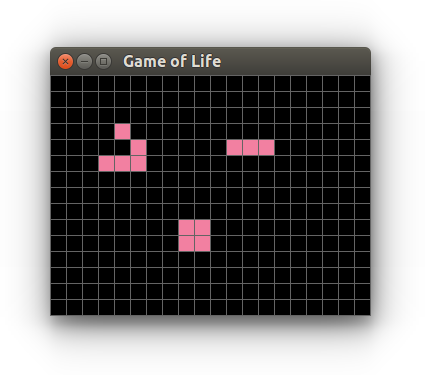
\includegraphics[width=1.0\textwidth]{../img/glider-blinker-block}

  \begin{itemize}\SlideFontTiny
  \item Du ska simulera \emph{Game of Life} i ett \code{introprog.PixelWindow}
  \item Fördjupning:\\{\SlideFontTiny\url{https://en.wikipedia.org/wiki/Conway%27s_Game_of_Life}}
  \end{itemize}
\end{minipage}%

\end{Slide}






\Subsection{Matriser}

\begin{Slide}{Vad är en matris?}\SlideFontSmall
\begin{itemize}

\item En \Emph{matris} inom \Alert{matematiken} innehåller \Emph{rader} och \Emph{kolumner}\footnote{även kallade \emph{kolonner}} med tal.

\item I en \Alert{matematisk} matris har alla rader \Emph{lika många} element och

\item även alla kolumner har \Emph{lika många} element.

\item En matris av dimension $2\times{}5$ har $2 \cdot 5 = 10$ stycken element.

\item Exempel på en matematisk matris av dimension $2\times{}5$:
\[
M_{2,5}=
  \begin{pmatrix}
    5 & 2 & 42 & 4 & 5 \\
    3 & 4 & 18 & 6 & 7
  \end{pmatrix}
\]
\end{itemize}
\end{Slide}

\begin{Slide}{Indexering i en matris}\SlideFontSmall
\begin{itemize}

  \item En matris av dimension $m\times{}n$ har $m \cdot n$ stycken element.

  \item En matris $A_{m,n}$ av dimension $m\times{}n$ ritas inom matematiken ofta så här:

  \[
  A_{m,n} =
   \begin{pmatrix}
    a_{1,1} & a_{1,2} & \cdots & a_{1,n} \\
    a_{2,1} & a_{2,2} & \cdots & a_{2,n} \\
    \vdots  & \vdots  & \ddots & \vdots  \\
    a_{m,1} & a_{m,2} & \cdots & a_{m,n}
   \end{pmatrix}
  \]


\item Matrisindexering inom matematiken sker ofta från $1$, men ofta från $0$ i datorprogram.

\item Vad har talet $42$ för index i matrisen $M_{2,5}$ nedan?
\begin{itemize}\SlideFontTiny
  \item[--] Inom matematiken?
  \item[--] I Scala och Java och många andra språk?

  \[
  M_{2,5}=
    \begin{pmatrix}
      5 & 2 & 42 & 4 & 5 \\
      3 & 4 & 18 & 6 & 7
    \end{pmatrix}
  \]
\end{itemize}
\end{itemize}
\end{Slide}

\begin{Slide}{En matris med array av arrayer}
Inom programmering används ordet \Emph{matris} ofta för att beteckna en \Alert{nästlad struktur} i två dimensioner, till exempel en instans av typen \code{Array[Array[Int]]}
\begin{REPL}
scala> val xss = Array(Array(5,2,42,4,5),Array(3,4,18,6,7))
xss: Array[Array[Int]] = Array(Array(5, 2, 42, 4, 5), Array(3, 4, 18, 6, 7))
\end{REPL}
\pause
Man indexerar i en nästlad sekvens med upprepad \code{apply}:
\begin{REPL}
scala> xss(0)(2)
res0: ???                   // Vad är typ och värde?

scala> xss.apply(0).apply(2)
res1: ???                   // Vad är typ och värde?

scala> xss(0)
res2: ???                   // Vad är typ och värde?
\end{REPL}

\end{Slide}

\begin{Slide}{En matris med array av arrayer}
Inom programmering används ordet \Emph{matris} ofta för att beteckna en \Alert{nästlad struktur} i två dimensioner, till exempel en instans av typen \code{Array[Array[Int]]}
\begin{REPL}
scala> val xss = Array(Array(5,2,42,4,5),Array(3,4,18,6,7))
xss: Array[Array[Int]] = Array(Array(5, 2, 42, 4, 5), Array(3, 4, 18, 6, 7))
\end{REPL}

Man indexerar i en nästlad sekvens med upprepad \code{apply}:
\begin{REPL}
scala> xss(0)(2)
res0: Int = 42

scala> xss.apply(0).apply(2)
res1: Int = 42

scala> xss(0)
res2: Array[Int] = Array(5, 2, 42, 4, 5)
\end{REPL}
\end{Slide}

\begin{Slide}{Uppdatering av en förändringsbar nästlad struktur}
Man kan förändra en array av arrayer ''på plats'' med tilldelning:
\begin{REPL}
scala> val xss = Array(Array(5,2,42,4,5),Array(3,4,18,6,7))

scala> xss(0)(0) = 100

scala> xss
res0: ???

scala> xss(0)(2) = xss(0)(2) - 1

scala> xss
res1: ???

scala> xss(1) = Array.fill(5)(-1)

scala> xss
res2: ???
\end{REPL}
\end{Slide}

\begin{Slide}{Uppdatering av en förändringsbar nästlad struktur}
Man kan förändra en array av arrayer ''på plats'' med tilldelning:
\begin{REPL}
scala> val xss = Array(Array(5,2,42,4,5),Array(3,4,18,6,7))

scala> xss(0)(0) = 100

scala> xss
res0: Array[Array[Int]]=Array(Array(100, 2, 42, 4, 5), Array(3, 4, 18, 6, 7))

scala> xss(0)(2) = xss(0)(2) - 1

scala> xss
res1: Array[Array[Int]]=Array(Array(100, 2, 41, 4, 5), Array(3, 4, 18, 6, 7))

scala> xss(1) = Array.fill(5)(-1)

scala> xss
res2: Array[Array[Int]]=Array(Array(100, 2, 41, 4, 5), Array(-1,-1,-1,-1,-1))
\end{REPL}
\end{Slide}

\begin{Slide}{Några olika sätt att skapa förändringsbara matriser}\SlideFontSmall
Det jobbiga, primitiva sättet:
\begin{REPL}
scala> val xs = new Array[Array[Int]](2)
xs: Array[Array[Int]] = Array(null, null)

scala> for (i <- xs.indices) {xs(i) = new Array[Int](5)}

scala> xs
res0: Array[Array[Int]] = Array(Array(0, 0, 0, 0, 0), Array(0, 0, 0, 0, 0))

scala> println(xs)
[[I@196a99d0
\end{REPL}
Enklare sätt:
\begin{REPL}
scala> val xs = Array.ofDim[Int](2,5)
xs: Array[Array[Int]] = Array(Array(0, 0, 0, 0, 0), Array(0, 0, 0, 0, 0))
\end{REPL}
Enklare och tydligare sätt, där initialvärdet anges explicit:
\begin{REPL}
scala> Array.fill(2,5)(0)
res37: Array[Array[Int]] = Array(Array(0, 0, 0, 0, 0), Array(0, 0, 0, 0, 0))
\end{REPL}

\end{Slide}

\begin{Slide}{Exempel på skapande av oföränderlig nästlad struktur}\SlideFontSmall
Om du kan beräkna initialvärde direkt, använd \code{Vector.fill}:\\
{\SlideFontTiny\code{def fill[A](n1: Int, n2: Int)(elem: => A): Vector[Vector[A]]}}
\begin{REPL}
scala> Vector.fill(2,5)(scala.util.Random.nextInt(6) + 1)
res0:
  typ???
  värde???

\end{REPL}
Om du kan beräkna initialvärde ur index, använd \code{Vector.tabulate}:\\
{\SlideFontTiny\code{def tabulate[A](n1: Int, n2: Int)(f: (Int, Int) => A): Vector[Vector[A]]}}
\begin{REPL}
scala> Vector.tabulate(5,2)((x,y) => x + y + 1)
res1:
  typ???
  värde???

\end{REPL}
\end{Slide}

\begin{Slide}{Exempel på skapande av oföränderlig nästlad struktur}\SlideFontSmall
Om du kan beräkna initialvärde direkt, använd \code{Vector.fill}:\\
{\SlideFontTiny\code{def fill[A](n1: Int, n2: Int)(elem: => A): Vector[Vector[A]]}}
\begin{REPL}
scala> Vector.fill(2,5)(scala.util.Random.nextInt(6) + 1)
res0:
  scala.collection.immutable.Vector[scala.collection.immutable.Vector[Int]] =
  Vector(Vector(1, 2, 6, 2, 1), Vector(1, 4, 3, 3, 2))

\end{REPL}
Om du kan beräkna initialvärde ur index, använd \code{Vector.tabulate}:\\
{\SlideFontTiny\code{def tabulate[A](n1: Int, n2: Int)(f: (Int, Int) => A): Vector[Vector[A]]}}
\begin{REPL}
scala> Vector.tabulate(5,2)((x,y) => x + y + 1)
res1:
  scala.collection.immutable.Vector[scala.collection.immutable.Vector[Int]] =
  Vector(Vector(1,2), Vector(2,3), Vector(3,4), Vector(4,5), Vector(5,	6))

\end{REPL}
\end{Slide}



\begin{Slide}{Uppdatering av en oföränderlig nästlad struktur}\SlideFontSmall
Uppdatering av endimensionell struktur med \code{xs.updated}:\\
{\SlideFontTiny\code{def updated[A](index: Int, elem: A): Vector[A]} }
\begin{REPL}
scala> var xs = Vector.tabulate(5)(x => x + 1)
xs: typ??? = värde???

scala> xs = xs.updated(1, 42)
xs: typ??? = värde???
\end{REPL}

Uppdatering av nästlad struktur i två dimensioner:
\begin{REPL}
scala> var xss = Vector.tabulate(2, 5)((x,y) => x + y + 1)
xss:
  typ??? =
  värde???

scala> xss = xss.updated(0, xss(0).updated(1, 42))
xss:
  typ??? =
  värde???
\end{REPL}

\end{Slide}



\begin{Slide}{Uppdatering av en oföränderlig nästlad struktur}\SlideFontSmall
Uppdatering av endimensionell struktur med \code{xs.updated}:\\
{\SlideFontTiny\code{def updated[A](index: Int, elem: A): Vector[A]} }
\begin{REPL}
scala> var xs = Vector.tabulate(5)(x => x + 1)
xs: scala.collection.immutable.Vector[Int] = Vector(1, 2, 3, 4, 5)

scala> xs = xs.updated(1, 42)
xs: scala.collection.immutable.Vector[Int] = Vector(1, 42, 3, 4, 5)
\end{REPL}

Uppdatering av nästlad struktur i två dimensioner:
\begin{REPL}
scala> var xss = Vector.tabulate(2, 5)((x,y) => x + y + 1)
xss:
  scala.collection.immutable.Vector[scala.collection.immutable.Vector[Int]] =
  Vector(Vector(1, 2, 3, 4, 5), Vector(2, 3, 4, 5, 6))

scala> xss = xss.updated(0, xss(0).updated(1, 42))
xss:
  scala.collection.immutable.Vector[scala.collection.immutable.Vector[Int]] =
  Vector(Vector(1, 42, 3, 4, 5), Vector(2, 3, 4, 5, 6))
\end{REPL}

\end{Slide}


\begin{Slide}{Iterera över nästlad struktur: for-sats}\SlideFontSmall
Iterera med nästlad for-sats:
\begin{REPL}
scala> val xss = Vector.tabulate(2,5)((x,y) => x + y + 1)

scala> for (???) {
         for (???) {
           print(xss(i)(j) + " ")
         }
         println
       }

1 2 3 4 5
2 3 4 5 6
\end{REPL}
\end{Slide}

\begin{Slide}{Iterera över nästlad struktur: for-sats}\SlideFontSmall
Iterera med nästlad for-sats:
\begin{REPL}
scala> val xss = Vector.tabulate(2,5)((x,y) => x + y + 1)

scala> for (i <- xss.indices) {
         for (j <- xss(i).indices) {
           print(xss(i)(j) + " ")
         }
         println
       }

1 2 3 4 5
2 3 4 5 6
\end{REPL}
\end{Slide}


\begin{Slide}{Övningsexempel: Yatzy}\SlideFontSmall
Skapa en funktion \code{roll} som ger utfallet av n st tärningskast:
\begin{REPL}
scala> import scala.util.Random

scala> def roll(n: Int): Vector[Int] = ???
\end{REPL}

Skapa en funktion \code{isYatzy} som ger \code{true} om alla utfall är lika:
\begin{REPL}
scala> def isYatzy(xs: Vector[Int]): Boolean = ???
\end{REPL}
Du kan anta att xs.length > 0\\
Tips: använd metoden xs.forall: \\
\code{def forall[A](p: A => Boolean): Boolean }
\end{Slide}


\begin{Slide}{Övningsexempel: Yatzy}\SlideFontSmall
Skapa en funktion \code{roll} som ger utfallet av n st tärningskast:
\begin{REPL}
scala> import scala.util.Random

scala> def roll(n: Int): Vector[Int] = Vector.fill(n)(Random.nextInt(6) + 1)
\end{REPL}

Skapa en funktion \code{isYatzy} som ger \code{true} om alla utfall är lika:
\begin{REPL}
scala> def isYatzy(xs: Vector[Int]): Boolean = xs.forall(x => x == xs(0))
\end{REPL}
Du kan anta att xs.length > 0\\
Tips: använd metoden xs.forall: \\
\code{def forall[A](p: A => Boolean): Boolean }
\end{Slide}

\begin{Slide}{Iterera över nästlad struktur: for-sats}\SlideFontSmall
Iterera med nästlad for-sats: (vad har xss för typ?)
\begin{REPL}
scala> val xss = Vector.fill(100)(roll(5))

scala> for (???) {
         for (???) {
           print(s"($i)($j) == " + xss(i)(j) + " ")
         }
         println(isYatzy(???))
       }

(0)(0) == 5 (0)(1) == 3 (0)(2) == 4 (0)(3) == 1 (0)(4) == 3 false
(1)(0) == 3 (1)(1) == 3 (1)(2) == 6 (1)(3) == 3 (1)(4) == 1 false
(2)(0) == 3 (2)(1) == 4 (2)(2) == 2 (2)(3) == 2 (2)(4) == 1 false
(3)(0) == 5 (3)(1) == 2 (3)(2) == 6 (3)(3) == 5 (3)(4) == 1 false
(4)(0) == 4 (4)(1) == 6 (4)(2) == 4 (4)(3) == 1 (4)(4) == 4 false
(5)(0) == 3 (5)(1) == 4 (5)(2) == 6 (5)(3) == 5 (5)(4) == 1 false
(6)(0) == 4 (6)(1) == 6 (6)(2) == 2 (6)(3) == 2 (6)(4) == 6 false
(7)(0) == 2 (7)(1) == 5 (7)(2) == 3 (7)(3) == 6 (7)(4) == 2 false
(8)(0) == 4 (8)(1) == 4 (8)(2) == 6 (8)(3) == 1 (8)(4) == 4 false
(9)(0) == 3 (9)(1) == 3 (9)(2) == 3 (9)(3) == 3 (9)(4) == 3 true
(10)(0) == 1 (10)(1) == 2 (10)(2) == 4 (10)(3) == 3 (10)(4) == 3 false
(11)(0) == 6 (11)(1) == 5 (11)(2) == 4 (11)(3) == 1 (11)(4) == 5 false
(12)(0) == 3 (12)(1) == 6 (12)(2) == 6 (12)(3) == 4 (12)(4) == 2 false
\end{REPL}
\end{Slide}

\begin{Slide}{Iterera över nästlad struktur: for-sats}\SlideFontSmall
Iterera med nästlad for-sats: (xss är en \code{Vector[Vector[Int]]})
\begin{REPL}
scala> val xss = Vector.fill(100)(roll(5))

scala> for (i <- xss.indices) {
         for (j <- xss(i).indices) {
           print(s"($i)($j) == " + xss(i)(j) + " ")
         }
         println(isYatzy(xss(i)))
       }

(0)(0) == 5 (0)(1) == 3 (0)(2) == 4 (0)(3) == 1 (0)(4) == 3 false
(1)(0) == 3 (1)(1) == 3 (1)(2) == 6 (1)(3) == 3 (1)(4) == 1 false
(2)(0) == 3 (2)(1) == 4 (2)(2) == 2 (2)(3) == 2 (2)(4) == 1 false
(3)(0) == 5 (3)(1) == 2 (3)(2) == 6 (3)(3) == 5 (3)(4) == 1 false
(4)(0) == 4 (4)(1) == 6 (4)(2) == 4 (4)(3) == 1 (4)(4) == 4 false
(5)(0) == 3 (5)(1) == 4 (5)(2) == 6 (5)(3) == 5 (5)(4) == 1 false
(6)(0) == 4 (6)(1) == 6 (6)(2) == 2 (6)(3) == 2 (6)(4) == 6 false
(7)(0) == 2 (7)(1) == 5 (7)(2) == 3 (7)(3) == 6 (7)(4) == 2 false
(8)(0) == 4 (8)(1) == 4 (8)(2) == 6 (8)(3) == 1 (8)(4) == 4 false
(9)(0) == 3 (9)(1) == 3 (9)(2) == 3 (9)(3) == 3 (9)(4) == 3 true
(10)(0) == 1 (10)(1) == 2 (10)(2) == 4 (10)(3) == 3 (10)(4) == 3 false
(11)(0) == 6 (11)(1) == 5 (11)(2) == 4 (11)(3) == 1 (11)(4) == 5 false
(12)(0) == 3 (12)(1) == 6 (12)(2) == 6 (12)(3) == 4 (12)(4) == 2 false
\end{REPL}
\end{Slide}


\begin{Slide}{Iterera över nästlad struktur med nästlad foreach}\SlideFontSmall
Iterera med nästlad foreach-sats:
\begin{REPL}
scala> val xss = Vector.tabulate(2,5)((x,y) => x + y + 1)

xss.foreach{ xs => ??? ; println }

1 2 3 4 5
2 3 4 5 6
\end{REPL}
\end{Slide}


\begin{Slide}{Iterera över nästlad struktur med nästlad foreach}\SlideFontSmall
Iterera med nästlad foreach-sats:
\begin{REPL}
scala> val xss = Vector.tabulate(2,5)((x,y) => x + y + 1)

xss.foreach{ xs => xs.foreach{ x => print(x + " ") }; println }

1 2 3 4 5
2 3 4 5 6
\end{REPL}
\end{Slide}


\begin{Slide}{Nästlade for-uttryck}\SlideFontSmall
Iterera med \Emph{nästlad for-yield}:\\
%Statisk typ: \code{IndexedSeq[IndexedSeq[[Int]]} \\
%Dynamisk typ: \code{Vector[Vector[[Int]]}

\begin{REPL}
scala> val xss = for (i <- 1 to 2) yield {
                   for (j <- 1 to 5) yield i + j + 1
                 }
xss:
  scala.collection.immutable.IndexedSeq[
    scala.collection.immutable.IndexedSeq[Int]] =
      ???

\end{REPL}
Om man skriver så här får man en endimensionell struktur:
\begin{REPL}
scala> val xs = for (i <- 1 to 2; j <- 1 to 5) yield i + j + 1
xs:
  scala.collection.immutable.IndexedSeq[Int] =
    ???

\end{REPL}
\end{Slide}

\begin{Slide}{Nästlade for-uttryck}\SlideFontSmall
Iterera med \Emph{nästlad for-yield}:\\
\begin{REPL}
scala> val xss = for (i <- 1 to 2) yield {
                   for (j <- 1 to 5) yield i + j + 1
                 }
xss:
  scala.collection.immutable.IndexedSeq[
    scala.collection.immutable.IndexedSeq[Int]] =
      Vector(Vector(3, 4, 5, 6, 7), Vector(4, 5, 6, 7, 8))

\end{REPL}
Om man skriver så här får man en endimensionell struktur:
\begin{REPL}
scala> val xs = for (i <- 1 to 2; j <- 1 to 5) yield i + j + 1
xs:
  scala.collection.immutable.IndexedSeq[Int] =
    Vector(3, 4, 5, 6, 7, 4, 5, 6, 7, 8)

\end{REPL}
\end{Slide}



\begin{Slide}{Nästlade map-uttryck}\SlideFontSmall
Iterera med \Emph{nästlade map-uttryck}:\\
\begin{REPL}
scala> val xss = (1 to 2).map(i => (1 to 5).map(j => i + j + 1))
xss:
  scala.collection.immutable.IndexedSeq[
    scala.collection.immutable.IndexedSeq[Int]] =
      ???
\end{REPL}
\end{Slide}

\begin{Slide}{Nästlade map-uttryck}\SlideFontSmall
Iterera med \Emph{nästlade map-uttryck}:\\
\begin{REPL}
scala> val xss = (1 to 2).map(i => (1 to 5).map(j => i + j + 1))
xss:
  scala.collection.immutable.IndexedSeq[
    scala.collection.immutable.IndexedSeq[Int]] =
      Vector(Vector(3, 4, 5, 6, 7), Vector(4, 5, 6, 7, 8))
\end{REPL}
\end{Slide}




\begin{Slide}{Matris som Array med Array med heltal i Java}\SlideFontTiny
\begin{CodeSmall}[language=Java]
public class ArrayMatrix {

    public static void showMatrix(int[][] m){
        System.out.println("\n--- showMatrix ---");
        for (int row = 0; row < m.length; row++){
            for (int col = 0; col < m[row].length; col++) {
                System.out.print("[" + row + "]");
                System.out.print("[" + col + "] = ");
                System.out.print(m[row][col] + "; ");
            }
            System.out.println();
        }
    }

    public static void main(String[] args) {
        int[][] xss = new int[10][5];
        showMatrix(xss);
    }
}
\end{CodeSmall}
\pause
Övning: skriv en metod \code{fillRnd} som fyller en heltalsmatris med slumptal 1 till n:
\pause
\jcode|public static void fillRnd(int[][] m, int n){ /* ??? */ }| \\
\pause
Tips: använd en nästlad for-sats och: \\
\jcode{(int) (Math.random * n + 1)   // (int) motsvarar Scalas asInstanceOf[Int]}

\end{Slide}

\begin{Slide}{Om veckans övningar}\SlideFontSmall
\begin{itemize}
\item Träna på att iterera i nästlade strukurer

\item Fortsätt jobba med Yatzy-exemplet

\item träna på att skapa \Emph{imperativa} algoritmer: \\
lös \code{isYatzy} med \code{while}-sats (kunde varit del av en tenta...)

\item Extrauppgift där du ska bygga ett enkelt yatzy-spel i terminalen (kunde varit en tentauppgift...)

\end{itemize}
\end{Slide}

% \begin{Slide}{Övning extrauppgift, utgör början på labb \code{survey}}\SlideFontSmall
%
% \begin{ScalaSpec}{Table}
% object Table {
%   /** Creates a new Table from fileName with columns split by sep */
%   def fromFile(fileName: String, separator: Char = ';'): Table = ???
% }
% case class Table(
%   data: Vector[Vector[String]],
%   headings: Vector[String],
%   sep: String){
%   /** A 2-tuple with (number of rows, number of columns) in data */
%   val dim: (Int, Int) = ???
%
%   /** The element in row r an column c of data, counting from 0 */
%   def apply(r: Int, c: Int): String = ???
%
%   /** The row-vector r in data, counting from 0 */
%   def row(r: Int): Vector[String]= ???
%
%   /** The column-vector c in data, counting from 0 */
%   def col(c: Int): Vector[String] = ???
%
%   /** A map from heading to index counting from 0 */
%   lazy val indexOfHeading: Map[String, Int] = ???
%
%   /** The column-vector with heading h in data */
%   def col(h: String): Vector[String] = ???
%
%   /** A vector with the distinct, sorted values of col with heading h */
%   def values(h: String): Vector[String] = ???
%
%   /** Headings and data with columns separated by sep */
%   override lazy val toString: String = ???
% }
% \end{ScalaSpec}
% \end{Slide}


% \begin{Slide}{Övn. fördjupn. uppg.: skapa en generisk matris-klass}\SlideFontSmall
% \vspace{-0.7em}
% \begin{Code}[basicstyle=\SlideFontSize{6}{6.8}\ttfamily\selectfont]
% case class Matrix[T](data: Vector[Vector[T]]){
%
%   def foreachRowCol(f: (Int, Int, T) => Unit): Unit =
%     for (r <- data.indices) {
%       for (c <- data(r).indices) {
%         f(r, c, data(r)(c))
%       }
%     }
%
%   def map[U](f: T => U): Matrix[U] = Matrix(data.map(_.map(f)))
%
%   /** The element at row r and column c */
%   def apply(r: Int, c: Int): T = ???
%
%   /** Gives Some[T](element) at index (r, c) if within index bounds, else None */
%   def get(r: Int, c: Int): Option[T] = ???
%
%   /** The row vector of row r */
%   def row(r: Int): Vector[T] = ???
%
%   /** The column vector of column c */
%   def col(c: Int): Vector[T] = ???
%
%   /** A new Matrix with element at row r and col c updated */
%   def updated(r: Int, c: Int, value: T): Matrix[T] = ???
% }
% object Matrix {
%   def fill[T](rowSize: Int, colSize: Int)(init: T): Matrix[T] =
%     new Matrix(Vector.fill(rowSize)(Vector.fill(colSize)(init)))
% }
% \end{Code}
% \end{Slide}

%!TEX encoding = UTF-8 Unicode
%!TEX root = ../lect-w08.tex

\Subsection{Typparametrar}



\begin{Slide}{Exempel: Icke-generisk case-klass med heltalsmatris}
  En \emph{icke-generisk} datastruktur har inga obundna typparametrar; alla typer är \Emph{konkreta} (alltså specifika). \\~\\ En icke-generisk case-class med en \code{Vector[Vector[Int]]}:
  \begin{Code}
  case class Matrix(data: Vector[Vector[Int]]){
    def apply(x: Int, y: Int): Int = data(x)(y)
  }
  \end{Code}

  \begin{REPL}
  scala> Matrix(Vector(Vector(5, 2, 42, 4, 5),Vector(3, 4, 18, 6, 7)))
  res0: Matrix =
    Matrix(Vector(Vector(5, 2, 42, 4, 5), Vector(3, 4, 18, 6, 7)))
  \end{REPL}

\end{Slide}





\begin{Slide}{Exempel: Generisk case-klass med generell matris}
  En \emph{generisk} datastruktur har en \Emph{typparameter} som är \Alert{abstrakt} (alltså generell) som kan bindas  till ett \Alert{konkret} \Emph{typargument}. \\~\\
  En generisk case-class med en \code{Vector[Vector[T]]}:
  \begin{Code}
  case class Matrix[T](data: Vector[Vector[T]]){
    def apply(x: Int, y: Int): T = data(x)(y)
  }
  \end{Code}

  \begin{REPL}
  scala> Matrix(Vector(Vector(5, 2, 42, 4, 5),Vector(3, 4, 18, 6, 7)))
  res1: Matrix[Int] =
    Matrix(Vector(Vector(5, 2, 42, 4, 5), Vector(3, 4, 18, 6, 7)))
  \end{REPL}

\end{Slide}




\begin{Slide}{Vad är en typparameter?}\SlideFontSmall
  \setlength{\leftmargini}{0pt}

\begin{itemize}
\item En \Emph{typparameter} gör det möjligt att ge ett \Emph{typargument}
\item En \Emph{fri} typparameter kan bindas till vilken typ som helst
\item Bindingen sker vid \Alert{kompileringstid}
\item En typparameter är \Emph{fri} om den \Alert{inte} fått något värde i omslutande deklarationer, annars \Emph{bunden}.
\end{itemize}
Exempel: \Emph{generisk} funktion:
\begin{Code}
def tnirp[A](x: A):Unit = println(x.toString.reverse) // A fri
\end{Code}
\pause
Exempel: \Emph{generisk} klass med generiska metoder:
\begin{Code}
class Cell[A](var value: A){                          // A fri
  def update(x: A): Unit = value = x                  // A bunden
  def create[B](x: B = value): Cell[B] = new Cell(x)  // B fri
}
\end{Code}
\pause
\begin{itemize}
\item \Alert{Skuggning kan förekomma}: Om \code{create} i \code{Cell} hade använt namnet A på sin typparameter hade den \Emph{skuggat} klassens typparameter och tolkats som en  fri typparameter och metoden hade fungerat på samma sätt. (jämför med namnöverskuggning vid lokala variabler i nästlade block)
\end{itemize}

\end{Slide}

\ifkompendium\else
\begin{Slide}{Exempel: Generisk funktion}
Vad händer här?
\begin{REPL}

scala> def skrikBaklänges(x: T): String = x.toString.toUpperCase.reverse
???



scala> def skrikBaklänges[T](x: T): String = x.toString.toUpperCase.reverse

scala> skrikBaklänges("gurka är gott")
res0: ???

\end{REPL}
\end{Slide}


\begin{Slide}{Exempel: Generisk funktion}
Vad händer här?
\begin{REPL}

scala> def skrikBaklänges(x: T): String = x.toString.toUpperCase.reverse
<console>:11: error: not found: type T
       def skrikBaklänges(x: T): String = x.toString.toUpperCase.reverse
                             ^

scala> def skrikBaklänges[T](x: T): String = x.toString.toUpperCase.reverse

scala> skrikBaklänges("gurka är gott")
res0: ???
\end{REPL}
\end{Slide}
\fi

\begin{Slide}{Exempel: Generisk funktion}
Vad händer här?
\begin{REPL}

scala> def skrikBaklänges(x: T): String = x.toString.toUpperCase.reverse
<console>:11: error: not found: type T
       def skrikBaklänges(x: T): String = x.toString.toUpperCase.reverse
                             ^

scala> def skrikBaklänges[T](x: T): String = x.toString.toUpperCase.reverse

scala> skrikBaklänges("gurka är gott")
res0: String = TTOG RÄ AKRUG
\end{REPL}
\end{Slide}

\ifkompendium\else
\begin{Slide}{Exempel: Generisk case-klass}
\vspace{-0.5em}\begin{REPL}
scala> def skrikBaklänges[T](x: T): String = x.toString.toUpperCase.reverse

scala> case class Grönsak(whatever: A)
???


scala> case class Grönsak[A](whatever: A)

scala> Grönsak("gurka")
res1: ???

scala> skrikBaklänges(Grönsak(42))
res2: ???

scala> Grönsak[Int](42)
res3: ???

scala> Grönsak[String](42)
???



                       ^
\end{REPL}
\end{Slide}
\fi

\begin{Slide}{Exempel: Generisk case-klass}
\vspace{-0.5em}\begin{REPL}
scala> def skrikBaklänges[T](x: T): String = x.toString.toUpperCase.reverse

scala> case class Grönsak(whatever: A)
<console>:11: error: not found: type A
       case class Grönsak(whatever: A)
                                    ^
scala> case class Grönsak[A](whatever: A)

scala> Grönsak("gurka")
res1: Grönsak[String] = Grönsak(gurka)

scala> skrikBaklänges(Grönsak(42))
res2: String = )24(KASNÖRG

scala> Grönsak[Int](42)
res3: Grönsak[Int] = Grönsak(42)

scala> Grönsak[String](42)
<console>:14: error: type mismatch;
 found   : Int(42)
 required: String
       Grönsak[String](42)
                       ^
\end{REPL}
\end{Slide}


\ifkompendium\else
\begin{Slide}{Fallgrop: likhet av array}
\begin{REPL}
scala> Vector.fill(5)(42) == Vector.fill(5)(42)
res0: ???

scala> Array.fill(5)(42) == Array.fill(5)(42)
res1: ???
\end{REPL}
\end{Slide}
\fi

\begin{Slide}{Fallgrop: likhet av array}
\begin{REPL}
scala> Vector.fill(5)(42) == Vector.fill(5)(42)
res0: Boolean = true

scala> Array.fill(5)(42) == Array.fill(5)(42)
res1: Boolean = false  // AAAARRGH!!! :(
\end{REPL}
Primitiva arrayer har en equals-metod som ger referenslikhet, \Alert{inte} innehållslikhet.
\end{Slide}

\ifkompendium\else
\begin{Slide}{Kolla likhet av array-matris med nästlad while}
\begin{REPL}
scala> def isEqual(xss: Array[Array[Int]], yss: Array[Array[Int]]) = {
         var i = 0
         var foundUnequal = false
         while (???) {
           var j = 0
           while (???) {
             if (xss(i)(j) != yss(i)(j)) ???
             j += 1
           }
           i += 1
         }
         !foundUnequal
       }

scala> val (xss, yss) = (Array.fill(5,2)(42), Array.fill(5,2)(42))

scala> isEqual(xss, yss)

scala> yss(4)(1) = 0

scala> isEqual(xss, yss)
\end{REPL}
\end{Slide}
\fi


\begin{Slide}{Kolla likhet av array-matris med nästlad while}
\begin{REPL}
scala> def isEqual(xss: Array[Array[Int]], yss: Array[Array[Int]]) = {
         var i = 0
         var foundUnequal = false
         while (i < xss.length && !foundUnequal) {
           var j = 0
           while (j < xss(i).length && !foundUnequal) {
             if (xss(i)(j) != yss(i)(j)) foundUnequal = true
             j += 1
           }
           i += 1
         }
         !foundUnequal
       }

scala> val (xss, yss) = (Array.fill(5,2)(42), Array.fill(5,2)(42))

scala> isEqual(xss, yss)

scala> yss(4)(1) = 0

scala> isEqual(xss, yss)
\end{REPL}
\end{Slide}


\ifkompendium\else
\begin{Slide}{Fördjupning: Fallgrop typradering \Eng{type erasure}}\SlideFontSmall
Informationen om typerna i typparametrar raderas innan kodgenerering av prestandaskäl och \Alert{typparametrar saknas vid runtime}.
\vspace{-0.25em}\begin{REPL}
scala> val xs = Vector(1,2,3)
xs: scala.collection.immutable.Vector[Int] = Vector(1, 2, 3)

scala> val ys = xs.map(_.toDouble)
ys: scala.collection.immutable.Vector[Double] = Vector(1.0, 2.0, 3.0)

scala> def hasDoubles[T](xs: Vector[T]): Boolean = xs match {
         case _: Vector[Int] => false
         case _: Vector[Double] => true
       }

<console>:13: warning: ???


                        ^
<console>:14: warning: ???


                        ^
<console>:14: warning: ???
\end{REPL}
\end{Slide}
\fi

\begin{Slide}{Fördjupning: Fallgrop typradering \Eng{type erasure}}\SlideFontSmall
Informationen om typerna i typparametrar raderas innan kodgenerering av prestandaskäl och \Alert{typparametrar saknas vid runtime}.
\vspace{-0.25em}\begin{REPL}
scala> val xs = Vector(1,2,3)
xs: scala.collection.immutable.Vector[Int] = Vector(1, 2, 3)

scala> val ys = xs.map(_.toDouble)
ys: scala.collection.immutable.Vector[Double] = Vector(1.0, 2.0, 3.0)

scala> def hasDoubles[T](xs: Vector[T]): Boolean = xs match {
         case _: Vector[Int] => false
         case _: Vector[Double] => true
       }

<console>:13: warning: non-variable type argument Int in type pattern scala.collection.immutable.Vector[Int]
is unchecked since it is eliminated by erasure
                case _: Vector[Int] => false
                        ^
<console>:14: warning: non-variable type argument Double in type pattern scala.collection.immutable.Vector[Int]
is unchecked since it is eliminated by erasure
                case _: Vector[Double] => true
                        ^
<console>:14: warning: unreachable code: case _: Vector[Double] => true
\end{REPL}
\end{Slide}

\begin{Slide}{Fördjupning: Dynamisk typtest vid typradering}\SlideFontSmall
Typtest vid körtid med nästlad matchning:
\begin{REPL}
scala> def hasDoubles2[T](xs: Vector[T]): Boolean = xs match {
         case x +: xs => x match {
           case _: Double => true
           case _ => false
         }
         case _ => false
       }

scala> hasDoubles2(Vector(1.0))    // funkar!
\end{REPL}

Typtest vid körtid med match och gard med \code{isInstanceOf}:
\begin{REPL}

scala> def hasDoubles3[T](xs: Vector[T]): Boolean = xs match {
         case x +: xs if x.isInstanceOf[Double] => true
         case _ => false
       }

scala> hasDoubles3(Vector(1.0))    // funkar!


\end{REPL}
\end{Slide}


\ifkompendium\else

\begin{Slide}{Typparametrar på tentan?}
\begin{itemize}
\item Det ingår att kunna använda färdiga generiska strukturer med specifika typer, t.ex. \code{Vector[Int]}

\item Det ingår att kunna skapa strukturer med specifika typparametrar, t.ex. en case-klass som tar en vektor med en specifik typ:\\
\code{case class X(x: Vector[Int])}



\item Det ingår \Alert{inte} på tentan att kunna skapa generiska metoder eller klasser, t.ex.: \\
\code{def f[T](x: Vector[T]): Vector[T] = ???} \\
Mer om generiska strukturer i fördjupningskursen!
\end{itemize}
\end{Slide}

\fi

%!TEX encoding = UTF-8 Unicode
%!TEX root = ../lect-w08.tex

% \Subsection{TODO TABORT Integrerad utvecklingsmiljö (IDE)}

% \begin{Slide}{\TODO TABORT Välja IDE}\SlideFontSmall
% \begin{itemize}
% \item En \Emph{integrerad utvecklingsmiljö} \Eng{Integrated Development Environment, IDE} innehåller \\ editor + kompilator + debugger + en massa annat\\och gör utvecklingen enklare när man lärt sig alla finesser.

% \item Läs om vad en IDE kan göra i appendix.

% \pause

% \item På LTH:s datorer finns tre populära IDE installerade:
% \begin{enumerate}\SlideFontSmall

% \item \Emph{VS Code} med tillägget Metals. \Alert{Rekommenderas!}
% \begin{REPL}[numbers=none]
% > code
% \end{REPL}


% \item \Emph{IntelliJ IDEA} med Scala-plugin. Välj denna om du vill ha en IDE som är mer avancerad och är sugen på att lära dig något nytt.
% \begin{REPL}[numbers=none]
% > idea
% \end{REPL}

% \item \Emph{Eclipse} med plugin \Emph{ScalaIDE} förinstallerad, men rekommenderas ej då den ligger efter i Scala-version.
% \begin{REPL}[numbers=none]
% > scalaide
% \end{REPL}

% \end{enumerate}
% %Läs mer om dessa i appendix.
% %  innan du väljer vilken du vill lära dig.
% % \\Där står även hur du installerar dem på din egen dator.
% % \\IntelliJ anses av många för tillfället ha det bästa Scala-stödet, men är du van vid Eclipse så kanske du vill använda ScalaIDE.
% \end{itemize}
% \end{Slide}

% \begin{Slide}{\TODO SKA HANDLA OM DEBUG i VS Code med Scala-plugin Metals}
% 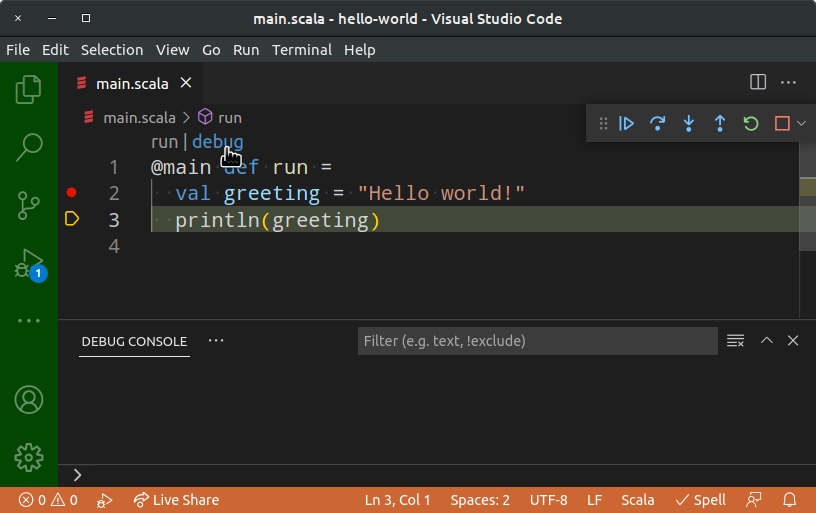
\includegraphics[width=\textwidth]{../img/vscode-debug.png}
% \end{Slide}
  

% \begin{Slide}{IntelliJ IDEA med Scala-plugin}
% 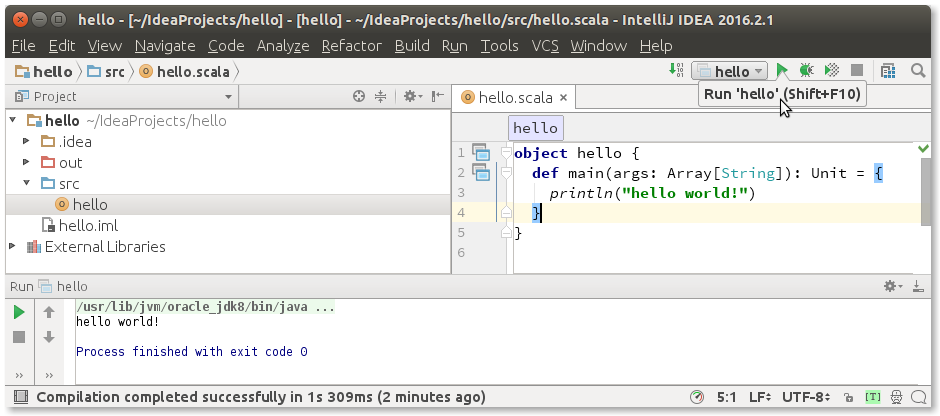
\includegraphics[width=\textwidth]{../img/intellij/idea-hello.png}
% \end{Slide}

% \begin{Slide}{Eclipse med ScalaIDE}
% 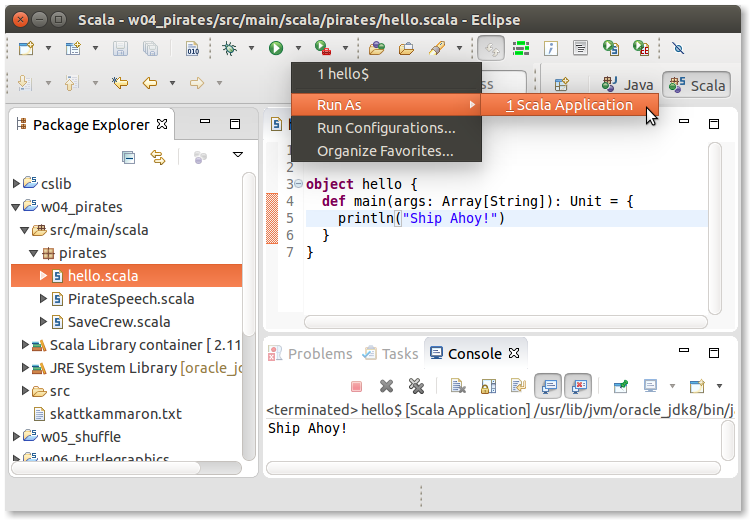
\includegraphics[width=\textwidth]{../img/eclipse/eclipse-pirates-hello.png}
% \end{Slide}




%!TEX encoding = UTF-8 Unicode
%!TEX root = ../exercises.tex

\ifPreSolution

\Exercise{\ExeWeekEIGHT}\label{exe:W08}

\begin{Goals}
\item Kunna skapa och använda matriser med nästlade strukturer av \code{Vector}.
\item Kunna iterera över elementen i en matris med nästlade \code{for}-satser och \code{for}-\code{yield}-uttryck, samt nästlad applicering av \code{map} respektive \code{foreach}.
\item Kunna skapa och använda funktioner som tar matriser som parametrar.
\item Kunna skapa en enkel generisk klass och enkla generiska funktioner med hjälp av en typparameter.
\item Kunna beskriva skillnader och likheter mellan Scala och Java vad gäller indexering och iterering i matriser implementerade med nästlade arrayer.
%\item Kunna skapa och använda matriser med hjälp inbyggda arrayer i Java.
%\item Kunna använda nästlade \code{for}-satser i Java för att iterera över elementen i en matris.
\end{Goals}

\begin{Preparations}
\item \StudyTheory{08}
\end{Preparations}

\BasicTasks

\else

\ExerciseSolution{\ExeWeekEIGHT}

\BasicTasks

\fi



\WHAT{Para ihop begrepp med beskrivning.}

\QUESTBEGIN

\Task \what

\vspace{1em}\noindent Koppla varje begrepp med den (förenklade) beskrivning som passar bäst:

\begin{ConceptConnections}
  matris & 1 & & A & konkret typ, binds till typparameter vid kompilering \\ 
  generisk & 2 & & B & indexerbar datastruktur i två dimensioner \\ 
  typargument & 3 & & C & har abstrakt typparameter, typen är generell \\ 
  typhärledning & 4 & & D & kompilatorn beräknar typ ur sammanhanget \\ 
\end{ConceptConnections}

\SOLUTION

\TaskSolved \what

\begin{ConceptConnections}
  matris & 1 & ~~\Large$\leadsto$~~ &  A & indexerbar datastruktur i två dimensioner \\ 
  radvektor & 2 & ~~\Large$\leadsto$~~ &  F & matris av dimension $1\times{}m$ med $m$ horisontella värden \\ 
  kolumnvektor & 3 & ~~\Large$\leadsto$~~ &  G & matris av dimension $m\times{}1$ med $m$ vertikala värden \\ 
  kolonn & 4 & ~~\Large$\leadsto$~~ &  C & annat ord för kolumn \\ 
  generisk & 5 & ~~\Large$\leadsto$~~ &  B & har abstrakt typparameter, typen är generell \\ 
  typargument & 6 & ~~\Large$\leadsto$~~ &  D & konkret typ, binds till typparameter vid kompilering \\ 
  typhärledning & 7 & ~~\Large$\leadsto$~~ &  E & kompilatorn beräknar typ ur sammanhanget \\ 
\end{ConceptConnections}

\QUESTEND




\WHAT{Skapa matriser med hjälp av nästlade samlingar.}

\QUESTBEGIN

\Task  \what~  Man kan i ett datorprogram, med hjälp av samlingar som innehåller samlingar, skapa nästlade strukturer som kan indexeras i två dimensioner och på så sätt representera en  \textbf{matris}.\footnote{\href{https://sv.wikipedia.org/wiki/Matris}{sv.wikipedia.org/wiki/Matris}}

\Subtask Rita minnessituationen efter tilldelningen på rad 1 nedan. Vad har \code{m} för typ och värde? Vad har \code{m} för dimensioner? Hur sker indexeringen i ett datorprogram jämfört med i matematiken?

\begin{REPL}
scala> val m = Vector((1 to 5).toVector, (3 to 7).toVector)
scala> m.apply(0).apply(1)
scala> m(1)
scala> m(1)(4)
\end{REPL}

\Subtask Vad ger uttrycken på raderna 2, 3 och 4 ovan för värden och typ?

\Subtask Man kan i ett datorprogram mycket väl skapa tvådimensionella, nästlade strukturer där raderna \emph{inte} innehåller samma antal element. Det blir då ingen äkta matris i strikt matematisk mening, men man kallar ofta ändå en sådan struktur för en ''matris''. Vilken typ har variablerna \code{m2}, \code{m3}, \code{m4} och \code{m5} nedan?

\begin{REPL}
scala> val m2 = Vector(Vector(1,2,3),Vector(4,5),Vector(42))
scala> val m3 = Vector(Vector(1,2), Vector(1.0, 2.0, 3.0))
scala> val m4 = m3(1) +: Vector("a") +: m3
scala> val m5 = Vector.fill(42){ m2(1).map(e => (e * math.random()).toInt) }
\end{REPL}

\Subtask Vilken av variablerna \code{m2}, \code{m3}, \code{m4} och \code{m5} ovan representerar en äkta matris i matematisk mening? Vilken är dess dimensioner?

\SOLUTION

\TaskSolved \what

\SubtaskSolved   
\includegraphics{../img/w09-solutions/1a} \\
Typ: \code{Vector[Vector[Int]]}\\
Värde: \code{Vector(Vector(1, 2, 3, 4, 5), Vector(3, 4, 5, 6, 7))} \\
Dimensioner: $2 \times 5$\\
Inom matematiken sker indexering enligt konvention med 1 som lägsta index. I scala är lägsta index 0, man använder s.k. 0-indexering. \footnote{Detta är inte fallet i alla programmeringsspråk, vilket du kan läsa mer om på \url{https://en.wikipedia.org/wiki/Array\_data\_type\#Index\_origin}}

\SubtaskSolved
\begin{REPL}
scala> val m = Vector((1 to 5).toVector, (3 to 7).toVector)
m: Vector[Vector[Int]] = Vector(Vector(1, 2, 3, 4, 5), Vector(3, 4, 5, 6, 7))

scala> m.apply(0).apply(1)
res4: Int = 2

scala> m(1)
res5: Vector[Int] = Vector(3, 4, 5, 6, 7)

scala> m(1)(4)
res6: Int = 7
\end{REPL}

\SubtaskSolved  \\
m2: \code{Vector[Vector[Int]]}\\
m3: \code{Vector[Vector[AnyVal]]}\\
m4: \code{Vector[Vector[Any]]}\\
m5: \code{Vector[Vector[Int]]}

\SubtaskSolved  m5, $42 \times 2$

\QUESTEND





\WHAT{Skapa och iterera över matriser.}

\QUESTBEGIN

\Task  \label{matrices:task:yatzy} \what~  Du ska skapa matriser där varje rad representerar 5 kast med en tärning i spelet Yatzy.\footnote{\href{https://sv.wikipedia.org/wiki/Yatzy}{sv.wikipedia.org/wiki/Yatzy}}


\Subtask Definiera i REPL en funktion \code{def throwDie: Int = ???} som returnerar ett slumptal mellan 1 och 6.

\Subtask Skapa nedan heltalsmatris i REPL. Vilken dimension får matrisen?
\begin{REPL}
scala> val ds1 = for (i <- 1 to 1000) yield 
            for (j <- 1 to 5) yield throwDie
          
\end{REPL}

\Subtask Man kan också använda nedan varianter för att skapa en heltalsmatris. Vilken av varianterna \code{ds1} ... \code{ds6} tycker du är lättast att läsa och förstå? Prova respektive variant i REPL och ange vilken typ på \code{ds1} ... \code{ds6} som härleds av kompilatorn.
\begin{REPL}
val ds2 = (1 to 1000).map(i => (1 to 5).map(j => throwDie))
val ds3 = (1 to 1000).map(i => Vector.fill(5)(throwDie))
val ds4 = for (i <- 1 to 1000) yield Vector.fill(5)(throwDie)
val ds5 = Vector.fill(1000)(Vector.fill(5)(throwDie))
val ds6 = Vector.fill(1000, 5)(throwDie)
\end{REPL}


\Subtask Definiera en funktion \\ \code{def roll(n: Int): Vector[Int] = ???}\\ som ger en heltalsvektor med $n$ stycken slumpvisa tärningskast. Kasten ska vara sorterade i växande ordning; använd för detta ändamål samlingsmetoden \code{sorted}.


\Subtask \label{matrices:subtask:isyatzyforall} Definera i REPL en funktion \code{isYatzy(xs: Vector[Int]): Boolean = ???} som testar om alla elementen i en heltalsvektor är samma. Använd samlingsmetoden \code{forall}.


\Subtask Skapa en funktion  \\ \code{def diceMatrix(m: Int, n: Int): Vector[Vector[Int]] = ???} \\ som med hjälp av funktionen \code{roll} skapar en matris med \code{m} st vektorer med vardera \code{n} slumpvisa tärningskast.


\Subtask \label{matrices:subtask:diceMatrixToString} Skapa en funktion som returnerar en utskriftsvänlig sträng \\ \code{def diceMatrixToString(xss: Vector[Vector[Int]]): String = ???} \\med hjälp av \code{map} och \code{mkString}, som fungerar enligt nedan.
\begin{REPL}
scala> val dm2s = diceMatrixToString(diceMatrix(4, 5))
dm2s: String =
2 2 3 3 4
1 2 2 2 5
1 5 5 5 6
1 2 4 5 5
\end{REPL}



\Subtask Implementera funktionen \\ \code{def filterYatzy(xss: Vector[Vector[Int]]): Vector[Vector[Int]]} \\ som filtrerar fram alla yatzy-rader i matrisen \code{xss} enligt nedan. Använd din funktion \code{isYatzy} och samlingsmetoden \code{filter}.
\begin{REPL}
scala> diceMatrixToString(filterYatzy(diceMatrix(10000, 5)))
res18: String =
3 3 3 3 3
2 2 2 2 2
2 2 2 2 2
6 6 6 6 6
3 3 3 3 3
1 1 1 1 1
6 6 6 6 6
\end{REPL}



\Subtask Implementera funktionen \\
\code{def yatzyPips(xss: Vector[Vector[Int]]): Vector[Int] = ???}\\
som ska ge en vektor med de tärningsvärden som gav yatzy, för kasten i matrisen \code{xss} enligt nedan. Använd din funktion \code{filterYatzy}.
\begin{REPL}
scala> val dm = Vector(Vector(1,2,3,4,5),Vector(4,4,4,4,4),Vector(3,3,3,3,3))
scala> yatzyPips(dm)
val res42: Vector[Int] = Vector(4, 3)
\end{REPL}

\SOLUTION

\TaskSolved \what

\SubtaskSolved
\begin{Code}
def throwDie: Int = (math.random() * 6).toInt + 1
\end{Code}
Eller:
\begin{Code}
def throwDie: Int = scala.util.Random.nextInt(6) + 1
\end{Code}

\SubtaskSolved  Matrisdimension i matematisk notation: $1000 \times 5$, vilket motsvarar en matris med 1000 rader och 5 kolumner.

\SubtaskSolved
\begin{Code}
ds1: IndexedSeq[IndexedSeq[Int]]
ds2: IndexedSeq[IndexedSeq[Int]]
ds3: IndexedSeq[Vector[Int]]
ds4: IndexedSeq[Vector[Int]]
ds5: Vector[Vector[Int]]
ds6: Vector[Vector[Int]]
\end{Code}
\code{IndexedSeq} och \code{Vector} ovan finns i paketet \code{scala.collection.immutable}

\SubtaskSolved  \begin{Code}
def roll(n: Int) = Vector.fill(n)(throwDie).sorted
\end{Code}

\SubtaskSolved  \begin{Code}
def isYatzy(xs: Vector[Int]): Boolean = xs.forall(_ == xs(0))
\end{Code}



%2.g)
\SubtaskSolved  \begin{Code}
def diceMatrix(m: Int, n: Int): Vector[Vector[Int]] =
  Vector.fill(m)(roll(n))
\end{Code}

\SubtaskSolved  \begin{Code}
def diceMatrixToString(xss: Vector[Vector[Int]]): String =
  xss.map(_.mkString(" ")).mkString("\n")
\end{Code}


%2.j)
\SubtaskSolved
\begin{Code}
def filterYatzy(xss: Vector[Vector[Int]]): Vector[Vector[Int]] =
  xss.filter(isYatzy)
\end{Code}



%2.m)
\SubtaskSolved  \begin{Code}
def yatzyPips(xss: Vector[Vector[Int]]): Vector[Int] =
  filterYatzy(xss).map(_.head)
\end{Code}

\QUESTEND








\WHAT{En oföränderlig, generisk matris-klass till veckans laboration \hyperref[section:lab:\LabWeekEIGHT]{\texttt{\LabWeekEIGHT}}.}

\QUESTBEGIN

\Task\label{exe:matrices:labprep}  \what~Under veckans laboration ska du simulera en enkel form av ''liv'' som består av celler i ett rutnät. För detta ändamål har vi nytta av en matris-klass som du ska implementera steg för steg i denna övning.
Skapa case-klassen nedan med en editor i filen \code{Matrix.scala}. Testa din lösning med hjälp av valfri \hyperref[appendix:ide]{IDE}, t.ex. \code{scalaide} eller \code{idea}.
\begin{Code}
case class Matrix(data: Vector[Vector[String]]){
  def apply(row: Int, col: Int): String = data(row)(col)
}
object Matrix {
  def fill(dim: (Int, Int))(value: String): Matrix =
    Matrix(Vector.fill(dim._1, dim._2)(value))
}
\end{Code}

\begin{REPLnonum}
scala> val m = Matrix.fill(3,4)("hej")
scala> val e = m(2, 2)
\end{REPLnonum}

\Subtask Vad får \code{m} ovan för typ?

\Subtask Vad får \code{e} ovan för typ?

\Subtask På hur många ställen måste du ändra i \code{Matrix} ovan för att den i stället ska representera en matris av heltal?

\Subtask Du ska nu med hjälp av en \textbf{typparameter} göra \code{Matrix} \textbf{generisk} \Eng{generic}, så att den blir en mer användbar matrisklass som kan innehålla element av vilken typ som helst. Genomför följande ändringar i \code{Matrix.scala}:

\begin{itemize}[noitemsep, nolistsep]
  \item Lägg till en typparameter \code{T} inom klammerparenteser efter namnet \code{Matrix} på alla ställen där det förekommer \emph{utom} efter namnet på kompanjonsobjektet\footnote{Singelobjekt kan inte ha typparametrar, men deras medlemmar kan.}.
  \item Byt ut \code{String} mot \code{T} på alla ställen där \code{String} förekommer.
  \item Lägg till en typparameter \code{T} inom klammerparenteser efter \code{def fill}.
\end{itemize}
Testa din generiska klass i REPL genom att skapa en boolesk matris:
\begin{REPLnonum}
scala> val bm = Matrix.fill(3,4)(false)
scala> val be = bm(0, 0)
\end{REPLnonum}

\Subtask Vad får \code{bm} ovan för typ?

\Subtask Vad får \code{be} ovan för typ?

\Subtask Lägg en kodrad i början av klasskroppen som med hjälp av \code{require} garanterar att alla rader i matrisen är lika långa.

\Subtask Lägg till en medlem \code{val dim: (Int, Int)} i klasskroppen efter \code{require}-satsen som ger ett par (alltså en 2-tupel) med antalet rader resp. kolumner i matrisen.

\Subtask Lägg till en metod \code{def updated(row: Int, col: Int)(value: T): Matrix[T]} som ger en ny matris där element på platsen \code{(row, col)} har uppdaterats till \code{value}.

\Subtask Lägg till en metod \code{def foreachIndex(f: (Int, Int) => Unit): Unit} som för varje index i \code{data} applicerar funktionen \code{f}.

\Subtask Lägg till en metod \code{override def toString} som så att en instans av \code{Matrix} visas enligt följande:
\begin{REPLnonum}
scala> val dm = Matrix.fill(3,4)(42.0)
val dm: Matrix[Double] =
Matrix of dim (3,4):
42.0 42.0 42.0 42.0
42.0 42.0 42.0 42.0
42.0 42.0 42.0 42.0
\end{REPLnonum}


\SOLUTION


\TaskSolved \what

\SubtaskSolved Typen på \code{m} blir \code{Matrix}.

\SubtaskSolved Typen på \code{e} blir \code{String}.

\SubtaskSolved Man behöver ändra på 3 ställen från \code{String} till \code{Int}.

\SubtaskSolved Generisk matris \code{Matrix[T]} för element av godtycklig typ \code{T}:

\begin{CodeSmall}
case class Matrix[T](data: Vector[Vector[T]]):
  def apply(row: Int, col: Int): T = data(row)(col)

object Matrix:
  def fill[T](dim: (Int, Int))(value: T): Matrix[T] =
    Matrix[T](Vector.fill(dim._1, dim._2)(value))
\end{CodeSmall}

\SubtaskSolved Tack vare kompilatorns typinferens så får \code{bm} typen \code{Matrix[Boolean]}.

\SubtaskSolved Typen på \code{be} blir \code{Boolean}.

\noindent \SubtaskSolved \SubtaskSolved \SubtaskSolved \SubtaskSolved \SubtaskSolved är alla implementerade i koden nedan: \vspace{-0.5em}
\begin{CodeSmall}
case class Matrix[T](data: Vector[Vector[T]]):
  require(data.forall(row => row.length == data(0).length))

  val dim: (Int, Int) = (data.length, data(0).length)

  def apply(row: Int, col: Int): T = data(row)(col)

  def updated(row: Int, col: Int)(value: T): Matrix[T] =
    Matrix(data.updated(row, data(row).updated(col, value)))

  def foreachIndex(f: (Int, Int) => Unit): Unit =
    for r <- data.indices; c <- data(r).indices do f(r, c)

  override def toString =
    s"""Matrix of dim $dim:\n${ data.map(_.mkString(" ")).mkString("\n") }"""

object Matrix:
  def fill[T](dim: (Int, Int))(value: T): Matrix[T] =
    Matrix[T](Vector.fill(dim._1, dim._2)(value))

\end{CodeSmall}

\QUESTEND


\clearpage

\ExtraTasks %%%%%%%%%%%%%%%%%%%%%%%%%%%%%%%%%%%%%%%%%%%%%%%%%


\WHAT{Imperativa matrisalgoritmer.}

\QUESTBEGIN

\Task  \what~Imperativa angreppssätt är nödvändiga att kunna när du stöter på samlingar och/eller språk som saknar funktionella metoder och/eller funktionsprogrammeringsmöjligheter. Genom att studera imperativa lösningar till de ofta mer koncisa funktionella lösningarna, får du träning i att skapa algoritmer som använder förändring genom tilldelning vid iterering.

\Subtask Implementera \code{isYatzy} från uppgift \ref{matrices:task:yatzy}\ref{matrices:subtask:isyatzyforall} igen, men nu med ett imperativt angreppssätt som använder en \code{while}-sats i stället för funktionella \code{forall}. Ta hjälp av en variabel \code{i} som håller reda på index och en variabel \code{foundDiff} som håller reda på om ett avvikande värde upptäcks. Funktionen kräver ca 9 rader, så det kan vara lämpligt att öppna en editor att skriva i medan du klurar ut lösningen. Börja med att skriva pseudokod, gärna med penna på papper. Prova genom att klistra in i REPL.

\Subtask En imperativ implementation av \code{diceMatrixToString} från uppgift \ref{matrices:task:yatzy}\ref{matrices:subtask:diceMatrixToString} med hjälp av förändringsbara  \code{StringBuilder}\footnote{\url{https://www.scala-lang.org/api/2.12.9/scala/collection/mutable/StringBuilder.html}} visas nedan. Förklara hur nedan kod fungerar. Vad händer om \code{xss} är tom? Vad händer om \code{xss} bara innehåller tomma vektorer? Nämn en fördel och en nackdel med att använda \code{val sb: StringBuilder} och \code{append}, jämfört med en vanlig, oföränderlig \code{var s: String} och \code{+} för tillägg i slutet.
\begin{Code}
def diceMatrixToString(xss: Vector[Vector[Int]]): String = 
  val sb = new StringBuilder()
  for(m <- xss.indices) do
    for(n <- xss(m).indices) do
      sb.append(xss(m)(n).toString)
      if n < xss(m).size - 1 then sb.append(" ")
      else if m < xss.size - 1 then sb.append("\n")
    end for
  end for
  sb.toString
\end{Code}

\Subtask Gör som träning en imperativ implementation av \code{filterYatzy} med en \code{for}-\code{do}-sats (alltså utan att använda \code{filter}, och utan att använda \code{yield}).


\Subtask Förklara hur nedan funktionella implementation av \code{filterYatzy} med \code{for}-\code{yield}-uttryck fungerar. Tycker du din imperativa lösning är lättare eller svårare att läsa och förstå jämfört nedan funktionella lösning?
\begin{CodeSmall}
def filterYatzy(xss: Vector[Vector[Int]]): Vector[Vector[Int]] = 
  (for i <- xss.indices if isYatzy(xss(i)) yield xss(i)).toVector
\end{CodeSmall}


\SOLUTION

\TaskSolved \what

\SubtaskSolved  \begin{Code}
def isYatzy(xs: Vector[Int]): Boolean = 
  var foundDiff = false
  var i = 0
  while (i < xs.size && !foundDiff) do
    foundDiff = xs(i) != xs(0)
    i += 1
  end while
  !foundDiff
\end{Code}


\SubtaskSolved  Funktionen går igenom varje matrisrad, där den i sin tur går igenom
varje element på raden och lägger till i \code{StringBuilder}-objektet. Om det inte är
det sista elementet på raden läggs även ett blanktecken till, annars läggs ett
nyradstecken till. Undantaget är sista raden, där inget nyradstecken läggs till.
Slutligen konverteras \code{StringBuilder}-objektet till en \code{String} som
returneras.


Är \code{xss} tom blir \code{xss.indices} en tom \code{Range} och den yttre \code{for}-loopen hoppas över och en tom sträng returneras.
Är alla rader tomma hoppas i stället de inre \code{for}-looparna över, med samma resultat.

\emph{Fördel:} \code{StringBuilder} är snabbare vid tillägg på slutet vid stora strängar (men här kommer det inte märkas eftersom strängen är så liten).

\emph{Nackdel:} StringBuilder-koden uppfattas av många som svårare att läsa.

\SubtaskSolved
\begin{Code}
def filterYatzy(xss: Vector[Vector[Int]]): Vector[Vector[Int]] = 
  var result: Vector[Vector[Int]] = Vector()
  for i <- xss.indices if isYatzy(xss(i)) do result = result :+ xss(i)
  result
\end{Code}

\SubtaskSolved  Varje looprunda ger en vektor \code{xss(i)} om filtervillkoret är uppfyllt och resultatet av \code{for}-uttrycket blir en vektor med vektorer som är yatzyslag.

\QUESTEND



\WHAT{Strängtabell med kolumnrubriker.}

\QUESTBEGIN

\Task  \what~  %Denna övning utgör en början på laboration \hyperref[section:lab:survey]{\texttt{survey}} i avsnitt \ref{section:lab:survey} på sidan \pageref{section:lab:survey}.

\Subtask Implementera case-klassen \code{Table} enligt specifikationen nedan. Du kan förutsätta att alla rader har lika många kolumner som antalet element i \code{headings}, samt att alla rubrikerna i \code{headings} är unika. Parametern \code{sep} anger det tecken som används för att separera kolumner. Detta förutsätts också gälla för indatafiler som läses in med \code{fromFile}.

\emph{Tips:}
\begin{itemize}%[nolistsep,noitemsep]
\item Värdet \code{indexOfHeading} kan skapas med hjälp av metoden \code{zipWithIndex} som fungerar på alla sekvenssamlingar, samt metoden \code{toMap} som fungerar på sekvenser av 2-tupler. Undersök först hur metoderna fungerar i REPL och sök upp deras dokumentation.
\item Skapa en indatafil som du kan använda för att testa att \code{Table} fungerar.
\end{itemize}


\begin{CodeSmall}
case class Table(
  data: Vector[Vector[String]],
  headings: Vector[String],
  sep: Char
):
  /** A 2-tuple with (number of rows, number of columns) in data */
  val dim: (Int, Int) = ???

  /** The element in row r and column c of data, counting from 0 */
  def apply(r: Int, c: Int): String = ???

  /** The row-vector r in data, counting from 0 */
  def row(r: Int): Vector[String]= ???

  /** The column-vector c in data, counting from 0 */
  def col(c: Int): Vector[String] = ???

  /** A map from heading to index counting from 0 */
  lazy val indexOfHeading: Map[String, Int] = ???

  /** The column-vector with heading h in data */
  def col(h: String): Vector[String] = ???

  /** A vector with the distinct, sorted values of col with heading h */
  def values(h: String): Vector[String] = ???

  /** Headings and data with columns separated by sep */
  override lazy val toString: String = ???

object Table:
  /** Creates a new Table from fileName with columns split by sep */
  def fromFile(fileName: String, sep: Char = ';'): Table = ???
\end{CodeSmall}

\Subtask Skapa med hjälp av \code{Table} ett program som kan köras från terminalen med \texttt{scala run infile.csv ';'} som ger en utskrift av antalet förekomster av olika värden i respektive kolumn (alltså en variant av registrering).



\SOLUTION

\TaskSolved \what

\SubtaskSolved  \begin{CodeSmall}
case class Table(
  data: Vector[Vector[String]],
  headings: Vector[String],
  sep: Char
):

  val dim: (Int, Int) = (data.size, headings.size)

  def apply(r: Int, c: Int): String = data(r)(c)

  def row(r: Int): Vector[String]= data(r)

  def col(c: Int): Vector[String] = data.map(r => r(c))

  lazy val indexOfHeading: Map[String, Int] = headings.zipWithIndex.toMap

  def col(h: String): Vector[String] = col(indexOfHeading(h))

  def values(h: String): Vector[String] = col(h).distinct.sorted

  override def toString: String =
    val s = sep.toString
    headings.mkString(s) + "\n" +data.map(_.mkString(s)).mkString("\n")

object Table:
  def fromFile(fileName: String, sep: Char = ';'): Table = 
    val lines = scala.io.Source.fromFile(fileName).getLines.toVector
    val matrix= lines.map(_.split(sep).toVector)
    new Table(matrix.tail, matrix.head, sep)
\end{CodeSmall}

\SubtaskSolved  \begin{CodeSmall}
@main 
def run(fileName: String, separator: String): Unit = 
  require(separator.length == 1, "separator ska vara exakt ett tecken")
  val t = Table.fromFile(fileName, separator.head)
  val counts: Vector[Vector[String]] =
    (0 until t.dim._2)
      .map(i => t.values(t.headings(i))
      .map(x => s"$x: ${t.col(i).count(_ == x)}"))
      .toVector
  for (i <- 0 until t.dim._2) do
    println(s"\nColumn: ${i + 1}, ${t.headings(i)}:")
    for (j <- 0 until counts(i).length) do
      println(counts(i)(j))
\end{CodeSmall}

\QUESTEND




\WHAT{Skapa ett yatzy-spel för användning i terminalen.}

\QUESTBEGIN

\Task  \what~%
% \Subtask Skapa en yatzy-matris enligt nedan specifikation. Läs om hur de olika predikaten för att kolla olika giltiga kombinationer i Yatzy ska fungera här: \href{https://en.wikipedia.org/wiki/Yahtzee}{en.wikipedia.org/wiki/Yahtzee}. Bygg ett huvudprogram som testar dina funktioner. Kompilera och testa i terminalen allteftersom du lägger till nya funktioner.
%
% \begin{CodeSmall}
% /** En skiss på en klass som kan användas till ett förenklat yatzy-spel */
% case class YatzyRows(val rows: Vector[Vector[Int]]) {
%   /** A new YatzyRows with a new row of 5 dice rolls appended to rows  */
%   def roll: YatzyRows = ???
%
%   /** A new YatzyRows with some indices of the last row re-rolled  */
%   def reroll(indices: Vector[Int]): YatzyRows = ???
% }
%
% object YatzyRows {
%   def isYatzy(xs: Vector[Int]): Boolean = ???
%   def isThreeOfAKind(xs: Vector[Int]): Boolean = ???
%   def isFourOfAKind(xs: Vector[Int]): Boolean = ???
%   def isFullHouse(xs: Vector[Int]): Boolean = ???
%   def isSmallStraight(xs: Vector[Int]): Boolean = ???
%   def isLargeStraight(xs: Vector[Int]): Boolean = ???
% }
% \end{CodeSmall}
%
%
% \Subtask Använd \code{YatzyRows} för att med hjälp av många tärningskast beräkna sannolikheter för några olika giltiga kombinationer. Använd, om du vill, möjligheten som reglerna ger att slå om tärningar i två ytterliggare kast, där de tärningar som slås om väljs slumpmässigt.
%
%\Subtask
Bygg ett förenklat yatzy-spel i terminalen där användaren kan bestämma vilka tärningar som ska slås om. Börja med något riktigt enkelt och bygg sedan vidare på ditt spel genom att införa fler och fler funktioner.

\SOLUTION


\TaskSolved \what
     %starts with: \emph{Skapa ett yatzy-spel för %%%

 --

% \SubtaskSolved   \begin{CodeSmall}
% /** En skiss på en klass som kan användas till ett förenklat yatzy-spel */
% case class YatzyRows(val rows: Vector[Vector[Int]]) {
%
%   private def throwDie: Int = (math.random() * 6).toInt + 1
%
%   /** A new YatzyRows with a new row of 5 dice rolls appended to rows */
%   def roll: YatzyRows = new YatzyRows(rows :+ Vector.fill(5)(throwDie))
%
%   /** A new YatzyRow with some indices of the last row re-rolled */
%   def reroll(indices: Vector[Int]): YatzyRows =
%     new YatzyRows(rows :+ rows(rows.length - 1).zipWithIndex.map {
%       case (x, i) => if (indices.contains(i)) throwDie else x
%     })
% }
% object YatzyRows {
%
%   def isYatzy(xs: Vector[Int]): Boolean = xs.forall(_ == xs(0))
%
%   def isThreeOfAKind(xs: Vector[Int]): Boolean =
%     xs.exists(x => xs.count(_ == x) >= 3)
%
%   def isFourOfAKind(xs: Vector[Int]): Boolean =
%     xs.exists(x => xs.count(_ == x) >= 4)
%
%   def isFullHouse(xs: Vector[Int]): Boolean =
%     xs.exists(x => xs.count(_ == x) == 3) &&
%     xs.exists(x => xs.count(_ == x) == 2)
%
%   def isSmallStraight(xs: Vector[Int]): Boolean =
%     xs.forall(x => xs.count(_ == x) == 1) && !xs.exists(_ == 6)
%
%   def isLargeStraight(xs: Vector[Int]): Boolean =
%     xs.forall(x => xs.count(_ == x) == 1) && !xs.exists(_ == 1)
% }
%
% \end{CodeSmall}
% Observera att fem stycken 2:or uppfyller kraven för Yatzy, men även för triss och fyrtal.
%
% \SubtaskSolved   Slumpen gör att utfallet inte kommer stämma exakt överens med teorin, men för ett stort antal kast bör resultaten hamna ganska nära. De teoretiska sannolikheterna (utan omkast) finns i \ref{yatzyProb}.
% \begin{table}[h]
% \centering
% \caption{Sannolikhet för olika Yatzy-resultat}
% \label{yatzyProb}
% \begin{tabular}{ll}
% Yatzy&  $0,077\%$  \\
% $\geq3$ av samma& $21\%$\\
% $\geq4$ av samma& $2,0\%$\\
% Kåk& $3,9\%$\\
% Liten stege& $1,5\%$\\
% Stor stege& $1,5\%$
% \end{tabular}
% \end{table}
%
% Kodexempel:
% \begin{CodeSmall}
% import YatzyRows._
%
% object YatzyStats extends App {
%   val n = 1000000.0
%   var yr = YatzyRows(Vector(Vector[Int]()))
%   for (i <- 1 to n.toInt) yr = yr.roll
%   println(s"Yatzy: ${yr.rows.count(isYatzy(_)) / n * 100}%")
%   println(s"Three of a kind: ${yr.rows.count(isThreeOfAKind(_)) / n * 100}%")
%   println(s"Four of a kind: ${yr.rows.count(isFourOfAKind(_)) / n * 100}%")
%   println(s"Full house: ${yr.rows.count(isFullHouse(_)) / n * 100}%")
%   println(s"Small straight: ${yr.rows.count(isSmallStraight(_)) / n * 100}%")
%   println(s"Large straight: ${yr.rows.count(isLargeStraight(_)) / n * 100}%")
% }
% \end{CodeSmall}
%
% \SubtaskSolved  --

\QUESTEND






\clearpage

\AdvancedTasks %%%%%%%%%%%%%%%%%


\WHAT{Generiska funktioner.}

\QUESTBEGIN

\Task  \what~  En generisk funktion har (minst) en typparameter inom klammerparenteser efter namnet, till exempel \code{[T]}. Denna typ förekommer sedan som typ på (någon av) parametrarna i parameterlistan. Kompilatorn härleder en konkret typ vid kompileringstid och ersätter typparametern med denna konkreta typ. På så sätt kan en funktion fungera för många olika typer.

\Subtask Förklara för varje rad nedan vad som händer.

\begin{REPL}
scala> def tnirp[T](x: T): Unit = println(x.toString.reverse)
scala> tnirp(42)
scala> tnirp("hej")
scala> case class Gurka(vikt: Int)
scala> tnirp(Gurka(42))
scala> tnirp[String](42)
scala> tnirp[Double](42)
\end{REPL}

\Subtask Man kan kombinera generiska funktioner med funktioner som tar funktioner som parametrar. Det är så \code{map} och \code{foreach} är implementerade. Förklara för varje rad nedan vad som händer.

\begin{REPL}
scala> def compose[A, B, C](f: A => B, g: B => C)(x: A): C = g(f(x))
scala> def inc(x: Int): Int = x + 1
scala> def half(x: Int): Double = x / 2.0
scala> compose(inc, half)(42)
scala> compose(half, inc)(42)
\end{REPL}

\Subtask Hur lyder felmeddelandet på sista raden ovan? Ändra \code{inc} och/eller \code{half} så att typerna passar.

\SOLUTION

\TaskSolved \what
     %starts with: \emph{Generiska funkioner.} En %%%

%4.a)
\SubtaskSolved   \begin{enumerate}
\item --
\item Strängrepresentationen av \code{42} spegelvänds
\item \code{"hej"} spegelvänds - \code{toString} av en sträng ger en likadan sträng
\item --
\item Gurk-objektets strängrepresentation spegelvänds
\item Funktionens typparameter matchar inte parameterns typ: \code{42} är ingen sträng
\item Implicit typkonvertering till \code{Double} sker för att stämma överens med typparametern, vilket ger en strängrepresentation med decimal
\end{enumerate}

%4.b)
\SubtaskSolved   \begin{enumerate}
\item En funktion definieras så att den tar emot två andra funktioner som argument, sätter ihop dem, och matar in ett tredje argument till den den sammansatta funktionen.
\item En funktion som inkrementerar ett heltal med 1 definieras.
\item En funktion som halverar ett flyttal definieras.
\item \code{42} matas in i \code{inc()} och resultatet (\code{43}) matas vidare till \code{half()}. Inuti \code{half()} sker implicit typkonvertering till \code{Double} då talet divideras med ett flyttal (\code{2.0}) och resultatet blir \code{43.0 / 2.0}, alltså \code{21.5}.
\item Resultatet från \code{half()} är av typ \code{Double}, medan \code{inc()} tar emot ett argument av typ \code{Int}. Då flyttal generellt inte kan konverteras till heltal utan informationsförlust sker ingen implicit konvertering, istället sker ett kompileringsfel.
\end{enumerate}

%4.c)
\SubtaskSolved  \begin{Code}
def inc(x: Double): Double = x + 1.0
\end{Code}
Nu ges kompileringsfel på rad 4 istället, vilket kan lösas med följande ändring:
\begin{Code}
def half(x: Double): Double = x / 2.0
\end{Code}

\QUESTEND




\WHAT{Generiska klasser.}

\QUESTBEGIN

\Task  \what~  Även klasser kan vara generiska. En generisk klass har (minst) en typparameter inom klammerparenteser efter klassens namn.

\Subtask Testa nedan generiska klass \code{Cell[T]} i REPL. Skapa instanser av klassen \code{Cell[T]} där typparametern \code{T} binds till olika konkreta typer och förklara vad som händer.

\begin{REPL}
scala> class Cell[T](var value: T):
         override def toString = "Cell(" + value + ")"
       
scala> new Cell(42)
scala> new Cell("hej")
scala> new Cell(new Cell(math.Pi))
scala> new Cell[String](42)
scala> new Cell[Double](42)
\end{REPL}

\Subtask Lägg till metoden \code{def concat[U](that: Cell[U]):Cell[String]} i klassen \code{Cell} som konkatenerar strängrepresentationerna av de båda cellvärdena.

\begin{REPL}
scala> val a = new Cell("hej")
scala> val b = new Cell(42)
scala> a concat b
\end{REPL}

\Subtask Vilken sorts celler kan du konkatenera om du tar bort typparameternamnet \code{U} i \code{concat} samtidigt som du använder \code{Cell[T]} som typ på värdeparametern \code{that}? Vad ger det för konsekvenser för celler av annan typ än \code{Cell[String]}?

\SOLUTION

\TaskSolved \what

%5.a)
\SubtaskSolved  --

%5.b)
\SubtaskSolved  \begin{Code}
class Cell[T](var value: T):
  override def toString = "Cell(" + value + ")"
  def concat[U](that: Cell[U]): Cell[String] = 
    Cell(s"$value${that.value}")
\end{Code}

%5.c)
\SubtaskSolved   Endast celler med samma typparameter kan nu konkateneras. Eftersom \code{concat()} returnerar ett objekt av typ \code{Cell[String]} kan ett ojämnt antal celler med någon annan typparameter än \code{String} alltså inte längre konkateneras. Är antalet jämnt går det att konkatenera dem parvis och sedan konkatenera de returnerade \code{Cell[String]}-objekten, men det är något omständigt.

\QUESTEND

\WHAT{Implementera fler generiska metoder i \code{Matrix[T]}.}

\QUESTBEGIN

\Task \what~ Bygg vidare på uppgift \ref{exe:matrices:labprep} och implementera nedan specifikation. Skapa egna tester som kontrollerar att alla metoder fungerar som förväntat.

\begin{ScalaSpec}{Matrix[T]}
/** En oföränderlig, generisk Matris-klass. */
case class Matrix[T](data: Vector[Vector[T]]):
  require(???)  // garantera att alla rader har lika många kolumner

  /** Ger ett par med antal rader och kolumner. */
  val dim: (Int, Int) = ???

  /** Ger elementet på plats (row, col). */
  def apply(row: Int, col: Int): T = ???

  /** Ger en ny matris där elementet på plats (row, col) har värdet value. */
  def updated(row: Int, col: Int)(value: T): Matrix[T] =  ???

  /** Applicerar f på alla element. */
  def foreach(f: T => Unit): Unit = ???

  /** Applicerar f på alla index. */
  def foreachIndex(f: (Int, Int) => Unit): Unit = ???

  /** Ger en ny matris med resultaten av elementvis applicering av f. */
  def map[U](f: T => U): Matrix[U] = ???

  /** Ger en ny matris med resultaten av applicering av f på varje index. */
  def mapIndex[U](f: (Int, Int) => U): Matrix[U] = ???

  /** Ger en utskriftsvänlig strängrepresentation av matrisen. */
  override def toString = ???

object Matrix:
  /** Ger en matris med dimension dim där alla element har värdet value. */
  def fill[T](dim: (Int, Int))(value: T): Matrix[T] = ???
\end{ScalaSpec}

\SOLUTION


\TaskSolved \what

\begin{CodeSmall}
case class Matrix[T](data: Vector[Vector[T]]):
  require(data.forall(row => row.size == data(0).size))

  val dim: (Int, Int) = (data.length, data(0).length)

  def apply(row: Int, col: Int): T = data(row)(col)

  def updated(row: Int, col: Int)(value: T): Matrix[T] =
    Matrix(data.updated(row, data(row).updated(col, value)))

  def foreach(f: T => Unit): Unit = data.foreach(_.foreach(f))

  def foreachIndex(f: (Int, Int) => Unit): Unit =
    for r <- data.indices; c <- data(r).indices do f(r, c)

  def map[U](f: T => U): Matrix[U] = Matrix(data.map(_.map(f)))

  def mapIndex[U](f: (Int, Int) => U): Matrix[U] =
    var result = Matrix.fill(dim)(f(0,0))
    for 
      r <- data.indices
      c <- data(r).indices 
    do
      result = result.updated(r, c)(f(r, c))
    end for
    result

  override def toString =
    s"""Matrix of dim $dim:\n${ data.map(_.mkString(" ")).mkString("\n") }"""

object Matrix:
  def fill[T](dim: (Int, Int))(value: T): Matrix[T] =
    Matrix[T](Vector.fill(dim._1, dim._2)(value))
\end{CodeSmall}


\QUESTEND





% \WHAT{Skapa en generisk, oföränderlig matrisklass.}
%
% \QUESTBEGIN
%
% \Task \label{task:generic-matrix} \what~   Med hjälp av en typparameter kan vi skapa en matrisklass som kan innehålla vilka element som helst. Implementera nedan specifikation. Testa din matrisklass i REPL för olika typer av element.
%
% \begin{ScalaSpec}{Matrix[T]}
% case class Matrix[T](data: Vector[Vector[T]]){
%
%   def foreachRowCol(f: (Int, Int, T) => Unit): Unit =
%     for (r <- 0 until data.size) {
%       for (c <- 0 until data(r).size) {
%         f(r, c, data(r)(c))
%       }
%     }
%
%   def map[U](f: T => U): Matrix[U] = Matrix(data.map(_.map(f)))
%
%   /** The element at row r and column c */
%   def apply(r: Int, c: Int): T = ???
%
%   /** Gives Some[T](element) at row r and column c
%    *  if r and c are within index bounds, else None */
%   def get(r: Int, c: Int): Option[T] = ???
%
%   /** The row vector of row r */
%   def row(r: Int): Vector[T] = ???
%
%   /** The column vector of column c */
%   def col(c: Int): Vector[T] = ???
%
%   /** A new Matrix with element at row r and col c updated */
%   def updated(r: Int, c: Int, value: T): Matrix[T] = ???
% }
% object Matrix {
%   def fill[T](rowSize: Int, colSize: Int)(init: T): Matrix[T] =
%     new Matrix(Vector.fill(rowSize)(Vector.fill(colSize)(init)))
% }
% \end{ScalaSpec}
%
% \SOLUTION
%
%
% \TaskSolved \what
%      %%%TODO number  8 %%%starts with: \label{task:generic-matrix} \em%%%
%
% \SubtaskSolved  -- %%%TODO in task 8 %%%
%
%
%
% \QUESTEND
%

% \clearpage
%
% \WHAT{Skapa en Sprite-editor.}
%
% \QUESTBEGIN
%
% \Task  \what~ Använd matrisklassen från uppgift \ref{task:generic-matrix} för att göra en SpriteEditor med JColorChoser enligt nedan skiss.
%
% \begin{Code}
% object ColorChooser {
%   import java.awt.Color
%   import javax.swing.JColorChooser
%
%   var title = "Pick Color"
%   private val chooser = new JColorChooser(Color.BLACK)
%   private val dialog = JColorChooser.
%     createDialog(null, title, true, jcs, null, null)
%
%   def getColor(initColor: Color = Color.BLACK): Color = {
%     chooser.setColor(initColor)
%     dialog.setVisible(true)
%     chooser.getColor
%   }
% }
%
% class Sprite(// en bild med många lager av pixlar i olika färger
%   val id: String,
%   val size: (Int, Int),
%   val pixels: Matrix[Int],   // färg i colors, -1 betyder genomskinlig
%   var scale: Int,            // uppskalning av storlek i pixlar
%   var colors: Vector[Color], // tillgängliga färger
%   var pos: (Int, Int, Int)   // (row, col, layer)
% ){
%   def row = pos._1
%   def col = pos._2
%   def layer = pos._3
% }
%
% class SpriteEditor(
%     rows: Int = 64, cols: Int = 64,
%     scale: Int = 16, nColors: Int = 16) {
%   private val w = new SimpleWindow(???)
%   def edit: Unit = ???
% }
%
% \end{Code}
%
%
%
% \SOLUTION
%
%
% \TaskSolved \what
%      %%%TODO number  9 %%%starts with: \TODO \emph{Klasser för täta oc%%%
%
% \SubtaskSolved  -- %%%TODO in task 9 %%%
%
% \SubtaskSolved  -- %%%TODO in task 9 %%%
%
% \SubtaskSolved  -- %%%TODO in task 9 %%%
%
% \SubtaskSolved  -- %%%TODO in task 9 %%%
%
% \SubtaskSolved  -- %%%TODO in task 9 %%%
%
% \SubtaskSolved  -- %%%TODO in task 9 %%%
%
%
%
% \QUESTEND




% \WHAT{Klasser för täta och glesa matematiska matriser med flyttal.}
%
% \QUESTBEGIN
%
% \Task  \what~   Läs om matrisräkning här: \href{https://sv.wikipedia.org/wiki/Matris}{sv.wikipedia.org/wiki/Matris}
%
% \Subtask Skapa en oföränderlig klass \code{DenseMatrix} för matematiska matriser med dubbelprecisionsflyttal. \code{DenseMatrix} ska internt lagra elementen i en privat \emph{endimensionell} array av flyttal av typen \code{Array[Double]}.
%
% Klassen ska inte vara en case-klass. Det ska gå att skapa matriser med uttryck så som  \code{DenseMatrix.ofDim(3,7)(1.0,42,3.2,1.0,2.2,3)} tack vare ett kompanjonsobjekt med lämplig fabriksmetod som anropar den privata konstruktorn.  Om antalet element är för litet i förhållande till den angivna dimensionen så fyll på med nollor.
%
% \Subtask Överskugga metoderna equals och hashcode och ge \code{DenseMatrix} innehållslikhet i stället för referenslikhet.
%
% \Subtask Implementera egna innehålllikhetsmetoder med namnet \code{===} på \code{DenseMatrix} som är typsäker, d.v.s. bara tillåter innehållsjämförelse mellan täta matriser.
%
% \Subtask Läs om glesa matriser här: \href{https://sv.wikipedia.org/wiki/Gles_matris}{https://sv.wikipedia.org/wiki/Gles\_matris} och implementera \code{SparseMatrix} med ett privat attribut av typen \\ \code{mutable.Map[(Int, Int), Double]} som bara lagrar index som inte är noll.
%
% \Subtask Skapa ett \code{trait Matrix} som både \code{DenseMatrix} och \code{SparseMatrix} ärver, med lämpliga abstrakta och konkreta medlemmar. Implementera addition, subtraktion och multiplikation av täta och glesa matriser.
%
% %\Task \emph{Matriser med \jcode{ArrayList} i Java.} Om man i Java inte vet antalet element i matrisen från början kan man använda en lista av typen \jcode{ArrayList}, där varje element i sin tur innehåller en lista av typen\jcode{ArrayList}. Javas \jcode{ArrayList} är en generisk samling som motsvaras av Scalas \code{ArrayBuffer}. Generiska samlingar i Java kan endast innehålla referenstyper; vill man ha en primitiv typ, t.ex. \jcode{int}, behöver man packa in denna i en s.k. wrapper-klass, t.ex.  klassen \jcode{Integer}. Det finns en wrapper-klass för varje primitiv typ i Java. Matristypen för en heltalstyp i Java skrivs \jcode{ArrayList<ArrayList<Integer>>} där alltså \code{<T>} motsvarar Scalas hakparenteser \code{[T]} för typparametern T.
% %
% %
% %\Subtask \TODO Hitta på deluppgifter med \jcode{ArrayList<ArrayList<Integer>>} som illustrerar ovan. Peka framåt till scalajava-veckan.\SOLUTION
%
% \SOLUTION
%
% \TaskSolved \what
%      %%%TODO number  10 %%%starts with: \emph{Matriser med \jcode{Array%%%
%
% \SubtaskSolved  -- %%%TODO in task 10 %%%
% \QUESTEND

%!TEX encoding = UTF-8 Unicode
%!TEX root = ../compendium2.tex

\Lab{\LabWeekEIGHT}

\begin{Goals}
\item Kunna skapa och använda matriser med hjälp av en generisk datatyp.
\item Kunna iterera över alla element i en matris.
\item Träna på algoritmkonstruktion.
\item Träna på hantering av både oföränderliga och förändringsbara objekt.
\item Använda en integrerad utvecklingsmiljö (IDE).
\end{Goals}

\begin{Preparations}
\item Gör övning {\tt \ExeWeekEIGHT} i kapitel \ref{chapter:W08}, speciellt uppgift \ref{exe:matrices:labprep}.

\item Läs igenom hela laborationen och studera den befintliga koden i \TODO \code{workspace}.

\item Läs appendix \ref{appendix:ide} och välj vilken IDE du ska använda (ScalaIDE/Eclipse eller IntelliJ IDEA). Säkerställ att du får igång en av dessa utvecklingsmijöer genom att köra hello-world-exemplet och sedan ladda ner och importera kursens \TODO workspace enligt instruktionerna i appendix \ref{appendix:ide}.
\end{Preparations}


\begin{figure}[H]
  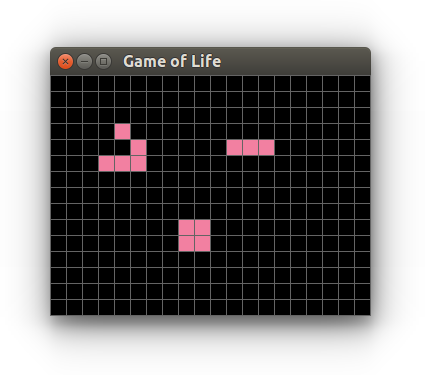
\includegraphics[width=0.8\textwidth]{../img/glider-blinker-block}

  \vspace{-2em}\caption{\label{lab:life:glider-blinker-block}Ett binärt, mörkt datauniversum av dimension $15  \times 20$. Cellkolonin innehåller tre cellgrupper: ett rymdskepp av typen \emph{glider}, en \emph{blinker} och ett \emph{block}.}
\end{figure}


\subsection{Bakgrund}

\emph{Game of Life} simulerar en koloni av encelliga organismer som lever, förökar sig och dör i en matris, enligt några enkla men väl valda regler som konstruerades av matematikern John Horton Conway på 1970-talet. Spelet går ut på att simulera flera generationer utifrån en startkonfiguration, även kallad \emph{cellkoloni}, där varje enskild cells överlevnad beror på dess omgivning. Spelet har inga medvetna spelare och om reglerna följs så kommer slutresultatet enbart bero på startkonfigurationen.

I \emph{Game of Life} består universum av en matris med celler som är antingen levande eller döda. Varje cell har 8 stycken \emph{grannar}, som utgörs av de närmsta omgivande cellerna vertikalt, horisontellt och diagonalt. Varje cells tillstånd i nästa generation bestäms av följande regler:
\begin{enumerate}[nolistsep]
    \item \textbf{Fortlevnad}. Om en levande cell har två eller tre grannar så lever den vidare.
    \item \textbf{Död}. Om en levande cell har mindre än två eller mer än tre grannar så dör den av underpopulation respektive överpopulation.
    \item \textbf{Födelse}. Om cellen är död och har exakt tre grannar så föds den och dess tillstånd ändras till levande, annars fortsätter den vara död.
\end{enumerate}

Flera cellkolonier uppvisar ett ''levande'' beteende där cellmatrisen koloniseras på intressanta vis när en sekvens av generationer visualiseras. Detta är ett exempel på \emph{emergent} beteende där komplexa, självorganiserade strukturer kan uppstå ur enkla förutsättningar.

Läs mer om \emph{Game of Life} på Wikipedia:
\begin{itemize}[noitemsep,topsep=0pt]
    	\item \url{https://en.wikipedia.org/wiki/Conway's_Game_of_Life}
    	\item \url{https://sv.wikipedia.org/wiki/Game_of_Life}
\end{itemize}


\subsection{Obligatoriska krav}

Följande funktionella krav ska uppfyllas av ditt program:
\begin{itemize}[nosep, label={$\square$},]
\item Levande celler ska ha den vackra rosa\footnote{\url{https://www.dsek.se/aktiva/grafiskprofil/farg.php}} RGB-färgen \code{(242, 128, 161)}.
\item Döda celler ska vara svarta som rymden.
\item Detta mörka universum med binära dataceller ska ritas i ett rutnät bestående av smala, stilfulla linjer, så som visas i fig. \ref{lab:life:glider-blinker-block}.
\item Tangenttryckningar och musklick ska fungera enligt följande hjälptext, som ska skrivas ut då programmet startas:
\begin{CodeSmall}
  val help = """
    Welcome to GAME OF LIFE!

    Click on cell to toggle.
    Press ENTER for next generation.
    Press SPACE to toggle play/stop.
    Press R to create random life.
    Press BACKSPACE to clear life.
    Close window to exit.
  """
\end{CodeSmall}
Då \emph{play} aktiveras med blankstegstangenten ska en kontinuerlig simulering av universum fortgå där varje ny generation visualiseras med en lagom fördröjning emellan generationer, tills simuleringen stoppas, t.ex. genom tryck ånyo på blankstegstangenten. Vid varje \emph{Enter}-tryck visas \emph{en} efterkommande generation och ev. pågående simulering stoppas. Vid musklick på en cell ska livstillståndet växlas från levande till död eller vice versa. Ett tryck på R ska ge slumpmässigt liv. Ett tryck på backstegstangenten ska rendera alla universums cellers död.

\end{itemize}

\vspace{1em}\noindent Din kod ska utformas enligt dessa design-krav:
\begin{itemize}[nosep, label={$\square$}]
\item Alla klasser och singelobjekt ska ligga i paketet \code{life}.
\item Det ska finnas en oföränderlig case-klass \code{Life} som representerar ett celluniversum med hjälp av en \code{Matrix[Boolean]} från uppgift \ref{exe:matrices:labprep} i veckans övning.
\item Det ska finnas en klass \code{LifeWindow} som visualiserar en  instans av klassen \code{Life} i ett  \code{introprog.PixelWindow} så som i fig. \ref{lab:life:glider-blinker-block}.
\end{itemize}


\subsection{Valbara krav -- välj minst ett}

Du ska implementera minst ett (gärna flera) av dessa krav:
\begin{itemize}[nosep, label={$\square$}]
\item Cellerna ska färgläggas i olika färger i enlighet med reglerna för nästa generation. Fortlevnad ska fortfarande vara vackert rosa och fortvarig död svart. Följande färger föreslås men välj andra om du tycker det blir finare:
\begin{CodeSmall}
  val UnderPopulated = java.awt.Color.cyan  // en giftig färg
  val OverPopulated  = java.awt.Color.red   // rödklämd av trängsel
  val WillBeBorn     = new java.awt.Color(40, 0, 0)  // snart levande
\end{CodeSmall}
Ge \code{LifeWindow} en klassparameter \code{isMultiColor} som styr om det blir mångfärgade celler eller om det bara finns rosa och svart som i grundkraven.

\item Om man trycker på \code{S} för \emph{Save} ska \code{introprog.Dialog.file("Save Life")} visas och, om användaren inte trycker \Button{Cancel}, det aktuella livet sparas med hjälp av \code{introprog.IO.saveString} i en textfil via metoden \code{toString} i \code{Life}.

\item Om man trycker på \code{O} för \emph{Open} ska \code{introprog.Dialog.file("Open Life")} anropas och ett nytt universum läsas in från textfil enligt lämpligt format. Inläsningen ska ske med hjälp av \code{introprog.IO.loadString} och tolkas till en \code{Life}-instans av en metod i kompanjonsobjektet med detta huvud:
\begin{CodeSmall}
def fromString(s: String, rowDelim: String="\n", alive: Char='0'): Life
\end{CodeSmall}
Testa med filen \texttt{glider-gun.txt} som ska ha följande innehåll på de första 11 raderna och totalt 32 rader där alla rader efter elfte raden innehåller tomt liv:
\begin{REPLnonum}
> head -11 glider-gun.txt
------------------------------------------
-------------------------0----------------
-----------------------0-0----------------
-------------00------00------------00-----
------------0---0----00------------00-----
-00--------0-----0---00-------------------
-00--------0---0-00----0-0----------------
-----------0-----0-------0----------------
------------0---0-------------------------
-------------00---------------------------
------------------------------------------
\end{REPLnonum}
\item Universum ska vara cirkulärt, d.v.s grannen vid kanten finns på andra sidan genom att indexeringen börjar om \Eng{wrapped} enligt modulo-räkning. Inför en klassparameter \code{isWrapped} i \code{Life} och en variabel \code{wrapped: Boolean} i kompanjonsobjektet \code{Life} som styr om fabriksmetoderna skapar ett universum som är cirkulärt eller ej, så att du lätt kan konfigurera detta. \emph{Tips:} Du har stor nytta av att använda \code|java.lang.Math.floorMod| i \code{apply}-metoden i \code{Life}; metoden \code{floorMod} räknar på lämpligt sätt med negativa värden, se dokumentationen för \code{Math}-paketet i JDK8.

\item Läs om varianter till \code{Game of Life} på Wikipedia och implementera alternativa regler som görs valbara genom konfigurering via \code{args}-parametern i \code{main}.

\item Skapa en klass \code{LifeStatistics} som genom väldigt många simuleringar ska ta reda på sannolikheten att en slumpmässig cellkoloni efter $n$ generationer fortfarande utvecklas, respektive är helt dött. Ingen visualisering med \code{PixelWindow} ska ske; endast antalet celler som lever vid generation $n$ och antalet celler som ändrades sedan generation $n - 1$ behöver registreras.

\end{itemize}




\subsection{Tips och förslag}

\begin{enumerate}[leftmargin=*]
\item Här är ett förslag på hur du kan utforma klassen \code{Life}:
\begin{CodeSmall}
package life

case class Life(val cells: Matrix[Boolean]) {

  /** Ger true om cellen på plats (row, col) är vid liv annars false.
    * Ger false om indexeringen är utanför universums gränser.
    */
  def apply(row: Int, col: Int): Boolean = ???

  /** Sätter status på cellen på plats (row, col) till value. */
  def updated(row: Int, col: Int, value: Boolean): Life = ???

  /** Växlar status på cellen på plats (row, col). */
  def toggled(row: Int, col: Int): Life = ???

  /** Räknar antalet levande grannar till cellen i (row, col).*/
  def nbrOfNeighbours(row: Int, col: Int): Int = ???

  /** Skapar en ny Life-instans med nästa generation av universum.
    * Detta sker genom att applicera funktionen \code{rule} på cellerna.
    */
  def evolved(rule: (Int, Int, Life) => Boolean = Life.defaultRule):Life = {
    var nextGeneration = Life.empty(cells.dim)
    cells.foreachIndex { (r,c) =>
      ???
    }
    nextGeneration
  }

  override def toString =
    cells.data.map(_.map(if (_) '0' else '-').mkString).mkString("\n")
}

object Life {
  /** Skapar ett universum med döda celler. */
  def empty(dim: (Int, Int)): Life = ???

  /** Skapar ett unviversum med slumpmässigt liv. */
  def random(dim: (Int, Int)): Life = ???

  /** Implementerar reglerna enligt Conways Game of Life. */
  def defaultRule(row: Int, col: Int, current: Life): Boolean = ???
}
\end{CodeSmall}
Du har nytta av metoden \code{copy} när du implementerar \code{updated} och \code{toggled}. Metoden \code{nbrOfNeighbours} har du nytta av när du ska implementera \code{defaultRule}. När du ska implementera \code{random} har du nytta av metoden \code{foreachIndex} i \code{Matrix[T]}.
Om du som i förslaget ovan låter \code{evolved} ta uppdateringsregeln som en funktionsparameter blir det lättare att konfigurera vilka regler som ska gälla och därmed blir det även lättare att skapa varianter av \emph{Game of Life} genom att införa nya regler i kompanjonsobjektet (se en av de valfria uppgifterna med vidare hänvisning till Wikipedia).

\item Här är ett förslag på hur du kan utforma klassen \code{LifeWindow}:
\begin{CodeSmall}
package life

import introprog.PixelWindow
import introprog.PixelWindow.Event

class LifeWindow(rows: Int, cols: Int){
  import LifeWindow._ // importera konstanter för cellstorlek, färger, etc.

  var life = Life.empty(rows, cols)
  val window: PixelWindow = ???
  var quit = false
  var play = false

  def drawGrid(): Unit = ???

  def drawCell(row: Int, col: Int): Unit = ???

  def update(newLife: Life): Unit = {
    val oldLife = life
    life = newLife
    life.cells.foreachIndex{ ??? }
  }

  def handleKey(key: String): Unit = ???

  def handleClick(pos: (Int, Int)): Unit = ???

  def loopUntilQuit(): Unit = while (!quit) {
    val t0 = System.currentTimeMillis
    if (play) update(life.evolved())
    window.awaitEvent(EventMaxWait)
    while (window.lastEventType != PixelWindow.Event.Undefined) {
      window.lastEventType match {
        case Event.KeyPressed  =>  handleKey(window.lastKey)
        case Event.MousePressed => handleClick(window.lastMousePos)
        case Event.WindowClosed => quit = true
        case _ =>
      }
      window.awaitEvent(EventMaxWait)
    }
    val elapsed = System.currentTimeMillis - t0
    Thread.sleep((NextGenerationDelay - elapsed) max 0)
  }

  def start(): Unit = { drawGrid(); loopUntilQuit() }
}
\end{CodeSmall}

\item \textbf{Dra nytta av den IDE du valt.} Det finns många användbara finesser i en integrerad utvecklingsmiljö. Orientera dig om grunderna genom att läsa appendix \ref{appendix:ide}. Lär dig några viktiga kortkommandon och studera hur du får igång debuggern. Prova att i debuggern sätta brytpunkter, stega dig fram och avläsa variablers värden.
\end{enumerate}

\noindent\TODO Är det för mycket tips? Eller behövs mer tips för att labben ska gå smidigt?


%!TEX encoding = UTF-8 Unicode

%!TEX root = ../compendium2.tex

\chapter{Arv, Gränssnitt}
\begin{itemize}[nosep]
\item klasser
\item arv
\item polymorfism
\item likhet
\item equals
\item accessregler
\item private
\item public
\item protected
\item private[this]
\item trait
\item inmixning
\item Any
\item AnyVal
\item AnyRef
\item Nothing\end{itemize}
\newpage


%!TEX encoding = UTF-8 Unicode
%!TEX root = ../exercises.tex

\ifPreSolution

\Exercise{\ExeWeekNINE}\label{exe:W09}

\begin{Goals}
%!TEX encoding = UTF-8 Unicode

%!TEX root = ../compendium2.tex

\item Förstå följande begrepp: supertyp, subtyp, bastyp, abstrakt typ, polymorfism.
\item Kunna deklarera och använda en arvshierarki i flera nivåer med nyckelordet \code{extends}.
\item Kunna deklarera och använda inmixning med flera traits och nyckelordet \code{with}.
\item Kunna deklarera och känna till nyttan med finala klasser och finala attribut och nyckelordet \code{final}.
\item Känna till synlighetsregler vid arv och nyttan med privata och skyddade attribut.
\item Kunna deklarera och använda skyddade attribut med nyckelordet \code{protected}.
\item Känna till hur typtester och typkonvertering vid arv kan göras med metoderna \code{isInstanceOf} och \code{asInstanceOf} och känna till att detta görs bättre med \code{match}.
\item Känna till begreppet anonym klass.
\item Kunna deklarera och använda överskuggade metoder med nyckelordet \code{override}.
\item Känna till reglerna som gäller vid överskuggning av olika sorters medlemmar.
\item Kunna deklarera och använda hierarkier av klasser där konstruktorparametrar överförs till superklasser.
\item Kunna deklarera och använda uppräknade värden med case-objekt och gemensam bastyp.

\end{Goals}

\begin{Preparations}
\item \StudyTheory{09}
\end{Preparations}

\BasicTasks

\else

\ExerciseSolution{\ExeWeekNINE}

\BasicTasks

\fi



\WHAT{Para ihop begrepp med beskrivning.}

\QUESTBEGIN

\Task \what

\vspace{1em}\noindent Koppla varje begrepp med den (förenklade) beskrivning som passar bäst:

\begin{ConceptConnections}
  bastyp & 1 & & A & körtidstypen avgör vilken metod som körs \\ 
  supertyp & 2 & & B & minneslagring kan optimeras, har supertypen \code|AnyVal| \\ 
  subtyp & 3 & & C & klass utan namn, utvidgad med extra implementation \\ 
  körtidstyp & 4 & & D & är endast synlig i subtyper \\ 
  dynamisk bindning & 5 & & E & kan ej instansieras \\ 
  polymorfism & 6 & & F & abstrakt klass, kan mixas in, kan ej ha parametrar \\ 
  trait & 7 & & G & saknar implementation \\ 
  inmixning & 8 & & H & kan vara mer specifik än den statiska typen \\ 
  överskuggad medlem & 9 & & I & ej värdetyp, har supertypen \code|AnyRef| \\ 
  anonym klass & 10 & & J & kan ha många former, t.ex. en av flera subtyper \\ 
  skyddad medlem & 11 & & K & subtypning utanför denna kodfil är förhindrad \\ 
  abstrakt medlem & 12 & & L & medlem i subtyp ersätter medlem i supertyp \\ 
  abstrakt klass & 13 & & M & en typ som är mer specifik \\ 
  referenstyp & 14 & & N & en typ som är mer generell \\ 
  förseglad typ & 15 & & O & klass får nya egenskaper från trait \\ 
  värdetyp & 16 & & P & den mest generella typen i en arvshierarki \\ 
\end{ConceptConnections}

\SOLUTION

\TaskSolved \what

\begin{ConceptConnections}
  bastyp & 1 & ~~\Large$\leadsto$~~ &  P & den mest generella typen i en arvshierarki \\ 
  sypertyp & 2 & ~~\Large$\leadsto$~~ &  N & en typ som är mer generell \\ 
  subtyp & 3 & ~~\Large$\leadsto$~~ &  M & en typ som är mer specifik \\ 
  körtidstyp & 4 & ~~\Large$\leadsto$~~ &  H & kan vara mer specifik än den statiska typen \\ 
  dynamisk bindning & 5 & ~~\Large$\leadsto$~~ &  A & körtidstypen avgör vilken metod som körs \\ 
  plymorfism & 6 & ~~\Large$\leadsto$~~ &  J & kan ha många former, t.ex. en av flera subtyper \\ 
  trait & 7 & ~~\Large$\leadsto$~~ &  F & abstrakt klass, kan mixas in, kan ej ha parametrar \\ 
  inmixning & 8 & ~~\Large$\leadsto$~~ &  O & klass får nya egenskaper från trait \\ 
  överskuggad medlem & 9 & ~~\Large$\leadsto$~~ &  L & medlem i subtyp ersätter medlem i supertyp \\ 
  anonym klass & 10 & ~~\Large$\leadsto$~~ &  C & den mest generella typen i en arvshierarki \\ 
  skyddad medlem & 11 & ~~\Large$\leadsto$~~ &  D & är endast synlig i subtyper \\ 
  abstrakt medlem & 12 & ~~\Large$\leadsto$~~ &  G & saknar implementation \\ 
  abstrakt klass & 13 & ~~\Large$\leadsto$~~ &  E & kan ej instansieras \\ 
  referenstyp & 14 & ~~\Large$\leadsto$~~ &  I & ej värdetyp, har supertypen \code|AnyRef| \\ 
  förseglad typ & 15 & ~~\Large$\leadsto$~~ &  K & subtypning utanför denna kodfil är förhindrad \\ 
  värdetyp & 16 & ~~\Large$\leadsto$~~ &  B & minneslagring kan optimeras, har supertypen, \code|AnyVal| \\ 
\end{ConceptConnections}

\QUESTEND





\WHAT{Gemensam bastyp.}

\QUESTBEGIN

\Task  \what~  Man vill ofta lägga in objekt av olika typ i samma samling.
\begin{REPL}
scala> class Gurka(val vikt: Int)
scala> class Tomat(val vikt: Int)
scala> val gurkor = Vector(new Gurka(100), new Gurka(200))
scala> val grönsaker = Vector(new Gurka(300), new Tomat(42))
\end{REPL}
\Subtask Om en samling innehåller objekt av flera olika typer försöker kompilatorn härleda den mest specifika typen som objekten har gemensamt. Vad blir det för typ på värdet \code{grönsaker} ovan?

\Subtask Försök ta reda på summan av vikterna enligt nedan. Vad ger andra raden för felmeddelande? Varför?

\begin{REPL}
scala> gurkor.map(_.vikt).sum
scala> grönsaker.map(_.vikt).sum
\end{REPL}

\Subtask Vi kan göra så att vi kan komma åt vikten på alla grönsaker genom att ge gurkor och tomater en gemensam bastyp som de olika konkreta grönsakstyperna utvidgar med nyckelordet \code{extends}. Man säger att subtyperna \code{Gurka} och \code{Tomat} \textbf{ärver} egenskaperna hos supertypen \code{Grönsak}.

Attributet \code{vikt} i traiten \code{Grönsak} nedan initialiseras inte förrän konstruktorerna anropas när vi gör \code{new} på någon av klasserna \code{Gurka} eller \code{Tomat}.

\begin{REPL}
scala> trait Grönsak { val vikt: Int }
scala> class Gurka(val vikt: Int) extends Grönsak
scala> class Tomat(val vikt: Int) extends Grönsak
scala> val gurkor = Vector(new Gurka(100), new Gurka(200))
scala> val grönsaker = Vector(new Gurka(300), new Tomat(42))
\end{REPL}

\Subtask Vad blir det nu för typ på variabeln \code{grönsaker} ovan?

\Subtask Undersök om det nu går att räkna ut summan av vikterna i \code{grönsaker} med \\ \code{grönsaker.map(_.vikt).sum}


\Subtask En trait liknar en klass, men man kan inte instansiera den och den kan inte ha några parametrar. En typ som inte kan instansieras kallas \textbf{abstrakt} \Eng{abstract}. Vad blir det för felmeddelande om du försöker göra \code{new} på en trait enligt nedan?
\begin{REPL}
scala> trait Grönsak { val vikt: Int }
scala> new Grönsak
\end{REPL}


\Subtask Traiten \code{Grönsak} har en abstrakt medlem \code{vikt}. Den sägs vara abstrakt eftersom den saknar definition -- medlemmen har bara ett namn och en typ men inget värde. Du kan instansiera den abstrakta traiten \code{Grönsak} om du fyller i det som ''fattas'', nämligen ett värde på \code{vikt}. Man kan fylla på det som fattas i genom att ''hänga på'' ett block efter typens namn vid instansiering. Man får då vad som kallas en \textbf{anonym} klass, i detta fall en ganska konstig grönsak som inte är någon speciell sorts grönsak med som ändå har en vikt.

Vad får \code{anonymGrönsak} nedan för typ och strängrepresenation?
\begin{REPL}
scala> val anonymGrönsak = new Grönsak { val vikt = 42 }
\end{REPL}



\SOLUTION


\TaskSolved \what


\SubtaskSolved  \code{Vector[Object]}.

\SubtaskSolved  Det beror på att vektorns element är av typen \code{Object}. \code{vikt} är inte definierat för denna typ.

\SubtaskSolved  -.

\SubtaskSolved  \code{Vector[Grönsak]}.

\SubtaskSolved  Ja.

\SubtaskSolved  -.

\SubtaskSolved  \code{Grönsak}. \$anon\$1@88dfbe.


\QUESTEND






\WHAT{Polymorfism i samband med arv.}

\QUESTBEGIN

\Task  \what~  Polymorfism betyder ''många skepnader''. I samband med arv  innebär det att flera subtyper, till exempel \code{Ko} och \code{Gris}, kan hanteras gemensamt som om de vore instanser av samma supertyp, så som \code{Djur}. Subklasser kan implementera en metod med samma namn på olika sätt. Vilken metod som exekveras bestäms vid körtid beroende på vilken subtyp som instansieras. På så sätt kan djur komma i många skepnader.

\Subtask Implementera funktionen \code{skapaDjur} nedan så att den returnerar antingen en ny Ko eller en ny Gris med lika sannolikhet.

\begin{REPL}
scala> trait Djur { def väsnas: Unit }
scala> class Ko   extends Djur { def väsnas = println("Muuuuuuu") }
scala> class Gris extends Djur { def väsnas = println("Nöffnöff") }
scala> def skapaDjur: Djur = ???
scala> val bondgård = Vector.fill(42)(skapaDjur)
scala> bondgård.foreach(_.väsnas)
\end{REPL}

\Subtask Lägg till ett djur av typen Häst som väsnas på lämpligt sätt och modifiera \code{skapaDjur} så att det skapas kor, grisar och hästar med lika sannolikhet.



\SOLUTION


\TaskSolved \what


\SubtaskSolved
\begin{Code}
def skapaDjur: Djur =
   {if(math.random > 0.5) new Ko else new Gris}
\end{Code}

\SubtaskSolved
\begin{Code}
class Häst extends Djur{ def väsnas = println("Gnääääägg") }
def skapaDjur: Djur = {val r = math.random;
   if(r < 0.33) new Ko else if(r < 0.67) new Gris else new Häst}
\end{Code}


\QUESTEND









\WHAT{Supertyp med parameter.}

\QUESTBEGIN

\Task  \what~  En trait kan inte ha någon parameter. Vill man ha en parameter till supertypen måste man använda en klass istället, enligt nedan exempel.

Utbildningsdepartementet vill i sitt system hålla koll på vissa personer och skapar därför en klasshierarki enligt nedan. Skriv in koden i en editor och klipp sedan in den i REPL.
\begin{Code}
class Person(val namn: String)

class Akademiker(
  namn: String,
  val universitet: String) extends Person(namn)

class Student(
  namn: String,
  universitet: String,
  program: String) extends Akademiker(namn, universitet)

class Forskare(
  namn: String,
  universitet: String,
  titel: String) extends Akademiker(namn, universitet)
\end{Code}


\Subtask Deklarera fyra olika \code{val}-variabler med lämpliga namn som refererar till olika instanser av alla olika klasser ovan och ge attributen valfria initialvärden genom olika parametrar till konstruktorerna.

\Subtask Skriv två satser: en som först stoppar in instanserna i en \code{Vector} och en som sedan loopar igenom vektorn och skriv ut alla instansers \code{toString} och \code{namn}.


\Subtask Utbildningsdepartementet vill att det inte ska gå att instansiera objekt av typerna \code{Person} och \code{Akademiker}. Det kan åstadkommas genom att placera nyckelordet \code{abstract} före \code{class}. Uppdatera koden i enlighet med detta. Vilket blir felmeddelande om man försöker instansiera en \code{abstract class}?

\Subtask Utbildningsdeparetementet vill slippa implementera \code{toString} och slippa skriva \code{new} vid instansiering. Gör därför om typerna \code{Student} och \code{Forskare} till case-klasser. \emph{Tips:} För att undkomma ett kompileringsfel (vilket?) behöver du använda \code{override val} på lämpligt ställe.

Skapa instanser av de nya case-klasserna \code{Student} och \code{Forskare} och skriv ut deras \code{toString}. Hur ser utskriften ut?

\Subtask Eftersom \code{Person} och \code{Akademiker} nu är abstrakta, vill utbildningsdepartementet att du gör om dessa typer till traits med abstrakta attribut istället för klasser. Du kan då undvika \code{override val} i klassparametrarna till de konkreta case-klasserna.

Man inför också en case-klass \code{IckeAkademiker} som man tänker använda i olika statistiska medborgarundersökningar.

Dessutom förser man alla personer med ett personnummer representerat som en \code{Long}.

Hur ser utbildningsdepartementets kod ut nu, efter alla ändringar? Skriv ett testprogram som skapar några instanser och skriver ut deras attribut.

\Subtask I vilka sammanhang är det nödvändigt att använda en \code{trait} respektive en \code{class}?

\SOLUTION


\TaskSolved \what


\SubtaskSolved
\begin{Code}
val person = new Person("Person1")
val akademiker = new Akademiker("Person2", "LTH")
val student = new Student("Person3", "LTH", "D")
val forskare = new Forskare("Person4", "LTH", "Doktorand")
\end{Code}

\SubtaskSolved
\begin{Code}
val vec = Vector(person, akademiker, student, forskare)
for(i <- vec){ print(i.toString + i.namn) }
\end{Code}

\SubtaskSolved  error: class Person is abstract; cannot be instantiated.

\SubtaskSolved  error: overriding value namn in class Person of type String; value namn needs `override' modifier.\\
toString för Student: Student(Person3,LTH,D). \\
toString för Forskare: Student(Person4,LTH,Doktorand).

\SubtaskSolved
\begin{Code}
trait Person {val namn: String; val nbr: Long}
trait Akademiker extends Person {val universitet: String}
case class Student(
  namn: String,
  nbr: Long,
  universitet: String,
  program: String) extends Akademiker
case class Forskare(
  namn: String,
  nbr: Long,
  universitet: String,
  titel: String) extends Akademiker
case class IckeAkademiker(
    namn: String,
    nbr: Long) extends Person
\end{Code}

\SubtaskSolved  Man måste använda en klass om man behöver klassparametrar. Man måste använda en trait om man vill göra in-mixning med \code{with}. \\
 Se \href{http://www.artima.com/pins1ed/traits.html\#12.7}{http://www.artima.com/pins1ed/traits.html\#12.7}.


\QUESTEND








\WHAT{Uppräknade värden.}

\QUESTBEGIN

\Task  \what~  Ett sätt att hålla reda på uppräknade värden, t.ex. färgen på olika kort i en kortlek, är att använda olika heltal som får representera de olika värdena, till exempel så här:\footnote{Om namnkonventioner för konstanter i Scala: läs under rubriken ''Constants, Values, Variable and Methods'' här \href{http://docs.scala-lang.org/style/naming-conventions.html}{docs.scala-lang.org/style/naming-conventions.html}}
\begin{Code}
object Färg {
  val Spader = 1
  val Hjärter = 2
  val Ruter = 3
  val Klöver = 4
}
\end{Code}
Dessa kan sedan användas som parametrar till denna case-klass vid skapande av kortobjekt:
\begin{lstlisting}[language=,keywords={case,class}]
case class Kort(färg: Int, valör: Int)
\end{lstlisting}
Man kan hålla reda på färgen med en variabel av typen \code{Int} och tilldela den en viss färg med ovan konstanter. Och när man skapar ett kort behöver man inte komma ihåg vilket numret är.
\begin{REPL}
scala> val f = Färg.Spader
scala> import Färg._
scala> Kort(Ruter, 7)
\end{REPL}
En annan fördelen med detta är att man lätt kan loopa från 1 till 4 för att gå igenom alla färger.
\begin{REPL}
scala> val kortlek = for (f <- 1 to 4; v <- 1 to 13) yield Kort(f, v)
\end{REPL}
Nackdelen är att kompilatorn vid kompileringstid inte kollar om variablerna av misstag råkar ges något värde utanför det giltiga intervallet, t.ex. 42. Detta får vi själv hålla koll på vid körtid, till exempel med funktionen \code{require} eller \code{if}-satser, etc.

Istället kan man använda case-objekt enligt nedan deluppgifter och få hjälp av kompilatorn att hitta eventuella fel vid kompileringstid.  Ett case-objekt är som ett vanligt singelton-objekt men det får automatiskt en \code{toString} samma som namnet och kan användas i matchningar etc. (mer om match i kapitel \ref{chapter:W08}).

\Subtask Deklarera följande uppräknade värden som singelton objekt med gemensam bastyp. Med nyckelordet \code{sealed} så ''förseglas'' klassen och inga andra direkta subtyper tillåts förutom de som finns i samma kod-fil eller block. I detta exempel  med kortfärger vet vi ju att det inte finns fler än dessa fyra färger.
\begin{Code}
sealed trait Färg
case object Spader extends Färg
case object Hjärter extends Färg
case object Ruter extends Färg
case object Klöver extends Färg
\end{Code}
Dessa kan sedan användas som parametrar till denna case-klass vid skapande av kortobjekt:
\begin{lstlisting}[language=,keywords={case,class}]
case class Kort(färg: Färg, valör: Int)
\end{lstlisting}
Skapa därefter några exempelinstanser av klassen \code{Kort}. Vad är fördelen med ovan angreppssätt jämfört med att använda heltalskonstanter?

\Subtask Om man vill kunna iterera över alla värden är det bra om de finns i en samling med alla värden. Vi kan lägga en sådan i ett kompanjonsobjekt till bastypen enligt nedan. Skriv ut alla färgvärden med en \code{for}-sats.

\begin{Code}
sealed trait Färg
object Färg {
  val values = Vector(Spader, Hjärter, Ruter, Klöver)
}
case object Spader extends Färg
case object Hjärter extends Färg
case object Ruter extends Färg
case object Klöver extends Färg
\end{Code}
Skapa en kortlek med 52 olika kort och blanda den sedan med \code{Random.shuffle} enligt nedan. Använd en dubbel \code{for}-sats och \code{yield}.
\begin{REPL}
scala> val kortlek: Vector[Kort] = ???
scala> val blandad = scala.util.Random.shuffle(kortlek)
\end{REPL}

\Subtask Skriv en funktion \code{ def blandadKortlek: Vector[Kort] = ???} som ger en ny blandad kortlek varje gång den anropas med metoden i föregående uppgift.

%%%%%%%%%%%%%%%%%%% FEEEEEELLL \end{Code}



\Subtask Om man även vill ha en heltalsrepresentation med en medlem \code{toInt} för alla värden, kan man ge bastypen en parameter och i stället för en trait (som inte kan ha några parametrar) använda en abstrakt klass.

\begin{Code}
sealed abstract class Färg(final val toInt: Int)
object Färg {
  val values = Vector(Spader, Hjärter, Ruter, Klöver)
}
case object Spader  extends Färg(0)
case object Hjärter extends Färg(1)
case object Ruter   extends Färg(2)
case object Klöver  extends Färg(3)
\end{Code}
Skapa en funktion \code{färgPoäng} som räknar ut summan av heltalsrepresentationen av alla färger hos en vektor med kort, och använd den sedan för att räkna ut \code{färgPoäng} för de första fem korten.
\begin{REPL}
scala> def blandadKortlek: Vector[Kort] = ???
scala> def färgPoäng(xs: Vector[Kort]): Int = ???
scala> färgPoäng(blandadKortlek.take(5))
\end{REPL}


\SOLUTION

\TaskSolved \what

\SubtaskSolved  Sättet är säkrare då man inte kan tilldela korten en färg som inte finns. Med heltalskonstanterna kan man till exempel ge ett kort färgen 5, vilken inte korresponderar till någon riktig färg.

\SubtaskSolved  \code{for (f <- Färg.values; v <- 1 to 13) yield Kort(f,v)}

\SubtaskSolved
\begin{Code}
def blandadKortlek: Vector[Kort] = {
  val kortlek =
    for (f <- Färg.values; v <- 1 to 13) yield Kort(f,v)
  scala.util.Random.shuffle(kortlek)
}
\end{Code}

\SubtaskSolved  \code{def färgPoäng(xs: Vector[Kort]): Int = xs.map(_.färg.toInt).sum}

\QUESTEND












\ExtraTasks %%%%%%%%%%%%%%%%%



\WHAT{Bastypen \code{Shape} och subtyperna \code{Rectangle} och \code{Circle}.}

\QUESTBEGIN

\Task  \what~  Du ska i denna uppgift skapa ett litet bibliotek för geometriska former med oföränderliga objekt implementerade med hjälp av case-klasser. De geometriska formerna har en gemensam bastyp kallad \code{Shape}. Utgå från koden nedan.

\begin{Code}
case class Point(x: Double, y: Double) {
  def move(dx: Double, dy: Double): Point = Point(x + dx, y + dy)
}

trait Shape {
  def pos: Point
  def move(dx: Double, dy: Double): Shape
}

case class Rectangle(
  pos: Point,
  dx: Double,
  dy: Double
) extends Shape {
  override def move(dx: Double, dy: Double): Rectangle =
    Rectangle(pos.move(dx, dy), this.dx, this.dy)
}

case class Circle(pos: Point, radius: Double) extends Shape {
  override def move(dx: Double, dy: Double): Circle =
    Circle(pos.move(dx, dy), radius)
}
\end{Code}

\Subtask Instansiera några cirklar och rektanglar och gör några relativa förflyttningar av dina instanser genom att anropa \code{move}.

\Subtask Lägg till metoden \code{moveTo} i \code{Point}, \code{Shape}, \code{Rectangle} och \code{Circle} som gör en absolut förflyttning till koordinaterna \code{x} och \code{y}. Testa med REPL på några instanser av \code{Rectangle} och \code{Circle}.

\Subtask Lägg till metoden \code{distanceTo(that: Point): Double } i case-klassen \code{Point} som räknar ut avståndet till en annan punkt med hjälp av \code{math.hypot}. Klistra in i REPL och testa på några instanser av \code{Point}.

\Subtask Lägg till en konkret metod \code{distanceTo(that: Shape): Double } i traiten \code{Shape} som räknar ut avståndet till positionen för en annan Shape. Testa i REPL på några instanser av \code{Rectangle} och \code{Circle}.

\SOLUTION


\TaskSolved \what


\SubtaskSolved
\begin{Code}
val c1 = Circle(Point(1, 1), 42)
val r1 = Rectangle(Point(3, 3), 20, 30)
c1.move(2, 3)
r1.move(3, 2)
\end{Code}

\SubtaskSolved  För \code{Point}: \code{def moveTo(dx: Double, dy: Double): Point = Point(dx, dy)}. \\
För \code{Shape}: \code{def moveTo(dx: Double, dy: Double): Shape}. \\
För \code{Rectangle}: \code{override def moveTo(dx: Double, dy: Double): Rectangle = } \\
\code{Rectangle(pos.moveTo(dx, dy), this.dx, this.dy)}. \\
För \code{Circle}: \code{override def moveTo(dx: Double, dy: Double): Circle =} \\
\code{Circle(pos.moveTo(dx, dy), radius)}.

\SubtaskSolved  \code{def distanceTo(that: Point): Double = math.hypot(that.x - x, that.y - y)}.

\SubtaskSolved  \code{def distanceTo(that: Shape): Double = pos.distanceTo(that.pos)}.


\QUESTEND






\WHAT{Regler för \code{override}, \code{private} och \code{final}.}

\QUESTBEGIN

\Task  \what~

\Subtask \label{subtask:overriderules} Undersök överskuggningning av abstrakta, konkreta, privata och finala medlemmar genom att skriva in raderna nedan en i taget i REPL. Vilka rader ger felmeddelande? Varför? Vid felmeddelande: notera hur felmeddelandet lyder och ändra deklarationen av den felande medlemmen så att koden blir kompilerbar (eller om det är enda rimliga lösningen: ta bort den felaktiga medlemmen), innan du provar efterkommande rad.

\begin{REPL}
trait Super1 { def a: Int; def b = 42; private def c = "hemlis" }
class Sub2 extends Super1 { def a = 43; def b = 43; def c = 43 }
class Sub3 extends Super1 { def a = 43; override def b = 43 }
class Sub4 extends Super1 { def a = 43; override def c = "43" }
trait Super5 { final def a: Int; final def b = 42 }
class Sub6 extends Super5 { override def a = 43; def b = 43 }
class Sub7 extends Super5 { def a = 43; override def b = 43 }
class Sub8 extends Super5 { def a = 43; override def c = "43" }
trait Super9 { val a: Int; val b = 42; lazy val c: String = "lazy" }
class Sub10 extends Super9 { override def a = 43; override val b = 43 }
class Sub11 extends Super9 { val a = 43; override lazy val b = 43 }
class Sub12 extends Super9 { val a = 43; override var b = 43 }
class Sub13 extends Super9 { val a = 43; override lazy val c = "still lazy" }
class SubSub extends Sub13 { override val a = 44}
trait Super14 { var a: Int; var b = 42; var c: String }
class Sub15 extends Super14 { def a = 43; override var b = 43; val c = "?" }
\end{REPL}

\Subtask Skapa instanser av klasserna \code{Sub3}, \code{Sub13} och \code{SubSub} från ovan deluppgift och undersök alla medlemmarnas värden för respektive instans. Förklara varför de har dessa värden.

%\Subtask Läs igenom reglerna i kapitel  \ref{slideW07:overriderules} om vad som gäller vid arv och överskuggning av medlemmar. Gör några egna undersökningar i REPL som försöker bryta mot någon regel som inte testades i deluppgift \ref{subtask:overriderules}.

\SOLUTION


\TaskSolved \what


\SubtaskSolved  2. Måste ha \code{override} framför \code{b} för att kunna ändra på metoden. \\
4. \code{c} är \code{private}, vilket betyder att den är gömd för subklasserna. Därför kan den inte överskuggas. Genom att ta bort \code{override} fungerar klassen. \\
5. En \code{final}-medlem måste ha ett bestämt värde. Kan lösas genom att tilldela \code{final a} ett värde eller ta bort \code{final}. \\
6. En \code{final}-medlem kan inte överskuggas, varken med eller utan \code{override}. Här får konflikterna tas bort.  \\
7. Se 6. \\
8. Eftersom \code{c} inte finns i \code{Super5} kan den inte överskuggas. Genom att ta bort \code{override} fungerar klassen. \\
10. Överskuggningen av \code{val} måste vara oföränderlig (immutable); detta är inte nödvändigtvis \code{def}. Löses genom att byta ut \code{def a} mot \code{val a} hos \code{Sub10}.  \\
11. Samma problem som i 10.; \code{lazy val} kan vara föränderlig. Löses genom att ta bort \code{lazy}. \\
12. Samma problem igen! \code{var} är föränderlig, vilket bryter mot typsäkerheten när man försöker överskugga en \code{val}. Löses genom att ändra \code{var} till \code{val}. \\
15.\code{def a = 43} och \code{val c = "?"} täcker inte allt som \code{var} kräver. Det behövs en setter för att kunna uppfylla kraven för överskuggning för en \code{var}. Dessutom finns det ingen anledning för en \code{val} att överskuggas; man kan ju ändra på den lite hur man vill!

\SubtaskSolved  Sub3: a = 43, b = 43 eftersom medlemmen är överskuggad. c hittas inte eftersom den är \code{private}.

Sub13: a = 43, b = 42, c = "still lazy" eftersom medlemmen överskuggas.

SubSub: a = 44 eftersom medlemmen överskuggas, b = 42, c = "still lazy".

\SubtaskSolved  -.


\QUESTEND





\AdvancedTasks %%%%%%%%%%%%%%%%%




\WHAT{Inmixning.}

\QUESTBEGIN

\Task \label{task:fyle} \what~   Man kan utvidga en klass med multipla traits med nyckelordet \code{with}. På så sätt kan man fördela medlemmar i olika traits och återanvända gemensamma koddelar genom så kallad \textbf{inmixning}, så som nedan exempel visar.

En alternativ fågeltaxonomi, speciellt populär i Skåne, delar in alla fåglar i två specifika kategorier: Kråga respektive Ånka. Krågor kan flyga men inte simma, medan Ånkor kan simma och oftast även flyga. Fågel i generell, kollektiv bemärkelse kallas på gammal skånska för Fyle.%
\footnote{\href{http://www.klangfix.se/ordlista.htm}{www.klangfix.se/ordlista.htm}}

\begin{Code}
trait Fyle {
  val läte: String
  def väsnas: Unit = print(läte * 2)
  val ärSimkunnig: Boolean
  val ärFlygkunnig: Boolean
}

trait KanSimma       { val ärSimkunnig = true }
trait KanInteSimma   { val ärSimkunnig = false }
trait KanFlyga       { val ärFlygkunnig = true }
trait KanKanskeFlyga { val ärFlygkunnig = math.random < 0.8 }

class Kråga extends Fyle with KanFlyga with KanInteSimma {
  val läte = "krax"
}

class Ånka extends Fyle with KanSimma with KanKanskeFlyga {
  val läte = "kvack"
  override def väsnas = print(läte * 4)
}
\end{Code}

\Subtask En flitig ornitolog hittar 42 fåglar i en perfekt skog där alla fågelsorter är lika sannolika, representerat av vektorn \code{fyle} nedan. Skriv i REPL ett uttryck som undersöker hur många av dessa som är flygkunniga Ånkor, genom att använda metoderna \code{filter}, \code{isInstanceOf}, \code{ärFlygkunnig} och \code{size}.

\begin{REPL}
scala> val fyle =
         Vector.fill(42)(if (math.random > 0.5) new Kråga else new Ånka)
scala> fyle.foreach(_.väsnas)
scala> val antalFlygånkor: Int = ???
\end{REPL}

\Subtask \label{subtask:fyle:sound} Om alla de fåglar som ornitologen hittade skulle väsnas exakt en gång var, hur många krax och hur många kvack skulle då höras? Använd metoderna \code{filter} och \code{size}, samt predikatet \code{ärSimkunnig} för att beräkna antalet krax respektive kvack.
\begin{REPL}
scala> val antalKrax: Int = ???
scala> val antalKvack: Int = ???
\end{REPL}

\SOLUTION


\TaskSolved \what


\SubtaskSolved
\begin{Code}
fyle.filter(f => f.isInstanceOf[Ånka] && f.ärFlygkunnig).size
\end{Code}

\SubtaskSolved
\begin{Code}
val antalKrax: Int = fyle.filter(f => !f.ärSimkunnig).size * 2
val antalKvack: Int = fyle.filter(f => f.ärSimkunnig).size * 4
\end{Code}


\QUESTEND











\WHAT{Finala klasser.}

\QUESTBEGIN

\Task  \what~  Om man vill förhindra att man kan göra \code{extends} på en klass kan man göra den final genom att placera nyckelordet \code{final} före nyckelordet \code{class}.

\Subtask Eftersom klassificeringen av fåglar i uppgiften ovan i antingen Ånkor eller Krågor är fullständig och det inte finns några subtyper till varken Ånkor eller Krågor är det lämpligt att göra dessa finala. Ändra detta i din kod.

\Subtask Testa att ändå försöka göra en subklass \code{Simkråga extends Kråga}. Vad ger kompilatorn för felmeddelande om man försöker utvidga en final klass?


\SOLUTION


\TaskSolved \what


\SubtaskSolved  Sätt \code{final} framför \code{class} i klasserna.

\SubtaskSolved  error: illegal inheritance from final class Kråga.


\QUESTEND






\WHAT{Accessregler vid arv och nyckelordet \code{protected}.}

\QUESTBEGIN

\Task  \what~  Om en medlem i en supertyp är privat så kan man inte komma åt den i en subklass. Ibland vill man att subklassen ska kunna komma åt en medlem även om den ska vara otillgänglig i annan kod.

\begin{REPL}
trait Super {
  private val minHemlis = 42
  protected val vårHemlis = 42
}
class Sub extends Super {
  def avslöja = minHemlis
  def kryptisk = vårHemlis * math.Pi
}
\end{REPL}

\Subtask Vad blir felmeddelandet när klassen \code{Sub} försöker komma åt \code{minHemlis}?

\Subtask Deklarera \code{Sub} på nytt, men nu utan den förbjudna metoden \code{avslöja}. Vad blir felmeddelandet om du försöker komma åt \code{vårHemlis} via en instans av klassen \code{Sub}? Prova till exempel med \code{(new Sub).vårHemlis}

\Subtask Fungerar det att anropa metoden \code{kryptisk} på instanser av klassen \code{Sub}?

\SOLUTION


\TaskSolved \what


\SubtaskSolved  error: not found: value minHemlis.

\SubtaskSolved  error: value vårHemlis in class Super\$class cannot be accessed in Sub.

\SubtaskSolved  Ja.


\QUESTEND






\WHAT{Använding av \code{protected}.}

\QUESTBEGIN

\Task  \what~  Den flitige ornitologen från uppgift \ref{task:fyle} ska ringmärka alla 42 fåglar hen hittat i skogen. När hen ändå håller på bestämmer hen att även försöka ta reda på hur mycket oväsen som skapas av respektive fågelsort. För detta ändamål apterar den flitige ornitologen en linuxdator på allt infångat fyle. Du ska hjälpa ornitologen att skriva programmet.

\Subtask Inför en \code{protected var räknaLäte} i traiten \code{Fyle} och skriv kod på lämpliga ställen för att räkna hur många läten som respektive fågelinstans yttrar.

\Subtask Inför en metod \code{antalLäten} som returnerar antalet krax respektive kvack som en viss fågel yttrat sedan dess skapelse.

\Subtask Varför inte använda \code{private} i stället for \code{protected}?

\Subtask Varför är det bra att göra räknar-variabeln oåtkomlig från ''utsidan''?



\SOLUTION


\TaskSolved \what


\SubtaskSolved  I Fyle:
\begin{Code}
protected var räknaLäte: Int = 0
def väsnas: Unit = { print(läte * 2); räknaLäte += 2 }
\end{Code}

I Ånka: \code| override def väsnas = { print(läte * 4); räknaLäte += 4 }|

\SubtaskSolved  \code{ def antalLäten: Int = räknaLäte }

\SubtaskSolved  Om en klass som representerar en fågel som skulle ge ifrån sig fler/färre läten än en vanlig \code{Fyle}, behöver \code{väsnas} ändras. Denna metod behöver tillgång till \code{räknaLäte}, vilken inte får vara \code{private}.

\SubtaskSolved  Räknar-variabeln ska inte kunna påverkas i någon annan del av programmet.


\QUESTEND





\WHAT{Inmixning av egenskaper.}

\QUESTBEGIN

\Task  \what~ Det visar sig att vår flitige ornitolog från uppgift \ref{task:fyle} på sidan \pageref{task:fyle} sov på en av föreläsningarna i zoologi när hen var nolla på Natfak, och därför helt missat fylekategorin \code{Pjodd}. Hjälp vår stackars ornitolog så att fylehierarkin nu även omfattar Pjoddar. En Pjodd kan flyga som en Kråga men den \code{ÄrLiten} medan en Kråga \code{ÄrStor}. En Pjodd kvittrar dubbelt så många gånger som en Ånka kvackar. En Pjodd \code{KanKanskeSimma} där simkunnighetssannolikheten är $0.2$. Låt ornitologen ånyo finna 42 slumpmässiga fåglar i skogen och filtrera fram lämpliga arter. Undersök sedan hur dessa väsnas, i likhet med deluppgift \ref{task:fyle}\ref{subtask:fyle:sound}.


\SOLUTION

\TaskSolved \what


\begin{Code}
trait Fyle {
  val läte: String
  def väsnas: Unit = { print(läte * 2); räknaLäte += 2 }
  protected var räknaLäte: Int = 0
  val ärSimkunnig: Boolean
  val ärFlygkunnig: Boolean
  val ärStor : Boolean
  def antalLäten: Int = räknaLäte
}
trait KanSimma { val ärSimkunnig = true }
trait KanInteSimma { val ärSimkunnig = false }
trait KanFlyga { val ärFlygkunnig = true }
trait KanKanskeFlyga { val ärFlygkunnig = math.random < 0.8 }
trait KanKanskeSimma { val ärSimkunnig = math.random < 0.2 }
trait ÄrStor { val ärStor = true }
trait ÄrLiten { val ärStor = false }

final class Kråga
  extends Fyle
  with KanFlyga
  with KanInteSimma
  with ÄrStor{
  val läte = "krax"
}

final class Ånka
  extends Fyle
  with KanSimma
  with KanKanskeFlyga
  with ÄrStor{
  val läte = "kvack"
  override def väsnas = { print(läte * 4); räknaLäte += 4 }
}

final class Pjodd
  extends Fyle
  with KanFlyga
  with KanKanskeSimma
  with ÄrLiten{
  val läte = "kvitter"
  override def väsnas = { print(läte * 8); räknaLäte += 8 }
}
\end{Code}

I REPL:
\begin{REPL}
val fyle = Vector.fill(42)(
  if(math.random < 0.33) new Kråga else
  if (math.random < 0.5) new Ånka else
  new Pjodd)
fyle.filter(f => f.isInstanceOf[Kråga]).size*2
fyle.filter(f => f.isInstanceOf[Ånka]).size*4
fyle.filter(f => f.isInstanceOf[Pjodd]).size*8
\end{REPL}

\QUESTEND





\WHAT{Typtester med \code{isInstanceOf} och typkonvertering med \code{asInstanceOf}.}

\QUESTBEGIN

\Task  \what~  Gör nedan deklarationer.
\begin{REPL}
scala> trait A; trait B extends A; class C extends B; class D extends B
scala> val (c, d) = (new C, new D)
scala> val a: A = c
scala> val b: B = d
\end{REPL}

\Subtask Rita en bild över vilka typer som ärver vilka.

\Subtask Vilket resultat ger dessa typtester? Varför?
\begin{REPL}
scala> c.isInstanceOf[C]
scala> c.isInstanceOf[D]
scala> d.isInstanceOf[B]
scala> c.isInstanceOf[A]
scala> b.isInstanceOf[A]
scala> b.isInstanceOf[D]
scala> a.isInstanceOf[B]
scala> c.isInstanceOf[AnyRef]
scala> c.isInstanceOf[Any]
scala> c.isInstanceOf[AnyVal]
scala> c.isInstanceOf[Object]
scala> 42.isInstanceOf[Object]
scala> 42.isInstanceOf[Any]
\end{REPL}

\Subtask Vilka av dessa typkonverteringar ger felmeddelande? Vilket och varför?
\begin{REPL}
scala> c.asInstanceOf[B]
scala> c.asInstanceOf[A]
scala> d.asInstanceOf[C]
scala> a.asInstanceOf[B]
scala> a.asInstanceOf[C]
scala> a.asInstanceOf[D]
scala> a.asInstanceOf[E]
scala> b.asInstanceOf[A]
\end{REPL}



\SOLUTION


\TaskSolved \what


\SubtaskSolved  B ärver A. C och D ärver B.

\SubtaskSolved  1. True eftersom c är av typen C. \\
2. False eftersom c inte är av typen D. \\
3. True eftersom d är av typen D som är en subtyp av B. \\
4. True eftersom c är av typen C som är en subtyp av B, som i sin tur är en subtyp av A. \\
5. True eftersom b är av typen D, som är en subtyp av B, som i sin tur är en subtyp av A. \\
6. True eftersom b är av typen D. \\
7. True eftersom a är av typen C som är en subtyp av B. \\
8. True eftersom c är av typen C som är en subtyp av AnyRef. \\
9. True eftersom c är av typen C som är en subtyp av Any. \\
10. Error eftersom \code{isInstanceOf} inte kan använda sig av \code{AnyVal}.  \\
11. True eftersom c är av typen C som är en subtyp av Object (Object är java-representationen av AnyRef). \\
12. Error eftersom \code{isInstanceOf} inte kan testa om värdetyper (i detta fallet \code{42}) är referenstyper. \\
13. True eftersom \code{42} är av typen \code{Int} som är en subtyp av Any. \\

\SubtaskSolved  3. Går inte eftersom c inte är av typen D, utan typen C. \\
6. Går inte eftersom a inte är av typen D, utan typen C. \\
7. Går inte eftersom typen E inte finns. \\


\QUESTEND













\WHAT{Saknad referens med \texttt{null} och topptypen \texttt{Nothing}.}

\QUESTBEGIN

\Task  \what~ Hitta på en egen fördjupningsuppgift inspirerat av denna artikel på Stackoverflow: \url{http://stackoverflow.com/questions/16173477/usages-of-null-nothing-unit-in-scala}

\SOLUTION


\QUESTEND






\WHAT{Arvshierarki med matematiska tal.}

\QUESTBEGIN

\Task  \what~ Studera den djupa arvshierarkin i paketet \code{numbers} nedan som modellerar olika sorters tal i matematiken. Du kan även ladda ner koden här: \\
\href{https://github.com/lunduniversity/introprog/blob/master/compendium/examples/numbers.scala}{github.com/lunduniversity/introprog/blob/master/compendium/examples/numbers.scala}
\\ Notera metoden \code{reduce} som reducerar ett tal till sin enklaste form och dess implementation överskuggas på lämpliga ställen med relevant reduktion.

\Subtask Skriv kod som använder de olika konkreta klasserna i \code{package numbers}. Om du kompilerar koden i samma bibliotek som du kör igång REPL är det bara att använda paketet direkt:
\begin{REPL}
$ scalac numbers.scala
$ scala

scala> numbers.  // Tryck Tab
AbstractComplex   AbstractNatural    AbstractReal   Frac    Nat      Polar
AbstractInteger   AbstractRational   Complex        Integ   Number   Real

scala> numbers.Integ(12)
res0: numbers.Integ = Integ(12)

scala> import numbers.Syntax._
import numbers.Syntax._

scala> 42.j
res1: numbers.Complex = Complex(Real(0),Real(42))

scala> 42.42.j
res2: numbers.Complex = Complex(Real(0),Real(42.42))

\end{REPL}

\Subtask Ändra på metoden \code{+} i \code{trait Number} så att den blir abstrakt och implementera den i alla konkreta klasser.

\Subtask Implementera fler räknesätt och bygg vidare på koden så som du finner intressant.

\Subtask Gör så att metoden \code{reduce} i klassen \code{AbstractRational} använder algoritmen Greatest Common Divisor (GCD)\footnote{\href{https://sv.wikipedia.org/wiki/St\%C3\%B6rsta_gemensamma_delare}{https://sv.wikipedia.org/wiki/St\%C3\%B6rsta\_gemensamma\_delare}} så som beskrivs här: \\ \href{http://www.artima.com/pins1ed/functional-objects.html#6.8}{www.artima.com/pins1ed/functional-objects.html\#6.8} \\ så att täljare och nämnare blir så små som möjligt.

\scalainputlisting[numbers=left, basicstyle=\ttfamily\fontsize{9.2}{12}\selectfont]{examples/numbers.scala}\SOLUTION


\QUESTEND

%!TEX encoding = UTF-8 Unicode
%!TEX root = ../compendium2.tex

\Teamlab{\LabWeekNINE}

\begin{Goals}
%!TEX encoding = UTF-8 Unicode
%!TEX root = ../compendium2.tex

\item Kunna använda arv.
\item Kunna göra överskuggning av medlemmar i en supertyp med \code{override}.
\item Kunna referera till medlemmar i superklassen med \code{super} vid överskuggning.
\item Kunna förklara begreppet dynamisk bindning.

\end{Goals}

\begin{Preparations}
\item Gör övning {\tt \ExeWeekNINE} i kapitel \ref{exe:W09}, speciellt uppgift \ref{exe:inheritance:labprep-pair}.
\item Läs dokumentationen för \code{introprog.BlockGame}.
\item Läs igenom hela laborationen och förbered dig inför första gruppmötet.
%!TEX encoding = UTF-8 Unicode
%!TEX root = compendium.tex
\item 
Diskutera i din samarbetsgrupp hur ni ska dela upp koden mellan er i flera olika delar, som ni kan arbeta med var för sig. En sådan del kan vara en klass, en trait, ett objekt, ett paket, eller en funktion. 
\item
Varje del ska ha en \emph{huvudansvarig} individ. 
\item
Arbetsfördelningen ska vara någorlunda jämnt fördelad mellan gruppmedlemmarna.
\item
När ni redovisar er lösning ska ni börja med att redogöra för handledaren hur ni delat upp koden och vem som är huvudansvarig för vad. 
\item
Den som är huvudansvarig för en viss del redovisar den delen.
\item 
Grupplaborationer görs i huvudsak som hemuppgift. Salstiden används primärt för redovisning.
\item Träffas i din samarbetsgrupp och diskutera ert arbetssätt utifrån följande frågeställningar:
\begin{itemize}
  \item Vilken krav ska ni implementera?
  \item Hur ska ni jobba med gemensamma koddelar?
  \item Hur ska ni dela med er av de koddelar som ni utvecklar var för sig?
\end{itemize}

\end{Preparations}

\subsection{Bakgrund}

Spelet \emph{Snake}\footnote{Även kallat ''masken''. \url{https://sv.wikipedia.org/wiki/Snake}}

\TODO screendumps one+two-player game
\subsection{Obligatoriska funktionella krav}

Följande funktionella krav ska uppfyllas av ert program om ni är sex personer i gruppen. Om ni är färre kan ni välja att skippa krav enligt tabell \ref{lab:snak:table-reqt}.
%\footnote{Om någon student, p.g.a. långvarig sjukdom eller annat giltigt skäl, genomför laborationen själv i efterhand som en individuell laboration ska följande krav implementeras på egen hand: \code{Player}, \code{OnePlayerGame}, \code{Snake}, \code{Apple}.}
\begin{itemize}[nosep, label={$\square$},]
\item \textbf{\texttt{Player}}. Det ska finnas spelare som motsvarar mänskliga användare och som har ett namn och fyra knappar som den kan spela med. Varje spelare har en egen orm som den kan styra med sina knappar.

\item \textbf{\texttt{Snake}}. Det ska finnas ormar. En orm består av ett antal block, där det främsta blocket kallas huvud och resten av blocken kallas svans. Huvudet har en ljusare färg än kroppen. Svansens längd ökar under spelets gång. En orm rör sig i en viss riktning och varje spelare kan ändra riktningen på sin orm med sina knappar, i en av fyra riktningar \code{North}, \code{South}, \code{East} eller \code{West}.

\item \textbf{\texttt{Apple}}. Det ska finnas äpple. Ett äpple består av ett rött block och finns på en slumpvis position. Ett äpple kan ätas av en orm om ormens huvud träffar äpplet. Varje gång ett äpple äts upp av en orm så teleporteras äpplet till en ny position och kan ätas igen.

\item \textbf{\texttt{Banana}}. Det ska finnas bananer. En banan består av tre vertikala gula block och finns på en slumpvis position. En banan äts upp av en orm om ormens huvud träffar bananen. Varje gång en banan äts upp av en orm så teleporteras bananen till en ny slumpvis position och kan ätas igen.

\item \textbf{\texttt{OneplayerGame}}. Det ska gå att spela ensam. I varianten med en spelare finns en orm och ett äpple. Varje gång användarens orm lyckas äta ett äpple får användaren poäng. När användaren ätit ett visst antal äpplen är spelet slut och poängen visas. Allteftersom tiden går blir svansen, vid jämna tidsintervall, längre.

\item \textbf{\texttt{TwoplayerGame}}. Det ska gå att spela två och två. I varianten med två spelare finns två ormar. Det finnas också flera äpplen och flera bananer. Om en orm äter en banan blir dess svans längre. Om en orm äter ett äpple får dess spelare poäng. Allteftersom tiden går blir båda ormarnas svansar, vid jämna tidsintervall, längre.

\end{itemize}
\begin{table}[H]
  \centering
  \caption{Krav som minst ska implementeras vid respektive gruppstorlek. \label{lab:snak:table-reqt}}

\begin{tabular}{r | c c c c c}
  Krav                   & 2       & 3       & 4       & 5       & 6 \\ \hline
  \texttt{Player}        & $\surd$ & $\surd$ & $\surd$ & $\surd$ & $\surd$ \\
  \texttt{OnePlayerGame} &         & $\surd$ &         & $\surd$ & $\surd$ \\
  \texttt{TwoPlayerGame} & $\surd$ & $\surd$ & $\surd$ & $\surd$ & $\surd$ \\
  \texttt{Snake}         & $\surd$ & $\surd$ & $\surd$ & $\surd$ & $\surd$ \\
  \texttt{Apple}         & $\surd$ &         & $\surd$ & $\surd$ & $\surd$ \\
  \texttt{Banana}        &         &         & $\surd$ &         & $\surd$ \\
\end{tabular}
\end{table}

\subsection{Obligatoriska design-krav}

\begin{enumerate}[label={$\square$}, leftmargin=*]

\item Snake-spel ska gå att starta med huvudprogrammet nedan. Huvudprogrammet får ändras vid behov i enlighet med minimikrav vad gäller gruppstorlek i tabell \ref{lab:snak:table-reqt}, samt valbara extrakrav i avsnitt \ref{lab:snake:extra-reqts}.
\begin{Code}
package snake

object Main {
  def main(args: Array[String]): Unit = {
    val buttons = Seq("One","Two", "Tournament", "Cancel")
    val selected =
      introprog.Dialog.select("Number of players?", buttons, "Snake")
    selected match {
      case "One" => (new OnePlayerGame).play("Pink")
      case "Two" => (new TwoPlayerGame).play("Purple", "Pink")
      case "Tournament" => ??? // valbart krav
      case _ =>
    }
  }
}
\end{Code}

\item Spelet ska bygga vidare på \code{introprog.BlockGame} enligt typhierarkin i fig.~\ref{snake:fig:game-hierarchy}.

\begin{figure}[H]
\begin{center}
\newcommand{\TextBox}[1]{\raisebox{0pt}[1em][0.5em]{#1}}
\tikzstyle{umlclass}=[rectangle, draw=black,  thick, anchor=north, text width=3cm, rectangle split, rectangle split parts = 3]
\begin{tikzpicture}[inner sep=0.5em,scale=1.0, every node/.style={transform shape}]

  \node [umlclass, rectangle split parts = 1, xshift=0cm, yshift=4.5cm] (BaseType)  {
              \textit{\textbf{\centerline{\TextBox{\code{BlockGame}}}}}
%              \nodepart[align=left]{second}\code{def x: T} \newline \code{def y: T}
          };


  \node [umlclass, rectangle split parts = 1, xshift=0cm, yshift=3.0cm] (SubType)  {
              \textit{\textbf{\centerline{\TextBox{\code{SnakeGame}}}}}
%              \nodepart[align=left]{second}\code{val x: Int} \newline \code{val y: Int}
          };

\node [umlclass, rectangle split parts = 1, xshift=-3cm, yshift=1.0cm] (SubSubType1)  {
            {\textbf{\centerline{\TextBox{\code{OnePlayerGame}}}}}
%            \nodepart[]{second}\TextBox{\code{val dim: Int}}
        };

\node [umlclass, rectangle split parts = 1, xshift=3cm, yshift=1.0cm] (SubSubType2)  {
            {\textbf{\centerline{\TextBox{\code{TwoPlayerGame}}}}}
%            \nodepart[]{second}\TextBox{\code{val dim: Int}}
        };

\draw[umlarrow] (SubType.north) -- ++(0,0.5) -| (BaseType.south);
\draw[umlarrow] (SubSubType1.north) -- ++(0,0.5) -| (SubType.south);
\draw[umlarrow] (SubSubType2.north) -- ++(0,0.5) -| (SubType.south);

\end{tikzpicture}
\end{center}
\caption{Arvshierarki med klassen \code{introprog.BlockGame} som bastyp.}
\label{snake:fig:game-hierarchy}
\end{figure}


\item Ormar och frukt ska utgå från bastypen \code{Entity} enligt typhierarkin i ~\ref{snake:fig:entity-hierarchy}.

\begin{figure}[H]
\begin{center}
\newcommand{\TextBox}[1]{\raisebox{0pt}[1em][0.5em]{#1}}
\tikzstyle{umlclass}=[rectangle, draw=black,  thick, anchor=north, text width=2.5cm, rectangle split, rectangle split parts = 3]
\begin{tikzpicture}[inner sep=0.5em,scale=1.0, every node/.style={transform shape}]

  \node [umlclass, rectangle split parts = 1, xshift=-1.0cm, yshift=4.5cm] (BaseType)  {
              \textit{\textbf{\centerline{\TextBox{\code{Entity}}}}}
%              \nodepart[align=left]{second}\code{def x: T} \newline \code{def y: T}
          };


  \node [umlclass, rectangle split parts = 1, xshift=-3cm, yshift=2.5cm] (SubType1)  {
              \textit{\textbf{\centerline{\TextBox{\code{MovingEntity}}}}}
%              \nodepart[align=left]{second}\code{val x: Int} \newline \code{val y: Int}
          };

\node [umlclass, rectangle split parts = 1, xshift=-4.5cm, yshift=0.5cm] (SubSubType0)  {
            {\textbf{\centerline{\TextBox{\code{Snake}}}}}
%            \nodepart[]{second}\TextBox{\code{val dim: Int}}
};


\node [umlclass, rectangle split parts = 1, xshift=0.75cm, yshift=2.5cm] (SubType2)  {
            \textit{\textbf{\centerline{\TextBox{\code{Fruit}}}}}
%            \nodepart[]{second}\TextBox{\code{val dim: Int}}
        };

\node [umlclass, rectangle split parts = 1, xshift=-1.0cm, yshift=0.5cm] (SubSubType1)  {
            {\textbf{\centerline{\TextBox{\code{Apple}}}}}
%            \nodepart[]{second}\TextBox{\code{val dim: Int}}
        };

\node [umlclass, rectangle split parts = 1, xshift=2.5cm, yshift=0.5cm] (SubSubType2)  {
            {\textbf{\centerline{\TextBox{\code{Banana}}}}}
%            \nodepart[]{second}\TextBox{\code{val dim: Int}}
        };


\draw[umlarrow] (SubType1.north) -- ++(0,0.5) -| (BaseType.south);
\draw[umlarrow] (SubType2.north) -- ++(0,0.5) -| (BaseType.south);
\draw[umlarrow] (SubSubType1.north) -- ++(0,0.5) -| (SubType2.south);
\draw[umlarrow] (SubSubType2.north) -- ++(0,0.5) -| (SubType2.south);
\draw[umlarrow] (SubSubType0.north) -- ++(0,0.5) -| (SubType1.south);

\end{tikzpicture}
\end{center}
\caption{Arvshierarki med klassen \code{Entity} som bastyp.}
\label{snake:fig:entity-hierarchy}
\end{figure}


\item \code{Entity} representerar en varelse i ett spel och ska se ut så här:
\begin{Code}
trait Entity {
  def draw():   Unit
  def erase():  Unit
  def update(): Unit
  def reset():  Unit
}
\end{Code}
Metoderna \code{draw} resp. \code{erase} anropas vid ritning resp. radering. Metoden \code{reset} återställer ursprungstillståndet. Metoden \code{update} anropas en gång i varje runda i spel-loopen.

\item \code{MovingEntity} representerar en spelvarelse som kan röra sig i en viss hastighet och ska se ut så här:
\begin{Code}
trait MovingEntity extends Entity {
  def move(): Unit

  var movesPerSecond: Double = 20.0

  final def millisBetweenMoves(): Int =
    (1000 / movesPerSecond).round.toInt max 1

  private var _timestampLastMove: Long = System.currentTimeMillis
  final def timestampLastMove = _timestampLastMove

  override final def update(): Unit =
    if (System.currentTimeMillis > _
          timestampLastMove + millisBetweenMoves) {
      _timestampLastMove = System.currentTimeMillis
      move()
    }
}
\end{Code}

\item Det ska i \code{SnakeGame} finnas en typhierarki med \code{State} som bastyp som representerar spelets övergripande tillstånd enligt följande:
\begin{Code}
sealed trait State
case object Starting extends State
case object Playing  extends State
case object GameOver extends State
case object Quitting extends State
\end{Code}

\item Vid varje runda i spelloopen ska följande logik exekveras. Denna kod placeras förslagsvis i \code{gameLoopAction}, se vidare \code{SnakeGame} i avsnitt \ref{lab:snake:tips}.
\begin{Code}
if (state == Playing) {
  entities.foreach(_.erase)
  entities.foreach(_.update)
  entities.foreach(_.draw)
  if (isGameOver) enterGameOverState()
}
\end{Code}

\end{enumerate}



\subsection{Valbara krav -- välj minst ett}\label{lab:snake:extra-reqts}

Du ska implementera minst ett (gärna flera) av dessa krav:
\begin{itemize}[nosep, label={$\square$}]
\item Spelare kan ange sitt namn, t.ex. via en dialog eller genom argument till \code{main}.
\item Om en spelare kör in i sin egen orms svans så är spelet förlorat. %(Detta är vanligt i många Snake-spel.)
\item Om en spelare kör utanför spelplanen så är spelet förlorat. %(Detta är vanligt i många Snake-spel.)
\item \textbf{\code{Points}}. Inför ett poängsystem, där poängen beror på t.ex. längden på svansen, antalet svängar, antal uppätna äpplen, etc.
\item \textbf{\code{Highscore}}. Spelet ska visa en lista med de spelare som fått flest poäng.

\item \textbf{\code{TwoPlayerComp extends Competition}}. Två spelare ska kunna tävla i en bäst-av-$n$-matcher-tävling i en sekvens av \code{TwoPlayerGame.play}, där den som vinner flest matcher blir blir totalvinnare.

\item \textbf{\code{SinglePlayerComp extends Competition}}. Flera spelare ska kunna tävla i en-persons-Snake, där den som får flest poäng av $n$ \code{OnePlayerGame}-spel blir totalvinnare.


\item \textbf{\code{Tournament extends Competition}}. Många spelare ska kunna spela en turnering.\footnote{\url{https://en.wikipedia.org/wiki/Tournament}} Namnen på spelarna läses in från en textfil.
\begin{itemize}[nosep, label={$\square$}]
\item \textbf{\code{KnockOut extends Tournament}}. Det ska gå att spela en utslagsturnering, som avslutas med final efter semi-final, etc., beroende på antal spelare.
\item \textbf{\code{RoundRobin extends Tournament}}. Det ska gå att spela en alla-möter-alla-turnering, där alla möjliga par av spelare möts i slumpvis ordning.
\end{itemize}

\end{itemize}


\subsection{Tips och förslag}\label{lab:snake:tips}

Här följer en skiss på den abstrakta klassen \code{SnakeGame} med de abstrakta metoderna \code{isGameOver} och \code{play} som överskuggas i underklasserna \code{OnePlayerGame} och \code{TwoPlayerGame}:
\begin{CodeSmall}
package snake
import introprog.BlockGame

abstract class SnakeGame(title: String) extends BlockGame(
  title,
  dim = (60, 60),
  blockSize = 15,
  background = Colors.black,
  framesPerSecond = 50,
  messageAreaHeight = 3,
) {
  var entities: Vector[Entity] = Vector.empty
  var players: Vector[Player] = Vector.empty
  var state: State = Starting

  def enterStartingState(): Unit = {
    clearWindow
    drawCenteredText("Press SPACE to start!")
    state = Starting
  }

  def enterPlayingState(): Unit = {
    clearWindow
    entities.foreach(_.reset)
    entities.foreach(_.draw)
    state = Playing
  }

  def enterGameOverState(): Unit =  ???

  def enterQuittingState(): Unit =  ???

  override def handleKey(key: String): Unit = ???

  override def onClose(): Unit = ???

  def isGameOver(): Boolean

  override def gameLoopAction(): Unit =

  def startGameLoop(): Unit = {
    pixelWindow.open // möjliggör omstart även om fönstret stängts
    enterStartingState()
    gameLoop(stopWhen = state == Quitting)
  }

  def play(playerNames: String*): Unit
}
\end{CodeSmall}


\begin{enumerate}[leftmargin=*]
\item
\end{enumerate}


%!TEX encoding = UTF-8 Unicode

%!TEX root = ../compendium1.tex

\chapter{Sökning, Sortering}\label{chapter:W10}
\begin{itemize}[nosep]
\item algoritm: LINEAR-SEARCH
\item algortim: BINARY-SEARCH
\item algoritmisk komplexitet
\item sortering till ny vektor
\item sortering på plats
\item algoritm: INSERTION-SORT
\item algoritm: SELECTION-SORT
\end{itemize}
\clearpage
%!TEX encoding = UTF-8 Unicode
%!TEX root = ../lect-w10.tex

%%%


%\begin{Slide}{TODO: Begrepp att förklara}
%  Tänk igenom ordningen:
%  \begin{itemize}
%    \item java switch, scala match ... 
%  \end{itemize}
%\end{Slide}
%
%
%\begin{Slide}{Javas switch-sats}
%A switch in Java works with the byte, short, char, and int primitive data types. It also works with enumerated types (discussed in Enum Types), the String class, and a few special classes that wrap certain primitive types: Character, Byte, Short, and Integer
%\end{Slide}


\Subsection{Veckans lab: \texttt{chords-team}}
\begin{Slide}{Veckans lab: \texttt{chords-team}}\SlideFontSmall
Övergripande syfte:
\begin{itemize}
\item Träna på case-klasser, matchning, undantag
\item Jobba med ett större program med flera delar i olika filer
\item Jobba flera personer på samma program
\end{itemize}
Innehåll:
\begin{itemize}
\item Skapa och spara ackord på gitarr (6 strängar) och ukulele (4 strängar) 
\item Spela upp ackord med Javas inbyggda musikspelare inkapslad i \code{SimpleNotePlayer}
\item Rita ackord med \code{SimpleWindow} 
\end{itemize}
Hur mycket ni gör beror på hur många ni är i gruppen och hur stora ambitioner ni har. Diskutera detta med handledare på resurstid.
\end{Slide}

\begin{Slide}{Toner, oktaver och ackord}\SlideFontSmall
\begin{itemize}
\item Det finns 12 toner som har speciella namn: \\ C, C\#, D, D\#, etc. (uttalas: c, ciss, d, diss, etc.)
\item Jämför vita och svarta tangenter på ett piano: \\ avståndet mellan varje tangent är ett s.k. \emph{halvt tonsteg}. 
\item Toner återkommer i oktaver, modulo 12.
\item Tonen som representeras av strängen \code{"D2"} är tonen D i andra oktaven.
\item Tonen \code{"D2"} motsvarar heltalet \code{26} på labben.
\item Ett ackord består av flera toner.
\end{itemize}
\begin{REPL}[basicstyle=\color{white}\ttfamily\SlideFontSize{6}{7}\selectfont]
scala> val notes = Vector("C", "C#", "D", "D#", "E", "F", "F#", "G", "G#", "A", "A#", "B")

scala> notes.size
res0: Int = 12

scala> notes(26 % 12)
res1: String = D

\end{REPL}
\end{Slide}

\begin{Slide}{Toner på ett stränginstrument}
\begin{minipage}{0.5\textwidth}
\begin{itemize}\SlideFontSmall
\item Gitarr och ukulele har 6 resp. 4 strängar och en greppbräda med s.k. band.

\item Om man trycker ned ett finger på (egentligen bakom) första bandet höjs tonen ett halvt tonsteg. 

\item Exempel: om en sträng är stämd i D3 blir tonen om man trycker ned fingret på fjärde bandet F\#3.

\item \href{http://www.gitarr.org}{www.gitarr.org}

\item \href{http://www.stefansukulele.com}{www.stefansukulele.com}

\end{itemize}
\end{minipage}
\begin{minipage}{0.45\textwidth}
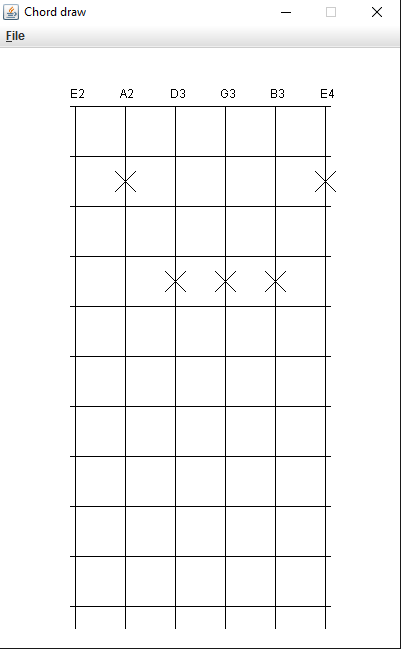
\includegraphics[width=1.0\textwidth]{../img/chords/ChordDraw}
\end{minipage}

\end{Slide}

\begin{Slide}{Modell av gitarr och ukulele}
\begin{Code}
object model {

  type Tuning = Vector[String]
  type Grip = Vector[Int]

  trait Chord {
    def name: String
    def tuning: Tuning
    def grip: Grip
  }
  
  case class Guitar(name: String, grip: Grip) extends Chord {
    val tuning = Vector("E2", "A2", "D3", "G3", "B3", "E4")
  }
  
  case class Ukulele(name: String, grip: Grip) extends Chord {
    val tuning = Vector("G4", "C4", "E4", "A4")
  }

}
\end{Code}
\end{Slide}

\begin{Slide}{En gemensam bastyp för olika ackord}\SlideFontSmall
\vspace{-0.5em}\begin{center}
\newcommand{\TextBox}[1]{\raisebox{0pt}[1em][0.5em]{#1}}
\tikzstyle{umlclass}=[rectangle, draw=black,  thick, anchor=north, text width=3cm, rectangle split, rectangle split parts = 3]
\begin{tikzpicture}[inner sep=0.5em]
\node [umlclass, rectangle split parts = 2, xshift=0cm, text width=5cm] (BaseType)  {
            \textit{\textbf{\centerline{\TextBox{\code{Chord}}}}}
            \nodepart[]{second}
            \TextBox{\code{def name: String}}\vspace{-0.25em}\newline
            \TextBox{\code{def tuning: Vector[String]}}\vspace{-0.25em}\newline
            \TextBox{\code{def grip: Vector[Int]}}\vspace{-0.25em}\newline

        };
        
\node [umlclass, rectangle split parts = 1]  at (2.5cm,-3.7cm) (SubType1) {
            \textbf{\centerline{\TextBox{\code{Guitar}}}}
            %\nodepart[]{second} \TextBox{~}
        };  
                
\node [umlclass, rectangle split parts = 1] at (-2.5cm,-3.7cm) (SubType2)  {
            \textbf{\centerline{\TextBox{\code{Ukulele}}}}
            %\nodepart[]{second} \TextBox{talk(): void}
        };        
\draw[umlarrow] (SubType1.north) -- ++(0,0.5) -| (BaseType.south);    
\draw[umlarrow] (SubType2.north) -- ++(0,0.5) -| (BaseType.south);            
\end{tikzpicture}
\end{center}
\pause\vspace{-0.7em}
\begin{REPL}
scala> import model._

scala> val uc = Ukulele("C", Vector(0, 0, 0, 3))
uc: model.Ukulele = Ukulele(C,Vector(0, 0, 0, 3))

scala> val ge = Guitar("E", Vector(0, 2, 2, 1, 0, 0))
ge: model.Guitar = Guitar(E,Vector(0, 2, 2, 1, 0, 0))
\end{REPL}
\end{Slide}


\begin{Slide}{Grupparbete}\SlideFontSmall
\begin{itemize}
\item Förslag på arbetssätt:
\begin{itemize}\SlideFontSmall
\item Träffas nu på rasten och boka nästa gruppmöte
\item Förberedelser inför första gruppmötet: individuella studier av labbinstruktioner och koden som är given i workspace \\
\href{https://github.com/lunduniversity/introprog/tree/master/workspace/w08_chords_team/src}{.../workspace/w08\_chords\_team/src} \\
OBS! numrering av labbarna enl. ''gamla'' veckor
\item Träffas gärna i ett studierum med whiteboard
\item På mötet: gå igenom uppgift och given kod så att alla fattar vad det går ut på; bestäm omfattning och ansvarsuppdelning
\item När ni träffas, skissa upp den kod som just du håller på med på whiteboard och få feedback och ge feedback till andra
\item På varje gruppmöte, bestäm tid för nästa möte och vad var och en ska försöka hinna tills dess
\end{itemize}


\item Ni får \Emph{lov att ändra på omfattningen} efter antalet gruppmedlemmar, ambition och förmåga: diskutera detta med handledare på resurstid

\item \Alert{Minimikrav}: att med textkommando kunna skapa/spara/ladda gitarr- och ukulele-ackord och att ni tränar på matchning

\end{itemize}
\end{Slide}


\Subsection{Matchning}

\begin{Slide}{Vad är matchning?}
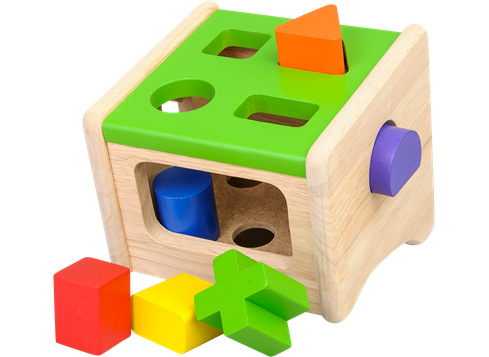
\includegraphics[width=0.8\textwidth]{../img/plocklada.png}
\end{Slide}


\begin{Slide}{Vad är matchning?}
Matchning gör man då man vill jämföra ett värde mot andra värden och hitta överensstämmelse \Eng{match}.

\pause

\vspace{1em}Detta kan man t.ex. göra med nästlade if-else-satser/uttryck:

\begin{Code}
val g = scala.io.StdIn.readLine("grönsak:")
val smak = 
  if (g == "gurka") "gott!"
  else if (g == "tomat") "jättegott!"
  else if (g == "broccoli") "ganska gott..."
  else "inte gott :("

println(g + " är " + smak)
\end{Code}
\end{Slide}




\begin{Slide}{Javas switch-sats}\SlideFontSmall
De flesta C-liknande språk (men inte Scala) har en \jcode{switch}-sats som man kan använda istället för (vissa) nästlade if-else-satser: 
\javainputlisting[basicstyle=\ttfamily\SlideFontSize{5.5}{6.8}\selectfont]{../compendium/examples/match/Switch.java}

\vspace{-0.5em}Funkar bara för primitiva typer och några till (t.ex. String).
\end{Slide}




\begin{Slide}{Javas switch-sats utan break}\SlideFontSmall
Saknad \jcode{break}-sats ''faller igenom'' till efterföljande gren: 

\javainputlisting[basicstyle=\ttfamily\SlideFontSize{6}{7}\selectfont]{../compendium/examples/match/SwitchNoBreak.java}
En glömd \jcode{break} kan ge svårhittad bugg... 
\end{Slide}

\begin{Slide}{Javas switch-sats med glömd break}\SlideFontSmall

\vspace{-0.5em}\javainputlisting[basicstyle=\ttfamily\SlideFontSize{5.5}{6.8}\selectfont]{../compendium/examples/match/SwitchForgotBreak.java}

\vspace{-0.7em}\pause
\begin{REPL}
$ java SwitchForgotBreak 
Skriv grönsak:
gurka
gott!
gott!
\end{REPL}

\end{Slide}


\begin{Slide}{Scalas \texttt{match}-uttryck}\SlideFontSmall
Scala har ingen \code{switch}-sats men erbjuder i stället ett \code{match}-\Emph{uttryck} som är kraftfullare och ger ett värde.

\begin{Code}
val g = scala.io.StdIn.readLine("grönsak:")
val smak = g match {
  case "gurka" => "gott!"
  case "tomat" => "jättegott!"
  case "broccoli" => "ganska gott..."
  case _ => "mindre gott..."
}
println(g + " är " + smak)
\end{Code}
Och den ''faller inte igenom'' som Javas \code{switch}-sats! 
\begin{itemize}
\pause\item Varje \code{case}-gren testas var för sig i tur och ordning uppifrån och ned.
\pause\item Det som står mellan \code{case} och \code{=>} kallas ett \Emph{mönster} \Eng{pattern}
\pause\item Sista default-grenen ovan kallas \Emph{wildcard-mönster}: \code{case _ => } 
\pause\item Ovan är exempel på matchning mot \Emph{konstant-mönster}, \\ i detta fallet tre stycken strängkonstantmönster.
\pause\item Det finns många andra sätt att skriva mönster.
\end{itemize}
\end{Slide}



\begin{Slide}{Matchning med gard}
Man kan stoppa in en s.k \Emph{gard} \Eng{guard} innan pilen \code{=>} för att villkora matchningen: (notera \code{if}, parenteser behövs ej)
\begin{Code}
val g = scala.io.StdIn.readLine("grönsak:")
def f = g match {
  case "gurka" if math.random > 0.5 => "gott ibland!"
  case "tomat" => "jättegott!"
  case "broccoli" => "ganska gott..."
  case _ => "mindre gott..."
}
\end{Code}
\code{case}-grenen med gard ger bara en lyckad matchning \\ om uttrycket efter \code{if} är sant; annars provas nästa gren, etc.
\end{Slide}

\begin{Slide}{Matchning med variabelmönster}\SlideFontSmall
Om det finns ett namn efter \code{case} som börjar med liten begynnelsebokstav, blir detta namn en variabel som automatiskt binds till uttrycket före \code{match}:

\begin{Code}
val g = scala.io.StdIn.readLine("grönsak:")
def f = g match {
  case "gurka" if math.random > 0.5 => "gott ibland!"
  case "tomat" => "jättegott!"
  case "broccoli" => "ganska gott..."
  case other => "smakar bakvänt: " + other.reverse
}
\end{Code}

Ett enkelt variabelmönster, så som \\ \code{case other => ...} \\ i exemplet ovan, matchar \Emph{allt}! \\\code{other} får alltså värdet av \code{g} om \code{g} \Alert{inte} är \code{"gurka"}, \code{"tomat"}, \code{"broccoli"}.  

\end{Slide}





\begin{Slide}{Matchning med typade mönster}\SlideFontSmall
Med en typannotering efter en variabel får man ett \Emph{typat mönster} \Eng{typed pattern}. Om matchningen lyckas blir värdet \Alert{omvandlat} till den specifika typen och binds till variabeln.
\begin{Code}
def f = if (math.random < 0.5) 42 + math.random else "gurka" + math.random
def g = f match {
  case x: Double => x.round.toInt
  case s: String => s.length
}
\end{Code}
Vad har funktionen \code{f} för returtyp? \\ \pause
Matchning mot specifika typer enl. ovan används i idiomatisk Scala hellre än \code{isInstanceOf} men man kan göra motsvarande ovan med if-uttryck:
\begin{Code}
def g2 = {
  val x = f
  if (x.isInstanceOf[Double]) x.asInstanceOf[Double].round.toInt
  else if (x.isInstanceOf[String]) x.asInstanceOf[String].length
}.asInstanceOf[Int]
\end{Code}
\end{Slide}


\begin{Slide}{Konstruktormönster med case-klasser}\SlideFontSmall
En basklass med gemensamma delar och två subtyper:
\begin{Code}
trait Grönsak {
  def vikt: Int
  def ärRutten: Boolean
}
case class Gurka(vikt: Int, ärRutten: Boolean) extends Grönsak
case class Tomat(vikt: Int, ärRutten: Boolean) extends Grönsak
\end{Code}
\pause
Tack vare case-klasserna kan man använda \Emph{konstruktormönster} \Eng{constructor pattern} för att kolla vad som finns \Alert{inuti} en instans:
\begin{Code}
def testa(g: Grönsak): String = g match {
  case Gurka(v, false) => "gott, väger " + v
  case Gurka(_, true)  => "inte gott"
  case Tomat(v, r)     => (if (r) "inte " else "") + "gott, väger " + v 
  case _ => "okänd grönsak: " + g
}
\end{Code}

Konstruktormönster ''\Emph{plockar isär}'' det som matchas och binder variabler till de attribut som finns i case-klassens konstruktor.
\end{Slide}


\begin{Slide}{Plocka isär samlingar med djupa mönster}
Man kan plocka isär innehållet i en samling så här:
\begin{Code}
def visa(xs: Vector[Grönsak]): String = xs match {
  case Vector()               => "tom grönsaksvektor"
  case Vector(Gurka(v, true)) => "en rutten gurka som väger " + v
  case Vector(g)              => "exakt en grönsak: " + g
  case Vector(g1, g2)         => s"exakt två grönsaker: $g1, $g2"
  case g +: gs                => s"först en $g och sedan svansen: $gs" 
}
\end{Code}
Övning: prova ovan i REPL. Vad händer om du byter ordning på andra och tredje mönstret ovan?
\end{Slide}

\begin{Slide}{Mönstermatchning och case-objekt}
En bastyp och specifika singelobjekt av gemensam typ:
\begin{Code}
trait Färg
case object Spader  extends Färg
case object Hjärter extends Färg
case object Ruter   extends Färg
case object Klöver  extends Färg

def parallellFärg(f: Färg): Färg = f match {
  case Spader  => Klöver
  case Klöver  => Spader
  case Hjärter => Ruter
}
\end{Code}
Vilken case-gren har vi glömt? Kan kompilatorn hjälpa oss?
\pause
\begin{REPL}
scala> parallellFärg(Ruter)
scala.MatchError: Ruter (of class Ruter$)
  at .parallellFärg(<console>:18)

\end{REPL}
Runtime exception \code{:(} ~~och en bugg som kan vara svårhittad...
\end{Slide}

\begin{Slide}{Mönstermatchning och förseglade typer}
Med nyckelordet \code{sealed} får vi en kompileringsvarning \code{:)}
\begin{Code}
sealed trait Färg
case object Spader  extends Färg
case object Hjärter extends Färg
case object Ruter   extends Färg
case object Klöver  extends Färg

def parallellFärg(f: Färg): Färg = f match {
  case Spader  => Klöver
  case Klöver  => Spader
  case Hjärter => Ruter
}
\end{Code}
\begin{REPL}
// Exiting paste mode, now interpreting.

<console>:23: warning: match may not be exhaustive.
It would fail on the following input: Ruter
       def parallellFärg(f: Färg): Färg = f match {
\end{REPL}
\end{Slide}

\begin{Slide}{Stora/små begynnelsebokstäver vid matchning}
Fallgrop: att försöka matcha på värdet av en variabel som börjar med liten bokstav.
\begin{REPL}
scala> val livetsMening = 42

scala> def ärLivetsMeningBuggig(svar: Int) = svar match {
         case livetsMening => true    // lokalt namn som matchar allt!
         case _ => false
       }

scala> ärLivetsMeningBuggig(43)
res0: Boolean = true

scala> val LivetsMening = 42   // stor begynnelsebokstav

scala> def ärLivetsMening(svar: Int) = svar match {
         case LivetsMening => true    // funkar fint!
         case _ => false
       }

scala> ärLivetsMening(43)
res1: Boolean = false
\end{REPL}
\end{Slide}


\begin{Slide}{Stora/små begynnelsebokstäver vid matchning}
Ett sätt att komma runt problemet med liten begynnelsebokstav: \\
\Emph{backticks} to the rescue!
\begin{REPL}
scala> val livetsMening = 42

scala> def ärLivetsMeningBackTicks(svar: Int) = svar match {
         case `livetsMening` => true    // nu funkar det!
         case _ => false
       }

scala> ärLivetsMeningBackTicks(43)
res2: Boolean = false
\end{REPL}
\end{Slide}


\begin{Slide}{Mönster på andra ställen än i \texttt{match}}\SlideFontSmall
Mönster i \Emph{deklarationer}:
\vspace{-0.25em}\begin{REPL}
scala> case class Point(x: Int, y: Int)

scala> val p = Point(0, 1)

scala> val Point(x, y) = p          // konstruktormönster med case-klass
x: ???
y: ???

scala> val (x, y, z) = (0, 1, 2)    // konstruktormönster med tupel
x: ???
y: ???
z: ???

\end{REPL}
Mönster i \Emph{for-satser}:
\vspace{-0.25em}\begin{REPL}
scala> val xs = for ((x, y) <- Vector((1,2), (3,4))) yield x
xs: ???
\end{REPL}

\end{Slide}

\begin{Slide}{Mönster på andra ställen än i \texttt{match}}\SlideFontSmall
Mönster i \Emph{deklarationer}:
\vspace{-0.25em}\begin{REPL}
scala> case class Point(x: Int, y: Int)

scala> val p = Point(0, 1)

scala> val Point(x, y) = p          // konstruktormönster med case-klass
x: Int = 0
y: Int = 1

scala> val (x, y, z) = (0, 1, 2)    // konstruktormönster med tupel
x: Int = 0
y: Int = 1
z: Int = 2

\end{REPL}
Mönster i \Emph{for-satser}:
\vspace{-0.25em}\begin{REPL}
scala> val xs = for ((x, y) <- Vector((1,2), (3,4))) yield x
xs: scala.collection.immutable.Vector[Int] = Vector(1, 3)
\end{REPL}
\end{Slide}

\begin{Slide}{Fördjupning om mönster}
Avancerade saker för den intresserade (ingår ej): 
\begin{itemize}
\item binda variabler till mönsterdelar med \code{@}
\item partiella funktioner
\item att skapa extraherare med \code{unapply} och \code{unapplySeq}
\end{itemize}
Fördjupning:
\begin{itemize}
\item Läs mer om mönster här:  \href{http://www.artima.com/pins1ed/case-classes-and-pattern-matching.html}{\SlideFontTiny www.artima.com/pins1ed/case-classes-and-pattern-matching.html}

\item För djupare förståelse av hur \code{case} fungerar, läs speciellt om \Emph{partiella funktioner} här: \href{http://www.artima.com/pins1ed/case-classes-and-pattern-matching.html\#15.7}{\SlideFontTiny www.artima.com/pins1ed/case-classes-and-pattern-matching.html\#15.7}

\item Läs om extractors här: \href{http://www.artima.com/pins1ed/extractors.html}{\SlideFontTiny www.artima.com/pins1ed/extractors.html}

\end{itemize} 
\end{Slide}


\begin{Slide}{Fördjupning: metoden \texttt{unapply}}\SlideFontSmall
När du deklarerar en case-klass kommer kompilatorn att \Alert{automatiskt generera en metod} med namnet \Emph{\texttt{unapply}} som kan plocka isär instansen.
\begin{REPL}
scala> case class Gurka(vikt: Int, ärRutten: Boolean)

scala> Gurka.unapply // tryck TAB två gånger för att se metodhuvudet
 case def unapply(x$0: Gurka): Option[(Int, Boolean)]
 
scala> val g = Gurka(100, false)

scala> Gurka.unapply(g)
res0: Option[(Int, Boolean)] = Some((100,false))
\end{REPL}
Vi ska snart se hur \code{Option} kan hantera värden som \Emph{eventuellt} \Alert{saknas}. \\
\pause

{\SlideFontTiny\vspace{1em}\emph{Fördjupning:} Ett anrop av metoden \code{unapply} genereras av kompilatorn vid matchning och det är det som gör att case-klasser kan användas i konstruktormönster. Man kan skapa en egna s.k. extraktorer \Eng{extractors} som funkar i matchningar (se övn. 22).}
\end{Slide}







%!TEX encoding = UTF-8 Unicode
%!TEX root = ../lect-w10.tex

%%%

\Subsection{Option}


\begin{Slide}{Hur hantera saknade värden?}\SlideFontSmall
Olika sätt att hantera saknade värden:
\begin{itemize}
\item Hitta på ett specialvärde: exempel -1 för icke nedtryckt sträng
\item \code{null} om \code{AnyRef}/\code{Object} (vanligt i Java, mkt ovanligt i Scala) 
\item Använd en samling och låt tom samling representera saknat värde: \\
\code{val grip = Vector(Vector(2), Vector(7), Vector(), Vector(3))}

\item \code{Option[T]} gemensam bastyp för: \\
  \code{None} som representerar \Alert{saknat värde}, och \\ \code{Some[T]} som representerar att \Emph{värde finns}
\end{itemize}
\end{Slide}

\begin{Slide}{En gemensam bastyp för ett värde som kanske saknas}\SlideFontSmall
\vspace{-0.0em}\begin{center}
\newcommand{\TextBox}[1]{\raisebox{0pt}[1em][0.5em]{#1}}
\tikzstyle{umlclass}=[rectangle, draw=black,  thick, anchor=north, text width=3cm, rectangle split, rectangle split parts = 3]
\begin{tikzpicture}[inner sep=0.5em]
\node [umlclass, rectangle split parts = 2, xshift=0cm, text width=3.5cm] (BaseType)  {
            \textit{\textbf{\centerline{\TextBox{\code{Option[A]}}}}}
            \nodepart[]{second}
            \TextBox{\code{def get: A}}\newline
            \TextBox{\code{def isEmpty: Boolean}}

        };
        
\node [umlclass, rectangle split parts = 1]  at (-2.5cm,-3.0cm) (SubType1) {
            \textbf{\centerline{\TextBox{\code{Some[A]}}}}
            % \nodepart[]{second} \TextBox{\code{val x: A}}
        };  
                
\node [umlclass, rectangle split parts = 1] at (2.5cm,-3.0cm) (SubType2)  {
            \textbf{\centerline{\TextBox{\code{None}}}}
        };        
\draw[umlarrow] (SubType1.north) -- ++(0,0.5) -| (BaseType.south);    
\draw[umlarrow] (SubType2.north) -- ++(0,0.5) -| (BaseType.south);            
\end{tikzpicture}
\end{center}
\pause
\vspace{-0.5em}\begin{REPL}
scala> var x: Option[Int] = Some(42)

scala> x.isEmpty
res0: Boolean = false

scala> x = None

scala> x.isEmpty
res1: Boolean = true
\end{REPL}
\end{Slide}


\begin{Slide}{Option för hantering av ev. saknade värden}\SlideFontSmall
Alla vill inte berätta för Facebook vad de har för kön. \\ Förbättra Facebooks kod med ett litet Scala-program:
\begin{Code}
trait Gender
case object Male   extends Gender
case object Female extends Gender

case class Person(name: String, gender: Option[Gender])
\end{Code}
\pause
\begin{REPL}
scala> val p1 = Person("Björn",  Some(Male))
scala> val p2 = Person("Sandra", Some(Female))
scala> val p3 = Person("Andro",  None)
scala> val g2 = p2.gender
scala> def show(g: Option[Gender]): String = g match {
         case Some(x) => x.toString
         case None    => "unknown"
       }
scala> show(g2)
scala> show(p3.gender)
scala> val ps = Vector(p1,p2,p3)
scala> ps.map(_.gender).map(show)
\end{REPL}
\end{Slide}

\begin{Slide}{Några smidiga metoder på \code{Option}}\SlideFontSmall
Metoden \code{getOrElse} gör att man ofta kan undvika matchning.
\begin{Code}
var opt: Option[Int] = None

val x = opt.getOrElse(42)      // get the value or give a default if missing
\end{Code}

Flera av de vanliga samlingsmetoderna funkar, t.ex. \code{foreach} och \code{map}.
\begin{Code}
opt.foreach{x => println(x)}    // only done if value exists

opt.map{x => x + 1}             // only done if value exists

opt = Some(42)                  // change opt to now have some value

opt.foreach{x => println(x)}    // done as value now exists

opt.map{x => x + 1}             // done as value now exists

\end{Code}
\end{Slide}


\begin{Slide}{Några samlingsmetoder som ger en \code{Option}}
\begin{REPL}
scala> val (xs, ys) = (Vector(1,2,3), Vector())

scala> xs.headOption
res0: ???

scala> ys.headOption
res1: ???

scala> xs.find(_ > 1)
res2: ???

scala> xs.find(_ > 5)
res3: ???

scala> val huvudstad = Map("Sverige" -> "Sthlm", "Skåne" -> "Malmö")

scala> huvudstad.get("Skåne")
res4: ???

scala> huvudstad.get("Danmark")
res5: ???
\end{REPL}
\end{Slide}

\begin{Slide}{Några samlingsmetoder som ger en \code{Option}}
\begin{REPL}
scala> val (xs, ys) = (Vector(1,2,3), Vector())

scala> xs.headOption
res0: Option[Int] = Some(1)

scala> ys.headOption
res1: Option[Nothing] = None

scala> xs.find(_ > 1)
res2: Option[Int] = Some(2)

scala> xs.find(_ > 5)
res3: Option[Int] = None

scala> val huvudstad = Map("Sverige" -> "Sthlm", "Skåne" -> "Malmö")

scala> huvudstad.get("Skåne")
res4: Option[String] = Some(Malmö)

scala> huvudstad.get("Danmark")
res5: Option[String] = None
\end{REPL}
\end{Slide}





%!TEX encoding = UTF-8 Unicode
%!TEX root = ../lect-w10.tex

%%%



\Subsection{Undantag}
\begin{Slide}{Vad är ett undantag \Eng{exception}?}
Undantag representerar ett fel eller ett onormalt tillstånd som upptäcks under exekvering och som  behöver hanteras på särskilt sätt vid sidan av det normala exekveringsflödet. 

\vspace{1em}\href{https://sv.wikipedia.org/wiki/Undantagshantering}{sv.wikipedia.org/wiki/Undantagshantering}


\vspace{1em} Exempel på undantag:

\pause

\begin{itemize}
\item Indexering utanför vektorns indexgränser.

\item Läsning bortom filens slut.

\item Försök att öppna en fil som inte finns.

\item Minnet är slut.

\item Division med noll.

\item \code{"hej".toInt} resulterar i \\\code{java.lang.NumberFormatException}

\end{itemize}

\end{Slide}

\begin{Slide}{''Kasta'' dina egna undantag med \texttt{throw}}\SlideFontSmall
Man kan själv generera ett undantag med \code{throw}, vilket kallas att \Emph{kasta} ett undantag som (om det inte \Emph{fångas}), gör att exekveringen \Alert{avbryts}.


\begin{REPL}
scala> def pang = throw new Exception("PANG!")
pang: Nothing

scala> pang
java.lang.Exception: PANG!
  at .pang(<console>:11)
  ...
  
\end{REPL}
\pause
Olika sätt att hantera undantag: 
\begin{itemize}
\item Scala: Man kan använda ett \code{try ... catch}-uttryck och ge ett \Emph{värde} i händelse av undantag.
\item Java: Man kan använda en \code{try ... catch}-sats och \Alert{göra något} i händelse av undantag.
 
\item Scala: Man kan \Emph{kapsla in} ett undantag med \Emph{\texttt{scala.util.Try}} och förhindra att exekveringen avbryts. (Finns ej i Java; att föredra i Scala.)
\end{itemize}
\end{Slide}


\Subsection{\texttt{scala.util.Try}}

\begin{Slide}{En gemensam bastyp för något som kan misslyckas}\SlideFontSmall
\begin{Code}
import scala.util.{Try, Success, Failure}
\end{Code}

\vspace{-0.5em}\begin{center}
\newcommand{\TextBox}[1]{\raisebox{0pt}[1em][0.5em]{#1}}
\tikzstyle{umlclass}=[rectangle, draw=black,  thick, anchor=north, text width=3.0cm, rectangle split, rectangle split parts = 3]
\begin{tikzpicture}[inner sep=0.5em]
\node [umlclass, rectangle split parts = 2, xshift=0cm, text width=3.8cm] (BaseType)  {
            \textit{\textbf{\centerline{\TextBox{\code{Try[T]}}}}}
            \nodepart[]{second}
            \TextBox{\code{def get: T}}\newline
            \TextBox{\code{def isFailure: Boolean}}\newline
            \TextBox{\code{def isSuccess: Boolean}}
        };
        
\node [umlclass, rectangle split parts = 2, text width=2.2cm]  at (-2.5cm,-3.7cm) (SubType1) {
            \textbf{\centerline{\TextBox{\code{Success[T]}}}}
            \nodepart[]{second} \TextBox{\code{val value: T}}
        };  
                
\node [umlclass, rectangle split parts = 2, text width=4.2cm] at (2.5cm,-3.7cm) (SubType2)  {
            \textbf{\centerline{\TextBox{\code{Failure[T]}}}}
            \nodepart[]{second} \TextBox{\code{val exception: Throwable}}
        };        
\draw[umlarrow] (SubType1.north) -- ++(0,0.5) -| (BaseType.south);    
\draw[umlarrow] (SubType2.north) -- ++(0,0.5) -| (BaseType.south);            
\end{tikzpicture}
\end{center}
\end{Slide}

\begin{Slide}{Hantera undantag med \texttt{Try}}
\vspace{-0.5em}\begin{REPL}
scala> def pang = throw new Exception("PANG!")

scala> def kanskePang = if (math.random < 0.5) 42 else pang

scala> import scala.util.{Try, Success, Failure}

scala> def försök = Try { kanskePang }

scala> val xs = Vector.fill(15){försök}

scala> val trettonde = xs(13) match {
         case Success(value) => value
         case Failure(e) => println(e); -1
       }

scala> (xs(13).isSuccess, xs(13).isFailure)

scala> försök.foreach(println)

scala> försök.map(_ + 1)

scala> for (Success(x) <- xs) yield x
\end{REPL}
\end{Slide}

\begin{Slide}{Fördjupning: \texttt{try}-\texttt{catch}-uttryck}\SlideFontSmall
Man kan fånga undantag med ett \code{try ... catch}-uttryck:
\begin{Code}
def carola = try {
  if (math.random > 0.5) throw new Exception("stormvind")
  42
} catch { 
  case e: Exception =>
    println("Fångad av en " + e.getMessage)
    -1
}  
\end{Code}
\pause
\begin{REPL}
scala> Vector.fill(5)(carola)
Fångad av en stormvind
Fångad av en stormvind
Fångad av en stormvind
res0: scala.collection.immutable.Vector[Int] = Vector(-1, 42, 42, -1, -1)
\end{REPL}
\pause
\emph{Fördjupning:} \\ Gör övning 9-10 som visar hur man fångar undantag i Scala och Java. \\Mer om undantag i fortsättningskursen.
\end{Slide}







%!TEX encoding = UTF-8 Unicode
%!TEX root = ../lect-w10.tex

%%%

\Subsection{\texttt{equals}}
\begin{Slide}{Fördjupning: Implementera \texttt{equals} med \texttt{match}}
Det visar sig att \Emph{innehållslikhet} är \Alert{förvånansvärt komplicerat} att implementera, speciellt  i samband med arv.
\begin{itemize}
\item Det enklare fallet: Gör övningsuppgift \code{patterns:14} och implementera \code{equals} för innehållslikhet utan arv. \\ En bra träning på att använda \code{match}!

\item Svårare: Gör fördjupningsövning \code{matching:21--22} om du vill se hur en \emph{komplett} \code{equals} ska se ut som funkar i alla lägen.

\end{itemize}

Det ingår inte på tentan att själv kunna implementera en generellt fungerande \code{equals}. Men du ska förstå skillnaden mellan referenslikhet och innehållslikhet. Mer om \code{equals} i fortsättningkursen, men en liten inblick i problemet nu...
\end{Slide}

\begin{Slide}{Fördjupning: \texttt{equals} som fungerar för finala klasser}
Recept för implementation av \code{equals} som fungerar för typer som \Alert{inte} har några subtyper:
\begin{Code}
final class Gurka(val vikt: Int, ärÄtbar: Boolean) {
  override def equals(other: Any): Boolean = other match {
    case that: Gurka => vikt == that.vikt && ärÄtbar == that.ärÄtbar
    case _ => false
  }
  override def hashCode: Int = (vikt, ärÄtbar).## // ger bra hashcode
}
\end{Code}
\begin{itemize}\SlideFontSmall
  \item
  Du \Alert{måste} alltid överskugga \code{hashCode} också om du överskuggar \code{equals} annars funkar inte gurksamlingar (lång story ...)
  \item
  Notera typen \code{Any} -- detta följer hur man valde att göra i Java (tyvärr?).
  \pause
  \item
  Ett \Alert{typsäkrare} innehållslikhetstest som \Emph{garanterat} bara jämför en gurka med en gurka och inget annat:
  \begin{Code}
    def ===(other: Gurka): Boolean =
      vikt == other.vikt && ärÄtbar == other.ärÄtbar
  \end{Code}
\end{itemize}
\end{Slide}


\begin{Slide}{Fördjupning: Recept i 8 steg för arvssäker \code{equals}}\SlideFontTiny
%fungerar även för klasser som inte är \code{final}:
\setlength{\leftmargini}{0pt}
\begin{enumerate}\SlideFontTiny
\item Inför denna metod: \code{ def canEqual(other: Any): Boolean}\\Observera att typen på parametern ska vara \code{Any}. Om subklass behövs \code{override}.

\item Metoden \code{canEqual} ska ge \code{true} om \code{other} är av samma typ som \code{this}, t.ex.: \code{override def canEqual(other: Any): Boolean = other.isInstanceOf[Gurka]}

\item Inför metoden \code{equals} och var noga med att parametern har typen \code{Any}: \\ \code{override def equals(other: Any): Boolean}

\item Implementera metoden \code{equals} med ett match-uttryck som börjar så här:
\code|other match { ... } |

\item Match-uttrycket ska ha två grenar. Den första grenen ska ha ett typat mönster för den klass som ska jämföras, t.ex.: \\ \code{  case that: Gurka =>}

\item Om du implementerar \code{equals} i den klass som inför \code{canEqual}, börja med: \\ \code{(that canEqual this) &&} \\
och skapa därefter en fortsättning som baseras på innehållet i klassen, t.ex.: \code{this.vikt == that.vikt && this.längd == that.längd} \\
Om du överskuggar equals vill du nog börja med
 \code{super.equals(that) && }

\item Den andra grenen i matchningen ska vara:
\code{case _ => false}

\item Överskugga \code{hashCode}, t.ex. med tupel av attributvärden och metoden \code{##}: \\
\code{override def hashCode: Int  = (vikt, längd).## }

\end{enumerate}
\url{http://www.artima.com/pins1ed/object-equality.html}

\end{Slide}


%!TEX encoding = UTF-8 Unicode
%!TEX root = ../exercises.tex

\ifPreSolution



\Exercise{\ExeWeekTEN}\label{exe:W10}

\begin{Goals}
\item Kunna skapa och använda \code{match}-uttryck med konstanta värden, garder och mönstermatchning med case-klasser.
\item Kunna skapa och använda case-objekt för matchningar på uppräknade värden.
\item Kunna hantera saknade värden med hjälp av typen \code{Option} och mönstermatchning på \code{Some} och \code{None}.
\item Kunna fånga undantag med \code{scala.util.Try}.
\item Känna till \code{try}, \code{catch} och \code{throw}.
\item Känna till \jcode{switch}-satser i Java.
\item Känna till nyckelordet \code{sealed} och förstå nyttan med förseglade typer.
\item Känna till relationen mellan \code{hashCode} och \code{equals}.
\item Kunna skapa partiella funktioner med case-uttryck.
%\item Känna till betydelsen av små och stora begynnelsebokstäver i case-grenar i en matchning, samt förstå hur namn binds till värden in en case-gren.
%\item Kunna använda \code{flatMap} tillsammans med \code{Option} och \code{Try}.
%\item Känna till skillnaderna mellan \code{try}-\code{catch} i Scala och java.
%\item Känna till hur metoden \code{unapply} används vid mönstermatchning.
%\item Kunna implementera \code{equals} med hjälp av en \code{match}-sats, som fungerar för finala klasser utan arv.
%\item Känna till \code{null}.
\end{Goals}

\begin{Preparations}
\item \StudyTheory{10}
\end{Preparations}

\BasicTasks %%%%%%%%%%%%%%%%

\else



\ExerciseSolution{\ExeWeekTEN}

\BasicTasks %%%%%%%%%%%

\fi





\WHAT{Hur fungerar en \jcode{switch}-sats i Java (och flera andra språk)?}

\QUESTBEGIN

\Task \label{task:switch} \what~   Det händer ofta att man vill testa om ett värde är ett av många olika alternativ. Då kan man använda en sekvens av många \code{if}-\code{else}, ett för varje alternativ. Men det finns ett annat sätt i Java och många andra språk: man kan använda \jcode{switch} som kollar flera alternativ i en och samma sats, se t.ex. \href{https://en.wikipedia.org/wiki/Switch_statement}{en.wikipedia.org/wiki/Switch\_statement}.

\Subtask Skriv in nedan kod i en kodeditor. Spara med namnet \texttt{Switch.java} och kompilera filen med kommandot \texttt{javac Switch.java}. Kör den med \texttt{java Switch} och ange din favoritgrönsak som argument till programmet. Vad händer? Förklara hur \jcode{switch}-satsen fungerar.

\javainputlisting[numbers=left,basicstyle=\ttfamily\fontsize{9}{11}\selectfont]{examples/Switch.java}

\Subtask \label{subtask:break} Vad händer om du tar bort \jcode{break}-satsen på rad 16?




\SOLUTION


\TaskSolved \what


\SubtaskSolved  Beroende på första bokstaven i din favoritgrönsak får du olika svar såsom \textit{gurka är gott!} vid första bokstaven $g$.\\
Javas \jcode{switch}-sats testar den första bokstaven på favoritgrönsaken genom att stegvis jämföra den med \jcode{case}-uttrycken. Om första bokstaven \jcode{firstChar} matchar bokstaven efter ett \jcode{case} körs koden efter kolonet till \jcode{switch}-satsens slut eller tills ett \jcode{break} avbryter \jcode{switch}-satsen.\\
Matchar inte \jcode{firstChar} något \jcode{case} så finns även \jcode{default}, som körs oavsett vilken första bokstaven är, ett generellt fall.

\SubtaskSolved  Om \jcode{case 't'} körs kommer både  \textit{tomat är gott!} och \textit{broccoli är gott!} skrivas ut, man säger att koden $"$faller igenom$"$. Utan \jcode{break}-satsen i Java körs koden i efterkommande \jcode{case} tills ett \jcode{break} avbryter exekveringen eller \jcode{switch}-satsen tar slut.



\QUESTEND






\WHAT{Matcha på konstanta värden.}

\QUESTBEGIN

\Task \label{task:vegomatch} \what~   I Scala finns ingen \jcode{switch}-sats. I stället har Scala ett \code{match}-uttryck som är mer kraftfullt. Dock saknar Scala nyckelordet \jcode{break} och Scalas \code{match}-uttryck kan inte ''falla igenom'' som skedde i uppgift \ref{task:switch}\ref{subtask:break}.

\Subtask \label{subtask:vegomatch} Skriv nedan program med en kodeditor och spara i filen \texttt{Match.scala}. Kompilera med \texttt{scalac Match.scala}. Kör med \texttt{scala Match} och ge som argument din favoritgrönsak. Vad händer? Förklara hur ett \code{match}-uttryck fungerar.

\scalainputlisting[numbers=left,basicstyle=\ttfamily\fontsize{11}{12}\selectfont]{examples/Match.scala}

\Subtask Vad blir det för felmeddelande om du tar bort case-grenen för defaultvärden och indata väljs så att inga case-grenar matchar? Är det ett exekveringsfel eller ett kompileringsfel?


\Subtask Beskriv några skillnader i syntax och semantik mellan Javas flervalssats \jcode{switch} och Scalas flervalsuttryck \code{match}.




\SOLUTION


\TaskSolved \what


\SubtaskSolved  Svaret blir identiskt mot föregående uppgiften i Java.\\
Scalas \code{match}-uttryck fungerar väldigt likt Javas \jcode{switch}. Den jämför stegvis värdet med varje \code{case} för att sedan returnera ett värde tillhörande motsvarande \code{case}.

\SubtaskSolved  \begin{REPL}
scala.MatchError (of class java.lang.Character)
\end{REPL}
Exekveringsfel, uppstår av en viss input under körningen.

\SubtaskSolved  Scalas \code{match} ersätter kolonet (:) i \jcode{switch} med Scalas högerpil (=>).\\
\code{match} returnerar ett värde till skillnad från \jcode{switch} som inte returnerar något.\\
\code{match} kan inte $"$falla igenom$"$ så ett \jcode{break} efter varje \jcode{case} är inte nödvändigt.\\
Till skillnad från \jcode{switch}-satsen kastar \code{match} ett \code{MatchError} om ingen matchning skulle ske.



\QUESTEND






\WHAT{Gard i case-grenar.}

\QUESTBEGIN

\Task  \what~  Med hjälp en gard \Eng{guard} i en case-gren kan man begränsa med ett villkor om grenen ska väljas.

Utgå från koden i uppgift \ref{task:vegomatch}\ref{subtask:vegomatch} och byt ut case-grenen för \code{'g'}-matchning till nedan variant med en gard med nyckelordet \code{if} (notera att det inte behövs parenteser runt villkoret):
\begin{Code}
    case 'g' if math.random > 0.5 => "gurka är gott ibland..."
\end{Code}
Kompilera om och kör programmet upprepade gånger med olika indata tills alla grenar i \code{match}-uttrycket har exekverats. Förklara vad som händer.

\SOLUTION


\TaskSolved \what

Garden som införts vid \code{case 'g'} slumpar fram ett tal mellan 0 och 1 och om talet inte är större än $0.5$ så blir det ingen matchning med \code{case 'g'} och programmet testar vidare tills default-caset.\\
Gardens krav måste uppfyllas för att det ska matcha som vanligt.



\QUESTEND






\WHAT{Mönstermatcha på attributen i case-klasser.}

\QUESTBEGIN

\Task \label{task:match-caseclass} \what~   Scalas \code{match}-uttryck är extra kraftfulla om de används tillsammans med \code{case}-klasser: då kan attribut extraheras automatiskt och bindas till lokala variabler direkt i case-grenen som nedan exempel visar (notera att \code{v} och \code{rutten} inte behöver deklareras explicit). Detta kallas för \textbf{mönstermatchning}.

\Subtask \label{subtask:autobinding-match} Vad skrivs ut nedan? Varför? Prova att byta namn på \code{v} och \code{rutten}.
\begin{REPL}
scala> case class Gurka(vikt: Int, ärRutten: Boolean)
scala> val g = Gurka(100, true)
scala> g match { case Gurka(v,rutten) => println("G" + v + rutten) }
\end{REPL}

\Subtask Skriv sedan nedan i REPL och tryck TAB två gånger efter punkten. Vad har \code{unapply}-metoden för resultattyp?
\begin{REPL}
scala> Gurka.unapply   // Tryck TAB två gånger
\end{REPL}
\begin{Background}
Case-klasser får av kompilatorn automatiskt ett kompanjonsobjekt \Eng{companion object}, i detta fallet \code{object Gurka}. Det objektet får av kompilatorn automatiskt en \code{unapply}-metod. Det är \code{unapply} som anropas ''under huven'' när case-klassernas attribut extraheras vid mönstermatchning, men detta sker alltså automatiskt och man behöver inte explicit nyttja \code{unapply} om man inte själv vill implementera s.k. extraherare \Eng{extractors}; om du är nyfiken på detta, se fördjupningsuppgift \ref{task:extractor}.
\end{Background}

\Subtask Anropa \code{unapply}-metoden enligt nedan. Vad blir resultatet?
\begin{REPL}
scala> Gurka.unapply(g)
\end{REPL}
Vi ska i senare uppgifter undersöka hur typerna \code{Option} och \code{Some} fungerar och hur man kan ha nytta av dessa i andra sammanhang.

% \Subtask Spara programmet nedan i filen \texttt{vegomatch.scala} och kompilera och kör med \code{scala vegomatch.Main 1000} i terminalen. Förklara hur predikatet \code{ärÄtvärd} fungerar.
% \scalainputlisting[numbers=left,basicstyle=\ttfamily\fontsize{11}{12}\selectfont]{examples/vegomatch.scala}
%

\SOLUTION


\TaskSolved \what


\SubtaskSolved  G100true. Vid byte av plats: Gtrue100.\\
\code{match} testar om kompanjonsobjektet \code{Gurka} är av typen \code{Gurka} med två parametervärden. De angivna parametrarna tilldelas namn, \code{vikt} får namnet \code{v} och \code{ärRutten} namnet \code{rutten} och skrivs sedan ut. Byts namnen dessa ges skrivs de ut i den omvända ordningen.

\SubtaskSolved  \code{Option[(Int, Boolean)]}

\SubtaskSolved  \code{Some((100, true))}, en \code{Option} med en tupel av parametrarna från g.

% \SubtaskSolved  \code{ärÄtvärd} testar om \code{Grönsak g} är av typen \code{Gurka(v, rutten)} eller \code{Tomat}. Dessa har sedan garder.\\ \code{Gurka} måste ha \code{vikt} över 100 och \code{ärRutten} vara \code{false} för att \code{case Gurka} ska returnera \code{true}.\\
% \code{Tomat} måste ha \code{vikt} över 50 och \code{ärRutten} vara \code{false} för att \code{case Tomat} ska returnera \code{true}.\\
% Matchas inte \code{Grönsak g} med någon av dessa returneras default-värdet \code{false}.



\QUESTEND







\WHAT{Matcha på case-objekt och nyttan med \code{sealed}.}

\QUESTBEGIN

\Task  \what~  Skapa nedan kod i en editor, och klistra in i REPL med kommandot \code{:pa}. Notera nyckelordet \code{sealed} som används för att försegla en typ. En \textbf{förseglad typ} måste ha alla sina subtyper i en och samma kodfil.
\begin{Code}
sealed trait Färg
object Färg {
  val values = Vector(Spader, Hjärter, Ruter, Klöver)
}
case object Spader  extends Färg
case object Hjärter extends Färg
case object Ruter   extends Färg
case object Klöver  extends Färg
\end{Code}

\Subtask Skapa en funktion \code{def parafärg(f: Färg): Färg} i en editor, som med hjälp av ett match-uttryck returnerar parallellfärgen till en färg. Parallellfärgen till \code{Hjärter} är \code{Ruter} och vice versa, medan parallellfärgen till \code{Klöver} är \code{Spader} och vice versa. Klistra in funktionen i REPL.
\begin{REPL}
scala> parafärg(Spader)
scala> val xs = Vector.fill(5)(Färg.values((math.random * 4).toInt))
scala> xs.map(parafärg)
\end{REPL}

\Subtask Vi ska nu undersöka vad som händer om man glömmer en av case-grenarna i matchningen i \code{parafärg}. ''Glöm'' alltså avsiktligt en av case-grenarna och klistra in den nya \code{parafärg} med den ofullständiga matchningen. Hur lyder varningen? Kommer varningen vid körtid eller vid kompilering?

\Subtask Anropa \code{parafärg} med den ''glömda'' färgen. Hur lyder felmeddelandet? Är det ett kompileringsfel eller ett körtidsfel?

\Subtask Förklara vad nyckelordet \code{sealed} innebär och vilken nytta man kan ha av att \textbf{försegla} en supertyp.


\SOLUTION


\TaskSolved \what


\SubtaskSolved
\begin{Code}
def parafärg(f: Färg): Färg = f match {
  case Spader  => Klöver
  case Hjärter => Ruter
  case Ruter   => Hjärter
  case Klöver  => Spader
}
\end{Code}

\SubtaskSolved
\begin{REPL}
<console>:17: warning: match may not be exhaustive.
It would fail on the following input: Ruter
\end{REPL}
Varningen kommer redan vid kompilering.

\SubtaskSolved
\begin{REPL}
scala.MatchError: Ruter (of class Ruter)
  at .parafärg(<console>:17)
\end{REPL}
Detta är ett körtidsfel.

\SubtaskSolved  Om en klass är \code{sealed} innebär det att om ett element ska matchas och är en subtyp av denna klass så ger Scala varning redan vid kompilering om det finns en risk för ett \code{MatchError}, alltså om \code{match}-uttrycket inte är uttömmande och det finns fall som inte täcks av ett \code{case}.\\
En förseglad supertyp innebär att programmeraren redan vid kompileringstid får en varning om ett fall inte täcks och i sånt fall vilket av undertyperna, liksom annan hjälp av kompilatorn. Detta kräver dock att alla subtyperna delar samma fil som den förseglade klassen.



\QUESTEND






\WHAT{Betydelsen av små och stora begynnelsebokstäver vid matchning.}

\QUESTBEGIN

\Task  \what~  För att åstadkomma att namn kan bindas till variabler vid matchning utan att de behöver deklareras i förväg (som vi såg i uppgift \ref{task:match-caseclass}\ref{subtask:autobinding-match}) så har identifierare med liten begynnelsebokstav fått speciell betydelse: den tolkas av kompilatorn som att du vill att en variabel  binds till ett värde vid matchningen. En identifierare med stor begynnelsebokstav tolkas däremot som ett konstant värde (t.ex. ett case-objekt eller ett case-klass-mönster).

\Subtask \emph{En case-gren som fångar allt}. En case-gren med en identifierare med liten begynnelsebokstav som saknar gard kommer att matcha allt. Prova nedan i REPL, men försök lista ut i förväg vad som kommer att hända. Vad händer?
\begin{REPL}
scala> val x = "urka"
scala> x match {
         case str if str.startsWith("g") => println("kanske gurka")
         case vadsomhelst => println("ej gurka: " + vadsomhelst)
       }
scala> val g = "gurka"
scala> g match {
         case str if str.startsWith("g") => println("kanske gurka")
         case vadsomhelst => println("ej gurka: " + vadsomhelst)
       }
\end{REPL}

\Subtask \emph{Fallgrop med små begynnelsbokstäver.} Innan du provar nedan i REPL, försök gissa vad som kommer att hända. Vad händer? Hur lyder varningarna och vad innebär de?
\begin{REPL}
scala> val any: Any = "varken tomat eller gurka"
scala> case object Gurka
scala> case object tomat
scala> any match {
         case Gurka => println("gurka")
         case tomat => println("tomat")
         case _ => println("allt annat")
       }
\end{REPL}

\Subtask \emph{Använd backticks för att tvinga fram match på konstant värde.} Det finns en utväg om man inte vill att kompilatorn ska skapa en ny lokal variabel: använd specialtecknet \emph{backtick}, som skrivs \`{} och kräver speciella tangentbordstryck.\footnote{Fråga någon om du inte hittar hur man gör backtick \`{} på ditt tangentbord.}  Gör om föregående uppgift men omgärda nu identifieraren \code{tomat} i tomat-case-grenen med backticks, så här: \code{  case `tomat` => ...}



\SOLUTION


\TaskSolved \what


\SubtaskSolved  Både \code{str} och \code{vadsomhelst} matchar med inputen, oavsett vad denna är på grund av att de har en liten begynnelsebokstav.\\
 \code{str} har dock en gard att strängen måste börja med $g$ vilket gör så endast \code{val g = "gurka"} matchar med denna. \code{val x = "urka"} plockas dock upp av \code{vadsomhelst} som är utan gard.

\SubtaskSolved
\begin{REPL}
<console>:16: warning: patterns after a variable pattern cannot match (SLS 8.1
.1)
\end{REPL}
och
\begin{REPL}
<console>:17: warning: unreachable code due to variable patter 'tomat' on line
16
\end{REPL}
Trots att en klass \code{tomat} existerar så tolkar Scalas \code{match} den som en \code{case}-gren som fångar allt på grund av en liten begynnelsebokstav. Detta gör så alla objekt som inte är av typen \code{Gurka} kommer ge utskriften \textit{tomat} och att sista caset inte kan nås.

\SubtaskSolved
\begin{Code}
case `tomat` => println("tomat")
\end{Code}



\QUESTEND






\WHAT{Använda \code{Option} och matcha på värden som kanske saknas.}

\QUESTBEGIN

\Task  \what~  Man behöver ofta skriva kod för att hantera värden som eventuellt saknas, t.ex. saknade telefonnummer i en persondatabas. Denna situation är så pass vanlig att många språk har speciellt stöd för saknande värden.

I Java\footnote{Scala har också \code{null} men det behövs bara vid samverkan med Java-kod.} används värdet \code{null} för att indikera att en referens saknar värde. Man får då komma ihåg att testa om värdet saknas varje gång sådana värden ska behandlas, t.ex. med \code+if (ref != null) { ...} else { ... }+. Ett annat vanligt trick är att låta \code{-1} indikera saknade positiva heltal, till exempel saknade index, som får behandlas med \code+if (i != -1) { ...} else { ... }+.

I Scala finns en speciell typ \code{Option} som möjliggör smidig och typsäker hantering av saknade värden. Om ett kanske saknat värde packas in i en \code{Option} \Eng{wrapped in an Option}, finns det i en speciell slags samling som bara kan innehålla \emph{inget} eller \emph{något} värde, och alltså har antingen storleken \code{0} eller \code{1}.

\Subtask Förklara vad som händer nedan.
\begin{REPL}
scala> var kanske: Option[Int] = None
scala> kanske.size
scala> kanske = Some(42)
scala> kanske.size
scala> kanske.isEmpty
scala> kanske.isDefined
scala> def ökaOmFinns(opt: Option[Int]): Option[Int] = opt match {
         case Some(i) => Some(i + 1)
         case None    => None
       }
scala> val annanKanske = ökaOmFinns(kanske)
scala> def öka(i: Int) = i + 1
scala> val merKanske = kanske.map(öka)
\end{REPL}

\Subtask Mönstermatchingen ovan är minst lika knölig som en \code{if}-sats, men tack vare att en \code{Option} är en slags (liten) samling finns det smidigare sätt. Förklara vad som händer nedan.
\begin{REPL}
val meningen = Some(42)
val ejMeningen = Option.empty[Int]
meningen.map(_ + 1)
ejMeningen.map(_ + 1)
ejMeningen.map(_ + 1).orElse(Some("saknas")).foreach(println)
meningen.map(_ + 1).orElse(Some("saknas")).foreach(println)
\end{REPL}

\Subtask \emph{Samlingsmetoder som ger en \code{Option}.} Förklara för varje rad nedan vad som händer. En av raderna ger ett felmeddelande; vilken rad och vilket felmeddelande?
\begin{REPL}
val xs = (42 to 84 by 5).toVector
val e = Vector.empty[Int]
xs.headOption
xs.headOption.get
xs.headOption.getOrElse(0)
xs.headOption.orElse(Some(0))
e.headOption
e.headOption.get
e.headOption.getOrElse(0)
e.headOption.orElse(Some(0))
Vector(xs, e, e, e)
Vector(xs, e, e, e).map(_.lastOption)
Vector(xs, e, e, e).map(_.lastOption).flatten
xs.lift(0)
xs.lift(1000)
e.lift(1000).getOrElse(0)
xs.find(_ > 50)
xs.find(_ < 42)
e.find(_ > 42).foreach(_ => println("HITTAT!"))
\end{REPL}

\Subtask Vilka är fördelerna med \code{Option} jämfört med \code{null} eller \code{-1} om man i sin kod glömmer hantera saknade värden?

\SOLUTION


\TaskSolved \what


\SubtaskSolved  \begin{enumerate}
\item \code{var kanske} blir en \code{Option} som håller \code{Int} men är utan något värde, kallas då \code{None}.
\item Eftersom \code{var kanske} är utan värde är storleken av den 0.
\item \code{var kanske} tilldelas värdet 42 som förvaras i en \code{Some} som visar att värde finns.
\item Eftersom \code{var kanske} nu innehåller ett värde är storleken 1.
\item Eftersom \code{var kanske} innehåller ett värde är den inte tom.
\item Eftersom \code{var kanske} innehåller ett värde är den definierad.
\item \code{def ökaOmFinns} matchar en \code{Option[Int]} med dess olika fall.\\
Finns ett värde, alltså \code{opt: Option[Int]} är en \code{Some}, så returneras en \code{Some} med ursprungliga värdet plus 1.\\
Finns inget värde, alltså \code{opt: Option[Int]} är en \code{None}, så returneras en \code{None}.
\item -
\item -
\item -
\item \code{def ökaOmFinns} appliceras på \code{kanske} och returnerar en \code{Some} med värdet hos \code{kanske} plus 1, alltså 43.
\item \code{def öka} tar emot värdet av en \code{Int} och returnerar värdet av denna plus 1.
\item \code{map} applicerar \code{def öka} till det enda elementen i \code{kanske}, 42. Denna funktion returnerar en \code{Some} med värdet 43 som tilldelas \code{merKanske}.
\end{enumerate}

\SubtaskSolved  \begin{enumerate}
\item \code{val meningen} blir en \code{Some} med värdet 42.
\item \code{val ejMeningen} blir en \code{Option[Int]} utan något värde, en \code{None}.
\item \code{map(_ + 1)} appliceras på \code{meningen} och ökar det existerande värdet med 1 till 43.
\item \code{map(_ + 1)} appliceras på \code{ejMening} men eftersom inget värde existerar fortsätter denna vara \code{None}.
\item \code{map(_ + 1)} appliceras ännu en gång på \code{ejMening} men denna gång inkluderas metoden \code{orElse}. Om ett värde inte existerar hos en \code{Option}, alltså är av typen \code{None}, så utförs koden i \code{orElse}-metoden som i detta fall skriver ut \textit{saknas} för värdet som saknas.
\item Samma anrop från föregående rad utförs denna gång på \code{meningen} och eftersom ett värde finns utförs endast första biten som ökar detta värde med 1.
\end{enumerate}
Denna metod kan användas i stället för \code{match}-versionen i föregående exempel i och med dennas simplare form. En \code{Option} innehåller ju antingen ett värde eller inte så ett längre \code{match}-uttryck är inte nödvändigt.

\SubtaskSolved \begin{enumerate}
\item En vektor \code{xs} skapas med var femte tal från 42 till 82.
\item En tom \code{Int}-vektor \code{e} skapas.
\item \code{headOption} tar ut första värdet av vektorn \code{xs} och returnerar den sparad i en \code{Option}, \code{Some(42)}.
\item Första värdet i vektorn \code{xs} sparas i en \code{Option} och hämtas sedan av \code{get}-metoden, 42.
\item Som i föregående rad men denna gång används \code{getOrElse} som om den \code{Option} som returneras saknar ett värde, alltså är av typen \code{None}, returnerar 0 istället.\\
 Eftersom \code{xs} har minst ett värde så är den \code{Option} som returneras inte \code{None} och ger samma värde som i föregående, 42.
\item Som föregående rad fast istället för att returnera 0 om värde saknas så returneras en \code{Option[Int]} med 0 som värde.
\item \code{headOption} försöker ta ut första värdet av vektorn \code{e} men eftersom denna saknar värden returneras en \code{None}.
\item \begin{REPL}
java.util.NoSuchElementException: None.get
\end{REPL}
Liksom föregående rad returnerar \code{headOption} på den tomma vektorn \code{e} en \code{None}. När  \code{get}-metoden försöker hämta ett värde från en \code{None} som saknar värde ger detta upphov till ett körtidsfel.
\item Liksom i föregående returneras \code{None}  av \code{headOption} men eftersom \code{getOrElse}-metoden används på denna \code{None} returneras 0 istället.
\item Liksom föregående används \code{getOrElse}-metoden på den \code{None} som returneras. Denna gång returneras dock en \code{Option[Int]} som håller värdet 0.
\item En vektor innehållandes elementen \code{xs}-vektorn och 3 \code{e}-vektorer skapas.
\item \code{map} använder metoden \code{lastOption} på varje delvektor från vektorn på föregående rad. Detta sammanställer de sista elementen från varje delvektor i en ny vektor. Eftersom vektor \code{e} är tom returneras \code{None} som element från denna.
\item Samma sker som i föregående rad men \code{flatten}-metoden appliceras på slutgiltiga vektorn som rensar vektorn på \code{None} och lämnar endast faktiska värden.
\item \code{lift}-metoden hämtar det eventuella värdet på plats 0  i \code{xs} och returnerar den i en \code{Option} som blir \code{Some(42)}.
\item \code{lift}-metoden försöker hämta elementet på plats 1000 i \code{xs}, eftersom detta inte existerar returneras \code{None}.
\item  Samma sker som i föregående fast applicerat på vektorn \code{e}. Sedan appliceras \code{getOrElse(0)} som, eftersom \code{lift}-metoden returnerar \code{None}, i sin tur returnerar 0.
\item \code{find}-metoden anropas på \code{xs}-vektorn. Den letar upp första talet över 50 och returnerar detta värde i en \code{Option[Int]}, alltså \code{Some(52)}.
\item \code{find}-metoden anropas på \code{xs}-vektorn. Den letar upp första värdet under 42 men eftersom inget värde existerar under 42 i \code{xs} returneras \code{None} istället.
\item \code{find}-metoden anropas på \code{e}-vektorn och skriver ut \textit{HITTAT!} om ett element under 42 hittas. Eftersom \code{e}-vektorn är tom returneras \code{None} vilket \code{foreach} inte räknar som element och därav inte utförs på.
\end{enumerate}

\SubtaskSolved  Användning av -1 som returvärde vid fel eller avsaknad på värde kan ge upphov till körtidsfel som är svåra att upptäcka. \jcode{null} kan i sin tur orsaka kraschar om det skulle bli fel under körningen. \code{Option} har inte samma problem som dessa, används ett \code{getOrElse}-uttryck eller dylikt så kraschar inte heller programmet.\\
Dessutom behöver inte en funktion som returnerar en \code{Option} samma dokumentation av returvärdena. Istället för att skriva kommentarer till koden på vilka värden som kan returneras och vad dessa betyder så syns det direkt i koden.\\
Slutgiltligen är \code{Option} mer typsäkert än \code{null}. När du returnerar en \code{Option} så specificeras typen av det värde som den kommer innehålla, om den innehåller något, vilket underlättar att förstå och begränsar vad den kan returnera.



\QUESTEND






\WHAT{Kasta undantag.}

\QUESTBEGIN

\Task  \what~  Om man vill signalera att ett fel eller en onormal situtation uppstått så kan man \textbf{kasta} \Eng{throw} ett \textbf{undantag} \Eng{exception}. Då avbryts programmet direkt med ett felmeddelande, om man inte väljer att \textbf{fånga} \Eng{catch} undantaget.

\Subtask Vad händer nedan?
\begin{REPL}
scala> throw new Exception("PANG!")
scala> java.lang.   // Tryck TAB efter punkten
scala> throw new IllegalArgumentException("fel fel fel")
scala> val carola = try {
         throw new Exception("stormvind!")
         42
       } catch { case e: Throwable => println("Fångad av en " + e); -1 }
\end{REPL}
\Subtask Nämn ett par undantag som finns i paketet \code{java.lang} som du kan gissa vad de innebär och i vilka situationer de kastas.

\Subtask Vilken typ har variabeln \code{carola} ovan? Vad hade typen blivit om catch-grenen hade returnerat en sträng i stället?

\SOLUTION


\TaskSolved \what


\SubtaskSolved  \begin{enumerate}
\item Ett \code{Exception} kastas med felmeddelandet \textit{PANG!}.
\item Flera olika typer av \code{Exception} visas.
\item En typ av \code{Exception}, \code{IllegalArgumentException}, kastas med felmeddelandet \textit{fel fel fel}.
\item Ett stycke kod testas med \code{try}. Ett \code{Exception} med felmeddelandet \textit{stormvind!} kastas som fångas av \code{catch}-uttrycket. Den matchar felmeddelandet såsom ett \code{match}-uttryck och det godtyckliga fallet \code{e} skriver ut det \code{Exception} som fångats och returnerar -1.
\end{enumerate}

\SubtaskSolved  Exempelvis: \\
\code{OutOfMemoryError}, om programmet får slut på minne.\\
\code{IndexOutOfBoundsException}, om en vektorposition som är större än vad som finns hos vektorn försöker nås.\\
\code{NullPointerException}, om en metod eller dylikt försöker användas hos ett objekt som inte finns och därav är en nullreferens.

\SubtaskSolved  Eftersom värdet som skulle vara av typen \code{Int} känner \code{try}-funktionen igen returtypen hos \code{case e} och \code{carola} blir av typen \code{Int}. Skulle \code{catch}-grenen returnera en sträng istället vet programmet inte vilken typ denna är av och \code{carola} blir av typen \code{Any}.



\QUESTEND






\WHAT{Fånga undantantag i Java med en \jcode{try}-\jcode{catch}-sats.}

\QUESTBEGIN

\Task \label{task:javatry} \what~   Det finns som vi såg i förra uppgiften inbyggt stöd i JVM för att hantera när program avbryts på oväntade sätt, t.ex. på grund av division med noll eller ej förväntade indata från användaren. Skriv in nedan Java-program i en editor och spara i en fil med namnet \texttt{TryCatch.java} och kompilera med \texttt{javac TryCatch.java} i terminalen.

\javainputlisting[numbers=left,basicstyle=\ttfamily\fontsize{11}{12}\selectfont]{examples/TryCatch.java}

\Subtask Förklara vad som händer när du kör programmet med olika indata:
\begin{REPL}
> java TryCatch 42
> java TryCatch 0
> java TryCatch safe 42
> java TryCatch safe 0
> java TryCatch
\end{REPL}

\Subtask Vad händer om du ''glömmer bort'' raden 15 och därmed missar att initialisera input? Hur lyder felmeddelandet? Är det ett körtidsfel eller kompileringsfel?

\Subtask Beskriv några skillnader och likheter i syntax och semantik mellan \code{try}-\code{catch} i Java respektive Scala.



\SOLUTION


\TaskSolved \what


\SubtaskSolved  \begin{enumerate}
\item Eftersom första argumentet inte är strängen \textit{safe} görs en oskyddad division av 42 med 42 där slutsvaret 1 visas.
\item Eftersom första argumentet inte är strängen \textit{safe} görs en oskyddad division av 42 med 0 som ger \code{ArithmeticException} eftersom ett tal inte kan delas med noll.
\item Eftersom första argumentet är strängen \textit{safe} görs en skyddad division av 42 med 42 där slutsvaret 1 visas.
\item Eftersom första argumentet är strängen \textit{safe} görs en skyddad division av 42 med 0. Denna gång fångas \code{ArithmeticException} av \code{try-catch}-satsen vilket ersätter den gamla division med en säker division med 1 där slutsvaret 42 visas.
\item Eftersom inga argument givits kastas ett \code{ArrayIndexOutOfBoundsException} när programmet försöker anropa \code{equals} metoden hos en sträng som inte finns. Detta kunde också kontrollerats av en \code{try-catch}-sats.
\end{enumerate}

\SubtaskSolved  \begin{REPL}
TryCatch.java:16: error: variable input might not have been initialized
\end{REPL}
Ett kompileringsfel uppstår på grund av risken att \code{input} inte blivit definierad vid division.

\SubtaskSolved  Den mest markanta skillnaden mellan språken är att Scala varken kräver att ett undantag fångas av en \code{catch} eller att ett undantag behöver deklareras innan det kastas med en \code{@throws}. Dessutom saknar \code{catch}-metoden hos Java de \code{match}-egenskaper Scala har. Inte heller returnerar \code{catch} hos Java något värde vilket gör det nödvändigt att definiera variabler för detta innan. I övrigt är semantiken och syntaxen väldigt lika mellan båda språken. De använder samma struktur och samma ord, dessutom har de en hel del \code{Exception} gemensamt.



\QUESTEND






\WHAT{Fånga undantantag i Scala med \code{scala.util.Try}.}

\QUESTBEGIN

\Task  \what~  I paketet \code{scala.util} finns typen \code{Try} med stort T som är som en slags samling som kan innehålla antingen ett ''lyckat'' eller ''misslyckat'' värde. Om beräkningen av värdet lyckades och inga undantag kastas blir värdet inkapslat i en \code{Success}, annars blir undantaget inkapslat i en \code{Failure}. Man kan extrahera värdet, respektive undantaget, med mönstermatchning, men det är oftast smidigare att använda samlingsmetoderna \code{map} och \code{foreach}, i likhet med hur \code{Option} används. Det finns även en smidig metod \code{recover} på objekt av typen \code{Try} där man kan skicka med kod som körs om det uppstår en undantagssituation.

\Subtask Förklara vad som händer nedan.
\begin{REPL}
scala> def pang = throw new Exception("PANG!")
scala> import scala.util.{Try, Success, Failure}
scala> Try{pang}
scala> Try{pang}.recover{case e: Throwable =>   "desarmerad bomb: " + e}
scala> Try{"tyst"}.recover{case e: Throwable => "desarmerad bomb: " + e}
scala> def kanskePang = if (math.random > 0.5) "tyst" else pang
scala> def kanskeOk = Try{ kanskePang}
scala> val xs = Vector.fill(100)(kanskeOk)
scala> xs(13) match {
         case Success(x) => ":)"
         case Failure(e) => ":( " + e
       }
scala> x(13).isSuccess
scala> x(13).isFailure
scala> xs.count(_.isFailure)
scala> xs.find(_.isFailure)
scala> val badOpt = xs.find(_.isFailure)
scala> val goodOpt = xs.find(_.isSuccess)
scala> badOpt
scala> badOpt.get
scala> badOpt.get.get
scala> badOpt.map(_.getOrElse("bomben desarmerad!")).get
scala> goodOpt.map(_.getOrElse("bomben desarmerad!")).get
scala> xs.map(_.getOrElse("bomben desarmerad!")).foreach(println)
scala> xs.map(_.toOption)
scala> xs.map(_.toOption).flatten
scala> xs.map(_.toOption).flatten.size
\end{REPL}


\Subtask Vad har funktionen \code{pang} för returtyp?

\Subtask Varför får funktionen \code{kanskePang} den härledda returtypen \code{String}?

\SOLUTION


\TaskSolved \what


\SubtaskSolved  \begin{enumerate}
\item \code{def pang} skapas som kastar ett \code{Exception} med felmeddelandet \textit{PANG!}.
\item Scalas verktyg \code{Try}, \code{Success} och \code{Failure} importeras.
\item \code{def pang} anropas i \code{Try} som fångar undantaget och kapslar in den i en \code{Failure}.
\item Metoden \code{recover} matchar undantaget i \code{Failure} från föregående rad med ett \code{case} och gör om föredetta \code{Failure} till \code{Success} vid matchning, liknande \code{catch}.
\item Strängen \textit{tyst} körs i föregående test men eftersom inget undantag kastas blir den inkapslad i en \code{Success} och \code{recover} behöver inte göra något. Den tar endast hand om undantag.
\item \code{def kanskePang} skapas som har lika stor chans att returnera strängen \textit{tyst} såsom anropa \code{def pang}.
\item \code{def kanskeOk} skapas som testar \code{def kanskePang} med \code{Try}.
\item En vektor \code{xs} fylls med resultaten, \code{Success} och \code{Failure}, från 100 körningar av \code{kanskeOk}.
\item Elementet på plats 13 i vektor \code{xs} matchas med något av 2 \code{case}. Om det är en \code{Success} skrivs \textit{:)} ut, om en \code{Failure} skrivs \textit{:(} plus felmeddelandet ut.
\item -
\item -
\item -
\item Metoden \code{isSuccess} testar om elementet på plats 13 i \code{xs} är en \code{Success} och returnerar \code{true} om så är fallet.
\item Metoden \code{isFailure} testar om elementet på plats 13 i \code{xs} är en \code{Failure} och returnerar \code{true} om så är fallet.
\item Metoden \code{count} räknar med hjälp av \code{isFailure} hur många av elementen i \code{xs} som är \code{Failure} och returnerar detta tal.
\item Metoden \code{find} letar upp med hjälp av \code{isFailure} ett element i \code{xs} som är \code{Failure} och returnerar denna i en \code{Option}.
\item \code{badOpt} tilldelas den första \code{Failure} som hittas i \code{xs}.
\item \code{goodOpt} tilldelas den första \code{Success} som hittas i \code{xs}.
\item Resultatet badOpt skrivs ut, \code{Option[scala.util.Try[String]] =}\\
\code{Some(Failure(java.lang.Exception: PANG!))}
\item Metoden \code{get} hämtar från \code{badOpt} den \code{Failure} som förvaras i en \code{Option}.
\item Metoden \code{get} anropas ännu en gång på resultatet från föregående rad, alltså en \code{Failure}, som hämtar undantaget från denna och som då i sin tur kastas.
\item Metoden \code{getOrElse} anropas på den \code{Failure} som finns i \code{badOpt}. Eftersom detta är en \code{Exception} utförs \code{orElse}-biten istället för att undantaget försöker hämtas. Då returneras strängen \textit{bomben desarmerad!}.
\item Metoden \code{getOrElse} anropas på den \code{Success} som finns i \code{goodOpt}. Eftersom detta är en \code{Success} med en normal sträng sparad i sig returneras denna sträng, \textit{tyst}.
\item Metoden från föregående används denna gång på alla element i \code{xs} där resultatet skrivs ut för varje.
\item Metoden \code{toOption} appliceras på alla \code{Success} och \code{Failure} i \code{xs}. De med ett exception, alltså \code{Failure}, blir en \code{None} medan de med värden i \code{Success} ger en \code{Some} med strängen \textit{tyst} i sig.
\item Metoden \code{flatten} appliceras på vektorn fylld med \code{Option} från föregående rad för att ta bort alla \code{None}-element.
\item Metoden \code{size} används på slutgiltiga listan från föregående rad för att räkna ut hur många \code{Some} som resultatet innehåller. Den har alltså beräknat antalet element i \code{xs} som var av typen \code{Success} med hjälp av \code{Option}-typen.
\end{enumerate}

\SubtaskSolved  \code{pang} har returtypen \code{Nothing}, en specialtyp inom Scala som inte är kopplad till \code{Any}, och som inte går att returnera.

\SubtaskSolved  Typen \code{Nothing} är en subtyp av varenda typ i Scalas hierarki. Detta innebär att den även är en subtyp av \code{String} vilket implicerar att \code{String} inkluderar både strängar och \code{Nothing} och därav blir returtypen.



\QUESTEND


\clearpage
\AdvancedTasks %%%%%%%%%%%%%%%%%%%



\WHAT{Använda matchning eller dynamisk bindning?}

\QUESTBEGIN

\Task  \what~ Man kan åstadkomma urskiljningen av de ätbara grönsakerna i uppgift \ref{task:match-caseclass} med dynamisk bindning i stället för \code{match}.

\Subtask Gör en ny variant av ditt program enligt nedan riktlinjer och spara den modifierade koden i filen \texttt{vegopoly.scala} och kompilera och kör.
\begin{itemize}[noitemsep]
\item Ta bort predikatet \code{ärÄtvärd} i objektet \code{Main} och inför i stället en abstrakt metod \code{def ärÄtbar: Boolean} i traiten \code{Grönsak}.
\item Inför konkreta \code{val}-medlemmar i respektive grönsak som definierar ätbarheten.
\item Ändra i huvudprogrammet i enlighet med ovan ändringar så att \code{ärÄtvärd} anropas som en metod på de skördade grönsaksobjekten när de ätvärda ska filtreras ut.
\end{itemize}

\Subtask Lägg till en ny grönsak \code{case class Broccoli} och definiera dess ätbarhet. Ändra i slump-funktionerna så att broccoli blir ovanligare än gurka.

\Subtask Jämför lösningen med \code{match} i uppgift \ref{task:match-caseclass} och lösningen ovan med polymorfism. Vilka är för- och nackdelarna med respektive lösning? Diskutera två olika situationer på ett hypotetiskt företag som utvecklar mjukvara för jordbrukssektorn: 1) att uppsättningen grönsaker inte ändras särskilt ofta medan definitionerna av ätbarhet ändras väldigt ofta och 2) att uppsättningen grönsaker ändras väldigt ofta men att ätbarhetsdefinitionerna inte ändras särskilt ofta.



\SOLUTION


\TaskSolved \what


\SubtaskSolved
\begin{Code}
package vegopoly

trait Grönsak {
	def vikt: Int
	def ärRutten: Boolean
	def ärÄtbar: Boolean
}

case class Gurka(vikt: Int, ärRutten: Boolean) extends
	Grönsak { val ärÄtbar: Boolean = (!ärRutten && vikt > 100)}
case class Tomat(vikt: Int, ärRutten: Boolean) extends
	Grönsak { val ärÄtbar: Boolean = (!ärRutten && vikt > 50)}

object Main{
	def slumpvikt: Int = (math.random*500 + 100).toInt
	def slumprutten: Boolean = math.random > 0.8
	def slumpgurka: Gurka = Gurka(slumpvikt, slumprutten)
	def slumptomat: Tomat = Tomat(slumpvikt, slumprutten)
	def slumpgrönsak: Grönsak = if (math.random > 0.2) slumpgurka
		else slumptomat

	def main(args: Array[String]): Unit = {
		val skörd = Vector.fill(args(0).toInt)(slumpgrönsak)
		val ätvärda = skörd.filter(_.ärÄtbar)
		println("Antal skördade grönsaker: " + skörd.size)
		println("Antal ätvärda grönsaker: " + ätvärda.size)
	}
}
\end{Code}

\SubtaskSolved
Följande \code{case class} läggs till:
\begin{Code}
case class Broccoli(vikt: Int, ärRutten: Boolean)
    extends Grönsak {
  val ärÄtbar: Boolean = (!ärRutten && vikt > 80)
}
\end{Code}
~\\
Därefter läggs följande till i \code{object Main} innan \code{def slumpgrönsak}:

\begin{Code}
def slumpbroccoli: Broccoli = Broccoli(slumpvikt, slumprutten)
\end{Code}
~\\
Slutligen ändras \code{def slumpgrönsak} till följande:

\begin{Code}
def slumpgrönsak: Grönsak = {    // välj t.ex. denna fördelning:
  val rnd = math.random
  if (rnd > 0.5) slumpgurka      // 50% sannolikhet för gurka
  else if (rnd > 0.2) slumptomat // 30% sannolikhet för tomat
  else slumpbroccoli             // 20% sannolikhet för broccoli
}
\end{Code}

\SubtaskSolved  Fördelarna med \code{match}-versionen, och mönstermatchning i sig, är att det är väldigt lätt att göra ändringar på hur matchningen sker. Detta innebär att det skulle vara väldigt lätt att ändra definitionen för ätbarheten. Skulle dock dessa inte ändras ofta utan snarare grönsaksutbudet så kan det polyformistiska alternativet vara att föredra. Detta eftersom det skulle implementeras och ändras lättare än mönstermatchningen vid byte av grönsaker.



\QUESTEND





\WHAT{Metoden \code{equals}.}

\QUESTBEGIN

\Task  \what~   Om man överskuggar den befintliga metoden \code{equals} så kommer metoden \code{==} att fungera annorlunda. Man kan då själv åstadkomma innehållslikhet i stället för referenslikhet. Vi börjar att studera den befintliga equals med referenslikhet.

\Subtask \label{subtask:refequals} Vad händer nedan? Om du trycker TAB \emph{två} gånger efter ett metodnamn får du se metodens signatur. Vilken signatur har metoden \code{equals}?
\begin{REPL}
scala> class Gurka(val vikt: Int, ärÄtbar: Boolean)
scala> val g1 = new Gurka(42, true)
scala> val g2 = g1
scala> val g3 = new Gurka(42, true)
scala> g1 == g2
scala> g1 == g3
scala> g1.equals  // tryck TAB två gånger
\end{REPL}

\Subtask Rita minnessituationen efter rad 4.

\Subtask \emph{Överskugga metoderna \code{equals} och \code{hashCode}.}

\begin{Background}
Det visar sig förvånande komplicerat att implementera innehållslikhet med metoden \code{equals} så att den ger bra resultat under alla speciella omständigheter. Till exempel måste man även överskugga en metod vid namn \code{hashCode} om man överskuggar \code{equals}, eftersom dessa båda används gemensamt av effektivitetsskäl för att skapa den interna lagringen av objekten i vissa samlingar. Om man missar det kan objekt bli ''osynliga'' i \code{hashCode}-baserade samlingar -- men mer om detta i senare kurser. Om objekten ingår i en öppen arvshierarki blir det också mer komplicerat; det är enklare om man har att göra med finala klasser. Dessutom krävs speciella hänsyn om klassen har en typparameter.
\end{Background}

\noindent Definera klassen nedan i REPL med överskuggade \code{equals} och \code{hashCode}; den ärver inte något och är final.

\begin{Code}
// fungerar fint om klassen är final och inte ärver något
final class Gurka(val vikt: Int, ärÄtbar: Boolean) {
  override def equals(other: Any): Boolean = other match {
    case that: Gurka => this.vikt == that.vikt
    case _ => false
  }
  override def hashCode: Int = (vikt, ärÄtbar).## //förklaras sen
}
\end{Code}
\Subtask Vad händer nu nedan, där \code{Gurka} nu har en överskuggad \code{equals} med innehållslikhet?
\begin{REPL}
scala> val g1 = new Gurka(42, true)
scala> val g2 = g1
scala> val g3 = new Gurka(42, true)
scala> g1 == g2
scala> g1 == g3
\end{REPL}
\Subtask Hur märker man ovan att den överskuggade \code{equals} medför att \code{==} nu ger innehållslikhet? Jämför med deluppgift \ref{subtask:refequals}.

I uppgift \ref{task:equals:Complex} får du prova på att följa det fullständiga receptet i 8 steg för att överskugga en \code{equals} enligt konstens alla regler. I efterföljande kurs kommer mer träning i att hantera innehållslikhet och hash-koder. I Scala får man ett objekts hash-kod med metoden \code{##}.\footnote{Om du är nyfiken på hash-koder, läs mer här:
\href{https://en.wikipedia.org/wiki/Java_hashCode()}{en.wikipedia.org/wiki/Java\_hashCode()}.}



\SOLUTION


\TaskSolved \what


\SubtaskSolved  \begin{enumerate}
\item En klass \code{Gurka} skapas med parametrarna \code{vikt} av typen \code{Int} och ärÄtbar av typen \code{Boolean}.
\item \code{g1} tilldelas en instans av \code{Gurka}-klassen med \code{vikt = 42} och \code{ärÄtbar = true}.
\item \code{g2} tilldelas samma \code{Gurka}-objekt som g1.
\item \code{g3} tilldelas en ny instans av \code{Gurka}-klassen med motsvarande parametrar som g1.
\item \code{==}(\code{equals})-metoden jämför g1 med g2 och returnerar \code{true}.
\item \code{==}(\code{equals})-metoden jämför g1 med g3 och returnerar \code{false}.
\item \code{def equals(x\$1: Any): Boolean}
\end{enumerate}
Som kan ses ovan är elementet som jämförs i \code{equals} av typen \code{Any}. Eftersom programmet inte känner till klassen så används \code{Any.equals} vid jämförelsen. Till skillnad från de primitiva datatyperna som vid jämförelse med \code{equals} jämför innehållslikhet, så jämförs referenslikheten hos klasser om inget annat är specificerat. \code{g1} och \code{g2} refererar till samma objekt medan \code{g3} pekar på ett eget sådant vilket innebär att \code{g1} och \code{g3} inte har referenslikhet.

\SubtaskSolved  \\
\vspace{1em}
\tikzstyle{mybox} = [draw=red, fill=blue!20, very thick,
    rectangle, rounded corners, inner sep=10pt, inner ysep=20pt]
\begin{tikzpicture}[
	font=\large\sffamily,
	varname/.style={node distance=0.2cm},
	varbox/.style={draw, node distance=0.2cm},
	objcloud/.style={cloud, cloud puffs=15.7, cloud ignores aspect, align=center, draw},
]

\node [varname] (g1var) {\texttt{g1}};
\node [varbox, right = of g1var] (g1ref) {\phantom{abc}};
\filldraw[black] (g1ref) circle (3pt) node[] (g1dot) {};
\node [objcloud, right = of g1ref, yshift=1.3cm, scale =0.8] (g1obj) {
	\texttt{\textbf{Gurka}} \\~\\ \texttt{vikt} \framebox{42} ~ \texttt{ärÄtvärd} \framebox{true}
};
\draw [arrow] (g1dot) -- (g1obj);

\node [varname, below = of g1var] (g2var) {\texttt{g2}};
\node [varbox, right = of g2var] (g2ref) {\phantom{abc}};
\filldraw[black] (g2ref) circle (3pt) node[] (g2dot) {};
\node [objcloud, right = of g2ref, yshift=-1.3cm, scale =0.8] (g2obj) {
	\texttt{\textbf{Gurka}} \\~\\ \texttt{vikt} \framebox{42} ~ \texttt{ärÄtvärd} \framebox{true}
};
\draw [arrow] (g2dot) -- (g1obj);
\node [varname, below = of g2var] (g3var) {\texttt{g3}};
\node [varbox, right = of g3var] (g3ref) {\phantom{abc}};
\filldraw[black] (g3ref) circle (3pt) node[] (g3dot) {};
\draw [arrow] (g3dot) -- (g2obj);

\end{tikzpicture}

\SubtaskSolved  -

\SubtaskSolved  I de första 3 raderna sker samma som i deluppgift \textit{a}. När nu dessa jämförelser görs mellan \code{Gurka}-objekten så överskuggas \code{Any.equals} av den \code{equals} som är specificerad för just \code{Gurka}. Eftersom båda objekten \code{g1} jämförs med också är av typen \code{Gurka} så matchar den med \code{case that: Gurka}. Denna i sin tur jämför vikterna hos de båda gurkorna och returnerar en \code{Boolean} huruvida de är lika eller inte, vilket de i båda fallen är.

\SubtaskSolved  I deluppgift a gav \code{g1 == g3 false} trots innehållslikhet. Efter skuggningen ger dock detta uttryck \code{true} vilket påvisar jämförelse av innehållslikhet.



\QUESTEND






\WHAT{Polynom.}

\QUESTBEGIN

\Task \label{task:polynomial} \what~   Med hjälp av koden nedan, kan man göra följande:
\begin{REPL}
scala> :pa polynomial.scala

scala> import polynomial._

scala> Const(1) * x
res0: polynomial.Term = x

scala> (x*5)^2
res1: polynomial.Prod = 25x^2

scala> Poly(x*(-5), y^4, (z^2)*3)
res2: polynomial.Poly = -5x + y^4 + 3z^2

\end{REPL}

\Subtask Förklara vad som händer ovan genom att studera koden för \code{object polynomial} nedan i filen \code{polynomial.scala}.\footnote{Koden finns även här:\\ \href{https://github.com/lunduniversity/introprog/tree/master/compendium/examples/polynomial}{github.com/lunduniversity/introprog/tree/master/compendium/examples/polynomial}}

\scalainputlisting[numbers=left,basicstyle=\ttfamily\fontsize{10}{12}\selectfont]{examples/polynomial/polynomial.scala}

\Subtask Bygg vidare på \code{object polynomial} och implementera addition mellan olika termer.


\SOLUTION


\TaskSolved \what


\SubtaskSolved \TODO

\SubtaskSolved \TODO



\QUESTEND






\WHAT{\code{Option} som en samling.}

\QUESTBEGIN

\Task  \what~Studera dokumentationen för \code{Option} här och se om du känner igen några av metoderna som också finns på samlingen \code{Vector}:\\ \href{http://www.scala-lang.org/api/current/scala/Option.html}{www.scala-lang.org/api/current/scala/Option.html}
\\Förklara hur metoden \code{contains} på en \code{Option} fungerar med hjälp av dokumentationens exempel.



\SOLUTION


\TaskSolved \what \TODO


\QUESTEND






\WHAT{Fånga undantag med \code{catch} i Java och Scala.}

\QUESTBEGIN

\Task  \what~ Gör motsvarande program i Scala som visas i uppgift \ref{task:javatry}, men utnyttja att Scalas \code{try}-\code{catch} är ett uttryck. Kompilera och kör och testa så att de ur användarens synvinkel fungerar precis på samma sätt. Notera de viktigaste skillnaderna mellan de båda programmen.


\SOLUTION


\TaskSolved \what \TODO


\QUESTEND


\AdvancedTasks %%%%%%%%%




\WHAT{Polynom, fortsättning: reducering.}

\QUESTBEGIN

\Task  \what~ Bygg vidare på \code{object polynomial} i uppgift \ref{task:polynomial} på sidan \pageref{task:polynomial} och implementera metoden \code{def reduce: Poly} i case-klassen \code{Poly} som förenklar polynom om flera \code{Prod}-termer kan adderas.

\SOLUTION


\TaskSolved \what



\QUESTEND




\WHAT{Hash-koder.}

\QUESTBEGIN

\Task  \what~ Läs om hash-koder här: \href{https://en.wikipedia.org/wiki/Java_hashCode()}{en.wikipedia.org/wiki/Java\_hashCode()} \\
Vad ger metoden \code{##} i scala.Any för resultat? Läs dokumentationen här: \\ \href{http://www.scala-lang.org/api/current/scala/Any.html}{www.scala-lang.org/api/current/scala/Any.html}

\SOLUTION


\TaskSolved \what



\QUESTEND






\WHAT{Typsäker innehållstest med metoden \code{===}.}

\QUESTBEGIN

\Task  \what~  Metoderna \code{equals} och \code{==} tillåter jämförelse med vad som helst. Ibland vill man ha en typsäker innehållsjämförelse som bara tillåter jämförelse av objekt av en mer specifik typ och ger kompileringsfel annars. Man brukar då definiera en metod \code{===} som har en parameter \code{that} som har en så specifik typ som önskas. Inför nedan abstrakta metod \code{===} i traiten \code{polynomial.Term} i uppgift \ref{task:polynomial} på sidan \pageref{task:polynomial} och överskugga den sedan i alla subklasser till Term. Testa så att du får kompileringsfel om du försöker jämföra en \code{Term} med något helt annat, t.ex. en \code{String} eller \code{Vector}.
\begin{Code}
  def ===(that: Term): Boolean
\end{Code}


\SOLUTION


\TaskSolved \what



\QUESTEND






\WHAT{Överskugga \code{equals} med innehållslikhet även för icke-finala klasser.}

\QUESTBEGIN

\Task \label{task:equals:Complex} \what~   Nedan visas delar av klassen \code{Complex} som representerar ett komplext tal med realdel och imaginärdel. I stället för att, som man ofta gör i Scala, använda en case-klass och en \code{equals}-metod som automatiskt ger innehållslikhet, ska du träna på att implementera en egen \code{equals}.
\begin{Code}
class Complex(val re: Double, val im: Double) {
  def abs: Double = math.hypot(re, im)
  override def toString = s"Complex($re, $im)"
  def canEqual(other: Any): Boolean = ???
  override def hashCode: Int  = ???
  override def equals(other: Any): Boolean = ???
}
case object Complex {
  def apply(re: Double, im: Double): Complex = new Complex(re, im)
}
\end{Code}
Följ detta \textbf{recept}\footnote{Detta recept bygger på \url{http://www.artima.com/pins1ed/object-equality.html}} i 8 steg för att överskugga \code{equals} med innehållslikhet som fungerar även för klasser som inte är \code{final}:

\begin{enumerate}[leftmargin=*]
\item Inför denna metod: \code{ def canEqual(other: Any): Boolean}\\Observera att typen på parametern ska vara \code{Any}. Om detta görs i en subklass till en klass som redan implementerat \code{canEqual}, behövs även \code{override}.

\item Metoden \code{canEqual} ska ge \code{true} om \code{other} är av samma typ som \code{this}, alltså till exempel: \\
\code{def canEqual(other: Any): Boolean = other.isInstanceOf[Complex]}

\item Inför metoden \code{equals} och var noga med att parametern har typen \code{Any}: \\ \code{override def equals(other: Any): Boolean}

\item Implementera metoden \code{equals} med ett match-uttryck som börjar så här:
\code|other match { ... } |

\item Match-uttrycket ska ha två grenar. Den första grenen ska ha ett typat mönster för den klass som ska jämföras: \\ \code{  case that: Complex =>}

\item Om du implementerar \code{equals} i den klass som inför \code{canEqual}, börja uttrycket med: \\ \code{(that canEqual this) &&} \\
och skapa därefter en fortsättning som baseras på innehållet i klassen, till exempel: \code{this.re == that.re && this.im == that.im} \\
Om du överskuggar en \textit{annan} equals än den standard-equals som finns i \code{AnyRef}, vill du förmodligen börja det logiska uttrycket med att anropa superklassens equals-metod:
 \code{super.equals(that) && } men du får fundera noga på vad likhet av underklasser egentligen ska innebära i ditt speciella fall.

\item Den andra grenen i matchningen ska vara:
\code{case _ => false}

\item Överskugga \code{hashCode}, till exempel genom att göra en tupel av innehållet i klassen och anropa metoden \code{##} på tupeln så får du i en bra hashcode: \\
\code{override def hashCode: Int  = (re, im).## }

\end{enumerate}


\SOLUTION


\TaskSolved \what



\QUESTEND






\WHAT{Överskugga equals vid arv.}

\QUESTBEGIN

\Task  \what~ Bygg vidare på exemplet nedan och överskugga equals vid arv, genom att följa receptet i uppgift \ref{task:equals:Complex}.
\begin{Code}
trait Number {
  override def equals(other: Any): Boolean = ???
}
class Complex(re: Double, im: Double) extends Number {
  override def equals(other: Any): Boolean = ???
}
class Rational(numerator: Int, denominator: Int) extends Number {
  override def equals(other: Any): Boolean = ???
}
\end{Code}


\SOLUTION


\TaskSolved \what



\QUESTEND






\WHAT{Speciella matchningar.}

\QUESTBEGIN

\Task  \what~ Läs om olika speciella matchningar här: \\
\href{http://www.artima.com/pins1ed/case-classes-and-pattern-matching.html}{www.artima.com/pins1ed/case-classes-and-pattern-matching.html}

\Subtask Prova variabelbinding med \texttt{@} i en matchning i REPL.

\Subtask Prova sekvensmönster med \texttt{\_} och \texttt{\_*} i en matching i REPL.

\SOLUTION


\TaskSolved \what



\QUESTEND






\WHAT{Extraktorer.}

\QUESTBEGIN

\Task \label{task:extractor} \what~  Läs mer om extraktorer här: \\ \href{http://www.artima.com/pins1ed/extractors.html}{www.artima.com/pins1ed/extractors.html} \\
Skapa ditt eget extraktor-objekt för http-addresser som i t.ex.: \\
\texttt{http://my.host.domain/path/to/this} \\ extraherar \texttt{my.host.domain} och \texttt{path/to/this} med metoden \code{unapply} och testa i en matchning.

%\Task \TODO \emph{flatten och flatMap med Option och Try}
%Ska detta vara ordinarie uppgift eller fördjupning???


%\Task \TODO \emph{partiella funktioner och metoderna collect och collectFirst på samlingar}
%Ska detta vara ordinarie uppgift eller fördjupning???

\SOLUTION


\TaskSolved \what --



\QUESTEND




\WHAT{Polynom, fortsättning: polynomdivision.}

\QUESTBEGIN

\Task  \what~ En rejäl utmaning: Implementera polynomdivision på lämpligt sätt genom att bygga vidare på  \code{object polynomial} i  uppgift \ref{task:polynomial} på sidan \pageref{task:polynomial}.  \\ Läs mer om polynomdivision här: \href{https://sv.wikipedia.org/wiki/Polynomdivision}{sv.wikipedia.org/wiki/Polynomdivision}

\SOLUTION


\TaskSolved \what --

\QUESTEND

%!TEX encoding = UTF-8 Unicode

%!TEX root = ../compendium2.tex

\Lab{\LabWeekTEN}

\begin{Goals}
\item Kunna använda mönstermatchning.
\item Kunna förklara hur \code{Option} användas för att hantera saknde värden.
\item Känna till att \code{scala.util.Try} kan användas för att hantera undantag.
\item Känna till att undantag kan hanteras med \code{try catch}.

\end{Goals}

\begin{Preparations}
\item Gör övning {\tt \ExeWeekTEN} i kapitel \ref{chapter:W10}.
\item Testa så att datorn du ska använda på redovisningen kan spela upp ljud med \code{javax.sound.midi} genom att köra igång \code{Main} i den givna koden.
\item Det är bra om du kan ta med hörlurar till laborationen så att du inte stör andra.
\end{Preparations}

\subsection{Bakgrund}
När man skriver program skapar man ofta modeller av en viss verklig \emph{domän}, som kan vara t.ex. försäkringskassans regelverk eller en fysiksimulering i ett datorspel. För att kunna skapa sådana modeller behöver man ofta skaffa sig  \emph{domänkunskap} genom att noga sätta sig in i vad olika koncept i domänen innebär och hur de är relaterade. Med denna kunskap kan du skapa kod som modellerar domänen, utifrån noga valda förenklingar av den komplexa verkligheten. Förmåga att kunna skapa domänmodeller utgör en viktig grund för konsten att utveckla bra programvarusystem, och du kommer lära dig mer om detta i kommande kurser.

I denna laboration ska du skapa ett program baserat på en förenklad modell av domänen \emph{musik}. Du får färdig kod som modellerar hur toner är uppbyggda, samt hur olika stränginstrument fungerar.
Med denna domänmodell ska du skapa ditt eget musikprogram som använder \emph{ackord} som är uppbyggda av flera toner som spelas tillsammans.

\subsection{Domänmodell}


\subsubsection{Tonhöjd}

En \textbf{ton} \Eng{note} som spelas på ett instrument, t.ex. ett piano eller en gitarr, har en \textbf{tonhöjd} \Eng{pitch} som är relaterad till den specifika  grundfrekvens som tonens ljud har. I vår modell av musikdomänen tillordnar vi olika distinkta tonhöjder ett unikt heltal. En tonhöjd kan då beskrivas av en \code{case class Pitch(nbr: Int)} där vi använder \code{nbr} i intervallet \code{(0 to 127)}. Heltalet \code{60} motsvarar en viss ton, som även har namnet  \code{"C5"}, och som ligger ungefär i mitten av tangentbordet på ett piano.

Inom (västerländsk) musik utgår man från 12 olika \emph{tonklasser} \Eng{pitch classes}.
Dessa tolv tonklasser är ordnade i en sekvens av så kallade \emph{halva tonsteg} och har följande \textbf{tonklassnamn}:
\begin{Code}
  val pitchClassNames: Vector[String] =
    Vector("C","C#","D","D#","E","F","F#","G","G#","A","A#","B")
\end{Code}
Efter tonklassen med namnet \code{B} återkommer tonklassen med namnet \code{C}.
Symbolen \code{#} representerar en höjning ett halvt tonsteg. Tonklassen \code{C#} uttalas \emph{siss} på svenska, och \emph{see sharp} på engelska.\footnote{Man använder även b-förtecknet $\flat$, som uttalas \emph{flat} på engelska, för sänkning av en ton ett halvt tonsteg, men för enkelhetens skull bortser vi i vår modell från detta sätt att namnge toner.}
 Notera att det är ett halvt tonsteg mellan \code{E} och \code{F}, samt mellan \code{B} och \code{C} (det finns därför varken \code{E#} eller \code{B#} i listan med tonklassnamn.\footnote{Varför det är på detta viset kan du läsa mer om på t.ex. Wikipedia, men du kan också nöja dig med att det helt enkelt är så på grund av historiska skäl.})

På ett piano motsvaras de vita tangenterna av tonklassnamen \code{C D E F G A B} och de svarta tangenterna motsvaras av tonklassnamnen \code{C# D# F# G# A#}.

En s.k. \textbf{tonklass} är ett positivt heltal i intervallet \code{0 until 12} som motsvaras av index för tonklassnamnet i \code{pitchClassNames}. En tonhöjd  \code{Pitch(nbr)} tillhör tonklassen \code{nbr % 12}.

Med hjälp av heltalsdivision med 12 får man fram tonhöjdens så kallade \textbf{oktav}, alltså \code{nbr / 12}. Ett piano har normalt toner som spänner över 7 eller 8 oktaver.
En tonhöjd \code{Pitch(nbr)} kan även namnges med en kombination av tonklassnamnet och tonens oktav, t.ex. \code{"C5"}.

Med denna domänbeskrivning kan vi skapa en mer detaljerad modell av konceptet tonhöjd med hjälp av en case-klass och tillhörande kompanjonsobjekt:

\scalainputlisting[basicstyle=\ttfamily\fontsize{10}{13}\selectfont]{../workspace/w10_music/src/main/scala/music/Pitch.scala}

\noindent Kompanjonsobjektet har två fabriksmetoder som kan skapa \code{Pitch}-objekt från en strängrepresentation av en tonhöjd.

\begin{itemize}[noitemsep]
  \item Metoden \code{fromString} omvandlar en sträng till en \code{Option[Pitch]}.

  \item Metoden \code {apply} kastar ett undantag om det inte går att omvandla en sträng till ett \code{Pitch}-objekt.
\end{itemize}

\Task\label{music:exceptions}\Pen Vilka två uttryck i \code{Try}-blocket kan ge undantag? Undersök liknande undantagsuttryck i REPL och skriv ner namnet på undantagen.


\Task Undersök klassen \code{Pitch} i REPL.

\begin{REPL}
> sbt
sbt> console
Welcome to Scala 2.12.3 (Java HotSpot(TM) 64-Bit Server VM, Java 1.8.0_144).

scala> import music._
import music._

scala> Pitch("C#5").nbr
res0: Int = 61

scala> Pitch("C") + 1
res1: music.Pitch = Pitch("C#5")
\end{REPL}


\Subtask\Pen Ge ett exempel på argument till \code{Pitch.apply} som gör att undantag kastas.

\Subtask\Pen Ge ett exempel på argument till \code{Pitch.fromString} som ger \code{None}.

\Subtask\Pen Ge ett exempel på argument till \code{Pitch.+} som gör att undantag kastas.


\Task Ändra i implementationen av \code{fromString} så att du i stället för \code{.toOption} gör en mönstermatchning med \code{match} på \code{Try}-resultaten \code{Success} och \code{Failure} i varsin case-klausul på formen \code{case Sucess(e) => } och \code{case Failure(e: ???) => ???} och returnera lämpligt värde. Ta endast hand om de två förväntade undantagstyperna som du identifierade i uppgift \ref{music:exceptions}. Gör så att alla övriga eventuella undantag kastas genom denna klausul: \code{case Failure(e) => throw e}

\Subtask Testa så att din lösning fungerar i både normalfall och vid felaktigt tönhöjdsnamn.

\Subtask\Pen Undersök vad som händer om du kommenterar bort olika case-klausuler. När ger kompilatorn varning? Varför?

\Subtask\Pen Finns det någon fördel resp. nackdel med att bara fånga vissa undantag?

\subsubsection{Ackord}

Ett ackord består av flera toner som spelas tillsammans. Man kan spela ett ackord på ett stränginstrument genom att slå an en mängd toner samtidigt eller en sekvens av toner i snabb följd. Man väljer att kalla en av tonerna i ackordet (oftast den lägsta/första tonen) för \textbf{grundton} \Eng{root}.

Ett \textbf{intervall} är en tons relativa tonhöjdsavstånd från grundtonen. Ackord har olika namn beroende på vilka intervall som ingår i ackordet. Det finns väldigt många olika ackordnamn, men här begränsar vi oss för enkelhetens skull till fyra olika typer av ackord: \footnote{Om du vill veta mer om ackordnamn läs här: \url{https://en.wikipedia.org/wiki/Chord_(music)}}
\begin{itemize}
  \item dur-ackord, betecknas t.ex. \code{"C"},
  \item moll-ackord, betecknas t.ex. \code{"Cm"}
  \item sju-ackord, betecknas t.ex. \code{"C7"}
  \item maj-sju-ackord som betecknas t.ex. \code{"Cmaj7"}.
\end{itemize}

I case-klassen \code{Chord} nedan finns en metod \code{name} som definerar vilka intervall som ingår i de olika ackordtyperna ovan, utom maj-sju-ackord. Den krångliga modulo-12-omräkningen innan matchningen gör så att intervall i olika oktaver behandlas lika, även för negativa intervall.

\scalainputlisting[basicstyle=\ttfamily\fontsize{10}{13}\selectfont]{../workspace/w10_music/src/main/scala/music/Chord.scala}

\Task

\Subtask Maj-sju-ackord har samma intervall som sju-ackord, förutom att det fjärde intervallet ska vara \code{11} halva tonsteg från grundtonen i stället för \code{10}. Lägg till en case-klausul i \code{Chord.name} så att maj-sju-ackord ges namn som slutar med ändelsen \code{"maj7"}.

\Subtask Testa din kod och kontrollera så att ackordet \code{Chord("D4","F#4","A4","C#5")} får namnet \code{"Dmaj7"}

\begin{REPL}
scala> Chord("D4","F#4","A4","C#5").name()
res2: String = "Dmaj7"
\end{REPL}

\Subtask Vilka fyra toner har ett \code{Cmaj7}-ackord med grundtonen \code{"C5"}?

\subsubsection{Stränginstrument}

Ett stränginstrument, t.ex. ett piano eller en gitarr, kännetecknas av att det kan spela ackord genom att flera strängar kan sättas i svängning så att många toner spelas tillsammans. I vår modell fångar vi denna egenskap med en trait \code{StringInstrument} som har en metod \code{toChordOpt} som ger något ackord om minst en sträng spelas.

Gitarr och ukulele är exempel på stränginstrument som har en greppbräda \Eng{fret board}. Man spelar på ett stränginstrument med greppbräda \emph{fretted instruments} genom att trycka strängar mot greppbrädan med en hand, samtidigt som man knäpper på strängarna med den andra handen. Olika instanser av dessa  instrument kan skilja sig åt vad gäller antalet strängar och hur dessa strängar är stämda. En normal gitarr har 6 strängar, medan en normal ukulele bara har 4 strängar. Dessa egenskaper modelleras i koden nedan.

Varje sträng har en stämskruv med vilken kan man ändra strängens spänning,  strängens s.k. \textbf{stämning} \Eng{tuning}.  Om man knäpper på alla lösa strängarna på en gitarr med standardstämning spelas tonerna E3, A3, D4, G4, B4, E5, räknat från den tjockaste till den tunnaste strängen.

\scalainputlisting[basicstyle=\ttfamily\fontsize{10}{12.9}\selectfont]{../workspace/w10_music/src/main/scala/music/instruments.scala}

Om man trycker på greppbrädans olika positioner får man olika toner, beroende på vilken position man trycker på. Positionerna på greppbrädan räknas från ett och uppåt. Position \code{0} motsvarar lös sträng. En negativ position, tex. \code{-1}, anger att en sträng inte spelas; många gitarrackord spelas genom att bara en delmängd av strängarna slås an.

Ett exempel på ett gitarrackord visas i figur \ref{music:fig:guitar-chord}. Detta motsvarar ackordet \code{Guitar(3,3,2,0,1,0)}, där tonen G spelas på den tjockaste strängen.

\Task\Pen Studera modellen av stränginstrument ovan och använd REPL för att svara på dessa frågor:

\Subtask Vad är namnet på detta pianoackord om vi väljer att lägsta tonen i ackordet är grundton: \code{Piano(Set(60, 64, 67, 70))}

\Subtask Vad heter tonerna som ingår i ackordet \code{Guitar(3,3,2,0,1,0)}.

\Subtask Vad heter detta ackord om vi väljer ett A som grundton: \code{ Ukulele(0,2,1,2)}


\begin{figure}
  \centering
  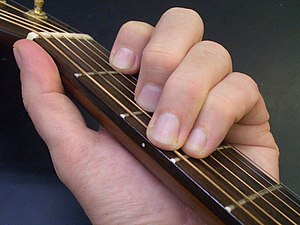
\includegraphics{../img/chords/guitar-C-major-chord.jpg}
  \caption{Ett C-dur-ackord på en gitarr med tonen G i basen.}
  \label{music:fig:guitar-chord}
\end{figure}


\subsubsection{Elektroniska instrument}

Ett elektroniskt instrument syntetiserar ljud med hjälp av analog och/eller digital elektronik, och kallas därför \textbf{synthesizer}, ofta förkortat \emph{synt} \Eng{synth}.

I JDK ingår ett api för att styra syntar. De flesta moderna datorer har ljudkort med inbyggd synt som följer den så kallade MIDI-standarden. Java-paketet \code{javax.sound.midi} innehåller klasser som kan få ett sådant ljudkort att spela musik med hjälp av MIDI.

MIDI-standarden baseras på en modell av ett pianotangentbord där olika toner kan vara ''på'' eller ''av'' beroende på om en tangent är nedtryckt eller ej. Dessa toners höjd är modellerade på samma sätt som i vår klass \code{Pitch}, där alltså tonhöjden \code{60} motsvarar tonen \code{"C5"}, etc. En tangent kan tryckas ner olika hårt, vilket representeras av ett heltalsvärde i \code{Range(0,128)} kallat \code{velocity}. Ett högt värde ger en stark ton, medan ett litet värde motsvarar en svag (tyst) ton.

En synt som följer MIDI-standarden kan spela upp ljud via 16 olika så kallade \textbf{kanaler} \Eng{channel}, numrerade \code{(0 until 16)},  där varje kanal kan ställas in så att den spelar ett ljud som t.ex. liknar ett visst verkligt instrument, så som piano eller gitarr.

I kursens workspace i paketet \code{music} finns en \code{Synth}-modul som förenklar användningen av Java-paketet \code{javax.sound.midi}. I modulen \code{Synth} finns metoden \code{playBlocking} som kan spela flera toner under en viss tid med hjälp av synten på ditt ljudkort. Exekveringen av ditt program  blockeras tills tonerna spelats klart, därav \emph{''blocking''} i namnet.

Metoden \code{playBlocking} har följande parametrar, default-argument och returtyp:
\footnote{Om du är nyfiken kan du studera implementationen av \code{Synth}-modulen här:
\\\url{https://github.com/lunduniversity/introprog/tree/master/workspace/w10_music}
 Koden blir lättare att förstå om du samtidigt läser api-dokumentationen av paketet \code{javax.sound.midi} och även lära dig mer om MIDI-standarden med hjälp av t.ex. wikipedia.}

\begin{Code}
def playBlocking(
  noteNumbers: Seq[Int] = Seq(60), // en sekvens av tonhöjder
  velocity: Int         = 60,      // hur hårt anslag i Range(0, 128)
  duration: Long        = 300,     // hur länge i millisekunder
  spread:   Long        = 50,      // millisekunder mellan tonerna
  after:    Long        = 0,       // millisekunder innan första tonen
  channel:  Int         = 0        // MIDI-kanal som spelar tonerna
): Unit
\end{Code}


\Task Anropa \code{playBlocking()} i REPL och undersök om din dator kan spela tonen \code{"C5"}. Använd gärna lurar så att du inte stör dina labbkamrater. Prova vad som händer när du ger olika argument till \code{playBlocking}.

\Task Gör klart modulen \code{ChordPlayer} enligt nedan så att metoden \code{play} kan spela ett ackord. Case-klassen \code{Strike} representerar ett ackordanslag.

\scalainputlisting[basicstyle=\ttfamily\fontsize{10}{13}\selectfont]{../workspace/w10_music/src/main/scala/music/ChordPlayer.scala}

\Task Skapa ett \code{Test}-modul med en \code{main}-metod som med hjälp av din \code{play}-metod från föregående uppgift spelar några olika ackord.

\Task\Checkpoint Inför redovisningen: förbered en förklaring av koden du skrivit, med fokus på hur mönstermatchningen och undantagshanteringen fungerar.


\clearpage

\subsection{Frivilliga extrauppgifter}

\Task Gör en terminalapp som kan spela ackord. I kursens workspace i \code{w10_music} finns en påbörjad terminalapp som du kan bygga vidare på. Den har redan en \code{Main.main}-metod som startar en loop där användaren kan ge kommando \Eng{Command Line Interface, CLI}. Kommandot \code{?} ger hjälp och kommandot \code{:q} avslutar.

\begin{REPL}
*** Welcome to music!
music> ?
?         print help
:q        quit this app
!         play chord TODO
music> !
play chord TODO
music> :q
Goodbye music!
\end{REPL}

Det finns också ett påbörjat kommando \code{!} som är tänkt att spela ett ackord, men som än så länge bara skriver ut ett meddelande. Gör så att användaren med \code{!} kan spela ackord från olika instrument enligt nedan:

\begin{REPL}
music> ! p 60 64 67
Play Piano(Set(60, 64, 67)) Chord(C5,E5,G5)
music> ! g 0 2 2 0 0 0
Play Guitar((0,2,2,0,0,0)) Chord(E3,B3,E4,G4,B4,E5)
\end{REPL}

\noindent\emph{Tips och förslag:} Du kan i stället för \code{scala.io.StdIn.readLine} använda \code{jline} och då får du kommandohistorik med pil upp samt Ctrl+A, Ctrl+E etc. helt automatiskt. Gör helt enkelt så här i \code{Main} i stället för vanliga \code{readLine}:
\begin{CodeSmall}
  val console = new jline.console.ConsoleReader // skapa kommandoläsare
  console.setExpandEvents(false) // stäng av hantering av specialtecken
  def readLine(): String = console.readLine("music> ")
\end{CodeSmall}
Du behöver då lägga till jar-filen\footnote{\url{https://maven2repo.com/jline/jline/2.14.4/jar}} med \code{jline} till ditt bygge. Om du använder sbt kan du göra det enkelt med denna rad i filen \code{build.sbt}:
\begin{CodeSmall}
libraryDependencies += "jline" % "jline" % "2.14.4"
\end{CodeSmall}
Om du använder sbt ska du lägga till nedan i din \code{build.sbt} så att ditt program körs i en separat JVM, annars blir det konstiga initialiseringsfel av MIDI-systemet.

\begin{CodeSmall}
fork                := true // https://stackoverflow.com/questions/18676712
connectInput        := true // http://www.scala-sbt.org/1.x/docs/Forking.html
outputStrategy      := Some(StdoutOutput)
\end{CodeSmall}


\Task Bygg vidare på terminalappen \code{music} och implementera fler kommandon. Du kan t.ex. skapa ett kommando som låter användare definierar egna namn på kommandon som sedan enkelt kan köras med hjälp av det definierade namnet.
\begin{REPL}
music> def Em ! g 0 2 2 0 0 0
defined Em: ! g 0 2 2 0 0 0
music> Em
Play Guitar((0,2,2,0,0,0)) Chord(E3,B3,E4,G4,B4,E5)
\end{REPL}


% ...
%
% \vspace{7em}{\TODO OLD TEXT FROM HERE:}
%
%
% \Task ChordDraw
%
% \Subtask Rita upp en greppbräda liknande bilden nedan (kryssen läggs till i kommande uppgifter). Antalet strängar ska variera beroende på instrument.
%
% 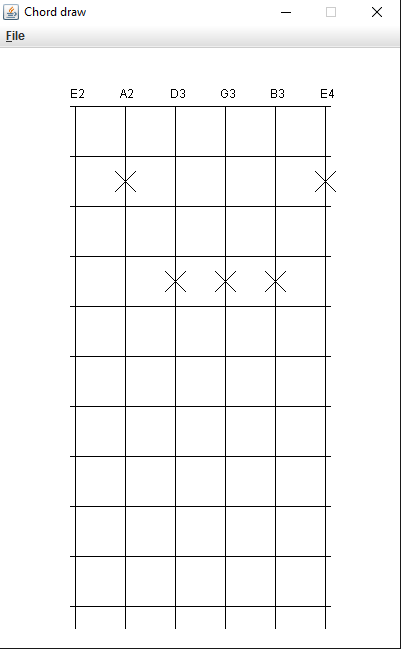
\includegraphics[width=0.5\textwidth]{../img/chords/ChordDraw}
%
% \Subtask Skapa en hjälpmetod \code{cross} som tar in två heltal $x$ och $y$. Metoden ska rita upp ett kryss som är 20x20 pixlar och har sitt centrum i den angivna koordinaten.
%
% \Subtask Rita ut ett kryss där en sträng trycks ner. \textbf{Tänk på att -1 och 0 anger att en sträng inte trycks ner}.
%
% \Subtask Implementera metoden \code{play} som börjar med att vänta på ett event från \code{SimpleWindow}, sedan kollar om eventet är av typen \code{SimpleWindow.MOUSE_EVENT}. Sedan ska man kolla om användaren tryckte på någon sträng (ett intervall på -10 till +10 i förhållande till strängens x-koordinat kan anses vara på strängen). Om användaren tryckt på en sträng ska denna spelas med hjälp av \code{SimpleNotePlayer}. Metoden \code{play} ska köras tills användaren kryssar ner fönstret, vilket motsvarar \code{SimpleWindow.CLOSE_EVENT}.
%
% \Subtask Lägg till menyvalet \code{draw} i \code{textui}. Använd \code{match} för att ta hand om felfallen att inget argument eller fler än ett argument angivits. Argumentet motsvarar ackordets plats i den filtrerade litan. Använd \code{Try} och \code{match} för att ta hand om felet att användaren anger något annat än en siffra. Använd \code{ChordDraw} för att rita upp ackord. \textbf{Kom ihåg att lägga till kommandot i listan med kommandon i \code{doCommand}}


%!TEX encoding = UTF-8 Unicode

%!TEX root = ../compendium1.tex

%!TEX encoding = UTF-8 Unicode
\chapter{Scala och Java}\label{chapter:W11}
Koncept du ska lära dig denna vecka:
\begin{multicols}{2}\begin{itemize}[nosep,label={$\square$},leftmargin=*]
\item skillnader mellan Scala och Java
\item klasser i Scala vs Java
\item referensvariabler vs enkla värden i Java
\item referenstilldelning vs värdetilldelning i Java
\item alternativ konstruktor i Scala och Java
\item for-sats i Java
\item java for-each i Java
\item java.util.ArrayList
\item autoboxing i Java
\item primitiva typer i Java
\item wrapperklasser i Java
\item samlingar i Java vs Scala
\item scala.collection.JavaConverters
\item översiktligt om relationen mellan trait och interface
\item namnkonventioner för konstanter
\item enum i java ???\end{itemize}\end{multicols}



%!TEX encoding = UTF-8 Unicode
%!TEX root = ../exercises.tex

\ifPreSolution



\Exercise{\ExeWeekELEVEN}\label{exe:W11}

\begin{Goals}
\item Kunna förklara och beskriva viktiga skillnader mellan Scala och Java.
\item Kunna översätta enkla algoritmer, klasser och singeltonobjekt från Scala till Java och vice versa.
\item Känna till vad en case-klass innehåller i termer av en Javaklass.
%\item Förstå hur autoboxing fungerar.
\item Kunna använda Javatyperna \code{List}, \code{ArrayList}, \code{Set}, \code{HashSet} och översätta till deras Scalamotsvarigheter med \code{CollectionConverters}.
\item Kunna förklara hur autoboxning fungerar i Java, samt beskriva fördelar och fallgropar.
\end{Goals}

\begin{Preparations}
\item \StudyTheory{11}
\end{Preparations}

\BasicTasks %%%%%%%%%%%%%%%%

\else



\ExerciseSolution{\ExeWeekELEVEN}

\BasicTasks %%%%%%%%%%%

\fi





\WHAT{Översätta metoder från Java till Scala.}

\QUESTBEGIN

\Task  \what~  I denna uppgift ska du översätta en Java-klass som används som en modul\footnote{\href{https://en.wikipedia.org/wiki/Modular_programming}{en.wikipedia.org/wiki/Modular\_programming}} och bara innehåller statiska metoder och inget förändringsbart tillstånd som kan ändras utifrån. (I nästa uppgift ska du sedan översätta klasser med förändringsbara  tillstånd.)

Vi börjar med att göra översättningen från Java till Scala rad för rad och du ska behålla så mycket som möjligt av syntax och semantik så att Scala-koden blir så Java-lik som möjligt. I efterföljande deluppgift ska du sedan omforma översättningen så att Scala-koden blir mer idiomatisk\footnote{\href{https://sv.wikipedia.org/wiki/Idiom_\%28programmering\%29}{sv.wikipedia.org/wiki/Idiom\_\%28programmering\%29}}.

\Subtask Studera klassen \code{Hangman} nedan. Du ska översätta den från Java till Scala enlig de riktlinjer och tips som följer efter koden. Läs igenom alla riktlinjer och tips innan du börjar.

\javainputlisting[numbers=left]{examples/scalajava/Hangman.java}

\noindent\emph{Riktlinjer och tips för översättningen:}

\begin{enumerate}[noitemsep]

\item Skriv Scala-koden med en texteditor i en fil som heter \texttt{hangman1.scala} och kompilera med \code{scalac hangman1.scala} i terminalen; använd alltså \emph{inte} en IDE, så som Eclipse eller IntelliJ, utan en ''vanlig'' texteditor, t.ex. VS \code{code}.

\item Översätt i denna första deluppgift rad för rad så likt den ursprungliga Java-kodens utseende (syntax)  som möjligt, med så få ändringar som möjligt. Du ska alltså ha kvar dessa Scalaovanligheter, även om det inte alls blir som man brukar skriva i Scala:
\begin{enumerate}[nolistsep, noitemsep]
\item långa indrag, \item onödiga semikolon, \item onödiga \code{()}, \item onödiga \code|{}|, \item onödiga \code{System.out}, och \item onödiga \code{return}.
\end{enumerate}

\item Försök också i denna deluppgift göra så att betydelsen (semantiken) så långt som möjligt motsvarar den i Java, t.ex. genom att använda \code{var} överallt, även där man i Scala normalt använder \code{val}.

\item En Javaklass med bara statiska medlemmar motsvarar ett singeltonobjekt i Scala, alltså en \code{object}-deklaration innehållande ''vanliga'' medlemmar.

\item För att tydliggöra att du använder Javas \code{Set} och \code{HashSet} i din Scala-kod, använd följande import-satser i \code{hangman1.scala}, som därmed döper om dina importerade namn och gör så att de inte krockar med Scalas inbyggda \code{Set}. Denna form av import går inte att göra i Java.
\begin{Code}
import java.util.{Set => JSet};
import java.util.{HashSet => JHashSet};
\end{Code}

\item Javas \code{i++} fungerar inte i Scala; man får istället skriva \code{i += 1} eller mindre vanliga \code{i = i + 1}.

\item Typparametrar i Java skrivs inom \code{<>} medan Scalas syntax för typparametrar använder \code{[]}.

\item Till skillnad från Java så har Scalas metoddeklarationer ett tilldelningstecken \code{=} efter returtypen, före kroppen.

\item Du kan ladda ner Java-koden till \code{Hangman}-klassen nedan från kursens repo%
\footnote{\href{https://github.com/lunduniversity/introprog/blob/master/compendium/examples/scalajava/Hangman.java}{github.com/lunduniversity/introprog/blob/master/compendium/examples/scalajava/Hangman.java}}. I samma bibliotek ligger även lösningarna till översättningen i Scala, men kolla \emph{inte} på dessa förrän du gjort klart översättningarna och fått dem att kompilera och köra felfritt! Tanken är att du ska träna på att läsa felmeddelande från kompilatorn och åtgärda dem i en upprepad kompilera-testa-rätta-cykel.

\end{enumerate}







\Subtask Skapa en ny fil \code{hangman2.scala} som till att börja med innehåller en kopia av din direkt-översatta Java-kod från föregående deluppgift. Omforma koden så att den blir mer som man brukar skriva i Scala, alltså mer Scala-idiomatisk. Försök förenkla och förkorta så mycket du kan utan att göra avkall på läsbarheten.

\emph{Tips och riktlinjer:}

\begin{enumerate}[nolistsep, noitemsep]

\item Kalla Scala-objektet för \code{hangman}. När man använder ett Scalaobjekt som en modul (alltså en samling funktioner i en gemensam, avgränsad namnrymd) har man gärna liten begynnelsebokstav, i likhet med konventionen för paketnamn. Ett paket är ju också en slags modul och med en namngivningskonvention som är gemensam kan man senare, utan att behöva ändra koden som använder modulen, ändra från ett singelobjekt till ett paket och vice versa om man så önskar.

\item Gör alla metoder publikt tillgängliga och låt även strängvektorn \code{hangman} vara publikt tillgänglig. Deklarera \code{hangman} som en \code{val} och konstruera den med \code{Vector}. Eftersom \code{Vector} är oföränderlig och man inte kan ärva från singelobjekt och \code{hangman} är deklarerad med \code{val} finns inga speciella risker med att göra den konstanta vektorn publik om  vi inte har något emot att annan kod kan läsa (och eventuellt göra sig beroende av) vår hänggubbetext.

\item I metoden \code{renderHangman}, använd \code{take} och \code{mkString}.

\item I metoden \code{hideSecret}, använd \code{map} i stället för en \code{for}-sats.

\item Det går att ersätta metoden \code{foundAll} med det kärnfulla uttrycket \\ \code{(secret forall found)} där \code{secret} är en sträng och \code{found} är en mängd av tecken (undersök gärna i REPL hur detta fungerar). Skippa därför den metoden helt och använd det kortare uttrycket direkt.

\item I metoden \code{makeGuess}, i stället för \code{Scanner}, använd \code{scala.io.StdIn.readLine}.

\item Om du vill träna på att använda rekursion i stället för imperativa loopar: Gör metoden \code{makeGuess} rekursiv i stället för att använda \code{do}-\code{while}.

\item I metoden \code{download}, i stället för \code{java.net.URL} och \code{java.util.ArrayList}, använd \code{scala.io.Source.fromURL(address, coding).getLines.toVector} och gör en lokal import av \code{scala.io.Source.fromURL} överst i det block där den används. Det går inte att ha lokala \code{import}-satser i Java.

\item Låt metoden \code{download} returnera en \code{Option[String]} som i fallet att nedladdningen misslyckas returnerar \code{None}.

\item I metoden \code{download}, i stället för \code{try}-\code{catch} använd \code{scala.util.Try} och dess smidiga metod \code{toOption}.

\item Om du vill träna på att använda rekursion i stället för imperativa loopar: Använd, i stället för \code{while}-satsen i metoden \code{play}, en lokal rekursiv funktion med denna signatur:
\begin{Code}
  def loop(found: Set[Char], bad: Int): (Int, Boolean)
\end{Code}
Funktionen \code{loop} returnerar en 2-tupel med antalet felgissningar och \code{true} om man hittat alla bokstäver eller \code{false} om man blev hängd.

\end{enumerate}





\SOLUTION


\TaskSolved \what
     %%%TODO number  1 %%%starts with: \emph{Översätta algoritmer och %%%

\SubtaskSolved  \scalainputlisting[numbers=left,basicstyle=\ttfamily\fontsize{10.3}{12}\selectfont]{examples/scalajava/hangman1.scala}

\SubtaskSolved  \scalainputlisting[numbers=left,basicstyle=\ttfamily\fontsize{11.2}{13}\selectfont]{examples/scalajava/hangman2.scala}



\QUESTEND






\WHAT{Översätta mellan klasser i Scala och klasser i Java.}

\QUESTBEGIN

\Task  \what~
Klassen \code{Point} nedan är en modell av en punkt som kan sparas på begäran i en lista. Listan är privat för kompanjonsobjektet och kan skrivas ut med en metod \code{showSaved}. I koden används en \code{ArrayBuffer}, men i framtiden vill man, vid behov, kunna ändra från \code{ArrayBuffer} till en annan sekvenssamlingsimplementation, t.ex. \code{ListBuffer}, som uppfyller egenskaperna hos supertypen \code{Buffer}, men har andra prestandaegenskaper för olika operationer. Därför är attributet \code{saved} i kompanjonsobjektet deklarerat med den mer generella typen.

\scalainputlisting[numbers=left]{examples/scalajava/Point.scala}

\Subtask Översätt klassen \code{Point} ovan från Scala till Java. Vi ska i nästa deluppgift kompilera både Scala-programmet ovan och ditt motsvarande Java-program i terminalen och testa i REPL att klasserna har motsvarande funktionalitet.

\emph{Tips och riktlinjer:}
\begin{enumerate}[nolistsep, noitemsep]
\item För att namnen inte ska krocka i våra kommande tester, kalla Javatypen för \code{JPoint}.
\item  I stället för Scalas \code{ArrayBuffer} och \code{Buffer}, använd Javas \code{ArrayList} och \code{List} som båda ligger i paketet \code{java.util}.
\item Undersök dokumentationen för \code{java.util.List} för att hitta en motsvarighet till \code{prepend} för att lägga till i början av listan.
\item I stället för default-argumentet i Scalas primärkonstruktor, använd en extra Java-konstruktor.
\item Det finns inga singelobjekt och inga kompanjonsobjekt i Java; istället kan man använda statiska klassmedlemmar. Placera kompanjonsobjektets medlemmars motsvarigheter \emph{inuti} Java-klassen och gör dem till \jcode{static}-medlemmar.
\item Kod i klasskroppen i Scalaklassen, så som if-satsen på rad 4, placeras i lämplig konstruktor i Javaklassen.
\item Utskrifter med \code{print} och \code{println} behöver i Java föregås av \code{System.out}.
\item Det finns inget nyckelord \code{override} i Java, men en s.k. annotering som ger samma kompilatorhjälp. Den skrivs med ett snabel-a och stor begynnelsebokstav, så här: \jcode{ @Override }  före metoddeklarationen.
\item I Java används konventionen att börja getter-metoder med ordet \code{get}, t.ex. \code{getX()}.
\item Det finns ingen motsvarighet till \code{mkString} för \code{List} så du behöver själv gå igenom listan och hämta elementreferenser för utskrift med en \jcode{for}-loop. Notera att efter sista elementet ska radbrytning göras i utskriften och att inget komma ska skrivas ut efter sista elementet.
\item I Java behövs en ny \jcode{import}-deklaration om man vill importera ännu en typ från samma paket. Man kan även i Java använda asterisk \code{*}, (motsvarande \code{_} i Scala), för att importera allt i ett paket, men då får man med alla möjliga namn och det vill man kanske inte.
\item Metoder i Java slutar med \code{()} om de saknar parametrar.
\item Alla satser i Java slutar med lättglömda semikolon. (Efter att man i skrivit mycket Javakod och växlar till Scalakod är det svårt att vänja sig av med att skriva semikolon...)
\end{enumerate}


\Subtask Starta REPL i samma bibliotek som du kompilerat kodfilerna. Testa så att klasserna \code{Point} och \code{JPoint} beter sig på samma vis enligt nedan. Skriv även testkod i REPL för att avläsa de attributvärden som har getters och undersök att allt funkar som det ska.
\begin{REPLnonum}
$ scalac Point.scala
$ javac JPoint.java
$ scala
scala> val (p, jp) = (new Point, new JPoint)
scala> p.distanceTo(new Point(3, 4))
scala> Point.showSaved
scala> jp.distanceTo(new JPoint(3, 4))
scala> JPoint.showSaved
scala> for (i <- 1 to 10) { new Point(i, i, true) }
scala> Point.showSaved
scala> for (i <- 1 to 10) { new JPoint(i, i, true) }
scala> JPoint.showSaved
\end{REPLnonum}


\Subtask Översätt nedan Javaklass \code{JPerson} till en \code{case class Person} i Scala med  motsvarande funktionalitet.


\javainputlisting[numbers=left]{examples/scalajava/JPerson.java}


\Subtask\Pen Undersök i REPL vilken funktionalitet i Scala-case-klassen \code{Person} som \emph{inte} är implementerad i Java-klassen \code{JPerson} ovan. Skriv upp namnen på några av case-klassens extra metoder samt deras signatur genom att för en \code{Person}-instans, och för kompanjonsobjektet \code{Person}, trycka på TAB-tangenten. Prova några av de extra metoderna i REPL och förklara vad de gör.

\begin{REPL}
scala> val p = Person("Björn", 49)
scala> p.      // tryck TAB en gång
scala> Person. // tryck TAB en gång
scala> p.copy  // tryck TAB en gång
scala> p.copy()
scala> p.copy(age = p.age + 1)
scala> Person.unapply(p)
\end{REPL}


\SOLUTION


\TaskSolved \what
     %%%TODO number  2 %%%starts with: \emph{Översätta mellan klasser %%%

\SubtaskSolved   \javainputlisting[numbers=left]{examples/scalajava/JPoint.java}

\SubtaskSolved   -

\SubtaskSolved   \begin{Code}
case class Person(name: String, age: Int = 0)
\end{Code}

\SubtaskSolved  p.*TAB* - copy, producArity, ProductIterator, productElement, productPrefix

Person.*TAB* - apply, curried, tupled, unapply

\begin{REPLnonum}
scala> p.copy
   def copy(name: String,age: Int): Person

scala> p.copy()
res0: Person = Person(Björn,49)

scala> p.copy(age = p.age + 1)
res1: Person = Person(Björn,50)

scala> Person.unapply(p)
res2: Option[(String, Int)] = Some((Björn,49))
\end{REPLnonum}



\QUESTEND






\WHAT{Auto(un)boxing.}

\QUESTBEGIN

\Task  \what~  I JVM måste typparametern för generiska klasser vara av referenstyp. I Scala löser kompilatorn detta åt oss så att vi ändå kan ha t.ex. \code{Int} som argument till en typparameter i Scala, medan man i Java \emph{inte} direkt kan ha den primitiva typen \jcode{int} som typparameter till t.ex. \code{ArrayList}.

I Java och i den underliggande plattformen JVM används s.k. wrapper-klasser för att lösa detta, t.ex. genom wrapper-klassen \code{Integer} som boxar den primitiva typen \jcode{int}. Java-kompilatorn har stöd för att automatiskt packa in värden av primitiv typ i sådana wrapper-klasser för att skapa referenstyper och kan även automatiskt packa upp dem.

\Subtask Studera hur Scala-kompilatorn låter oss arbeta med en \code{Cell[Int]} även om det underliggande JVM:ens körtidstyp \Eng{runtime type} är en wrapper-klass. Man kan se JVM-körtidstypen med metoderna \code{getClass} och \code{getTypeName} enligt nedan.
\begin{REPL}
scala> class Cell[T](var value: T){
         val typeName: String = value.getClass.getTypeName
         override def toString = "Cell[" + typeName + "](" + value + ")"
       }
scala> val c = new Cell[Int](42)
scala> c.value.getClass.getTypeName
\end{REPL}


\Subtask Vad är körtidstypen för \code{c.value} ovan? Förklara hur det kan komma sig trots att vi deklarerade med typargumentet \code{Int}?

\Subtask Studera dokumentationen för \code{java.lang.Integer}\footnote{\href{https://docs.oracle.com/javase/8/docs/api/java/lang/Integer.html}{docs.oracle.com/javase/8/docs/api/java/lang/Integer.html}} och testa i REPL några av \emph{klassmetoderna} (de som är \jcode{static} och därmed kan anropas med punktnotation direkt på klassens namn utan \code{new}) och några av \emph{instansmetoderna} (de som inte är \jcode{static}).
\begin{REPL}
scala> Integer.  //tryck TAB
scala> Integer.
scala> Integer.toBinaryString(42)
scala> Integer.valueOf(42)
scala> val i = new Integer(42)
scala> i.  // tryck TAB
scala> i.toString
scala> i.compareTo  // tryck TAB 2 gånger
scala> i.compareTo(Integer.valueOf(42))
scala> i.compareTo(42)  // varför fungerar detta?
\end{REPL}

\Subtask\Pen Enligt dokumentationen\footnote{\href{https://docs.oracle.com/javase/8/docs/api/java/lang/Integer.html\#compareTo-java.lang.Integer-}{docs.oracle.com/javase/8/docs/api/java/lang/Integer.html\#compareTo-java.lang.Integer-}} tar instansmetoden \code{compareTo} i klassen \code{Integer} en \code{Integer} som parameter. Hur kan det då komma sig att sista raden ovan fungerar med en \code{Int}?

\Subtask Studera nedan Java-program och beskriv vad som kommer att skrivas ut \emph{innan} du kompilerar och testkör.

\javainputlisting[numbers=left]{examples/scalajava/Autoboxing.java}

\Subtask Ändra i programmet ovan så att autoboxing och autounboxing utnyttjas på alla ställen där så är möjligt. Utnyttja även att \code{toString}-metoden på \code{Integer} ger samma stränrepresentation som \jcode{int} vid utskrift. Fixa också så att du undviker \emph{fallgropen} att i Java jämföra med referenslikhet i stället för att använda \code{equals}. Testa så att allt fungerar som det borde efter dina ändringar.


\Subtask\Pen Antag att du råkar skriva \jcode{xs.add(0, pos)} på rad 14 i ditt program från föregående uppgift. Förklara hur autoboxingen stjälper dig i en \emph{fallgrop} då.

\Subtask\Pen Med ledning av de båda tidigare deluppgifterna: sammanfatta de två nämnda fallgropar med autoboxing i Java i två generella punkter, så att du har nytta av att memorera dem inför din framtida Javakodning.


\SOLUTION


\TaskSolved \what
     %%%TODO number  3 %%%starts with: \emph{Auto(un)boxing.} I JVM må%%%

\SubtaskSolved   -

\SubtaskSolved   Cell har typen java.lang.Integer. När man hämtar ut värdet med \code{c.value} hämtas den primitiva typ \code{int} ut.

\SubtaskSolved   Med hjälp av autoboxing förvandlas 42 till typen \code{Integer} och kan därför jämföras med en annan \code{Integer}.

\SubtaskSolved   i.compareTo(42) fungerar på grund av autoboxing. Då JVM packar in den primitiva typ int i en Integer-objekt automatiskt.

\SubtaskSolved
\begin{REPLnonum}
0 10 20 30 40 50 60 ... 390 400 410

[0]: 0
[42]: 0
NOT EQUAL
\end{REPLnonum}

\SubtaskSolved   \javainputlisting[numbers=left]{examples/scalajava/Autoboxing2.java}

\SubtaskSolved   42 kommer läggas längst fram i listan istället för längst bak, då autounboxing kommer göra Integer(0) till 0 och tvärtom med variablen \code{pos}.

\SubtaskSolved   Om man ska undersöka om två int-variabler är lika ska man använda ==, men om variablerna är av typen Integer måste man använda \code{equals}.

JVM kommer inte varna om man vänder på \code{Integer} och \code{int}, som i \code{xs.add(0, pos)}.



\QUESTEND






\WHAT{JavaConverters.}

\QUESTBEGIN

\Task  \what~  Med \code{import scala.jdk.CollectionConverters._} får man i sina Scalaprogram tillgång till de smidiga metoderna \code{asJava} och \code{asScala} som översätter mellan motsvarande samlingar i resp språks standardbibliotek. Kör nedan i REPL och gör efterföljande deluppgifter.

\begin{REPL}
scala> val sv = Vector(1,2,3)
scala> val ss = Set('a','b','c')
scala> val sm = Map("gurka" -> 42, "tomat" -> 0)
scala> val ja = new java.util.ArrayList[Int]
scala> ja.add(42)
scala> val js = new java.util.HashSet[Char]
scala> js.add('a')
scala> import scala.jdk.CollectionConverters._
\end{REPL}

\Subtask Till vilka typer konverteras Scalasamlingarna
\code{Vector[Int]}, \code{Set[Char]} och \\ \code{Map[String, Int]} om du anropar metoden \code{asJava} på dessa?

\Subtask Till vilka typer konverteras Javasamlingarna \code{ArrayList[Int]} och \code{HashSet[Char]}  om du anropar metoden \code{asScala} på dessa? Blir det föränderliga eller oföränderliga motsvarigheter?

\Subtask Vad får resultatet för typ om du kör \code{toSet} på en samling av typen \code{mutable.Set}?

\Subtask Undersök hur du kan efter att du gjort \code{sm.asJava.asScala} anropa ytterligare en metod för att få tillbaka en oföränderlig \code{immutable.Map}.

\Subtask Läs mer i dokumentationen om JavaConverters\footnote{\href{http://docs.scala-lang.org/overviews/collections/conversions-between-java-and-scala-collections.html}{docs.scala-lang.org/overviews/collections/conversions-between-java-and-scala-collections.html}}
och prova några fler konverteringar.



\SOLUTION


\TaskSolved \what
     %%%TODO number  4 %%%starts with: \emph{JavaConverters.} Med \cod%%%

\SubtaskSolved

Vector[Int] -> java.util.List[Int]

Set[Char] -> java.util.Set[Char]

Map[String, Int] -> java.util.Map[String, Int]

\SubtaskSolved

ArrayList[Int] -> scala.collection.mutable.Buffer[Int]

HashSet[Char] -> scala.collection.mutable.Set[Char]

Båda blir föränderliga motsvarigheter. Det visas genom att de till hör \code{scaka.collection.mutable} och både \code{ArrayList} och \code{HashSet} är förändrliga i Java.

\SubtaskSolved   \code{scala.collection.immutable.Set}

\SubtaskSolved   \code{sm.asJava.asScala} ger typen \code{scala.collection.mutable.Map[String,Int]}

\code{sm.asJava.asScala.toMap} ger typen \code{scala.collection.immutable.Map[String,Int]}

\SubtaskSolved   -

\QUESTEND




\ExtraTasks %%%%%%%%%%%%%%%%%%%


\WHAT{Översätta från Java till Scala.}

\QUESTBEGIN

\Task  \what~ Översätt nedan kod från Java till Scala. Skriv koden i en fil som heter \texttt{showInt.scala} och kalla Scala-objektet med \code{main}-metoden för \code{showInt}. Läs tipsen som följer efter koden innan du börjar.

\javainputlisting[numbers=left]{examples/scalajava/JShowInt.java}

\emph{Tips:}
\begin{itemize}[nolistsep, noitemsep]
\item En Javaklass med bara statiska medlemmar motsvaras av ett singeltonobjekt i Scala, alltså en \code{object}-deklaration. Scala har därför inte nyckelordet \jcode{static}.
\item Typen \jcode{Object} i Java motsvaras av Scalas \code{Any}.
\item Du kan använda Scalas möjlighet med default-argument (som saknas i Java) för att bara definiera en enda \code{show}-metod med en tom sträng som default \code{msg}-argument.
\item I Scala har objekt av typen \code{Char} en metod \code{def *(n: Int): String} som skapar en sträng med tecknet repeterat \code{n} gånger. Men du kan ju välja att ändå implementera metoden \code{repeatChar} med \code{StringBuilder} som nedan om du vill träna på att översätta en \code{for}-loop från Java till Scala.
\item I stället för \code{Scanner.nextLine} kan du använda \code{scala.io.StdIn.readLine} som tar en prompt som parameter, men du kan också använda \code{Scanner} i Scala om du vill träna på det.
\item I Java \emph{måste} man använda nyckelordet \jcode{return} om metoden inte är en \jcode{void}-metod, medan man i Scala faktiskt \emph{får} använda \code{return} även om man brukar undvika det och i stället utnyttja att satser i Scala också är uttryck.
\end{itemize}
Kompilera din Scala-kod och kör i terminalen och testa så att allt funkar. Vill du även kompilera Java-koden så finns den i kursens repo i filen\\ \texttt{compendium/examples/scalajava/JShowInt.java}


\SOLUTION


\TaskSolved \what


\begin{Code}[numbers=left]
object showInt {
  def show(obj: Any, msg: String = ""): Unit = println(msg + obj)

  def repeatChar(ch: Char, n: Int): String = ch.toString * n

  def showInt(i: Int): Unit = {
    val leading = Integer.numberOfLeadingZeros(i)
    val binaryString = repeatChar('0', leading) + i.toBinaryString
    show(i,               "Heltal : ")
    show(i.asInstanceOf[Char],         "Tecken : ")
    show(binaryString,    "Binärt : ")
    show(i.toHexString,   "Hex    : ")
    show(i.toOctalString, "Oktal  : ")
  }


  import scala.io.StdIn.readLine
  import scala.util.{Try,Success,Failure}

  def loop: Unit =
    Try { readLine("Heltal annars pang: ").toInt } match {
      case Failure(e) => show(e); show("PANG!")
      case Success(i) => showInt(i); loop
    }

  def main(args: Array[String]): Unit =
    if(args.length > 0) args.foreach(i => showInt(i.toInt))
    else loop
}
\end{Code}



\QUESTEND






\WHAT{Innehållslikhet och referenslikhet i Java.}

\QUESTBEGIN

\Task  \what~ Studera och prova denna fallgrop med innehållslikhet: \href{https://github.com/bjornregnell/lth-eda016-2015/blob/master/lectures/examples/eclipse-ws/lecture-examples/src/week10/generics/TestPitfall3.java}{TestPitfall3.java}







\SOLUTION


\TaskSolved \what
     %%%TODO number  6 %%%starts with: \TODO Fallgrop med Point som in%%%



\QUESTEND




\AdvancedTasks %%%%%%%%%%%%%%%%%


\WHAT{Implementera innehållslikhet i Java.}

\QUESTBEGIN

\Task  \what~\Pen Studera fallgropar för hur man skriver en \code{equals}-metod i Java här:
\href{http://www.artima.com/lejava/articles/equality.html}{www.artima.com/lejava/articles/equality.html} och jämför med  det fullständiga receptet för hur man skriver en välfungerande \code{equals} och \code{hashcode} i Scala här: \href{http://www.artima.com/pins1ed/object-equality.html}{www.artima.com/pins1ed/object-equality.html}

\Subtask Vilka skillnader och likheter finns vid överskuggning av equals i Java respektive Scala, som ska ge en fungerande innehållstest för en hierarki med bastyper och subtyper?

\Subtask Vilka fallgropar är gemensamma för Java och Scala?\SOLUTION


\TaskSolved \what
     %%%TODO number  7 %%%starts with: \TODO \emph{Gränssnitt i Scala %%%



\QUESTEND

%!TEX encoding = UTF-8 Unicode
%!TEX root = ../compendium2.tex

\Lab{\LabWeekELEVEN}

\begin{Goals}
\item Förstå skillnaden mellan primitiva typer och objekt i Java.
\item Kunna förklara hur autoboxing fungerar i Java.
\item Kunna förklara vad statiska metoder och attribut i Java innebär.
\item Kunna använda \code{ArrayList} och arrayer i Java.
\item Kunna använda Java-klassen \code{Scanner}.
\item Kunna skapa en for-sats i Java.
\item Känna till hur man kan förenkla användandet av Java och Scala i samma program med hjälp av \code{scala.collection.JavaConverters}.
\end{Goals}

\begin{Preparations}
\item \DoExercise{\ExeWeekELEVEN}{11}
\item Studera given kod här: \url{https://github.com/lunduniversity/introprog/tree/master/workspace/w11_javatext/}
\end{Preparations}

\subsection{Krav}

Du ska skapa ett textspel för terminalen som är (lagom) intressant/roligt att spela, sparar poäng per spelomgång för olika spelare och mäter tiden det tog att spela. Till din hjälp har du den färdiga filen \code{Main.java} (som går bra att förändra om det behövs) samt de två kodskeletten \code{Game.java} och \code{UserInterface.scala}. Ditt textspel ska köras i terminalen och uppfylla följande krav och riktlinjer:

\begin{enumerate}
  \item När ditt program kör ska man ska kunna starta flera spelomgångar efter varandra utan att behöva avsluta programmet.
  \item För varje spelomgång ska programmet komma ihåg spelarens namn\footnote{eller spelar\emph{nas} namn om det är ett spel för två eller flera personer} med tillhörande resultat.
  \item Efter begäran ska programmet kunna visa en topplista med bästa poäng, både för alla spelare och för ett specifikt spelarnamn.
%  \item Speltiden för varje spelomgång ska mätas och sparas tillsammans med poängresultatet för respektive spelare.
  \item Koden för själva spelet ska vara skriven i Java, men Scala ska användas för att implementera funktionerna i singelobjektet \code{UserInterface}.
  \item I Scala-koden ska du för träningens skull använda Java-klassen \code{java.util.Scanner} när du läser in data från terminalen.
  \item Koden i singelobjektet \code{UserInterface} ska använda omvandlingsmetoden \code{asScala} efter \code{import scala.collection.JavaConverters._} för att omvandla argument av typen \code{java.util.ArrayList}.
  \item Ditt spel ska i Java-kod använda minst en av datastrukturerna
  \code{ArrayList},
  \code{HashSet},
  \code{HashMap} ur paketet \code{java.util}, samt minst en array. (Den givna koden i \code{Main.java} räknas inte till detta krav.)
  \item Du ska spela någon annans halvfärdiga spel och, efter att du studerat koden, ge återkoppling på kodens läsbarhet.
  \item Du ska låta någon annan spela ditt halvfärdiga spel och visa din kod och fråga om återkoppling på läsbarheten. Du ska anteckna den återkoppling du får.
  \item Du ska inför redovisningen förbereda följande:
  \begin{enumerate}
    \item en kort genomgång av spelets idé,
    \item en kort förklaring av kodens struktur och de olika Java-klassernas ansvar,
    \item en kort redogörelse för den återkoppling du fått på din kods läsbarhet och hur du arbetat med att förbättra läsbarheten under dina stegvisa utvidgningar av din kod,
    \item en lista med koncept som du tränat på när du skapat ditt textspel.
  \end{enumerate}
\end{enumerate}

\subsection{Frivilliga extrauppgifter}

\begin{enumerate}
	\item Spara resultat i en fil efter varje spelomgång, och läs in resultat från filen antingen när programmet startas eller när användaren vill se poänglistan, så att det går att se spelresultat från tidigare körningar av programmet. Den kod du behöver lägga till för att åstadkomma detta kan vara skriven antingen i Java eller Scala. Tänk på att du kan behöva göra ändringar även i \code{Main}-klassen.
	\item   Mät speltiden för varje spelomgång och spara tiden tillsammans med poängresultatet för respektive spelare.

\end{enumerate}

\subsection{Inspiration och tips}

\begin{enumerate}
  \item Utgå från Hangman i veckans övning eller,
  \item Yatzy från tidigare övningar, eller
  \item skapa ett kortspel inspirerat av \code{shuffle}-labben, eller
  \item inspireras av listan med sällskapsspel på wikipedia:\\ \href{https://sv.wikipedia.org/wiki/Kategori:Sällskapsspel}{sv.wikipedia.org/wiki/Kategori:Sällskapsspel}
  \item eller hitta på ett eget textspel.
  \item Börja med en starkt förenklad variant som du sedan bygger vidare på.
  \item Kompilera och testa efter varje ändring, så att du hela tiden har ett fungerande program.
  \item Dela upp din spelkod i flera metoder, och även flera klasser om det är lämpligt.
  \item Det finns mycket information på nätet om hur man skriver Java-kod och använder JDK, t.ex. på \url{https://stackoverflow.com/}
  \item Träna på att använda JDK-dokumentationen här:\\ \url{https://docs.oracle.com/javase/8/docs/api/}
\end{enumerate}


%!TEX encoding = UTF-8 Unicode

%!TEX root = ../compendium1.tex

\chapter{Trådar, Web, Android}
\begin{itemize}[nosep]
\item Thread
\item Future
\item HTML
\item Javascript
\item css
\item Scala.js
\item Android
\end{itemize}
\clearpage
%!TEX encoding = UTF-8 Unicode
%!TEX root = ../lect-week11.tex

%%%

\ifkompendium\else

\Subsection{Veckans labb: \texttt{survey2}}
\begin{Slide}{Veckans labb: \texttt{survey2}}\SlideFontTiny
\begin{minipage}{0.65\textwidth}
Nya version 2 av labben är enklare och kräver ej att du implementerar parsning av \code{args}. Välj själv vilken du gör.

\vspace{0.5em}
\Emph{Förberedelse:}
\begin{itemize}
\item Studera givna koden: {\SlideFontTiny \href{https://github.com/lunduniversity/introprog/tree/master/workspace/w10_survey2/src/main/scala/stats}{workspace/w10\_survey2}}
\item Fyll i denna enkät:
\\{\SlideFontTiny \url{https://goo.gl/forms/hC6JK2UQXVpbGECc2}} 
\end{itemize}

\Emph{Grunduppgift:}
\begin{itemize}
\item Implementera en klass \code{Table} för hantering av strängmatriser med rubrikrad från kolumnsepararade textfiler.
\item Öva på att kombinera matriser, sortering, registrering för att räkna statistik.
\item Använda inbyggda sorteringsfunktioner: \\\code{sortBy} och \code{sortWith}
\item Implementera din egen sortering ''från scratch''.
\end{itemize}
\Emph{Extrauppgift:}
\begin{itemize}
\item Implementera stapeldiagram.
\end{itemize}
\end{minipage}
\hfill\begin{minipage}{0.27\textwidth}
\centering
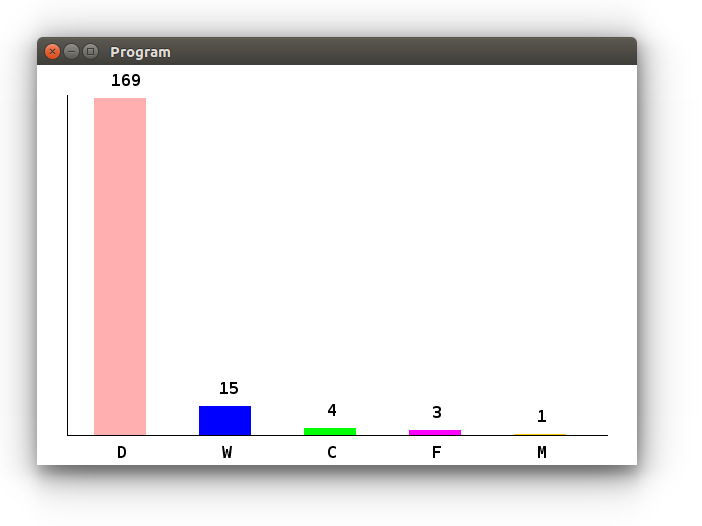
\includegraphics[width=0.9\textwidth]{../img/survey/bar}

\vspace{2em}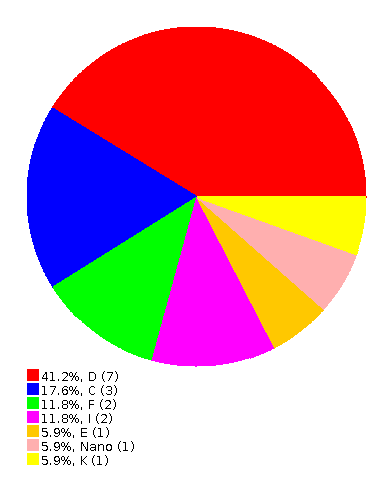
\includegraphics[width=0.7\textwidth]{../img/survey/pie}
\end{minipage}
\end{Slide}


\fi












%!TEX encoding = UTF-8 Unicode
%!TEX root = ../lect-w12.tex

%%%


\Subsection{Repetition: Vad är en algoritm?}
\begin{Slide}{Repetition: Vad är en algoritm? }\SlideFontTiny
\pause En \href{https://sv.wikipedia.org/wiki/Algoritm}{algoritm} är en stegvis beskrivning av hur man löser ett problem. \\ 
Exempel: SWAP, MIN, Registrering, Sökning, Sortering \\
\pause\vspace{0.5em}
Problemlösningsprocessens olika steg (inte nödvändigtvis i denna ordning): 
\begin{itemize}
\item Dela upp problemet i enklare delproblem och sätt samman.
\item Finns redan färdig lösning på (del)problem?
\item Formulera (del)\Emph{problemet} och ange tydligt indata och utdata: \\ exempel MIN: indata: sekvens av heltal; utdata: minsta talet
\item Kom på en \Emph{lösningsidé}: (kan  vara mycket klurigt och svårt) \\ exempel MIN: iterera över talen och håll reda på ''minst hittills''
\item Formulera en \Emph{stegvis beskrivning} som löser problemet: \\ exempel: pseudo-kod med sekvens av instruktioner
\item Implementera en \Emph{körbar lösning} i ''riktig'' kod: \\ exempel: en Scala-metod i en klass eller i ett singelobjekt
\item Har algoritmen acceptabel komplexitet i förhållande till tids- och minneskrav?
\end{itemize}
\pause Det krävs ofta \Emph{kreativitiet} i stegen ovan  -- även i att \Emph{känna igen} problemet!\\
Simpelt exempel: Du stöter på problemet MAX och ser likheten med MIN.\\
\pause\vspace{0.5em}\Emph{Övning}: Diskutera hur du löser detta problem i relation till stegen ovan: \\
\emph{Att räkna antalet förekomster av olika unika ord i en textsträng.} 
\end{Slide}













%!TEX encoding = UTF-8 Unicode
%!TEX root = ../lect-week11.tex

%%%

\ifkompendium\else

\Subsection{Jämföra strängar}

\begin{Slide}{Att jämföra strängar lexikografiskt}\SlideFontSmall
Teckenstandard \href{https://sv.wikipedia.org/wiki/UTF-16}{UTF-16}: Alla stora bokstäver är ''mindre'' än alla små:
\begin{REPLnonum}
scala> Array("hej","Hej","gurka").sorted
\end{REPLnonum}
\pause\vspace{-1.2em}
\begin{REPLnonum}
res0: Array[String] = Array(Hej, gurka, hej)\end{REPLnonum}
\pause
\begin{itemize}
\item Antag att vi vill lösa detta problem ''från scratch'': \\ \Emph{att sortera en sekvens med strängar} 
\item För att göra detta behöver vi lösa dessa delproblemen: 
\begin{itemize}
\item \Emph{att} \Alert{jämföra strängar}
\item \Emph{sökning i sekvenser}
\item \Emph{SWAP} (om på-plats-sortering i förändringsbar sekvens)
\end{itemize}
\item Vad betyder det att två strängar är ''lika''?

\item Vad betyder det att en sträng är ''mindre'' än en annan?
\end{itemize}
\pause {\SlideFontTiny Vi använder här strängjämförelse, sökning och sortering för att illustrera typiska \Emph{imperativa algoritmer}. \Alert{Normalt} använder man \Emph{färdiga lösningar} på dessa problem!}

\end{Slide}

\begin{Slide}{Jämföra strängar: likhet}\SlideFontSmall
Antag att vi inte kan göra \code{s1 == s2} utan bara kan jämföra strängar tecken för tecken, 
t.ex. så här: \code{s1(i) == s2(i)}. Antag också att vi inte har tillgång till annat än metoderna \code{length} och \code{apply} på strängar, samt  \code{while} och variabler av grundtyp. \Emph{Lös problemet att \emph{avgöra om två strängar är lika}.}

\pause
\begin{itemize}
\item Indata: två strängar
\item Utdata: \code{true} om lika annars \code{false}
\end{itemize}
\begin{enumerate}
\item Klura ut din lösningsidé
\item Formulera algoritmen i pseudokod
\item Implementera algoritmen i Scala: \code{def isEqual(s1: String, s2: String): Boolean} = ???
\end{enumerate}
\end{Slide}

\begin{Slide}{Algoritmexempel: stränglikhet, pseudokod}
\begin{Code}
def isEqual(s1: String, s2: String): Boolean = {
  if (/* lika längder */) {
    var foundDiff = false
    var i = /* första index */
    while (!foundDiff && /* i inom indexgräns */) {
      if (/* tecken på plats i är olika */) foundDiff = true
      else i = /* nästa index */
    }
    !foundDiff
  } else false
}
\end{Code}

\pause Detta är en variant av s.k. \Emph{linjärsökning} där vi söker från början i en sekvens till vi hittar det vi söker efter (här söker vi efter tecken som skiljer sig åt). 
\\\pause\vspace{2.5em} Hur ser implementationen i exekverbar Scala ut?
\end{Slide}

\begin{Slide}{Algoritmexempel: stränglikhet, implementation}\SlideFontSmall
\begin{Code}
def isEqual(s1: String, s2: String): Boolean = {
  if (s1.length == s2.length) {
    var foundDiff = false
    var i = 0
    while (!foundDiff && i < s1.length) {
      if (s1(i) != s2(i)) foundDiff = true
      else i += 1
    }
    !foundDiff
  } else false
}
\end{Code}
\pause 
{\SlideFontTiny Fördjupning: jämför ovan med implementationen av \code{String.equals} här:
\href{http://hg.openjdk.java.net/jdk8u/jdk8u60/jdk/file/935758609767/src/share/classes/java/lang/String.java#l976}{hg.openjdk.java.net/jdk8u/jdk8u60/jdk/file/935758609767/src/share/classes/java} \\ och använd \code{timed} nedan och jämför prestanda med \code{isEqual} ovan.\\
Obs! Mät många gånger så att JVM:en optimerar din kod.}
\vspace{-0.25em}\begin{Code}
def timed[T](block: => T): (Double, T) = { 
  val (t, res) = (System.nanoTime, block)
  ((System.nanoTime - t) / 1e9, res) 
}
\end{Code}

\end{Slide}

\begin{Slide}{Algoritmexempel: stränglikhet, prestanda}
\begin{REPL}
scala> val enMiljon = 1000000

scala> val s = Array.fill(enMiljon)('x').mkString

scala> val t = s.updated(enMiljon - 1, 'y')

scala> timed { s == t }
res42: (Double, Boolean) = (3.76459E-4,false)

scala> timed { isEqual(s,t) } 
res43: (Double, Boolean) = (3.31597E-4,false)
\end{REPL}
Ovan är kört efter ''uppvärmning'' på i7-4790K CPU @ 4.00GHz \\
Skillnaden inom mätfelmarginalen!
\end{Slide}



\begin{Slide}{Jämföra strängar: ''mindre än''}\SlideFontSmall
Med \code{s1 < s2} menar vi att strängen s1 ska sorteras före strängen s2 enligt hur de enskilda tecknen är ordnade med uttrycket \code{s1(i) < s2(i)}. \\
Antag också att vi inte har tillgång till annat än metoderna \code{length} och \code{apply} på strängar, samt  \code{while} och variabler av grundtyp, samt \code{math.min}
\\\Emph{Lös problemet att \emph{avgöra om en sträng är ''mindre'' än en annan}.}\\
\begin{itemize}
\item Indata: två strängar, s1, s2
\item Utdata: \code{true} om s1 ska sorteras före s2 annars \code{false}
\end{itemize}
\begin{enumerate}
\item Klura ut din lösningsidé
\item Formulera algoritmen i pseudokod
\item Implementera algoritmen i Scala: \code{def isLessThan(s1: String, s2: String): Boolean} = ???
\end{enumerate}
\end{Slide}

\begin{Slide}{Jämföra strängar: ''mindre än''}\SlideFontSmall
Pseudokod:
\begin{Code}
def isLessThan(s1: String, s2: String): Boolean = {
  
  val minLength = /* minimum av längderna på s1 och s2 */
  
  def firstDiff(s1: String, s2: String): Int = 
    /* index för första skillnaden (om de börjar lika: minLength) */

  val diffIndex = firstDiff(s1, s2)
  if (diffIndex == minLength) /* s1 är kortare än s2 */
  else /* tecknet s1(diffIndex) är mindre än tecknet s2(diffIndex) */ 
}
\end{Code}
\end{Slide}

\begin{Slide}{Jämföra strängar: ''mindre än''}\SlideFontSmall
\begin{Code}
def isLessThan(s1: String, s2: String): Boolean = {

  val minLength = math.min(s1.length, s2.length)

  def firstDiff(s1: String, s2: String): Int = {
    var foundDiff = false
    var i = 0
    while (!foundDiff && i < minLength) 
      if (s1(i) != s2(i)) foundDiff = true 
      else i += 1
    i
  }

  val diffIndex = firstDiff(s1, s2)
  if (diffIndex == minLength) s1.length < s2.length
  else s1(diffIndex) < s2(diffIndex)
}
\end{Code}
\end{Slide}

\begin{Slide}{Jämföra strängar i Java}\SlideFontTiny
\begin{itemize}
\item I Java kan man \Alert{inte} jämföra strängar med operatorerna \code{<}, \code{<=}, \code{>}, och \code{>=}

\item Dessutom ger operatorerna \code{==} och \code{!=} \emph{inte} innehålls(o)likhet utan \Alert{referens(o)likhet} \code{:(}

\item Istället \Alert{måste} man i Java använda metoderna \code{equals} och \code{compareTo} 
\\Dessa fungerar även i Scala eftersom strängar i Scala och Java är av samma typ, nämligen \code{java.lang.String}.
\pause
\item \code{s1.compareTo(s2)} ger ett heltal som är:
\begin{itemize}\SlideFontTiny
\item \code{0} om s1 och s2 har samma innehåll
\item \Alert{negativt} om s1 < s2 i lexikografisk mening, alltså s1 ska sorteras \Alert{före}
\item \Emph{positivt} om s1 > s2 i lexikografisk mening, alltså s1 ska sorteras \Emph{efter}
\end{itemize}

\pause
\item Undersök följande:
\begin{REPL}
scala> new String("hej") eq new String("hej") // motsvarar == i Java
scala> "hej".equals("hej")                    // samma som == i Scala
scala> "hej".compareTo("hej")
scala> "hej".compareTo("HEJ")         // alla stora är 'före' alla små
scala> "HEJ".compareTo("hej")
\end{REPL}
\end{itemize}

\href{http://docs.oracle.com/javase/8/docs/api/java/lang/String.html#compareTo-java.lang.String-}{docs.oracle.com/javase/8/docs/api/java/lang/String.html\#compareTo-java.lang.String-}
\end{Slide}


\begin{Slide}{Jämföra strängar i Java: exempel}\SlideFontSmall
Vad skriver detta Java-program ut?
\javainputlisting{../compendium/examples/StringEqTest.java}
\pause
\begin{REPL}
$ javac StringEqTest.java 
$ java StringEqTest 
false
true
0
\end{REPL}
\end{Slide}


\fi












%!TEX encoding = UTF-8 Unicode
%!TEX root = ../lect-week11.tex

%%%

\ifkompendium\else

\Subsection{Jämförelse Scala och Java}
\begin{Slide}{Grundläggande likheter och skillnader}\SlideFontSmall

\begin{itemize}
\item \Emph{Sökning} återkommer i många skepnader: \\ i en datastruktur, vilken det än må vara, vill man ofta kunna \\ \Emph{hitta ett element med en viss egenskap}. 

\pause
Några färdiga linjärsökningar i Scalas standardbibliotek:

\begin{REPL}
scala> Vector("gurka","tomat","broccoli").indexOf("tomat")
res0: Int = 1

scala> Vector("gurka","tomat","broccoli").indexWhere(_.contains("o"))
res1: Int = 1

scala> Vector("gurka","tomat","broccoli").find(_.contains("o"))
res2: Option[String] = Some(tomat)
\end{REPL}

\pause
\item Sökning efter ett visst index i en sekvens:

\begin{itemize}\SlideFontTiny
\item Indata: en sekvens och ett \Emph{sökkriterium}
\item Utdata: index för första eftersökta element, annars -1 
\end{itemize}

\pause
\item Två typiska varianter av sökning i en sekvens:
\begin{itemize}\SlideFontTiny
\item Linjärsökning: börja från början och sök tills ett eftersökt element är funnet
\item Binärsökning: antag sorterad sekvensen; börja i mitten, välj rätt halva ...
\end{itemize}
\end{itemize}
\end{Slide}

\Subsection{Linjärsökning}

\begin{Slide}{Linjärsökning: hitta index för elementet 42}
Skriv pseudokod för:\\ \code{def indexOf42(xs: Vector[Int]): Int = ???}
\pause
\begin{Code}
def indexOf42(xs: Vector[Int]): Int = {
  var i = /* index för första elementet */
  var found = false
  while (!found && /* index inom indexgräns */) {
    if (/* element på plats i är 42 */) found = true 
    else i = /* nästa index */
  }
  if (/* hittat */) i else -1
} 
\end{Code}
\end{Slide}

\begin{Slide}{Linjärsökning: hitta index för elementet 42}
Implementera:\\ \code{def indexOf42(xs: Vector[Int]): Int = ???}
\pause
\begin{Code}
def indexOf42(xs: Vector[Int]): Int = {
  var i = 0
  var found = false
  while (!found && i < xs.length) {
    if (xs(i) == 42) found = true 
    else i += 1
  }
  if (found) i else -1
} 
\end{Code}
\end{Slide}

\begin{Slide}{Linjärsökning: hitta index för elementet x}
Implementera:\\ \code{def indexOf(xs: Vector[Int], x: Int): Int = ???}
\pause
\begin{Code}
def indexOf(xs: Vector[Int], x: Int): Int = {
  var i = 0
  var found = false
  while (!found && i < xs.length) {
    if (xs(i) == x) found = true 
    else i += 1
  }
  if (found) i else -1
} 
\end{Code}
\end{Slide}

\begin{Slide}{Linjärsökning: hitta index för elementet p(x)}\SlideFontSmall
Implementera:\\ \code{def indexWhere(xs: Vector[Int], p: Int => Boolean): Int = ???}
\pause
\begin{Code}
def indexWhere(xs: Vector[Int], p: Int => Boolean): Int = {
  var i = 0
  var found = false
  while (!found && i < xs.length) {
    if (p(xs(i))) found = true 
    else i += 1
  }
  if (found) i else -1
} 
\end{Code}
\end{Slide}

\begin{Slide}{Linjärsökning: generalisera till godtycklig typ}\SlideFontSmall
Implementera:\\ \code{def indexWhere[T](xs: Vector[T], p: T => Boolean): Int = ???}
\pause
\begin{Code}
def indexWhere[T](xs: Vector[T], p: T => Boolean): Int = {
  var i = 0
  var found = false
  while (!found && i < xs.length) {
    if (p(xs(i))) found = true 
    else i += 1
  }
  if (found) i else -1
} 
\end{Code}
\end{Slide}

\begin{Slide}{Linjärsökning: generalisera till godtycklig typ}\SlideFontSmall
Typinferensen fungerar bättre om stegad funktion:\\ 
\code{def indexWhere[T](xs: Vector[T])(p: T => Boolean): Int}
\begin{Code}
def indexWhere[T](xs: Vector[T])(p: T => Boolean): Int = {
  var i = 0
  var found = false
  while (!found && i < xs.length) {
    if (p(xs(i))) found = true 
    else i += 1
  }
  if (found) i else -1
} 
\end{Code}
\end{Slide}


\begin{Slide}{Linjärsökning: generalisera till godtycklig sekvens}\SlideFontSmall
Implementera:\\ \code{def indexWhere[T](xs: Seq[T])(p: T => Boolean): Int = ???}
\pause
\begin{Code}
def indexWhere[T](xs: Seq[T])(p: T => Boolean): Int = {
  var i = 0
  var found = false
  while (!found && i < xs.length) {
    if (p(xs(i))) found = true 
    else i += 1
  }
  if (found) i else -1
} 
\end{Code}
\end{Slide}

\begin{Slide}{Linjärsökning: generalisera till godtycklig sekvens}\SlideFontSmall
Implementera:\\ \code{def find[T](xs: Seq[T])(p: T => Boolean): Option[T] = ???}
\pause
\begin{Code}
def find[T](xs: Seq[T])(p: T => Boolean): Option[T] = {
  var i = 0
  var found = false
  while (!found && i < xs.length) {
    if (p(xs(i))) found = true 
    else i += 1
  }
  if (found) Some(xs(i)) else None
} 
\end{Code}
\end{Slide}

\Subsection{Binärsökning}

\begin{Slide}{Binärsökning: snabbare men kräver sorterad sekvens}
\begin{REPL}[basicstyle=\color{white}\ttfamily\SlideFontSize{6.5}{8}]
scala> val enMiljon = 1000000

scala> val xs = Array.tabulate(enMiljon)(i => i + 1)   // sorterad

scala> xs(enMiljon - 1)
res0: Int = 1000000

scala> timed { xs.indexOf(enMiljon) }        // linjärsökning
res42: (Double, Int) = (0.016622994,999999)

scala> import scala.collection.Searching._  // ger tillgång till metoden search
import scala.collection.Searching._

scala> timed { xs.search(enMiljon) }        // binärsökning
res54: (Double, collection.Searching.SearchResult) = (2.45691E-4,Found(999999))

\end{REPL}
\pause
Citat från scaladoc för \code{search}:\\
''The sequence \Alert{should be sorted} before calling; otherwise, the results are \Alert{undefined.}''
\end{Slide}

\begin{Slide}{Binärsökning: lösningsidé}
\Emph{Problemlösningsidé}: Om sekvensen är sorterad kan vi utnyttja detta för en mer effektiv sökning, genom att jämföra med mittersta värdet och se om det vi söker finns före eller efter detta, och upprepa med ''halverad'' sekvens tills funnet.
\pause
\begin{itemize}\SlideFontSmall
\item \Emph{Indata}: sorterad sekvens av heltal och det eftersökta elementet
\item \Emph{Utdata}: \code{Found(index)} för det eftersökta elementet
\\ om saknas: \code{InsertionPoint(index)}
\pause
\begin{Code}
sealed trait SearchResult {
  def insertionPoint: Int
}

case class Found(foundIndex: Int) extends SearchResult {
  override def insertionPoint = foundIndex
}
  
case class InsertionPoint(insertionPoint: Int) extends SearchResult
\end{Code}
\end{itemize} 
\end{Slide}

\begin{Slide}{Binärsökning: pseudokod, iterativ lösning}
\Emph{Pseudo-kod}: iterativ lösning
\begin{Code}
def binarySearch(xs: Vector[Int])(elem: Int): SearchResult = {
  var found = false
  var (low, high) = (/* lägsta index */, /* högsta index */)
  var mid = /* något startvärde */ 
  while (!found && /* finns fler element kvar */) {
    mid = /* mittpunkten i intervallet (low, high) */
    if (xs(mid) == elem) found = true
    else if (xs(mid) < elem) /* flytta intervallets undre gräns */
    else /* flytta intervallets övre gräns" */
  }
  if (found) Found(mid)
  else InsertionPoint(low)
}
\end{Code}
\end{Slide}



\begin{Slide}{Binärsökning: implementation, iterativ lösning}
\Emph{Implementation}: iterativ lösning
\begin{Code}
def binarySearch(xs: Vector[Int])(elem: Int): SearchResult = {
  var found = false
  var (low, high) = (0, xs.length - 1)
  var mid = -1 
  while (!found && low <= high) {
    mid = (low + high) / 2
    if (xs(mid) == elem) found = true
    else if (xs(mid) < elem) low = mid + 1
    else high = mid - 1 
  }
  if (found) Found(mid) 
  else InsertionPoint(low)
}
\end{Code}
\end{Slide}

\begin{Slide}{Binärsökning: instrumentering av iterativ lösning}
\vspace{-0.5em}
\begin{CodeSmall}
def waitForEnter: Unit = scala.io.StdIn.readLine("")
def show(msg: String): Unit = {println(msg); waitForEnter}

def binarySearch(xs: Vector[Int])(elem: Int): SearchResult = {
  var found = false                         ; show(s"found = $found")
  var (low, high) = (0, xs.length - 1)      ; show(s"(low, high) = ($low, $high)")
  var mid = -1                              ; show(s"mid = $mid")
  while (!found && low <= high) {           ; show(s"while ${!found && low <= high}")
    mid = (low + high) / 2                  ; show(s"mid = $mid")
    if (xs(mid) == elem) {found = true      ; show(s"found = $found")}
    else if (xs(mid) < elem) {low = mid + 1 ; show(s"low = $low")}
    else {high = mid - 1                    ; show(s"high = $high")}
  }
  if (found) Found(mid) 
  else InsertionPoint(low)
}
\end{CodeSmall}
\vspace{-0.5em}
\begin{REPL}[basicstyle=\color{white}\ttfamily\SlideFontSize{6}{7}]
scala> binarySearch(Vector(0,1,2,3,42,5))(42)
found = false
(low, high) = (0, 5)
mid = -1
while true
mid = 2
low = 3
while true
mid = 4
found = true
res0: collection.Searching.SearchResult = Found(4)
\end{REPL}
\end{Slide}

\begin{Slide}{Binärsökning: rekursiv lösning}
\Emph{Fördjupning}: rekursiv lösning
\begin{Code}
def binarySearch(xs: Vector[Int])(elem: Int): SearchResult = {
  def loop(low: Int, high: Int): SearchResult = 
    if (low > high) InsertionPoint(low) 
    else (low + high) / 2 match {
      case mid if xs(mid) == elem => Found(mid)
      case mid if xs(mid) < elem  => loop(mid + 1, high)
      case mid                    => loop(low, mid - 1)
    }
    
  loop(0, xs.length - 1) 
}
\end{Code}
\end{Slide}


\begin{Slide}{Binärsökning: generisk rekursiv lösning}
\Emph{Fördjupning}: iterativ generisk lösning med implicit ordning
\begin{CodeSmall}
def binarySearch[T](xs: Seq[T])(elem: T)(implicit ord: Ordering[T]): SearchResult = {
  import ord._
  def loop(low: Int, high: Int): SearchResult = 
    if (low > high) InsertionPoint(low) 
    else (low + high) / 2 match {
      case mid if xs(mid) == elem => Found(mid)
      case mid if xs(mid) < elem  => loop(mid + 1, high)
      case mid                    => loop(low, mid - 1)
    }
    
  loop(0, xs.length - 1) 
}
\end{CodeSmall}
{\SlideFontSmall För den intresserade:\\Se fördjupningsuppgifter om implicita ordningar i veckans övning.}
\end{Slide}

\begin{Slide}{Tidskomplexitet, sökning}\SlideFontSmall

\Emph{Fördjupning:}\\Algoritmteoretisk analys av sökalgoritmerna ger:
\begin{itemize}
\item Linjärsökning: tiden är proportionell mot $n$, skrivs: $O(n)$ 
\item Binärsökning:  tiden är proportionell mot $\log_2 n$, skrivs: $O(\log n)$
\end{itemize}
\vspace{1em}\pause
Empirisk analys: Vi har en vektor med 1000 element. Vi har mätt tiden för att söka upp ett element många gånger och funnit att det tar ungefär 1 $\mu$s både med linjärsökning och binärsökning. 
\\\vspace{1em}Hur lång tid tar det om vi har fler element i vektorn?\\
\vspace{1em}
\begin{tabular}{rccccc}
       & 1000 & 10 000 & 100000 & 1 000 000 & 10 000 000 \\ \hline
linjärsökning & 1     & 10     & 100     & 1000     & 10 000 \\
binärsökning  & 1     & 1.33   & 1.67    & 2.00     & 2.33
\end{tabular}
\vspace{1em} 

{\SlideFontTiny 

Kurserna: \\
''\Emph{Utvärdering av programvarusystem}'', obl. för D1, studerar detta \Alert{empiriskt}\\
''\Emph{Algoritmer, datastrukturer och komplexitet}'', obl. för D2, studerar detta \Alert{analytiskt}
}
\end{Slide} 


\fi











%!TEX encoding = UTF-8 Unicode
%!TEX root = ../lect-w12.tex

%%%

\Subsection{Sortering}


\begin{Slide}{Sorteringsproblemet}
\Emph{Problem}: Vi har en osorterad sekvens med heltal. Vi vill ordna denna osorterade sekvens i en sorterad sekvens från minst till störst.
\pause

\vspace{2em}
En \emph{generalisering} av problement: \\ \vspace{1em} Vi har många element av godtycklig typ och en \Emph{ordningsrelation} som säger vad vi menar med att ett element är \emph{mindre än} eller \emph{större än eller lika med} ett annat element. \\ \vspace{1em}
Vi vill lösa problemet att ordna elementen i sekvens så att för varje element på plats $i$ så är efterföljande element på plats $i + 1$ större eller lika med elementet på plats $i$.

\end{Slide}

\begin{Slide}{Två enkla sporteringsalgoritmer: \\ Insättningssortering \& Urvalssortering}
\begin{itemize}
\item Insättningssortering \Emph{lösningsidé}: Ta ett element i taget från den osorterade listan och \Alert{sätt in} det på \Alert{rätt plats} i den sorterade listan och upprepa till det inte finns fler osorterade element.
\pause
\item Urvalsssortering \Emph{lösningsidé}: \Alert{Välj ut} det minsta kvarvarande elementet i den osorterade listan och placera det \Alert{sist} i den sorterade listan och upprepa till det inte finns fler osorterade element.
\end{itemize}
\end{Slide}



\begin{Slide}{Tidskomplexitet, sortering, medeltal}
\begin{tabular}{ll}
Urvalssortering, insättningssortering: & $O(n^2)$ \\
''Bra'' metoder, tex Quicksort, Timsort:  & $O(n\log n)$
\end{tabular}

\vspace{1em}\footnotesize
Vi har en vektor med 1000 element. Vi har mätt tiden för att sortera elementen många gånger och funnit att det tar ungefär 1 ms både med urvalssortering (eller någon annan ''dålig'' metod) och en ''bra'' metod. Hur lång tid tar det om vi har fler element i vektorn?

\vspace{1em}
\begin{tabular}{rccccc}
       & 1,000 & 10,000 & 100,000 & 1,000,000 & 10,000,000 \\ \hline
dålig  & 1     & 100    & $10^4$  & $10^6$   & $10^8$ \\
bra    & 1     & 13.3   & 167     & 2000     & 23000
\end{tabular}
\end{Slide}

\begin{Slide}{Bogo sort}
\begin{Code}
def bogoSort(xs: Vector[Int]) = {
  var result = xs
  while(result != result.sorted) {
    result = scala.util.Random.shuffle(result)
  }
  result
}
\end{Code}
När blir denna färdig? \pause \\
\url{https://en.wikipedia.org/wiki/Bogosort}\\
Antal jämförelser i medeltal vid många mätningar: $ O(n \cdot n!) $
\end{Slide}





\begin{Slide}{Det finns många olika sorteringsalgoritmer}
\begin{itemize}
\item Visualisering av 15 olika sorteringsalgoritmer på 6 min:\\{\SlideFontSmall\url{https://www.youtube.com/watch?v=kPRA0W1kECg}}
\item Olika sorteringsalgoritmer har olika tids- \& minneskomplexitet: i bästa fall, i värsta fall, i medeltal, för nästan sorterad, etc.
\\{\SlideFontSmall\url{https://en.wikipedia.org/wiki/Sorting_algorithm}}
\item Olika sorteringsalgoritmer lämpar sig olika väl för parallellisering på många kärnor.
\end{itemize}
\end{Slide}




\begin{Slide}{Insättnings- och urvalssortering}
\Emph{Insertion sort}
\begin{itemize}
\item Wikipedia:\\
{\SlideFontSmall\url{https://sv.wikipedia.org/wiki/Insättningssortering}}
{\SlideFontSmall\url{https://en.wikipedia.org/wiki/Insertion_sort}}

\item AlgoRythmics: Insert-sort with Romanian folk dance\\
{\SlideFontSmall\url{https://www.youtube.com/watch?v=ROalU379l3U}}
\end{itemize}

\vspace{2em}
\Emph{Selection sort}

\begin{itemize}
\item Wikipedia:\\ 
{\SlideFontSmall\url{https://sv.wikipedia.org/wiki/Urvalssortering}}\\
{\SlideFontSmall\url{https://en.wikipedia.org/wiki/Selection_sort}}

\item AlgoRythmics: Select-sort with Gypsy folk dance \\ 
{\SlideFontSmall\url{https://www.youtube.com/watch?v=Ns4TPTC8whw}}
\end{itemize}
\end{Slide}




\begin{Slide}{Sortera till ny vektor med insättningssortering: pseudo-kod}

{\SlideFontSmall Det är nog lättare att förstå \Emph{insertion sort} om man sorterar till en ny vektor. \\ Vi ska sedan se hur man sorterar ''på plats'' \Eng{in place} i en  array.\\} \vspace{1em}
\Emph{Indata}: en osorterad vektor med heltal \\
\Emph{Utdata}: en ny, sorterad vektor med heltal
\begin{Code}
def insertionSort(xs: Vector[Int]): Vector[Int] = {
  val sorted = /* tom ArrayBuffer */
  for (/* alla element i xs */) {
     /* linjärsök rätt position i sorted */
     /* sätt in element på rätt plats i sorted */
  }
  sorted.toVector
}
\end{Code}
\end{Slide}


\begin{Slide}{Sortera till ny vektor med insättningssortering: implementation i Scala}
\begin{Code}
def insertionSort(xs: Vector[Int]): Vector[Int] = {
  val sorted = scala.collection.mutable.ArrayBuffer.empty[Int]
  for (elem <- xs) {
     // linjärsök rätt position i sorted:
     var pos = 0
     while (pos < sorted.length && sorted(pos) < elem) {
       pos += 1
     }
     // sätt in element på rätt plats i sorted:
     sorted.insert(pos, elem)
  }
  sorted.toVector
}
\end{Code}
\end{Slide}

\begin{Slide}{Sortera till ny vektor med insättningssortering: implementation i Java med foreach-sats}
\SlideFontTiny\vspace{-0.5em}
\begin{Code}[language=Java]
import java.util.ArrayList;

public class JSort {
    public static ArrayList<Integer> insertionSort(ArrayList<Integer> xs) {
        ArrayList<Integer> sorted = new ArrayList<Integer>();
        for (int elem : xs) {
            // linjärsök rätt position i sorted:
            int pos = 0;
            while (pos < sorted.size() && sorted.get(pos) < elem) {
                pos++;
            }
            // sätt in element på rätt plats i sorted:
            sorted.add(pos, elem);
        }
        return sorted;
    }
}
\end{Code}
\vspace{-0.3em}
\href{http://stackoverflow.com/questions/85190/how-does-the-java-for-each-loop-work}{ stackoverflow.com/questions/85190/how-does-the-java-for-each-loop-work}

Javasamlingar måste ''wrappa'' primitiva \jcode{int} i klassen \code{Integer} (mer om detta senare)
\end{Slide}

\begin{Slide}{Sortera till ny vektor med urvalssortering: pseudo-kod}

{\SlideFontSmall Det är nog lättare att förstå \Emph{selection sort} om man sorterar till en ny vektor. \\ Vi ska sedan se hur man sorterar ''på plats'' \Eng{in place} i en  array.\\} \vspace{1em}
\Emph{Indata}: en osorterad vektor med heltal \\
\Emph{Utdata}: en sorterad vektor med heltal
\begin{Code}
def selectionSort(xs: Vector[Int]): Vector[Int] = {
  val unsorted = xs.toBuffer
  val sorted = scala.collection.mutable.ArrayBuffer.empty[Int]
  while (/* unsorted inte är tom */) {
    var indexOfMin = /* index för minsta element i unsorted */
    /* flytta elementet unsorted(indexOfMin) till sist i sorted */
  }
}
\end{Code}
\end{Slide}

\begin{Slide}{Sortera till ny vektor med urvalssortering: implementation i Scala}
\SlideFontTiny\vspace{-0.5em}
\begin{Code}
def selectionSort(xs: Vector[Int]): Vector[Int] = {
  val unsorted = xs.toBuffer
  val sorted = scala.collection.mutable.ArrayBuffer.empty[Int]
  while (unsorted.nonEmpty) {
    var indexOfMin = 0
    // index för minsta element i unsorted:
    for (i <- 1 until unsorted.length) {
      if (unsorted(i) < unsorted(indexOfMin)) indexOfMin = i
    }
    val elem = unsorted.remove(indexOfMin)  // ta bort ur unsorted
    sorted.append(elem)  // lägg sist i sekvensen med sorterade
  }
  sorted.toVector
}
\end{Code}
\pause
\begin{itemize}
\item Funkar tom sekvens?
\item Funkar en sekvens med ett element?
\item Funkar det för osorterad sekvens med (minst) två element?
\item Vad händer om sekvensen är sorterad?
\end{itemize}
\end{Slide}

\begin{Slide}{Sortera till ny vektor med urvalssortering: implementation i Java}
\begin{Code}[language=Java]
public static ArrayList<Integer> selectionSort(ArrayList<Integer> unsorted) {
    ArrayList<Integer> sorted = new ArrayList<Integer>();
    while (unsorted.size() > 0) {
        int indexOfMin = 0;
        // index för minsta element i unsorted:
        for (int i = 1; i < unsorted.size(); i++) {
            if (unsorted.get(i) < unsorted.get(indexOfMin)) {
                indexOfMin = i;
            }
        }
        int elem = unsorted.remove(indexOfMin);  // ta bort ur unsorted
        sorted.add(elem);  // lägg sist i sekvensen med sorterade
    }
    return sorted;
}
\end{Code}
OBS! Ovan algoritm ''\Alert{förstör}'' innehållet i inparametern! \\ Hur förhindra det?
\end{Slide}

\begin{Slide}{Sortera till ny vektor med urvalssortering: implementation i Java}
\begin{Code}[language=Java]
public static ArrayList<Integer> selectionSort(ArrayList<Integer> xs) {
    ArrayList<Integer> unsorted = new ArrayList<Integer>(xs); //ref copy
    ArrayList<Integer> sorted = new ArrayList<Integer>();
    while (unsorted.size() > 0) {
        int indexOfMin = 0;
        // index för minsta element i unsorted:
        for (int i = 1; i < unsorted.size(); i++) {
            if (unsorted.get(i) < unsorted.get(indexOfMin)) {
                indexOfMin = i;
            }
        }
        int x = unsorted.remove(indexOfMin);  // ta bort ur unsorted
        sorted.add(x);  // lägg sist i sekvensen med sorterade
    }
    return sorted;
}
\end{Code}
\end{Slide}

\begin{Slide}{Urvalssortering på plats: pseudo-kod}
\Emph{Indata:} en array med heltal\\
\Emph{Utdata:} samma array, men nu sorterad\\

\begin{Code}
def selectionSortInPlace(xs: Array[Int]): Unit = {
  def minIndex(fromIndex: Int): Int = {
    /* index för minsta element från fromIndex  */
  }

  for (i <- /* från första till NÄST sista index */) {
    /* byt plats mellan xs[i] och xs[minIndex(i)] */
  }
}
\end{Code}
\pause
Se animering här: \href{https://sv.wikipedia.org/wiki/Urvalssortering}{Urvalssortering på Wikipedia}
\end{Slide}

\begin{Slide}{Urvalssortering på plats: implementation i Scala}\SlideFontSmall
\vspace{-0.25em}
\Emph{Indata:} en array med heltal\\
\Emph{Utdata:} samma array, men nu sorterad\\

\begin{Code}[numberstyle=\ttfamily\SlideFontSize{6}{7.5},numbers=left]
def selectionSortInPlace(xs: Array[Int]): Unit = {
  def minIndex(fromIndex: Int): Int = {
    var result = fromIndex
    for (i <- fromIndex + 1 until xs.length) {
      if (xs(i) < xs(result)) result = i
    }
    result
  }

  def swap(i: Int, j: Int): Unit = {
    val temp = xs(i)
    xs(i) = xs(j)
    xs(j) = temp
  }

  for (i <- 0 until xs.length - 1) { // till NÄST sista
    swap(i, minIndex(i))
  }
}
\end{Code}
\end{Slide}

\begin{Slide}{Selection sort, in place, Java}\SlideFontTiny
Om man ''slår ihop'' del-lösningarna minIndex och swap så kan man skriva detta lite kortare och utnyttja att variablen min nedan kan användas i stället för temp.  \\
OBS! Det är viktigare att koden är lättläst än att den är kort och koden optimeras åt oss av kompilatorn och/eller JVM så extra variabler och funktionsanrop är sällan problem.
\begin{Code}[language=Java,basicstyle=\ttfamily\SlideFontSize{6}{7.5},numberstyle=\ttfamily\SlideFontSize{6}{8}, numbers=left]
public static void selectionSortInPlace(int[] xs) {
    for (int i = 0; i < xs.length - 1; i++) {
        int min = Integer.MAX_VALUE;
        int minIndex = -1;
        for (int k = i; k < xs.length; k++) {
            if (xs[k] < min) {
                min = xs[k];
                minIndex = k;
            }
        }
        xs[minIndex] = xs[i];
        xs[i] = min;
    }
}
\end{Code}


\pause Det finns ett specialfall som kommer krascha denna implementation. Vilket?
\pause\\\jcode|new int[]{Integer.MAX_VALUE, Integer.MAX_VALUE}|
\end{Slide}

\begin{Slide}{Insättningssortering på plats -- pseudo-kod}
\Emph{Indata:} en array med heltal\\
\Emph{Utdata:} samma array, men nu sorterad\\
\begin{Code}
def insertionSortInPlace(xs: Array[Int]): Unit = {
  for (i <- 1 until xs.length) {  //från ANDRA till sista
    var j = i
    while (j > 0 && xs(j - 1) > xs(j)) {
      /* byt plats på xs(j) och xs(j - 1) */
      j -= 1;  // stega bakåt
    }
  }
}
\end{Code}
\pause
Se animering här: \href{https://sv.wikipedia.org/wiki/Ins\%C3\%A4ttningssortering}{Insättningssortering på wikipedia}\\
Gå igenom alla specialfall och kolla så att detta fungerar!
\end{Slide}

\begin{Slide}{Insertion sort, in place, Scala}
\begin{Code}
def insertionSortInPlaceSwap(xs: Array[Int]): Unit = {
  def swap(i: Int, j: Int): Unit = {
    val temp = xs(i)
    xs(i) = xs(j)
    xs(j) = temp
  }
  for (i <- 1 until xs.length) {  //från ANDRA till sista
    var j = i
    while (j > 0 && xs(j - 1) > xs(j)) {
      swap(j, j - 1)
      j -= 1;  // stega bakåt
    }
  }
}
\end{Code}
\end{Slide}


\begin{Slide}{Insertion sort, in place, with swap, Java}
Vi kan tyvärr inte ha lokala funktioner i Java.
\begin{Code}[language=Java]
private void swap(int[] xs, int a, int b) {
    int temp = xs[a];
    xs[a] = xs[b];
    xs[b] = temp;
}

public void insertionSortInPlaceSwap(int[] xs) {
    for (int i = 1; i < xs.length; i++) {
        int j = i;
        while (j > 0 && xs[j - 1] > xs[j]) {
            swap(xs, j, j - 1);
            j = j - 1;
        }
    }
}
\end{Code}
\end{Slide}

\begin{Slide}{Insertion sort, in place, kortare implementation}
Kortare! Men kanske inte mer lättläst?
\begin{Code}[language=Java]
    public void insertionSortInPlace(int[] xs) {
        for (int i = 1; i < xs.length; i++) {
            int current = xs[i];
            int j = i;
            while (j > 0 && xs[j - 1] > current) {
                xs[j] = xs[j - 1];
                j--;
            }
            xs[j] = current;
        }
    }
\end{Code}

\end{Slide}




\begin{Slide}{Sortera samlingar med godtyckligt ordningspredikat}
\begin{Code}
def sortWith(xs: Vector[Int])(lt: (Int, Int) => Boolean ): Vector[Int] = {
  val sorted = scala.collection.mutable.ArrayBuffer.empty[Int]
  for (elem <- xs) {  // insertion sort using lt as "less than"
     var pos = 0
     while (pos < sorted.length && lt(sorted(pos), elem)) {
       pos += 1
     }
     sorted.insert(pos, elem)
  }
  sorted.toVector
}
\end{Code}
\pause
\begin{REPL}
scala> val xs = Vector(1,2,1,2,12,42,1)
xs: scala.collection.immutable.Vector[Int] = Vector(1, 2, 1, 2, 12, 42, 1)

scala> sortWith(xs)(_ < _)
res0: Vector[Int] = Vector(1, 1, 1, 2, 2, 12, 42)

scala> sortWith(xs)(_ > _)
res1: Vector[Int] = Vector(42, 12, 2, 2, 1, 1, 1)
\end{REPL}
\end{Slide}


\begin{Slide}{Fördjupning: Sortera samlingar av godtycklig typ}
\vspace{-0.25em}
\begin{Code}
def sortWith[T](xs: Vector[T])(lt: (T, T) => Boolean ): Vector[T] = {
  val sorted = scala.collection.mutable.ArrayBuffer.empty[T]
  for (elem <- xs) {
     var pos = 0
     while (pos < sorted.length && lt(sorted(pos), elem)) {
       pos += 1
     }
     sorted.insert(pos, elem)
  }
  sorted.toVector
}
\end{Code}
\pause\vspace{-0.25em}
\begin{REPL}
scala> case class Gurka(namn: String, vikt: Int)

scala> val xs = Vector(Gurka("a", 100), Gurka("b", 50), Gurka("c", 100))

scala> sortWith(xs)(_.vikt > _.vikt)
res0: Vector[Gurka] = Vector(Gurka(c,100), Gurka(a,100), Gurka(b,50))

scala> sortWith(xs)(_.vikt >= _.vikt)
res1: Vector[Gurka] = Vector(Gurka(a,100), Gurka(c,100), Gurka(b,50))
\end{REPL}
\end{Slide}


\begin{Slide}{Vad menas med att en sorteringsalgoritm är stabil?}
En sorteringsalgoritm är \Emph{stabil} om \Alert{ordningen} mellan element som anses \Emph{lika} enligt sorteringsordningsrelationen \Alert{bevaras}.\\\vspace{1em}
Fördjupning:
\href{https://en.wikipedia.org/wiki/Sorting_algorithm#Stability}
{en.wikipedia.org/wiki/Sorting\_algorithm\#Stability}
\end{Slide}

\begin{Slide}{Sortera samlingar med inbyggda sortBy och sortWith}
\begin{REPL}
scala> case class Gurka(namn: String, vikt: Int)
defined class Gurka

scala> val xs = Vector(Gurka("a", 100), Gurka("b", 50), Gurka("c", 100))

scala> xs.sortBy(_.vikt)
res0: scala.collection.immutable.Vector[Gurka] =
        Vector(Gurka(b,50), Gurka(a,100), Gurka(c,100))

scala> xs sortWith (_.vikt > _.vikt)
res1: scala.collection.immutable.Vector[Gurka] =
        Vector(Gurka(a,100), Gurka(c,100), Gurka(b,50))

\end{REPL}
\end{Slide}



\begin{Slide}{Fördjupning: sortera samlingar implicit ordning}
\begin{REPL}
scala> case class Gurka(namn: String, vikt: Int)
defined class Gurka

scala> val xs = Vector(Gurka("a", 100), Gurka("b", 50), Gurka("c", 100))

scala> xs.sorted
<console>:15: error: No implicit Ordering defined for Gurka.
       xs.sorted
          ^
\end{REPL}
\pause
Detta kan fixas genom att tillhandahålla en \Emph{implicit} ordning för \code{Gurka}:
\begin{Code}
implicit object minGurkOrdning extends Ordering[Gurka] {
  def compare(x: Gurka, y: Gurka): Int =
    if (x == y) 0
    else if (x.vikt < y.vikt) -1
    else 1
}
\end{Code}
\end{Slide}


\begin{Slide}{Fördjupning: sortera samlingar implicit ordning}
\begin{REPL}
scala> case class Gurka(namn: String, vikt: Int)
defined class Gurka

scala> val xs = Vector(Gurka("a", 100), Gurka("b", 50), Gurka("c", 100))

scala> implicit object minGurkOrdning extends Ordering[Gurka] {
         def compare(x: Gurka, y: Gurka): Int =
           if (x == y) 0
           else if (x.vikt < y.vikt) -1
           else 1
       }

scala> xs.sorted
res0: scala.collection.immutable.Vector[Gurka] =
        Vector(Gurka(b,50), Gurka(a,100), Gurka(c,100))
\end{REPL}
{\SlideFontTiny Se exempel på olika bekvämare sätt att definiera en ordning för dina egna typer: 
\url{https://stackoverflow.com/questions/19345030/easy-idiomatic-way-to-define-ordering-for-a-simple-case-class}}
\end{Slide}


\begin{Slide}{Vad kommer (inte) på tentan?}
Detta \Emph{kan} komma på tentan:
\begin{itemize}
\item Använda färdiga söknings- och sorteringsfunktioner på samlingar av specifik typ
\item Implementera egen linjärsökning i samlingar av specifik typ
\item Implementera egen binärsökning i samlingar av specifik typ
\item Implementera egen sortering till ny samling av specifik typ (du får själv välja algoritm, lämpligen insättnings- eller urvalssortering)

\end{itemize}
Detta kommer \Alert{inte} på tentan:
\begin{itemize}
\item Implementera generisk sökning
\item Implementera generisk sortering
\item Implementera sortering ''på plats''
\item Bogo sort
\end{itemize}
\end{Slide}



%!TEX encoding = UTF-8 Unicode
%!TEX root = ../exercises.tex

\ifPreSolution

\Exercise{\ExeWeekTWELVE}\label{exe:W12}

\begin{Goals}
\item Förstå hur sorteringsordningen är definierad för strängar.
\item Förstå skillnaderna mellan strängjämförelser i Scala och Java, samt kunna jämföra strängar med jämförelsoperatorer i Scala och med \code{compareTo} i Java.
\item Kunna sortera sekvenssamlingar innehållande objekt av grundtyper med hjälp av inbyggda och egendefinierade sorteringsordningar med metoderna \code{sorted}, \code{sortBy} och \code{sortWith}.
\item Kunna använda inbyggda linjärsöknings- och binärsökningsmetoder.
\item Kunna implementera en egen sökalgoritm med linjärsökning och binärsökning.
\item Förstå när binärsökning är lämplig och möjlig.
\item Kunna implementera en enkel sorteringsalgoritm, t.ex. insättningssortering eller urvalssortering, både till ny samling och på plats.
\item Känna till hur implicita sorteringsordningar används för grundtyperna och egendefinierade typer.
\item Känna till existensen av, funktionen hos, och relationen mellan klasserna \code{Ordering} och \code{Comparator}, samt  \code{Ordered} och \code{Comparable}.
\end{Goals}

% \begin{Preparations}
% \item \StudyTheory{12}
% \end{Preparations}

\BasicTasks %%%%%%%%%%%%%%%%

\else

\ExerciseSolution{\ExeWeekTWELVE}

\BasicTasks

\fi





\WHAT{Jämföra strängar i Scala.}

\QUESTBEGIN

\Task \label{task:string-order-operators} \what~  I Scala kan strängar jämföras med operatorerna \code{==}, \code{!=}, \code{<}, \code{<=}, \code{>}, \code{>=},  där likhet/olikhet avgörs av om alla tecken i strängen är lika eller inte, medan större/mindre avgörs av sorteringsordningen i enlighet med varje teckens Unicode-värde.\footnote{Överkurs: Alla tecken i en \code{java.lang.String} representeras enligt UTF-16-standarden (\href{https://en.wikipedia.org/wiki/UTF-16}{https://en.wikipedia.org/wiki/UTF-16}), vilket innebär att varje Unicode-kodpunkt \Eng{code point} lagras som antingen ett eller två 16-bitars heltal. Strängjämförelse i Scala och Java jämför egentligen inte varje tecken, utan varje 16-bitars heltal. Denna skillnad har ingen betydelse när en sträng bara innehåller tecken som tar upp ett 16-bitars heltal var, och praktiskt nog är nästan alla tecken som används vardagligen av den typen. De flesta tecken som kräver två 16-bitars heltal är sällsynta kinesiska tecken, sällsynta symboler, tecken från utdöda språk och emoji. Vi kommer att bortse från sådana tecken i den här kursen.}

\Subtask Vad ger följande jämförelser för värde?
\begin{REPL}
scala> 'a' < 'b'
scala> "aaa" < "aaaa"
scala> "aaa" < "bbb"
scala> "AAA" < "aaa"
scala> "ÄÄÄ" < "ÖÖÖ"
scala> "ÅÅÅ" < "ÄÄÄ"
\end{REPL}
Tyvärr så följer ordningen av ÄÅÖ inte svenska regler, men det ignorerar vi i fortsättningen för enkelhets skull; om du är intresserad av hur man kan fixa  detta, gör uppgift \ref{task:swedish-letter-ordering}.

\Subtask\Pen Vilken av strängarna $s1$ och $s2$ kommer först (d.v.s. är ''mindre'') om $s1$ utgör början av $s2$ och $s2$ innehåller fler tecken än $s1$?


\SOLUTION


\TaskSolved \what


\SubtaskSolved
\begin{REPL}
true
true
true
true
true
false
\end{REPL}

\SubtaskSolved
\emph{s1} kommer först.


\QUESTEND





\WHAT{Jämföra strängar i Java.}

\QUESTBEGIN

\Task  \what~  I Java kan man \textbf{inte} jämföra strängar med operatorerna \code{<}, \code{<=}, \code{>}, och \code{>=}. Dessutom ger operatorerna \code{==} och \code{!=} inte innehålls(o)likhet utan referens(o)likhet. Istället får man använda metoderna \code{equals} och \code{compareTo}, vilka också fungerar i Scala eftersom strängar i Scala och Java är av samma typ, nämligen \code{java.lang.String}.


\Subtask Vad ger följande uttryck för värde?

\begin{REPL}
scala> "hej".getClass.getTypeName
scala> "hej".equals("hej")
scala> "hej".compareTo("hej")
\end{REPL}


\Subtask Studera dokumentationen för metoden \code{compareTo} i \code{java.lang.String}\footnote{\href{https://docs.oracle.com/javase/8/docs/api/java/lang/String.html\#compareTo-java.lang.String-}{docs.oracle.com/javase/8/docs/api/java/lang/String.html\#compareTo-java.lang.String-}} och skriv minst 3 olika uttryck i Scala REPL som testar hur metoden fungerar i olika fall.

\Subtask Studera dokumentationen \code{compareToIgnoreCase} \footnote{\href{https://docs.oracle.com/javase/8/docs/api/java/lang/String.html\#compareToIgnoreCase-java.lang.String-}{docs.oracle.com/javase/8/docs/api/java/lang/String.html\#compareToIgnoreCase-java.lang.String-}} och skriv minst 3 olika stränguttryck i Scala REPL som testar hur metoden fungerar i olika fall.

\Subtask Vad skriver följande Java-program ut?
\javainputlisting{examples/StringEqTest.java}


\SOLUTION


\TaskSolved \what

\SubtaskSolved
\begin{REPL}
String = java.lang.String
Boolean = true
Int = 0
\end{REPL}

\SubtaskSolved
Exempel på 3 olika uttryck för att testa \code{compareTo}:

\begin{enumerate}
\item
Hej kommer först då \code{H < h}.
\begin{REPLnonum}
	"hej".compareTo("Hej)
	res: Int = 32
\end{REPLnonum}

\item
Dessa är ekvivalenta, så \code{compareTo} returnerar 0.
\begin{REPLnonum}
	"hej".compareTo("hej")
	res: Int = 0
\end{REPLnonum}

\item
\emph{h} kommer före \emph{ö}.
\begin{REPLnonum}
	"hej".compareTo("ö")
	res: Int = -142
\end{REPLnonum}
\end{enumerate}

\SubtaskSolved
Exempel på 3 olika uttryck för att testa \code{compareToIgnoreCase}:

\begin{enumerate}

\item
\begin{REPLnonum}
	"hej".compareToIgnoreCase("HEj")
	res: Int = 0
\end{REPLnonum}

\item
\begin{REPLnonum}
	"hej".compareToIgnoreCase("Ö")
	res: Int = -142
\end{REPLnonum}

\item
Samma som ovan, då Ö omvandlas till ö innan jämförelse.
 \begin{REPLnonum}
	"hej".compareToIgnoreCase("ö") \\ res: Int = -142
\end{REPLnonum}
\end{enumerate}

\SubtaskSolved
\begin{REPL}
false
true
0
\end{REPL}



\QUESTEND





\WHAT{Sortering med inbyggda sorteringsmetoder.}

\QUESTBEGIN

\Task  \what~  För grundtyperna (\code{Int}, \code{Double}, \code{String}, etc.) finns en fördefinierad ordning som gör så att färdiga sorteringsmetoder fungerar på alla samlingar i \code{scala.collection}. Även jämförelseoperatorerna i uppgift \ref{task:string-order-operators} fungerar enligt den fördefinierade ordningsdefinitionen för alla grundtyper. Denna ordningsdefinition är \textit{implicit tillgänglig} vilket betyder att kompilatorn hittar ordningsdefinitionen utan att vi explicit måste ange den. Detta fungerar i Scala även med primitiva \code{Array}.

\Subtask Testa metoden \code{sorted} på några olika samlingar. Förklara vad som händer. Hur lyder felmeddelandet på sista raden? Varför blir det fel?

\begin{REPL}
scala> Vector(1.1, 4.2, 2.4, 42.0, 9.9).sorted
scala> val xs = (100000 to 1 by -1).toArray
scala> xs.sorted
scala> xs.map(_.toString).sorted
scala> xs.map(_.toByte).sorted.distinct
scala> case class Person(firstName: String, familyName: String)
scala> val ps = Vector(Person("Robin", "Finkodare"), Person("Kim","Fulhack"))
scala> ps.sorted
\end{REPL}

\Subtask Om man har en samling med egendefinierade klasser eller man vill ha en annan sorteringsordning får man definiera ordningen själv. Ett helt generellt sätt att göra detta på  illustreras i uppgift \ref{task:custom-ordering}, men de båda hjälpmetoderna \code{sortWith} och \code{sortBy} räcker i de flesta fall. Hur de används illustreras nedan. Metoden \code{sortBy} kan användas om man tar fram ett värde av grundtyp och är nöjd med den inbyggda sorteringsordningen.

Metoden \code{sortWith} används om man vill skicka med ett eget jämförelsepredikat som ordnar två element; funktionen ska returnera \code{true} om det första elementet ska vara först, annars \code{false}.

\begin{REPL}
scala> case class Person(firstName: String, familyName: String)
scala> val ps = Vector(Person("Robin", "Finkodare"), Person("Kim","Fulhack"))
scala> ps.sortBy(_.firstName)
scala> ps.sortBy(_.familyName)
scala> ps.sortBy  // tryck TAB två gånger för att se signaturen
scala> ps.sortWith((p1, p2) => p1.firstName > p2.firstName)
scala> ps.sortWith  // tryck TAB två gånger för att se signaturen
scala> Vector(9,5,2,6,9).sortWith((x1, x2) => x1 % 2 > x2 % 2)
\end{REPL}
Vad har metoderna \code{sortWith} och \code{sortBy} för signaturer?

\Subtask Lägg till attributet \code{age: Int} i case-klassen \code{Person} ovan och lägg till fler personer med olika namn och ålder i en vektor och sortera den med \code{sortBy} och \code{sortWith} för olika attribut. Välj själv några olika sätt att sortera på.



\SOLUTION


\TaskSolved \what


\SubtaskSolved
\begin{enumerate}
\item Returnerar en sorterad \code{Vector} av \code{double}-värden
\item Skapar en variabel xs och sparar en \code{Array} med \code{Int}-värden mellan 100000 till 1.
\item Sorterar \code{xs = 1,2,3...}
\item Konverterar xs till en \code{Array} av \code{String}-värden och sorterar dem lexikografiskt: \code{xs = "1", "10", "100"} etc.
\item Konverterar xs till en \code{Array} av \code{Byte}-värden (max 127, min -128) och sorterar dem, samt tar bort dubletter: \code{xs = -128, -127, -1...}
\item Skapar en ny klass \code{Person} som tar 2 \code{String}-argument i konstruktorn
\item Sparar en Vector med två \code{Person}-objekt i en variabel ps
\item Försöker kalla på \code{sorted}-metoden för klassen \code{Person}. Eftersom vi skrivit denna klass själva och inte berättat för Scala hur \code{Person}-objekt ska sorteras, resulterar detta i ett felmeddelande.
\end{enumerate}

\SubtaskSolved

\begin{enumerate}
\item ---
\item ---
\item Sorterar \code{Person}-objekten i ps med avseende på värdet i \code{firstName}
\item Sorterar \code{Person}-objekten i ps med avseende på värdet i \code{familyName}
\item \code{sortBy} tar en funktion f som argument. f ska ta ett argument av typen \code{Person} och returnera en generisk typ B.
\item Sortera \code{Person}-objekten i ps med avseende på \code{firstName} i sjunkande ordning (omvänt från tidigare alltså)
\item \code{sortWith} tar en funktion lt som argument. lt ska i sin tur ta två argument av typen \code{Person} och returnera ett booleskt värde.
\item Sorterar en vektor så att värdena som är minst delbara med 2 hamnar först, och de mest delbara med 2 hamnar sist. Detta delar alltså upp udda och jämna tal.
\end{enumerate}

\SubtaskSolved
Klassens signatur blir då:
\begin{REPLnonum}
case class Person(firstName: String, lastName: String, age: Int)
\end{REPLnonum}

Lägg in dem i en vektor:
\begin{REPLnonum}
val ps2 = Vector(Person("a", "asson", 34), Person("asson", "assonson", 1234),
Person("anna", "Book", 2))
\end{REPLnonum}

Sortera dem på olika sätt:
\begin{enumerate}
\item
Vektorn blir sorterad med avseende på personernas ålder i stigande ordning
\begin{REPLnonum}
scala> ps2.sortWith((p1, p2) => p1.age < p2.age)
res40: scala.collection.immutable.Vector[Person] = Vector(Person(anna,Book,2),
Person(a,asson,34), Person(asson,assonson,1234))
\end{REPLnonum}

\item
Sorterar vektorn med avseende på namn, men också med avseende på ålder (i sjunkande ordning). För att komma före någon i ordningen måste alltså både namnet komma före, och åldern vara högre.
\begin{REPLnonum}
scala> ps2.sortWith((p1, p2) => (p1.firstName < p2.firstName) &&
(p1.age > p2.age))
res42: scala.collection.immutable.Vector[Person] = Vector(Person(a,asson,34),
Person(asson,assonson,1234), Person(anna,Book,2))
\end{REPLnonum}
\end{enumerate}



\QUESTEND






\WHAT{Tidmätning.}

\QUESTBEGIN

\Task \label{task:timed} \what~  I kommande uppgifter kommer du att ha nytta av funktionen \code{timed} enligt nedan.
\begin{Code}
def timed[T](code: => T): (T, Long) = {
  val now = System.nanoTime
  val result = code
  val elapsed = System.nanoTime - now
  println("\ntime: " + (elapsed / 1e6) + " ms")
  (result, elapsed)
}
\end{Code}
\Subtask Klistra in \code{timed} i REPL och testa så att den fungerar, genom att mäta hur lång tid nedan uttryck tar att exekvera.
\begin{REPL}
scala> val (v, t1) = timed{ (1 to 1000000).toVector.reverse }
scala> val (s, t2) = timed{ v.toSet }
scala> timed{ v.find(_ == 1) }
scala> timed{ s.find(_ == 1) }
scala> timed{ s.contains(1) }
\end{REPL}
\Subtask\Pen Försök förklara skillnaderna i exekveringstid mellan de olika sätten att söka reda på  talet $1$ i samlingen. Ungefär hur många gånger behöver man använda \code{contains} på heltalsmängden \code{s} för att det ska löna sig att skapa \code{s} i stället för att linjärsöka i \code{v} med \code{find} i ovan exempel?


\SOLUTION


\TaskSolved \what


\SubtaskSolved
Exekvera koden och du bör finna att det tar längre tid att hitta värdet 1 i vårt Set s än i vektorn v.

\SubtaskSolved

En vektor har en sekventiell ordning som find kan använda, medan \code{Set} är internt ordnad  på ett annat sätt för att innehållskontroll ska gå extra snabbt. Anledningen att det tar tid för \code{find} på \code{Set} är att det först måste skapas en iterator innan vår mängd kan gås igenom från början till slut. Metoden \code{contains} på \code{Set} däremot är rasande snabb beroende på den interna strukturen hos objekt av typen \code{Set} (som är smart designad med s.k. hash-koder, där det går lika snabbt att hitta ett element oavsett vart det befinner sig).



\QUESTEND




\WHAT{Sökning med inbyggda sökmetoder.}

\QUESTBEGIN

\Task  \what~

\Subtask \emph{Linjärsökning framifrån med \code{indexOfSlice}}. Studera dokumentationen för Scalas samlingsmetod \code{indexOfSlice}\footnote{\href{http://docs.scala-lang.org/overviews/collections/seqs.html}{docs.scala-lang.org/overviews/collections/seqs.html}} och skriv 8 olika uttryck i REPL som, både med en sträng och med en vektor med heltal, provar 4 olika fall: (1) finns i början, (2) finns någonstans i mitten, (3) finns i slutet, samt (4) finns ej.

\Subtask \emph{Linjärsökning bakifrån med \code{lastIndexOfSlice}}. Studera dokumentationen för Scalas samlingsmetod \code{lastIndexOfSlice}\footnote{\href{http://docs.scala-lang.org/overviews/collections/seqs.html}{docs.scala-lang.org/overviews/collections/seqs.html}} och skriv 8 olika uttryck i REPL som, både med en sträng och med en vektor med heltal, provar 4 olika fall: (1) finns i början, (2) finns någonstans i mitten, (3) finns i slutet, samt (4) finns ej.

\Subtask \emph{Sökning med inbyggd binärsökning.} Om en samling är sorterad kan man utnyttja detta för att göra snabbare sökning. Vid \textbf{binärsökning} \Eng{binary search}\footnote{\label{footnote:binarysearch}\href{https://en.wikipedia.org/wiki/Binary_search_algorithm}{en.wikipedia.org/wiki/Binary\_search\_algorithm}} börjar man på mitten och kollar vilken halva att  söka vidare i; sedan delar man upp denna halva på mitten och kollar vilken fjärdedel att söka vidare i, etc.

I objektet \code{scala.collection.Searching}\footnote{\href{http://www.scala-lang.org/api/current/scala/collection/Searching\$.html}{http://www.scala-lang.org/api/current/scala/collection/Searching\$.html}} finns en metod \code{search} som, om den importeras, erbjuder binärsökning för alla sorterade sekvenssamlingar. Om samlingen är sorterad ger den ett objekt av case-klassen \code{Found} som innehåller indexet för platsen där elementet först hittats; alternativt om det som eftersöks ej finns, ges ett objekt av case-klassen \code{InsertionPoint} som innehåller indexet där elementet borde ha varit placerad om det funnits i samlingen. Observera att om samlingen inte är sorterad är resultatet ''odefinierat'', d.v.s. något returneras men det är \emph{inte} att lita på; man måste alltså först sortera samlingen eller vara helt säker på att den är sorterad.

Undersök hur \code{search} fungerar genom att förklara vad som händer nedan. Vilken är snabbast av \code{lin} och \code{bin} nedan? Använd \code{timed} från uppgift \ref{task:timed}.

\begin{REPL}
scala> val udda = (1 to 1000000 by 2).toVector
scala> import scala.collection.Searching._
scala> udda.search(udda.last)
scala> udda.search(udda.last + 1)
scala> udda.reverse.search(udda(0))
scala> def lin(x: Int, xs: Seq[Int]) = xs.indexOf(x)
scala> def bin(x: Int, xs: Seq[Int]) = xs.search(x) match {
         case Found(i) => i
         case InsertionPoint(i) => -i
       }
scala> timed{ lin(udda.last, udda) }
scala> timed{ bin(udda.last, udda) }
\end{REPL}

\Subtask Om en samling innehåller $n$ element, hur många jämförelser behövs då vid binärsökning i värsta fall? \emph{Tips:} Läs om algoritmen på Wikipedia\textsuperscript{\ref{footnote:binarysearch}}.


\SOLUTION


\TaskSolved \what


\SubtaskSolved
Förslag på test av \code{indexOfSlice}:
\begin{REPLnonum}
scala> List(1,2,3,35,1,23).indexOfSlice(List(35,1,23))
res73: Int = 3
scala> List(1,2,3,35,1,23).indexOfSlice(List(35,1,3))
res74: Int = -1
\end{REPLnonum}

\SubtaskSolved
Förslag på test av \code{lastIndexOfSlice}:
\begin{REPLnonum}
Vector(1,2,3,4,1,2).lastIndexOfSlice(Vector(1,2))
res2: Int = 4
Vector("apa", "banan", "majs", "banan").lastIndexOfSlice(Vector("banan"))
res3: Int = 3
Vector("apa", "banan", "majs", "banan").lastIndexOfSlice(Vector("banand"))
res4: Int = -1
\end{REPLnonum}

\SubtaskSolved
Observera att metoden \code{search} antar att samlingen är sorterad i stigande ordning. När vi inverterar ordningen kan \code{search} oftast inte hitta det vi letar efter, eftersom den kommer leta i fel halva av samlingen.

\begin{REPLnonum}
scala> val udda = (1 to 1000000 by 2).toVector
scala> import scala.collection.Searching._
scala> udda.search(udda.last)
res18: collection.Searching.SearchResult = Found(499999)
//Search hittar det sista elementet på plats 499999 i samlingen.

scala> udda.search(udda.last + 1)
res19: collection.Searching.SearchResult = InsertionPoint(500000)
//Search kan inte hitta udda.last + 1 eftersom det inte existerar i samlingen
//och returnerar således ett objekt av typen InsertionPoint med värdet 500000.
//Vårt element udda.last + 1 hade alltså legat på plats 500000 om det funnits.

scala> udda.reverse.search(udda(0))
res20: collection.Searching.SearchResult = InsertionPoint(0)
//Som förklarat innan så förutsätter search att listan är sorterad i stigande
//ordning, så den kan inte hitta elementet udda(0) = 1 när listan är inverterad.

scala> def lin(x: Int, xs: Seq[Int]) = xs.indexOf(x)
scala> def bin(x: Int, xs: Seq[Int]) = xs.search(x) match {
	case Found(i) => i
	case InsertionPoint(i) => -i
}
//Definierar en metod bin som använder sig av metoden search på en sekvens.
//Den ser sedan till med hjälp av "pattern matching" att bara returnera positionen
//i, och inte ett objekt av typen Found eller InsertionPoint.

scala> timed{ lin(udda.last, udda) }
time: 42.294821 ms
res22: (Int, Long) = (499999,42294821)
//För att hitta udda.last = 499999 med linjärsökning tog det ca 42ms.

scala> timed{ bin(udda.last, udda) }
time: 0.147314 ms
res23: (Int, Long) = (499999,147314)
//Binärsökning för att hitta värdet 499999 tog extremt mycket kortare tid.
//Detta för att vid varje steg i binärsökningen halveras mängden tal som
//sökningen måste kolla i. Detta är dock ett extremfall eftersom vi söker
//talet längst bak i listan. Om vi istället gjort en linjärsökning efter
//det första talet 1, hade detta gått minst lika snabbt som binärsökning.
\end{REPLnonum}

\SubtaskSolved
Det behövs $log_2(n)$ jämförelser. Detta eftersom att vi hela tiden halverar antalet element i listan vi behöver söka igenom. Så efter första jämförelsen har vi $\frac{n}{2}$ element kvar. Efter andra jämförelsen har vi $\frac{n}{2*2}$ element kvar etc. När vi bara har ett element kvar har vi hittat det vi söker efter, och har då gjort $b$ antal jämförelser. Ekvationen ser då ut på följande vis:
\begin{equation*}
\frac{n}{2^b} = 1
\end{equation*}
Enligt lagarna för logaritmer kan vi nu komma fram till vad b är:
\begin{equation*}
log_2(n) = b
\end{equation*}

\QUESTEND




\WHAT{Sök bland LTH:s kurser med linjärsökning.}

\QUESTBEGIN

\Task \label{task:linsearch-lth}\what~

\Subtask Via denna URL kan du ladda ner en tab-separerad lista med alla kurser som ges på LTH under innevarande läsår: \url{http://cs.lth.se/pgk/kurser} \\Vilken data finns i filen? Du kan undersöka detta t.ex. med:
\begin{REPLnonum}
scala> import scala.io.Source.fromURL
scala> val url = "http://cs.lth.se/pgk/lthkurser"
scala> val data = fromURL(url,"UTF-8").getLines.mkString("\n")
\end{REPLnonum}

\Subtask \label{subtask:download-lthcourses} Klistra in objektet \code{courses} på sidan \pageref{lth-courses} med kommandot \code{:paste} i REPL.\footnote{Du kan ladda ner koden från: \\ \href{https://raw.githubusercontent.com/lunduniversity/introprog/master/compendium/examples/lth-courses/courses.scala}{github.com/lunduniversity/introprog/tree/master/compendium/examples/lth-courses/courses.scala}} Vad gör koden? Hur många kurser innehåller \code{courses.lth}?

\begin{figure}[h]
  \scalainputlisting[basicstyle=\ttfamily\fontsize{10.9}{14}\selectfont]{examples/lth-courses/courses.scala}
  \caption{Kod för att ladda ner data om alla kurser på LTH.}
  \label{lth-courses}
\end{figure}


\Subtask \emph{Linjärsökning med find.} Teknologen Oddput Clementina vill gå första bästa datavetenskapskurs som är på G2-nivå. Hjälp Oddput med att söka upp första förekommande kurs genom linjärsökning med samlingsmetoden \code{find}. Kurskoder vid datavetenskap börjar på EDA eller ETS\footnote{Detta är en förenklad bild av LTH:s kurskodnamnsystem. Några kurser från EIT-institutionen  kommer att slinka med, men det bortser vi ifrån i denna uppgift.}. \emph{Tips:} Du har nytta av att definiera predikatet \code{def isCS(s: String): Boolean} som i sin tur lämpligen nyttjar strängmetoden \code{startsWith}.

\Subtask \emph{Implementera linjärsökning.} Som träning ska du nu implementera en egen linjärsökningsfunktion med signaturen: \\ \code{def linearSearch[T](xs: Seq[T])(p: T => Boolean): Int = ???}
\\ Funktionen ska ta en sekvenssamling \code{xs} och ett predikat \code{p} som är en funktion som tar ett element och returnerar ett booleskt värde. Typen \code{Seq} är supertyp till alla sekvenssamlingar, så om vi använder den som parametertyp för parametern \code{xs} så fungerar funktionen för \code{Vector}, \code{Array}, \code{List}, etc. Genom typparametern \code{T} blir funktionen generisk och fungerar för godtycklig typ.
Funktionen \code{p} ska ge \code{true} om parametern är ett eftersökt element. Funktionen \code{linearSearch} ska returnera index för första hittade elementet i \code{xs} där \code{p} gäller. Om det inte finns något element som uppfyller predikatet ska -1 returneras. Skriv först pseudokod för funktionen med penna och papper. Du ska använda \code{while}.



\Subtask \label{subtask:linsearch-rndCode} Implementera en funktion \code{def rndCode: String} som genererar slumpmässiga kurskoder som består av 4 bokstäver mellan A och Z följt av 2 siffror mellan 0 och 9. \emph{Tips:} Använd REPL i kombination med en editor för att stegvis skapa och testa hjälpfunktioner som löser lämpliga delproblem.


\Subtask Använd \code{rndCode} från föregående deluppgift för att fylla en vektor kallad \code{xs} med en halv miljon slumpmässiga kurskoder. För varje slumpkod i \code{xs} sök med din funktion \code{linearSearch} efter index i vektorn \code{courses.lth2017} från deluppgift \ref{subtask:download-lthcourses}. Mät totala tiden för de $500000$ linjärsökningarna med hjälp av funktionen \code{timed} från uppgift \ref{task:timed}. Hur många av de slumpmässiga kurskoderna hittades bland de verkliga kurskoderna på LTH?



\Subtask Hur kan du implementera \code{linearSearch} med den inbyggda samlingsmetoden \code{indexWhere}?



\SOLUTION


\TaskSolved \what


\SubtaskSolved
Första raden innehåller kolumnnamnen \code{Kurskod KursSve KursEng Hskpoang Niva}. Därefter kommer en rad för varje kurs med kursdata enligt kolumnnamnen.

\SubtaskSolved
Koden laddar ner data och skapar en vektor med instanser av case-klassen \code{Course} med hjälp av metoden \code{fromLine}. Eftersom variabeln \code{lth} är deklarerad som \code{lazy} kommer inte \code{download()} bli anropad förrän första gången som variablen \code{lth} refereras. Antalet kurser ges av:
\begin{REPLnonum}
scala> val n = courses.lth.length
n: Int = 1104
\end{REPLnonum}

\SubtaskSolved
\begin{REPL}
scala> def isCS(s: String) = s.startsWith("EDA") || s.startsWith("ETS")
scala> val x = courses.lth.find(c => isCS(c.code) && c.level == "G2")
x: Option[courses.Course] = Some(Course(EDAF05,Algoritmer, datastrukturer och
   komplexitet,Algorithms, Data Structures and Complexity,5.0,G2))
\end{REPL}

\SubtaskSolved
\begin{Code}
def linearSearch[T](xs: Seq[T])(p: T => Boolean): Int = {
   var i = 0
   while(i < xs.length && !p(xs(i))) i += 1
   if (i < xs.length) i else -1
}
\end{Code}

\SubtaskSolved

\begin{Code}
def rndCode: String = {
   //randomizes from 0 to n (inclusive)
   def rnd(n: Int) = (math.random() * (n + 1)).toInt

   def letter = (rnd('Z' - 'A') + 'A').toChar
   def dig = ('0' + rnd(9)).toChar
   Seq(letter, letter, letter, letter, dig, dig).mkString
}
\end{Code}

\SubtaskSolved

\begin{Code}
val xs = Vector.fill(500000)(rndCode)
val(ixs, elapsedLin) =
  timed { xs.map(x => linearSearch(courses.lth)(_.code == x)) }
val found = ixs.filterNot(_== -1).size
\end{Code}

\SubtaskSolved

\begin{Code}
def linearSearch[T](xs: Seq[T])(p: T => Boolean): Int = xs.indexWhere(p)
\end{Code}



\QUESTEND

%%%%%% GAMLA VARIANTEN AV OVAN UPPGIFT
%%%%%% -- Funkar ej längre URL-api till LTH:S databas
% \WHAT{Sök bland LTH:s kurser med linjärsökning.}
%
% \QUESTBEGIN
%
% \Task \label{task:linsearch-lth} \what~ OBS! Använd \code{https} och \emph{inte} \code{http} i webbadresserna i denna och nästa uppgift, för att det ska fungera.
%
% \Subtask Surfa till denna URL:\\{%\nolinebreak[4]
% \footnotesize\url{https://kurser.lth.se/lot/?lasar=17_18&soek_text=&sort=kod&val=kurs&soek=t}}
% \\
% och inspektera HTML-koden i din webbläsare genom att trycka \emph{Ctrl+U} (fungerar i Firefox och Chrome). Rulla ner till rad 171 och framåt. Var finns antalet poäng för respektive kurs i HTML-koden?
%
% \Subtask \label{subtask:download-lthcourses} Klistra in objektet \code{courses} på sidan \pageref{lth-courses} med kommandot \code{:paste} i REPL.\footnote{Du kan ladda ner koden från: \\ \href{https://raw.githubusercontent.com/lunduniversity/introprog/master/compendium/examples/lth-courses/courses.scala}{github.com/lunduniversity/introprog/tree/master/compendium/examples/lth-courses/courses.scala}} Vad gör koden? Hur många kurser innehåller \code{lth2017}?
%
% \begin{figure}
%   \scalainputlisting[basicstyle=\ttfamily\fontsize{10.9}{14}\selectfont]{examples/lth-courses/courses.scala}
%   \caption{Kod för att söka bland kurser från LTH:s webbsida.}
%   \label{lth-courses}
% \end{figure}
%
%
% \Subtask \emph{Linjärsökning med find.} Teknologen Oddput Clementina vill gå första bästa datavetenskapskurs som är på G2-nivå. Hjälp Oddput med att söka upp första bästa kurs genom linjärsökning med samlingsmetoden \code{find}. Kurskoder vid datavetenskap börjar på EDA eller ETS\footnote{Detta är en förenklad bild av LTH:s kurskodnamnsystem. Några kurser från EIT-institutionen  kommer att slinka med, men det bortser vi ifrån i denna uppgift.}. \emph{Tips:} Du har nytta av att definiera predikatet \code{def isCS(s: String): Boolean} som i sin tur lämpligen nyttjar strängmetoden \code{startsWith}.
%
% \Subtask \emph{Implementera linjärsökning.} Som träning ska du nu implementera en egen linjärsökningsfunktion med signaturen: \\ \code{def linearSearch[T](xs: Seq[T])(p: T => Boolean): Int = ???}
% \\ Funktionen ska ta en sekvenssamling \code{xs} och ett predikat \code{p} som är en funktion som tar ett element och returnerar ett booleskt värde. Funktionen \code{p} ska ge \code{true} om parametern är ett eftersökt element. Funktionen \code{linearSearch} ska returnera index för första hittade elementet i \code{xs} där \code{p} gäller. Om det inte finns något element som uppfyller predikatet ska -1 returneras. Skriv först pseudokod för funktionen med penna och papper. Använd \code{while}.
%
% Typen \code{Seq} är supertyp till alla sekvenssamlingar, så om vi använder den som parametertyp för parametern \code{xs} så fungerar funktionen för \code{Vector}, \code{Array}, \code{List}, etc. Genom typparametern \code{T} blir funktionen generisk och fungerar för godtycklig typ.
%
%
%
% \Subtask \label{subtask:linsearch-rndCode} Implementera en funktion \code{def rndCode: String} som genererar slumpmässiga kurskoder som består av 4 bokstäver mellan A och Z följt av 2 siffror mellan 0 och 9. \emph{Tips:} Använd REPL  för att stegvis bygga upp hjälpfunktioner som du, när de fungerar som de ska, klistrar in i ett editorfönster som lokala funktioner där du utvecklar den slutliga koden för en lättläst, koncis och fungerande \code{rndCode}.
%
%
% \Subtask Använd \code{rndCode} från föregående deluppgift för att fylla en vektor kallad \code{xs} med en halv miljon slumpmässiga kurskoder. För varje slumpkod i \code{xs} sök med din funktion \code{linearSearch} efter index i vektorn \code{courses.lth2017} från deluppgift \ref{subtask:download-lthcourses}. Mät totala tiden för de $500000$ linjärsökningarna med hjälp av funktionen \code{timed} från uppgift \ref{task:timed}. Hur många av de slumpmässiga kurskoderna hittades bland de verkliga kurskoderna på LTH?
%
%
%
% \Subtask\Pen Hur kan du implementera \code{linearSearch} med den inbyggda samlingsmetoden \code{indexWhere}?
%
%
%
% \SOLUTION
%
%
% \TaskSolved \what
%
%
% \SubtaskSolved
% Den finns som värde för en \emph{td} tagg, på följande vis: \code{<td class="mitt">2</td>}.
%
% \SubtaskSolved
% Koden laddar ner html-koden för sidan \\ \mbox{\small\url{https://kurser.lth.se/lot/?lasar=17_18&soek_text=&sort=kod&val=kurs&soek=t}} och sparar den i en vektor. Sedan filtreras ut endast de rader som innehåller strängen ”kurskod” så att all onödig HTML-kod försvinner. Sedan konverteras detta, för varje rad, till \code{Course}-objekt med hjälp av metoden \code{fromHtml}. Eftersom variabeln \code{lth2017} är deklarerad som \code{lazy} kommer inte \code{download()} bli anropad förrän vi vill komma åt variabeln. Vi startar alltså processen genom att referera variabeln \code{lth2017} i objektet \code{courses}:
%
% \begin{REPLnonum}
% courses.lth2017
% \end{REPLnonum}
% Detta generarar en lång lista med \code{Course}-objekt. Antalet kurser är således lika med storleken på vektorn \code{lth2017}.
%
% \begin{REPLnonum}
% courses.lth2017.size
% res38: Int = 1101
% \end{REPLnonum}
%
% \SubtaskSolved
% \begin{REPL}
% scala> def isCS(s: String) = s.startsWith("EDA") || s.startsWith("ETS")
% scala> val x = courses.lth2017.find(c => isCS(c.code) && c.level == "G2").get
% x: courses.Course = Course(EDAF05,Algoritmer, datastrukturer och komplexitet,Algorithms, Data Structures and Complexity,5.0,G2)
% \end{REPL}
% Obs: metoden \code{find} returnerar ett objekt av typen \code{Option}. För att få värdet som är lagrat i detta objekt krävs det att man kallar på \code{get}.
%
% \SubtaskSolved
% \begin{Code}
% def linearSearch[T](xs: Seq[T])(p: T => Boolean): Int = {
%    var i = 0
%    while(i < xs.size && !p(xs(i))) i += 1
%    if (i < xs.size) i else -1
% }
% \end{Code}
%
% \SubtaskSolved
%
% \begin{Code}[language=Scala]
% def rndCode: String = {
%    //randomizes from 0 to n (inclusive)
%    def rnd(n: Int) = (math.random() * (n + 1)).toInt
%
%    def letter = (rnd('Z' - 'A') + 'A').toChar
%    def dig = ('0' + rnd(9)).toChar
%    Seq(letter, letter, letter, letter, dig, dig).mkString
% }
% \end{Code}
%
% \SubtaskSolved
%
% \begin{Code}
% val lthCourses = courses.lth2017 //avoid including download time
% val xs = Vector.fill(500000)(rndCode)
% val(ixs, elapsedLin) = timed{
% xs.map(x => linearSearch(lthCourses)(_.code == x))}
% val found = ixs.filterNot(_== -1).size
% \end{Code}
%
% \SubtaskSolved
%
% \begin{Code}
% def linearSearch[T](xs: Seq[T])(p: T => Boolean): Int =
%   xs.indexWhere(p)
% \end{Code}
%
%
%
% \QUESTEND






\WHAT{Sök bland LTH:s kurser med binärsökning.}

\QUESTBEGIN

\Task  \what~Sökalgoritmen BINSEARCH kan formuleras med nedan pseudokod:

\begin{algorithm}[H]
 \SetKwInOut{Input}{Indata}\SetKwInOut{Output}{Resultat}

 \Input{En växande sorterad sekvens $xs$ med $n$ heltal och \\ ett eftersökt heltal $key$}
 \Output{Ett heltal $i \geq 0$ som anger platsen där $x$ finns, eller ett negativt tal $i$ där $-i$ motsvarar platsen där $x$ ska sättas in i sorterad ordning om $x$ ej finns i samlingen.}
 sätt intervallet ($low$, $high$) till ($0$, $n - 1$) \\
 $found \leftarrow \bf{false}$ \\
 $mid \leftarrow -1$\\
 \While{$low \leq high$~$\bf{and}~\bf{not}$ $found$}{
   $mid \leftarrow $ platsen mitt emellan $low$ och $high$\\
   \eIf{$xs(mid)$ == $key$}{$found \leftarrow \bf{true}$}{
     \eIf{$xs(mid) < key$}{$low \leftarrow mid + 1$}{$high \leftarrow mid - 1$}
    }
 }
 \eIf{$found$}{\Return $mid$}{\Return $-(low + 1)$}
\end{algorithm}

\Subtask Prova algoritmen ovan med penna och papper på en sorterad sekvens med mindre än 10 heltal. Prova om algoritmen fungerar med ett jämnt antal tal, ett udda antal tal, en sekvens med ett heltal och en tom sekvens. Prova både om talet du letar efter finns och om det inte finns.

\Subtask Implementera binärsökning i en funktion med signaturen\\
\code{def binarySearch(xs: Seq[String], key: String): Int = ??? }\\
och testa i REPL för olika fall. Vad händer om sekvensen inte är sorterad?

\Subtask Använd \code{binarySearch} för att leta efter LTH-kurser enligt nedan. Använd \code{rndCode}, \code{timed} och \code{courses} från tidigare uppgifter.
\begin{Code}
def binarySearch(xs: Seq[String], key: String): Int = ???

val lthCodesSorted = courses.lth.map(_.code).sorted
val xs = Vector.fill(500000)(rndCode)
val (_, elapsedBin) =
  timed{xs.map(x => binarySearch(lthCodesSorted, x))}
val (_, elapsedLin) =
  timed{xs.map(x => linearSearch(lthCodesSorted)(_ == x))}
println(elapsedLin / elapsedBin)
\end{Code}


\Subtask Hur mycket snabbare blev binärsökningen jämfört med linjärsökningen?\footnote{Vid en körning på en i7-4970K med 4.0GHz tog \code{elapsedLin} cirka $3000~ms$ och \code{elapsedBin} cirka $60~ms$. Binärsökning var alltså i detta fall ungefär $50$ gånger snabbare än linjärsökning.}


\SOLUTION


\TaskSolved \what


\SubtaskSolved ---

\SubtaskSolved
\begin{Code}
def binarySearch(xs: Seq[String], key: String): Int = {

  var (low, high) = (0, xs.size - 1)
  var found = false
  var mid = -1

  while (low <= high && !found) {
    mid = (low + high) / 2
    if (xs(mid) == key) found = true
    else if (xs(mid) < key) low = mid + 1
    else high = mid - 1
  }
  if (found)
    mid
  else
    -(low + 1)
}
\end{Code}

\SubtaskSolved
Med en i7-3770K @ 3.50Hz tog sökningarna följande tid:

\begin{itemize}
\item Binärsökning: \code{time: 142.6 ms}
\item Linjärsökning: \code{time: 3316.5 ms}
\end{itemize}

Med en i7-8700T @ 2.40GHz tog sökningarna följande tid:
\begin{itemize}
\item Binärsökning: \code{time: 81.5 ms}
\item Linjärsökning: \code{time: 5138.6 ms}
\end{itemize}




\SubtaskSolved
Binärsökningen var ca 23 gånger snabbare på en i7-3770K @ 3.50Hz och ca 63 gånger snabbare på en i7-8700T CPU @ 2.40GHz.



\QUESTEND






\WHAT{Linjärsökning i Java.}

\QUESTBEGIN

\Task  \what~  Denna uppgift bygger vidare på uppgift \ref{task:arraymatrix-java} i kapitel \ref{chapter:W08}. Du ska göra en variant på linjärsökning som innebär att leta upp första yatzy-raden i en matris där varje rad innehåller utfallet av 5 tärningskast.

\Subtask Du ska lägga till metoderna \code{isYatzy} och \code{findFirstYatzyRow} i klassen \code{ArrayMatrix} i uppgift \ref{task:arraymatrix-java} i kapitel \ref{chapter:W08} enligt nedan skiss. Vi börjar med metoden  \code{isYatzy} i denna deluppgift (nästa deluppgift handlar om \code{findFirstYatzyRow}). OBS! Det finns en bugg i \code{isYatzy} -- rätta buggen och testa så att den fungerar.

\begin{Code}[language=Java]
    public static boolean isYatzy(int[] dice){ /* has one bug! */
        int col = 1;
        boolean allSimilar = true;
        while (col < dice.length && allSimilar) {
          allSimilar = dice[0] == dice[col];
        }
        return allSimilar;
    }

    /** Finds first yatzy row in m; returns -1 if not found */
    public static int findFirstYatzyRow(int[][] m){
        int row = 0;
        int result = -1;
        while (???) {
             /* linear search  */
        }
        return result;
    }
\end{Code}


\Subtask Implementera \code{findFirstYatzyRow}. Skapa först pseudo-kod för linjärsökningsalgoritmen innan du skriver implementationen i Java.
Testa ditt program genom att lägga till följande rader i huvudprogrammet.
Metoden \code{fillRnd} ingår i uppgift \ref{task:arraymatrix-java} i kapitel \ref{chapter:W08}.
\begin{Code}[language=Java]
        int[][] yss = new int[2500][5];
        fillRnd(yss, 6);
        int i = findFirstYatzyRow(yss);
        System.out.println("First Yatzy Index: " + i);
\end{Code}




\SOLUTION


\TaskSolved \what


\SubtaskSolved
\begin{Code}[language=Java]
public static boolean isYatzy(int[] dice){
    int col = 1;
    boolean allSimilar = true;
    while(col < dice.length && allSimilar){
        allSimilar = (dice[0] == dice[col]);
        col++; //denna raden saknades
    }
    return allSimilar;
}
\end{Code}

\SubtaskSolved

\begin{Code}[language=Java]
public static int findFirstYatzyRow(int[][] m){
    int row = 0;
    int result = -1;
    while(row < m.length){
        if(isYatzy(m[row])){
           result = row;
           break;
        }
        row++;
    }
    return result;
}
\end{Code}



\QUESTEND







\WHAT{Insättningssortering.}

\QUESTBEGIN

\Task  \what~ Implementera sortering av en heltalssekvens till en  sekvens med \textbf{insättningssortering} \Eng{insertion sort} i en funktion med följande signatur:
\begin{Code}
def insertionSort(xs: Seq[Int]): Seq[Int] = ???
\end{Code}

\emph{Lösningsidé:} Skapa en ny, tom sekvens som ska bli vårt sorterade resultat. För varje element i den osorterade sekvensen: Sätt in det på rätt plats i den nya sorterade sekvensen.

\Subtask \emph{Pseudokod:} Kör nedan pseudokod med papper och penna t.ex. på sekvensen 5 1 4 3 2 1. Rita minnessituationen efter varje runda i loopen. Här använder vi internt i funktionen föränderliga \code{ArrayBuffer} som är snabb på insättning och avslutar med \code{toVector} så att vi lämnar ifrån oss en oföränderlig sekvens.

\begin{algorithm}[H]
    $result \leftarrow$ en ny, tom ArrayBuffer \\
    \ForEach{element $e$ \bf{in} $xs$}{
      $pos \leftarrow$  leta upp rätt position i $result$ \\
      stoppa in $e$ på plats $pos$ i $result$
    }
    $result$.toVector
\end{algorithm}


\Subtask Implementera \code{insertionSort}. Använd en \code{while}-loop för att implementera rad 3 i pseudokoden. Sök upp dokumentationen för metoden \code{insert} på \code{ArrayBuffer}. Testa  \code{insert} på \code{ArrayBuffer} i REPL och verifiera att den kan användas för att stoppa in på slutet på den ''oanvända'' positionen som är precis efter sista positionen. Vad händer om man gör \code{insert} på positionen \code{size + 2}?

Klistra in din implementation av \code{insertionSort} i REPL och testa så att allt fungerar:
\begin{REPL}
scala> insertionSort(Vector())
res0: Seq[Int] = Vector()

scala> insertionSort(Vector(42))
res1: Seq[Int] = Vector(42)

scala> insertionSort(Vector(1,2,3))
res2: Seq[Int] = Vector(1, 2, 3)

scala> insertionSort(Vector(5,1,4,3,2,1))
res3: Seq[Int] = Vector(1, 1, 2, 3, 4, 5)
\end{REPL}


\SOLUTION

\TaskSolved \what


\SubtaskSolved ---

\SubtaskSolved

\begin{Code}
def insertionSort(xs: Seq[Int]): Seq[Int] = {
  val result = scala.collection.mutable.ArrayBuffer.empty[Int]
  for (e <- xs) {
    var pos = 0
    while (pos < result.size && result(pos) < e) pos += 1
    result.insert(pos,e)
  }
  result.toVector
}
\end{Code}

\QUESTEND





\WHAT{Sortering på plats.}

\QUESTBEGIN

\Task  \what~ Implementera sortering på plats \Eng{in-place} i en \code{Array[String]} med urvalssortering \Eng{selection sort}

\emph{Lösningsidé:} För alla index $i$: sök $minIndex$ för ''minsta'' strängen från plats $i$ till sista plats och byt plats mellan strängarna på plats $i$ och plats $minIndex$. Se även animering här: \href{https://sv.wikipedia.org/wiki/Urvalssortering}{sv.wikipedia.org/wiki/Urvalssortering}

Implementera enligt nedan skiss.  \emph{Tips:} Du har nytta av en modifierad variant av lösningen till uppgift \ref{task:minindex} i kapitel \ref{chapter:W02}.
\begin{Code}
def selectionSortInPlace(xs: Array[String]): Unit = {
  def indexOfMin(startFrom: Int): Int = ???
  def swapIndex(i1: Int, i2: Int): Unit = ???
  for (i <- 0 to xs.size - 1) swapIndex(i, indexOfMin(i))
}
\end{Code}




\SOLUTION


\TaskSolved \what


\begin{Code}
def selectionSortInPlace(xs: Array[String]): Unit = {

  def indexOfMin(startFrom: Int): Int = {
    var minPos = startFrom
    var i = startFrom + 1
    while (i < xs.size) {
      if (xs(i) < xs(minPos)) minPos = i
      i += 1
    }
    minPos
  }

  def swapIndex(i1: Int, i2: Int): Unit = {
    val temp = xs(i1)
    xs(i1) = xs(i2)
    xs(i2) = temp
  }

  for (i <- 0 to xs.size - 1) swapIndex(i, indexOfMin(i))
}
\end{Code}


\QUESTEND


\clearpage

\ExtraTasks %%%%%%%%%%%%%%%%%%%




\WHAT{Undersök om en sekvens är sorterad.}

\QUESTBEGIN

\Task \label{task:isSorted} \what~   Ett enkelt och lättläst sätt att undersöka om en sekvens är sorterad visas nedan.
\begin{REPL}
scala> def isSorted(xs: Vector[Int]): Boolean = xs == xs.sorted
\end{REPL}


\Subtask\Pen  Om \code{xs} har $10^6$ element, hur många jämförelser kommer i värsta fall att ske med \code{isSorted} enligt ovan? Metoden \code{sorted} använder algoritmen Timsort\footnote{\href{http://stackoverflow.com/questions/14146990/what-algorithm-is-used-by-the-scala-library-method-vector-sorted}{stackoverflow.com/questions/14146990/what-algorithm-is-used-by-the-scala-library-method-vector-sorted}}. Sök upp antalet jämförelser i värstafallet på Wikipedia.

Denna lösning är dock relativt långsam för stora samlingar. Man behöver ju inte först sortera  för att avgöra om det är sorterat (om man inte ändå hade tänkt sortera av andra skäl), det räcker att kolla att elementen är i växande ordning.

\Subtask\Pen  Om \code{xs} har $n$ element, ungefär hur många jämförelser kommer i värsta fall att ske med \code{isSorted} ovan om man alltså först ska sortera och sedan jämföra den osorterade och den sorterade samlingen element för element? Metoden \code{sorted} använder algoritmen Timsort. Sök upp värstafallsprestandan för Timsort på Wikipedia.\footnote{\href{https://en.wikipedia.org/wiki/Timsort}{en.wikipedia.org/wiki/Timsort}}

\Subtask\label{subtask:issorted} Implementera en effektivare variant av \code{isSorted} som använder en \code{while}-sats och kollar att elementen är i växande ordning.

\Subtask\Pen Vad blir antalet jämförelser i värstafallet med metoden i deluppgift \ref{subtask:issorted} om du har $n$ element?


\Subtask \label{subtask:isSorted-zip} Man kan kolla om en sekvens är sorterad med det listiga tricket att först zippa sekvensen med sin egen svans och sedan kolla om alla element-par uppfyller sorteringskriteriet, alltså \code{xs.zip(xs.tail).forall(???)} där \code{???} byts ut mot lämpligt predikat. Vilken typ har 2-tupeln \code{xs.zip(xs.tail))} om \code{xs} är av typen \code{Vector[Int]}? Implementera \code{isSorted} med detta listiga trick. (Senare, i fördjupningsuppgift \ref{task:implicit-ordering}, ska vi göra \code{isSorted} generellt användbar för olika typer och olika ordningsdefinitioner.)


\SOLUTION


\TaskSolved \what



\SubtaskSolved

Det tar i värsta fall $O(n*log(n))$ för timsort att sortera listan med $n$ element. Sedan krävs $n$ stycken jämförelser mellan den sorterade och osorterade listan. Det totala antalet jämförelser i värstafallet uppgår därför till $n + n*log(n)$.

\SubtaskSolved

En mer effektiv version av \code{isSorted} som stoppar direkt när den upptäcker att ett element inte är sorterat.

\begin{Code}
def isSorted(xs: Vector[Int]): Boolean = {

  if(xs.length > 1){
    for(i <- 0 until xs.length-1 if xs(i) > xs(i+1)){
      return false
    }
  }
  true
}
\end{Code}

\SubtaskSolved

2-tupeln är av typen \code{(Int, Int)}.

\begin{Code}
def isSorted(xs: Vector[Int]): Boolean =
  xs.zip(xs.tail).forall(x => x._1 <= x._2)
\end{Code}



\QUESTEND






\WHAT{Insättningssortering på plats.}

\QUESTBEGIN

\Task  \what~ Implementera och testa sortering på plats i en array med heltal med \footnote{\href{https://en.wikipedia.org/wiki/Insertion_sort}{en.wikipedia.org/wiki/Insertion\_sort}}.

\Subtask Implementera och testa funktionen nedan i Scala med följande signatur:
\begin{Code}
  def insertionSort(xs: Array[Int]): Unit
\end{Code}
Placera metoden i ett objekt med lämpligt namn, samt skapa ett huvudprogram med testkod. Kompilera och kör från terminalen. Börja med att skriva sorteringsalgoritmen i pseudokod.

\Subtask Implementera och testa metoden nedan i Java med följande signatur:
\begin{Code}[language=Java]
  public static void insertionSort(int[] xs)
\end{Code}
Placera metoden i en klass med lämpligt namn, samt skapa ett huvudprogram med testkod. Börja med att skriva sorteringsalgoritmen i pseudokod.

\SOLUTION


\TaskSolved \what


\SubtaskSolved

\begin{Code}
def insertionSort(xs: Array[Int]): Unit = {

  for(elem <- 1 until xs.length if xs.length > 0){
    var pos = elem
    while(pos > 0 && xs(pos) < xs(pos - 1)){
      val temp = xs(pos -1)
      xs(pos -1) = xs(pos)
      xs(pos) = temp
      pos -= 1
    }
  }
}
\end{Code}

\SubtaskSolved

\begin{Code}[language=Java]
public static void insertionSort(int[] xs) {

    if (xs.length < 1)
        return;

    for (int i = 1; i < xs.length; i++) {
        int pos = i;

        for (; pos > 0 && xs[pos] < xs[pos - 1]; pos--) {
            int temp = xs[pos - 1];
            xs[pos - 1] = xs[pos];
            xs[pos] = temp;
        }
    }
}
\end{Code}



\QUESTEND



\clearpage

\AdvancedTasks


\WHAT{Sortering till ny sekvens med urvalssortering.}

\QUESTBEGIN

\Task  \what~ Implementera och testa sortering till ny sekvens med urvalssortering\footnote{\href{https://en.wikipedia.org/wiki/Selection_sort}{en.wikipedia.org/wiki/Selection\_sort}} i Scala, enligt nedan skiss.  Du har nytta av lösningen till uppgift \ref{task:minindex} i kapitel \ref{chapter:W02}.
\begin{Code}
def selectionSort(xs: Seq[String]): Seq[String] = {
  def indexOfMin(xs: Seq[String]): Int = ???
  val unsorted = xs.toBuffer
  val result = scala.collection.mutable.ArrayBuffer.empty[String]
  /*
  så länge unsorted inte är tom {
    minPos = indexOfMin(unsorted)
    elem   = unsorted.remove(minPos)
    result.append(elem)
  }
  */
  result.toVector
}
\end{Code}



\SOLUTION


\TaskSolved \what


\begin{Code}
def selectionSort(xs: Seq[String]): Seq[String] = {
  def indexOfMin(xs: Seq[String]): Int = xs.indexOf(xs.min)
  val unsorted = xs.toBuffer
  val result = scala.collection.mutable.ArrayBuffer.empty[String]

  while (!unsorted.isEmpty) {
    val minPos = indexOfMin(unsorted)
    val elem = unsorted.remove(minPos)
    result.append(elem)
  }

  result.toVector
}
\end{Code}


\QUESTEND






\WHAT{Typklasser och implicita parametrar.}

\QUESTBEGIN

\Task  \what~  I Scala finns möjligheter till avancerad funktionsprogrammering med s.k. \textbf{typklasser}, som definierar generella beteenden som fungerar för befintliga typer utan att implementationen av dessa befintliga typer behöver ändras. Vi nosar i denna uppgift på hur implicita argument kan användas för att skapa typklasser, illustrerat med hjälp av implicita ordningarna, som är en typisk och användbar tillämpning av konceptet typklasser.

\Subtask \emph{Implicit parameter och implicit värde.} Med nyckelordet \code{implicit} framför en parameter öppnar man för möjligheten att låta kompilatorn ge argumentet ''automatiskt'' om den kan hitta ett värde med passande typ som också är deklarerat med \code{implicit}, så som visas nedan.
\begin{REPL}
scala> def add(x: Int)(implicit y: Int) = x + y
scala> add(1)(2)
scala> add(1)
scala> implicit val ngtNamn = 42
scala> add(1)
\end{REPL}
Vad blir felmeddelandet på rad 3 ovan? Varför fungerar det på rad 5 utan fel?

\Subtask \emph{Typklasser.} Genom att kombinera koncepten implicita värden, generiska klasser och implicita parametrar får man möjligheten att göra typklasser, så som \code{CanCompare} nedan, som vi kan få att fungera för befintliga typer utan att de behöver ändras.

Vad händer nedan? Vilka rader ger felmeddelande? Varför?

\begin{REPL}
scala> trait CanCompare[T] { def compare(a: T, b: T): Int }
scala> def sort2[T](a: T, b: T)(implicit cc: CanCompare[T]): (T, T) =
         if (cc.compare(a, b) > 0) (b, a) else (a, b)
scala> sort2(42, 41)
scala> implicit object intComparator extends CanCompare[Int]{
         override def compare(a: Int, b: Int): Int = a - b
       }
scala> sort2(42, 41)
scala> sort2(42.0, 41.0)
\end{REPL}

\Subtask Definiera ett implicit objekt som gör så att \code{sort2} fungerar för värden av typen \code{Double}.

\Subtask Definiera ett implicit objekt som gör så att \code{sort2} fungerar för värden av typen \code{String}.


\SOLUTION


\TaskSolved \what

\SubtaskSolved ---


\SubtaskSolved ---


\SubtaskSolved
Tänk på att det fortfarande måste returneras en Int.


\SubtaskSolved
Undersök i Javas API hur metoden \code{compareTo} är implementerad för strängar.

\QUESTEND





\WHAT{Användning av implicit ordning.}

\QUESTBEGIN

\Task \label{task:implicit-ordering} \what~  Vi ska nu göra \code{isSorted} från uppgift \ref{task:isSorted} mer generellt användbar genom att möjliggöra att implicita ordningsfunktioner finns tillgängliga för olika typer.

\Subtask  Med signaturen  \code{isSorted(xs: Vector[Int]): Boolean} så
fungerar sorteringstestet bara för samlingar av typen \code{Vector[Int]}.

Om vi i stället använder
\code{isSorted(xs: Seq[Int]): Boolean} fungerar den för alla samlingar med heltal, även \code{Array} och \code{List}. Testa nedan funktion i REPL med heltalssekvenser av olika typ.
\begin{Code}
def isSorted(xs: Seq[Int]): Boolean = xs == xs.sorted
\end{Code}

\Subtask Det blir problem med nedan försök att göra \code{isSorted} generisk. Hur lyder felmeddelandet? Vad saknas enligt felmeddelandet?
\begin{REPLnonum}
scala> def isSorted[T](xs: Seq[T]): Boolean = xs == xs.sorted
\end{REPLnonum}

\Subtask Vi vill gärna att \code{isSorted} ska fungera för godtyckliga typer T som har en ordningsdefinition. Detta kan göras med nedan funktion där typparametern \code{[T:Ordering]} betyder att \code{isSorted} är definierad för alla samlingar där typen \code{T} har en implicit ordning \code{Ordering[T]}. Speciellt gäller detta för alla grundtyperna \code{Int}, \code{Double}, \code{String}, etc., som alla har implicit tillgänglig \code{Ordering[Int]} etc.
\begin{Code}
def isSorted[T:Ordering](xs: Seq[T]): Boolean = xs == xs.sorted
\end{Code}
Testa metoden ovan i REPL enligt nedan.
\begin{REPL}
scala> isSorted(Vector(1,2,3))
scala> isSorted(Array(1,2,3,1))
scala> isSorted(Vector("A","B","C"))
scala> isSorted(List("A","B","C","A"))
scala> case class Person(firstName: String, familyName: String)
scala> val persons = Vector(Person("Kim", "Finkodare"), Person("Robin","Fulhack"))
scala> isSorted(persons)
\end{REPL}
Vad ger sista raden för felmeddelande? Varför?


\Subtask \emph{Implicita ordningar.} En typparameter på formen \code{[T:Ordering]} kallas kontextgräns \Eng{context bound} och föranleder kompilatorn att expandera funktionshuvudet för \code{isSorted} med en extra parameterlista som har en implicit parameter. I stället för att använda \code{[T:Ordering]} kan vi själva lägga till den implicita parametern som motsvarar kontextgränsen. Då får vi också tillgång till ett namn på den implicita ordningen och kan använda det namnet i funktionskroppen och anropa metoder som är medlemmar av typen \code{Ordering}.

\begin{CodeSmall}
def isSorted[T](xs: Seq[T])(implicit ord: Ordering[T]): Boolean =
  xs.zip(xs.tail).forall(x => ord.lteq(x._1, x._2))
\end{CodeSmall}

Objekt av typen \code{Ordering} har jämförelsemetoder som t.ex. \code{lteq} (förk. \emph{less than or equal}) och \code{gt} (förk. \emph{greater than}).

Det finns fördefinierade implicita objekt \code{Ordering[T]} för alla grundtyper, alltså t.ex. \code{Ordering[Int]}, \code{Ordering[String]}, etc.
Testa så att kompilatorn hittar ordningen för samlingar med värden av några grundtyper. Kontrollera även enligt nedan att det fortfarande blir problem för egendefinierade klasser, t.ex. \code{Person}  (detta ska vi råda bot på i uppgift \ref{task:custom-ordering}).
\begin{REPL}
scala> isSorted(Vector(1,2,3))
scala> isSorted(Array(1,2,3,1))
scala> isSorted(Vector("A","B","C"))
scala> isSorted(List("A","B","C","A"))
scala> class Person(firstName: String, familyName: String)
scala> val persons = Vector(Person("Kim", "Finkodare"), Person("Robin","Fulhack"))
scala> isSorted(persons)
\end{REPL}

\Subtask \emph{Importera implicita ordningsoperatorer från en \code{Ordering}.} Om man gör import på ett \code{Ordering}-objekt får man tillgång till implicita konverteringar som gör att jämförelseoperatorerna fungerar. Testa nedan variant av \code{isSorted} på olika sekvenstyper och verifiera att \code{<=}, \code{>}, etc., nu fungerar enligt nedan.
\begin{CodeSmall}
def isSorted[T](xs: Seq[T])(implicit ord: Ordering[T]): Boolean = {
  import ord._
  xs.zip(xs.tail).forall(x => x._1 <= x._2)
}
\end{CodeSmall}


\SOLUTION


\TaskSolved \what ---

\QUESTEND






\WHAT{Skapa egen implicit ordning med \code{Ordering}.}

\QUESTBEGIN

\Task \label{task:custom-ordering} \what~

\Subtask Ett sätt att skapa en egen, specialanpassad ordning är att mappa dina objekt till typer som redan har en implicit ordning. Med hjälp av metoden \code{by} i objektet \code{scala.math.Ordering} kan man skapa ordningar genom bifoga en funktion \code{T => S} där \code{T} är typen för de objekt du vill ordna och \code{S} är någon annan typ, t.ex. \code{String} eller \code{Int}, där det redan finns en implicit ordning.
\begin{REPL}
scala> case class Team(name: String, rank: Int)
scala> val xs =
         Vector(Team("fnatic", 1499), Team("nip", 1473), Team("lumi", 1601))
scala> xs.sorted  // Hur lyder felmeddelandet? Varför blir det fel?
scala> val teamNameOrdering = Ordering.by((t: Team) => t.name)
scala> xs.sorted(teamNameOrdering)   //explicit ordning
scala> implicit val teamRankOrdering = Ordering.by((t: Team) => t.rank)
scala> xs.sorted   // Varför funkar det nu?
\end{REPL}

\Subtask Vill man sortera i omvänd ordning kan man använda
\code{Ordering.fromLessThan} som tar en funktion \code{(T, T) => Boolean} vilken ska ge \code{true} om första parametern ska komma före, annars \code{false}. Om vi vill sortera efter \code{rank} i omvänd ordning kan vi göra så här:
\begin{REPL}
scala> val highestRankFirst =
         Ordering.fromLessThan[Team]((t1, t2) => t1.rank > t2.rank)
scala> xs.sorted(highestRankFirst)
\end{REPL}

\Subtask Om du har en case-klass med flera fält och vill ha en fördefinierad implicit sorteringsordning samt även erbjuda en alternativ sorteringsordning kan du placera olika ordningsdefinitioner i ett kompanjonsobjekt; detta är nämligen ett av de ställen där kompilatorn söker efter eventuella implicita värden innan den ger upp att leta.
\begin{Code}
case class Team(name: String, rank: Int)
object Team {
  implicit val highestRankFirst = Ordering.fromLessThan[Team]{
    (t1, t2) => t1.rank > t2.rank
  }
  val nameOrdering = Ordering.by((t: Team) => t.name)
}
\end{Code}
\begin{REPL}
scala> :pa
// Exiting paste mode, now interpreting.
case class Team(name: String, rank: Int)
object Team {
  implicit val highestRankFirst =
    Ordering.fromLessThan[Team]{(t1, t2) => t1.rank > t2.rank}
  val nameOrdering = Ordering.by((t: Team) => t.name)
}
scala> val xs =
         Vector(Team("fnatic", 1499), Team("nip", 1473), Team("lumi", 1601))
scala> xs.sorted
scala> xs.sorted(Team.nameOrdering)
\end{REPL}



\Subtask Det går också med kompanjonsobjektet ovan att få jämförelseoperatorer att fungera med din case-klass, genom att importera medlemmarna i lämpligt ordningsobjekt. Verifiera att så är fallet enligt nedan:
\begin{REPL}
scala> Team("fnatic",1499) < Team("gurka", 2)  // Vilket fel? Varför?
scala> import Team.highestRankFirst._
scala> Team("fnatic",1499) < Team("gurka", 2)  // Inget fel? Varför?
\end{REPL}


\SOLUTION


\TaskSolved \what ---

\QUESTEND






\WHAT{Specialanpassad ordning genom att ärva från \code{Ordered}.}

\QUESTBEGIN

\Task  \what~  Om det finns \emph{en} väldefinierad, specifik ordning som man vill ska gälla för sina case-klass-instanser kan man göra den ordnad genom att låta case-klassen mixa in traiten \code{Ordered} och implementera den abstrakta metoden \code{compare}.

\begin{Background}
En trait som används på detta sätt kallas \textbf{gränssnitt} \Eng{interface}, och om man \emph{implementerar} ett gränssnitt så uppfyller man ett ''kontrakt'', som i detta fall innebär att man implementerar det som krävs av ordnade objekt, nämligen att de har en konkret \code{compare}-metod. Du lär dig mer om gränssnitt i kommande kurser.
\end{Background}

\Subtask Implementera case-klassen \code{Team} så att den är en subtyp till \code{Ordered} enligt nedan skiss. Högre rankade lag ska komma före lägre rankade lag. Metoden \code{compare} ska ge ett heltal som är negativt om \code{this} kommer före \code{that}, noll om de ordnas lika, annars positivt.

\begin{Code}
case class Team(name: String, rank: Int) extends Ordered[Team]{
  override def compare(that: Team): Int = ???
}
\end{Code}
\emph{Tips:} Du kan anropa metoden \code{compare} på alla grundtyper, t.ex. \code{Int}, eftersom de är implicit ordnade. Genom att negera uttrycket blir ordningen den omvända.
\begin{REPL}
scala> -(2.compare(1))
\end{REPL}

\Subtask Testa att  din case-klass nu uppfyller det som krävs för att vara ordnad.
\begin{REPL}
scala> Team("fnatic",1499) < Team("gurka", 2)
\end{REPL}


\SOLUTION


\TaskSolved \what


Tänk på att för att sortering i omvänd ordning (alltså högst rank först) ska fungera så måste jämförelsen returnera \code{false}.

\begin{CodeSmall}
case class  Team(name: String, rank: Int) extends Ordered[Team]{
  override def compare(that: Team): Int = -rank.compare(that.rank)
}
\end{CodeSmall}



\QUESTEND





\WHAT{Jämförelsestöd i Java.}

\QUESTBEGIN

\Task  \what~
Java har motsvarigheter till \code{Ordering} och \code{Ordered}, som heter \code{java.util.Comparator} och \code{java.lang.Comparable}. I själva verket så är Scalas \code{Ordering} en subtyp till Javas \code{Comparator}, medan Scalas \code{Ordered} är en subtyp till Javas \code{Comparable}.
\begin{itemize}[nolistsep, noitemsep]
\item Javas \code{Comparator} och Scalas \code{Ordering} används för att skapa fristående ordningar som kan jämföra \emph{två olika} objekt. I Scala kan dessa göras implicit tillgängliga. I Javas samlingsbibliotek skickas instanser av \code{Comparator} med som explicita argument.
\item Javas \code{Comparable} och Scalas \code{Ordered} används som supertyp för klasser som vill kunna jämföra ''sig själv'' med andra objekt och har \emph{en} naturlig ordningsdefinition.
\end{itemize}

\Subtask\Pen Sök upp dokumentationen för \code{java.util.Comparator}. Vilken abstrakt metod måste implementeras och vad gör den?

\Subtask  I paketet \code{java.util.Arrays} finns en metod \code{sort} som tar en \code{Array[T]} och en \code{Comparable[T]}. Testa att använda dessa i REPL enligt nedan skiss. Starta om REPL så att ev. tidigare implicita ordningar för \code{Team} inte finns kvar.
\begin{REPL}
scala> import java.util.Comparator
scala> val teamComparator = new Comparator[Team]{
         def compare(o1: Team, o2: Team) = ???
       }
scala> val xs =
         Array(Team("fnatic", 1499), Team("nip", 1473), Team("lumi", 1601))
scala> java.util.Arrays.sort(xs.toArray, teamComparator)
scala> xs
\end{REPL}
%\begin{Code}
%// kod till facit
%val teamComparator = new Comparator[Team]{
%  def compare(o1: Team, o2: Team) = o2.rank - o1.rank
%}
%\end{Code}

\Subtask I Scala finns en behändig metod \code{Ordering.comparatorToOrdering} som skapar en implicit tillgänglig ordning om man har en \code{java.util.Comparator}. Testa detta enligt nedan i REPL, med deklarationerna från föregående deluppgift.
\begin{REPL}
scala> implicit val teamOrd = Ordering.comparatorToOrdering(teamComparator)
scala> xs.sorted
\end{REPL}



\Subtask\Pen Sök upp dokumentationen för \code{java.lang.Comparable}. Vilken abstrakt metod måste implementeras och vad gör den?

\Subtask Gör så att klassen \code{Point} är \code{Comparable} och att punkter närmare origo sorteras före punkter som är längre ifrån origo enligt nedan skiss. I Scala är typer som är \code{Comparable} implicit även \code{Ordered}, varför sorteringen nedan funkar. Verfiera detta i REPL när du klurat ut hur implementera \code{compareTo}.

\begin{Code}
case class Point(x: Int, y: Int) extends Comparable[Point] {
  def distanceFromOrigin: Double = ???
  def compareTo(that: Point): Int = ???
}
\end{Code}
\begin{REPL}
scala> val xs = Seq(Point(10,10), Point(2,1), Point(5,3), Point(0,0))
scala> xs.sorted
\end{REPL}
%\begin{Code}
%// kod till facit
%case class Point(x: Int, y: Int) extends Comparable[Point] {
%  def distanceFromOrigin: Double = math.hypot(x, y)
%  def compareTo(that: Point): Int =
%    (distanceFromOrigin - that.distanceFromOrigin).round.toInt
%}
%\end{Code}


\SOLUTION


\TaskSolved \what


\SubtaskSolved

\SubtaskSolved  %% b
\begin{Code}
val teamComparator = new Comparator[Team]{
  def compare(o1: Team, o2: Team) = o2.rank - o1.rank
}
\end{Code}


\SubtaskSolved

\SubtaskSolved

\SubtaskSolved

\begin{Code}
case class Point(x: Int, y: Int) extends Comparable[Point] {
  def distanceFromOrigin: Double = math.hypot(x, y)
  def compareTo(that: Point): Int =
    (distanceFromOrigin - that.distanceFromOrigin).round.toInt
}
\end{Code}


\QUESTEND






\WHAT{Fixa svensk sorteringsordning av ÄÅÖ.}

\QUESTBEGIN

\Task \label{task:swedish-letter-ordering} \what~   Svenska bokstäver kommer i, för svenskar, konstig ordning om man inte vidtar speciella åtgärder. Med hjälp av klassen \code{java.text.Collator} kan man få en \code{Comparator} för strängar som följer lokala regler för en massa språk på planeten jorden.

\Subtask Verifiera att sorteringsordningen blir rätt i REPL enligt nedan.

\begin{REPL}
scala> val fel = Vector("ö","å","ä","z").sorted
scala> val svColl = java.text.Collator.getInstance(new java.util.Locale("sv"))
scala> val svOrd = Ordering.comparatorToOrdering(svColl)
scala> val rätt = Vector("ö","å","ä","z").sorted(svOrd)
\end{REPL}
\Subtask Använd metoden ovan för att skriva ett program som skriver ut raderna i en textfil i korrekt svensk sorteringsordning. Programmet ska kunna köras med kommandot:\\\texttt{scala sorted -sv textfil.txt}

\Subtask Läs mer här: \\
\noindent{\href{http://stackoverflow.com/questions/24860138/sort-list-of-string-with-localization-in-scala}{\small stackoverflow.com/questions/24860138/sort-list-of-string-with-localization-in-scala}}



\SOLUTION


\TaskSolved \what



\QUESTEND






\WHAT{\texttt{java.util.Arrays.binarySearch}}

\QUESTBEGIN

\Task  \what~ I klassen \code{java.util.Arrays}\footnote{\href{https://docs.oracle.com/javase/8/docs/api/java/util/Arrays.html}{docs.oracle.com/javase/8/docs/api/java/util/Arrays.html}} finns en statisk metod \code{binarySearch} som kan användas enligt nedan.
\begin{REPL}
scala> val xs = Array(5,1,3,42,-1)
scala> java.util.Arrays.sort(xs)
scala> xs
scala> java.util.Arrays.binarySearch(xs, 42)
scala> java.util.Arrays.binarySearch(xs, 43)
\end{REPL}
Skriv ett valfritt Javaprogram som testar \code{java.util.Arrays.binarySearch}. Använd en array av typen \code{int[]} med några heltal som först sorteras med \code{java.util.Arrays.sort}.  Skriv ut det som returneras från  \code{java.util.Arrays.binarySearch}  i olika fall genom att asöka efter tal som finns först, mitt i, sist och tal som saknas.
\emph{Tips:} Man kan deklarera en array, allokera den och fylla den med värden så här i Java: \\
\jcode|int[] xs = new int[]{5, 1, 3, 42, -1};|


\SOLUTION

\TaskSolved \what

\QUESTEND



%
%
% \WHAT{NEEDS A TOPIC DESCRIPTION}
%
% \QUESTBEGIN
%
% \Task  \what~ Fördjupa dig inom webbteknologi.
%
% \Subtask Lär dig om HTML här: \url{http://www.w3schools.com/html/}
%
% \Subtask Lär dig om Javascript här: \url{http://www.w3schools.com/js/}
%
% \Subtask Lär dig om CSS här: \url{http://www.w3schools.com/css/}
%
% \Subtask Lär dig om Scala.JS här: \url{http://www.scala-js.org/}\SOLUTION
%
%
% \TaskSolved \what
%
% \QUESTEND

%!TEX encoding = UTF-8 Unicode
%!TEX root = ../compendium2.tex

% INGEN LAB DENNA VECKA


%!TEX encoding = UTF-8 Unicode

%!TEX root = ../compendium2.tex

%!TEX encoding = UTF-8 Unicode
\chapter{Repetition}\label{chapter:W13}
Begrepp som ingår i denna veckas studier:
\begin{itemize}[noitemsep,label={$\square$},leftmargin=*]
\item göra extenta
\item förbereda projektredovisning
\item skapa dokumentation med scaladoc och javadoc\end{itemize}

\clearpage\section{Tips}
%!TEX encoding = UTF-8 Unicode
%!TEX root = ../lect-w13.tex
%%%

% \ifkompendium\else
% \begin{Slide}{Denna läsvecka nr 13}
%     \begin{itemize}
%         \item Föreläsningar: Tentatips, repetition.
%         \item Resurstider: Projektarbete, uppsamling.
%         \item Labbtider: Projektredovisning.
%     \end{itemize}
% \end{Slide}


% \begin{Slide}{Nästa läsvecka nr 14: sista ordinarie veckan innan jul}
%     \begin{itemize}
%         \item Föreläsningar: 
%         \begin{itemize}
%             \item På begäran: grumligt + nyfiken. 
%             \item Repetition.
%             \item Utblick: Scala 3, kommande kurser.
%         \end{itemize}
%         \item Resurstider: \Alert{Uppsamling!}
%         \item Ingen labb på schemat.
%     \end{itemize}
% \end{Slide}

% \begin{Slide}{Nästa läsvecka nr 14: sista ordinarie veckan innan jul}

%   \begin{itemize}
%     \item Du \Alert{måste} ha alla obl. moment klara för att få påbörja fördjupningskursen.
%     \item Fördjupningskursen är förkunskaper till många kurser.
%     \item Du \Alert{måste} ha alla obl. moment klara för att få tentera. 
%     \item \Alert{Uppsamling} på \Emph{resurstider} för att redovisa rest-moment. \\ VIKTIGT: gör klart och redovisa \Alert{alla} labbar + projektet

%     \item Erfarenhet visar att det är på \Emph{första} \Alert{ordinarie} tentan du har din bästa chans! Gör ditt bästa den 13/1 kl 8-13 i MA:9!
    

%     \item Undantag: Du behöver inte klara tentan för att få påbörja fördjupningskursen \Alert{direkt efter jul} (men om du måste vänta till nästa år pga restlabb måste du först klara tentan)


%     \item Föreläsningarna fortsätter med repetition, ''grumligt'', ämnen på begäran, utblick, m.m.
%     \item Dubbelkolla snapshot dina registreringar: cs.lth.se/pgk/sam
%   \end{itemize}

% \end{Slide}

% \Subsection{Grumligt + Nyfiken}
% \begin{Slide}{Grumligt + Nyfiken}
%     \begin{itemize}
%         \item \Alert{Grumligt}-lådan: om du tycker något viktigt begrepp i kursen är svårt så skriv en lapp och lägg i denna låda.
%         \item \Emph{Nyfiken-på}-lådan: om du vill veta mer om något begrepp som är relaterat till kursen så skriv en lapp och lägg i denna låda.
%     \end{itemize}
%     OBS! Endast ETT begrepp per lapp.
% \end{Slide}


% \Subsection{Gruppbonus från kontrollskrivning 2019}

% \begin{Slide}{Gruppbonus från kontrollskrivning 2019} 
%     \SlideFontSize{6.5}{8.2}
% \begin{tabular}{l c l}
%     Grupp & bonus & poäng \\\hline
% D1.01a: & 3 & 1,2,2,3,4,4  \\
% D1.01b: & 3 & 0,1,3,3,4,5  \\
% D1.02a: & 3 & 1,2,2,3,4,5  \\
% D1.02b: & 2 & 0,2,2,4      \\
% D1.03a: & 2 & 1,1,2,3,4    \\
% D1.03b: & 2 & 1,1,2,2,3    \\
% D1.04a: & 2 & 1,2,2,3,4    \\
% D1.04b: & 3 & 2,2,3,3,4    \\
% D1.05a: & 3 & 2,2,2,3,5    \\
% D1.05b: & 3 & 1,2,2,3,5    \\
% D1.06a: & 3 & 1,1,3,4,5    \\
% D1.06b: & 3 & 1,2,2,5,5    \\
% D1.07a: & 2 & 1,1,2,3,4    \\
% D1.07b: & 2 & 2,2,2,3,3    \\
% D1.08a: & 2 & 2,2,2,2,2    \\
% D1.08b: & 3 & 3,3,3,4,4    \\
% D1.09a: & 3 & 1,2,3,5      \\
% D1.09b: & 2 & 0,2,2,3,4    \\
% D1.10a: & 2 & 1,1,2,4,4    \\
% D1.10b: & 2 & 1,1,3,3,4    \\
% D1.11a: & 2 & 1,1,1,2,3,4  \\
% D1.11b: & 2 & 1,2,2,2,3    \\
% D1.12a: & 3 & 2,2,3,3,3,4,4\\
% D1.12b: & 2 & 1,1,2,3,5    \\
% \end{tabular}
% \end{Slide} 
% \fi


\Subsection{Repetition på begäran}

\newcommand{\Vecka}[1]{\hfill\href{https://fileadmin.cs.lth.se/pgk/lect-w#1.pdf}{w#1}}

\begin{Slide}{Förslag på repetitionsämnen}
\begin{itemize}\SlideFontSmall
  \item \code{enum}: när och hur? eller case-klass? \Vecka{07}
  \item Skillnad på objekt och singelobjekt? \Vecka{04}
  \item Mönstermatchning. \Vecka{06}
  \item Typhärledning. \Vecka{08}
  \item När använda vilken sekvenstyp? \Vecka{07}
  \item \code{unapply} \Vecka{06}
  \item \code{Try} med stort T  \Vecka{06}
  \item \code{Option}  \Vecka{06}
  \item komposition eller arv?  \Vecka{10}
  \item extensionsmetoder \Vecka{11}
  \item rekursion\Vecka{03}
  \item closure (''fångad variabelrymd'') \Vecka{03}
\end{itemize}  
\end{Slide}

\begin{Slide}{Några tumregler/tips vid val av abstraktion}\SlideFontSmall
Om du skulle behöva samla både attribut och metoder:
Extensionsmetod, singelobjekt, case-klass, klass, trait eller abstrakt klass, eller enum?
\begin{itemize}\SlideFontTiny
\item Om du vill lägga till en metod på befintlig typ utan att ha nya attribut, använd \code{extension}.
\item Använd \code{object} om du behöver samla metoder (och variabler) i en modul som bara finns i en upplaga. Du får lokal namnrymd och punktnotation på köpet.
\item Behöver du modellera \Emph{oföränderlig data}, använd en \code{case class} eller \code{enum}.  
\item Om du vill ha uppräknade värden som du vill kunna iterera över och matcha på i förseglad struktur, med värden i egen namnrymd, använd \code{enum}.
\item Med \code{case class} och \code{enum} Du får då även innehållslikhet och en massa annat godis på köpet!
\item Behöver du \Alert{förändringsbart tillstånd} \Eng{mutable state} använd en vanlig \code{class}. Det normala är att det föränderliga tillståndet (de attribut som är föränderliga) är \code{private} eller \code{protected} och att all uppdatering och avläsning av tillståndet sker indirekt genom metoder (getters/setters/...).
\item Behöver du en abstrakt bastyp använd en \code{trait}, speciellt om du vill ha möjlighet till inmixning.  Om du vill förhindra inmixning eller underlätta användning från Java, använd \code{abstract class}. 
\end{itemize}
\end{Slide}


% \begin{Slide}{Tips om hur man läser en specifikation}\SlideFontSmall
% När du läser en specifikation av en klass, en trait, eller ett singelobjekt:
% \begin{itemize}
% \item Tänk igenom vilket ansvar olika delar av koden har
% \item Vad håller klassen reda på? \\$\rightarrow$ Ledtrådar till attribut
% \item Vad ska klassen göra/räkna ut? \\$\rightarrow$ Ledtrådar till metoder och deras algoritm
% \item Vilka andra klasser har nytta av denna metod? \\$\rightarrow$ Ledtrådar till hur klasserna samverkar för att lösa uppgiften
% \end{itemize}
% Rita gärna en bild med ett specifikt exempel på vilken data som olika instanser håller reda på och fundera på hur data skapas/beräknas/förändras
% \end{Slide}


\begin{Slide}{Tips om val av samling}\SlideFontSmall

Det är ofta enklare med oföränderliga samlingar med oföränderliga element och skapa nya samlingar vid förändring. Men för vissa algoritmer blir det enklare eller effektivare om du ändrar på plats i förändringsbar samling.

\begin{itemize}
\item Behöver du hantera värden i sekvens?
\begin{itemize}\SlideFontTiny
\item Om du klarar dig utan förändring av innehållet efter konstruktion:\\
\code{val}-referens till \code{Vector}
\item Om du behöver ändra innehåll men \Alert{inte} antal element:\\
\code{val}-referens till \code{Array}
\item Om du behöver ändra innehåll \Alert{och} antal element:
\\ \code{var}-referens till \code{Vector} och t.ex. metoden \code{patch}, eller \\
\code{val}-referens till \code{ArrayBuffer} och t.ex. metoden \code{insert}
\end{itemize}

\item Behöver du hantera värden \code{x} som ska vara unika?
\begin{itemize}\SlideFontTiny
\item Oföränderlig: \code{  Set}
\item Förändringsbar: \code{val}-referens till \code{scala.collection.mutable.Set}
\end{itemize}

\item Behöver du leta upp värden \code{x:Int} utifrån en nyckel av t.ex. String?
\begin{itemize}\SlideFontTiny
\item Oföränderlig: \code{Map[String, Int] }
\item Förändringsbar: \code{val}-referens till \code{scala.collection.mutable.Map[String, Int]}
\end{itemize}


\end{itemize}
\end{Slide}

\begin{Slide}{ArrayBuffer}
Ändra på plats: update, insert, remove, append
{\SlideFontTiny

\vspace{2.5em}\begin{tabular}{@{}p{4.2cm}  p{6.5cm}}
\texttt{xs(i) = x \newline xs.update(i, x)} & Replace element at index i with x. \newline Return type Unit.\\   \cline{1-2}

\texttt{xs.insert(i, x)\newline xs.remove(i)} & Insert x at index \texttt{i}. Remove element at i. \newline Return type Unit.\\   \cline{1-2}

\texttt{xs.append(x)~~~xs~+=~x} & Insert x at end.  Return type Unit.\\   \cline{1-2}

\texttt{xs.prepend(x)~~x~+=:~xs} & Insert x in front.  Return type Unit.\\   \cline{1-2}

\texttt{xs -= x} & Remove first occurance of x (if exists). \newline Returns xs itself. \\\cline{1-2}

\texttt{xs ++= ys} & Appends all elements in ys to xs and returns xs itself. \\

\end{tabular}
}

\end{Slide}


\Subsection{Tentatips}

\begin{Slide}{Före tentan:}\SlideFontSmall
\begin{enumerate}
\item Repetera övningar och labbar i kompendiet.
\item Läs igenom föreläsningsanteckningar.
\item Studera \Emph{snabbref} \Alert{mycket noga} så att du vet vad som är givet och var det står, så att du kan hitta det du behöver snabbt.
\item Skapa och \Emph{memorera} en personlig \Emph{checklista} med programmeringsfel du brukar göra, som även inkluderar småfel, så som glömda parenteser och semikolon, och annat som en kompilator/IDE normalt hittar.
\item Tänk igenom hur du ska disponera dina 5 timmar på tentan.
\item Gör minst en extenta som om det vore \Alert{skarpt läge}:
\begin{enumerate}\SlideFontTiny
\item Avsätt 5 ostörda timmar (stäng av telefon, dator etc).
\item Inga hjälpmedel. Bara snabbref.
\item Förbered dryck och tilltugg.
\end{enumerate}
\end{enumerate}
\end{Slide}

\begin{Slide}{På tentan:} \SlideFontTiny
\begin{enumerate}
\item Läs igenom \Alert{hela} tentan först. \\ \Emph{Varför?} Förstå helheten. Delarna hänger ihop.
\item Notera och begrunda specifika begrepp och definitioner. \\ \Emph{Varför?} Begreppen är avgörande för förståelsen av uppgiften.
\item Notera förenklingar, antaganden och specialfall. \\ \Emph{Varför?} Uppgiften blir mkt enklare om du inte behöver hantera dessa.
\item \Alert{Fråga} tentamensansvarig om du inte förstår uppgiften -- speciellt om det finns misstänkta felaktigheter eller förmodat oavsiktliga oklarheter. \\ \Emph{Varför?} Det är inte lätt att konstruera en ''perfekt'' tenta. \\ Du får fråga vad du vill, men det är inte säkert du får svar :)
\item Läs specifikationskommentarerna och metodsignaturerna i alla givna klass-specifikationer \Alert{mycket noga}. \\ \Emph{Varför?} Det är ett vanligt misstag att förbise de ledtrådar som ges där.
\item Återskapa din memorerade personliga checklista för vanliga fel som du brukar göra och avsätt tid till att gå igenom den på tentan. Varje fix plockar poäng!
\item Lämna in ett försök även om du vet att lösningen inte är fullständig. Det gäller att ''plocka poäng'' på så mycket som möjligt. En dålig lösning kan ändå ge poäng.

\item Om du har svårigheter kan det bli kamp mot klockan. Försök hålla huvudet kallt och prioritera utifrån var du kan plocka flest poäng. Ge inte upp! Ta en kort äta-dricka-paus för att få mer energi!

\end{enumerate}
\end{Slide}

\ifkompendium\else

\begin{Slide}{Planeringstips}\SlideFontTiny
Exempel på saker som du kan lägga in tid för i din julpluggkalender:
\begin{enumerate}
\item Ta reda på vad just \Alert{du} behöver träna på!
\item Välja ut övningar att repetera.
\item Repetera övning X, Y, Z, ... Både läsa och skriva kod. Fundera på typ och värde.
\item Välja ut labbar att repetera.
\item Repetera labb X, Y, Z, ... Lär dig ''trick'' och ''mönster''.
\item Träna på att skriva program med papper och penna.
\item Gör en checklista med vanliga fel och misstag som du brukar göra.
%\item Det finns inte så många Scala-extentor, men du kan också göra Java-extentor och lösa vissa delar i Scala och vissa delar i Java beroende på vad du behöver träna på.

\item Läsa igenom de extentor i Scala och Java som du väljer att inte göra ''i fiktivt skarpt läge'' och studera generella mönster och typiska trick.
\end{enumerate}
\end{Slide}

\begin{Slide}{Tentans struktur}
\begin{itemize}\SlideFontSmall
\item Del A 20\%:\\\Emph{Evaluera uttryck} där du ska \Alert{ange typ och värde}
\begin{itemize}\SlideFontTiny
\item Testar förståelse av variabler, uttryck, samlingar, algoritmer, arv, etc.
\item Det är bra/nödvändigt att skriva ner delsteg och variablers värden, då det kan vara svårt att tänka ut svaren direkt i huvudet.
\item Ev. ''rättningströskel'': \textit{Om du på del A erhåller färre poäng än vad som krävs för att nå upp till en bestämd ''rättningströskel'', kan din tentamen komma att underkännas utan att del B bedöms.}
\end{itemize}


\item Del B 80\%:\\\Emph{Skriva kod} som uppfyller \Alert{krav och design}
\begin{itemize}\SlideFontTiny
\item Testar att du själv kan skapa kod med delar som samverkar
\item Testar förmåga att gå från indata-utdata till algoritm \\
 givet: ledtrådar, design, ev. skiss på lösning, ev. pseudokod etc.
\item En av uppgifterna ska besvaras i Java, men den testar mer än bara Java-kompetens. Det är bättre att svara i Scala-liknande Java om du är osäker på Java än att inte lämna in alls.
\end{itemize}
\item Blanka inlämningar ger 0 poäng; det är alltid bättre att försöka än att lämna in blankt. Lämna inte in kladdpapper eller dubbla lösningar.
\end{itemize}
\end{Slide}


\begin{Slide}{Vad kommer på tentan?}
\begin{itemize}
\item Grundläggande begrepp och det som tränas på grundövningar och labbar är basen för att bli godkänd.
\item Begrepp, föreläsningsbilder och övningar som är markerade \Emph{''fördjupning''} krävs ej för att klara tentan men ökar förståelsen och hjälper dig att nå högre betyg.
\item Det är helt ok på tentan om du väljer en \Emph{enkel lösning med basala begrepp} \Alert{som fungerar bra}, i stället för en kortare/elegantare/mer avancerad lösning.
\item Extra-övningarna i läsvecka 14 ingår ej på tentan.
\end{itemize}
\end{Slide}



% \begin{Slide}{Vad kommer på tentan? (Bild 2 av 4)}\SlideFontTiny
% \hspace{-1em}\begin{minipage}{1.0\textwidth}
% \vspace{1em}\begin{tabular}{l | l | l}
% \textbf{Modul} & \textit{Ingår t.ex.}& \textit{Avgränsning} (ej krav)\\\hline
% \hline
% Introduktion & sekv., alt., rep., abstraktion, & De Morgans lagar \\
%              & uttryck, aritmetik, slumptal, &    stränginterpolatorerna s, f\\
%              & strängar, grundtyper, Unit, ()  & Float, Byte, Short \\
%              & skillnad mellan heltal och flyttal \\
%              & variabler, for, while, if & \\ %hex-literaler, backticks\\
% \hline
% Program      & main, args, utdata, println, indata & io.StdIn.readLine\\
%              & Vector, Array, indexering,  &     \\
%              & iterera över samling, for-uttryck, yield, \\
%              & Range, map, foreach, sats vs uttryck & \\
%              & SWAP, SUM, MIN-MAX, MIN-INDEX & \\
% \hline
% Funktioner    & definiera, anropa, parameter, argument  & skapa kontrollstruktur \\
%               & returtyp, namngivna arg., defaultarg  & namnanrop\\
%               & apply,  scala.util.Random & slumptalsfrö\\
%               & anonyma funktioner (lambda)  & stegad funktion, rekursion\\
%               & map/foreach med anonym funktion & \\

% \end{tabular}
% \end{minipage}
% \end{Slide}


% \begin{Slide}{Vad kommer på tentan? (Nild 3 av 4)}\SlideFontTiny
% \hspace{-2em}\begin{minipage}{1.0\textwidth}
% \begin{tabular}{l | l | l}
% \textbf{Modul} & \textit{Ingår t.ex.}& \textit{Avgränsning} (ej krav)\\\hline
% Objekt      & singelobjekt, attribut, medlem, metod, & isInstanceOf (anv. match istället) \\
%             & tillstånd, synlighet, skuggning, block, & scaladoc, javadoc, jar \\
%             & punktnotation, namnrymd,  & paket, import, PixelWindow \\
%             & lazy val, io.Source.fromFile  &  \\
%             & tupler, multipla returvärden &  \\
% \hline

% Klasser     &  klass, case-klass, instans, new, konstruktor, & null, alternativ kontruktor, \\
%             &  this, inkapsling, accessregler, kompanjon, & private[this] \\
%             &  klassparameter, fabriksmetod, getter, setter, & \\
%             &  referenslikhet och innehållslikhet,    & \\
%             &  förändringsbara och oföränderliga instanser & \\
% \hline

% Sekvenser  &  skapa ny samling, samlingsmetoder, &   List (ofta bra med Vector istället), \\
%             & skapa ny variant av oföränderlig samling, & tids- och minneskomplexitet, \\
%             &  heltalsregistrering i Array, linjärsökning, & Scanner, StringBuilder,\\
%             &  förändringsbar sekvens, ArrayBuffer & deklarera repeterade parametrar\\
% \hline

% Mängder, & förändrinsbar och oföränderlig mängd,  & spara/läsa till/från fil \\%serialisering, \\
% tabeller & förändrinsbar och oföränderlig tabell, & \\%java.nio.file\\
%          & registrering av godtyckliga värden i tabell  & \\
% \hline

% \end{tabular}
% \end{minipage}
% \end{Slide}


% \begin{Slide}{Vad kommer på tentan? (Bild 4 av 4)}\SlideFontTiny
% \hspace{-2em}\begin{minipage}{1.0\textwidth}
% \begin{tabular}{l | l | l}
% \textbf{Modul} & \textit{Ingår t.ex.}& \textit{Avgränsning} (ej krav)\\\hline

% Matriser,     & indexering i nästlade strukturer & \\
% typparametrar & nästlad for-sats, matriser i Java  & \\
%               & använda generiska strukturer & skapa generiska strukturer\\
% \hline

% Arv         &  bastyp, subtyp, trait, abstrakt,   & inmixning, \\
%             &  Any, AnyVal, AnyRef, Object     & Null, Nothing\\
%             &  accessregler vid arv, protected & final\\
%             &  överskuggning, case-objekt,     & gränssnitt\\
% \hline

% Mönster,     & match, Option, Try       & try, catch, throw, unapply,\\
% undantag     & flatten, sealed          & flatMap, partiella funktioner,\\
%              & enkel equals utan arv    & hashcode, fullständig equals,   \\
%              & wildcard-mönster         & variabelbindn. i mönster, sekvensmönster\\
% \hline


% % Scala/Java & implementera Java-klass   & try catch i Java \\
% %            & grundläggande skillnader &  arv i Java med super vid konstr.\\
% %            & ArrayList, autoboxing    & java.util.\{List, Set\}\\
% %\multicolumn{3}{c}{OBS! Java-övningar finns även här och där i andra moduler}\\
% \hline

% Sortering & binärsökning, strängjämförelse & Ordering, Ordered, implicit ordning, \\
%              & compareTo, insättningssortering & urvalssortering, sortera på plats,\\
%              & till ny samling, sortBy, sortWith & räcker kunna en valfri sorteringsalgoritm \\
% \hline

% \end{tabular}
% \end{minipage}
% \end{Slide}





% \Subsection{Repetition: Enkel klass i Scala och Java}

% %%% gamla grumligtlådan 2017
% % \begin{Slide}{Översikt av innehållet i Grumligt-lådan}\SlideFontSmall
% %
% % \begin{multicols}{2}
% %
% % \begin{tabular}{l l}
% % \Alert{Grumligt} & Antal \\\hline
% % undantag   & 9 \\
% % arv        & 7 \\
% % objekt     & 5 \\
% % nästla     & 4 \\
% % java       & 4 \\
% % ide        & 4 \\
% % filer      & 4 \\
% % mönster    & 3 \\
% % funktioner & 3 \\
% % algoritm   & 3 \\
% % option     & 2 \\
% % typparam   & 1 \\
% % lambda     & 1 \\
% % Java       & 1 \\
% % index      & 1 \\
% % implicit   & 1 \\
% % getter     & 1 \\
% % \end{tabular}
% %
% % \columnbreak
% %
% % \begin{tabular}{l l}
% % \Emph{Nyfiken-på} & Antal \\\hline
% % app              & 2 \\
% % grafik           & 2 \\
% % java             & 2 \\
% % undantag         & 1 \\
% % stora program    & 1 \\
% % scala.collection & 1 \\
% % rekursion        & 1 \\
% % option           & 1 \\
% % lambda           & 1 \\
% % ide              & 1 \\
% % funktionsprog.   & 1 \\
% % filhantering     & 1 \\
% % \end{tabular}
% %
% % \end{multicols}

% % %%%%%%%%%%%%%%%%%%%%%% gamla grumligtlådan 2016
% % Ämnen (antal)
% % \begin{multicols}{2}
% % \begin{itemize}\SlideFontTiny
% % \item arv (4)
% % \item getter, setter (4)
% % \item kompanjonsobjekt (4)
% % \item case-objekt (4)
% % \item try (4)
% % \item java (3)
% % \item matriser (3)
% % \item sortering (3)
% % \item ArrayBuffer (2)
% % \item loopar (2)
% % \item Map och map (2)
% % \item option (2)
% % \item problemlösning (2)
% % \item (1) \\
% % funktionsvärden;
% % generiska funktioner;
% % groupBy;
% % in-mixning;
% % klasser och case-klasser;
% % konstanter;
% % konstruktor;
% % läsa från textfil;
% % läsa kod;
% % match case;
% % objektfabriksmetod;
% % pirateslabben;
% % private[this];
% % sortBy;
% % static;
% % type;
% % typparameter;
% %
% % \end{itemize}
% % \end{multicols}
% % \end{Slide}

% % \begin{Slide}{Översikt av innehållet i Nyfiken-på-lådan}\SlideFontSmall
% % Ämnen (antal)
% % \begin{multicols}{2}
% % \begin{itemize}\SlideFontTiny
% % \item gränssnitt (3)
% % \item Java (3)
% % \item rekursion (3)
% % \item funktionsprogrammering (2)
% % \item generiska typer (2)
% % \item implicit (2)
% % \item trådar, Future (2)
% % \item webb, html (2)
% % \item (1) \\
% % bilder, ljud och spara filer;
% % enkel AI;
% % minneshantering i olika språk (GC eller manuell);
% % gå igenom och förklara QuickRef mer noggrant;
% % hacka andras kod i låsta applikationer;
% % hashcode;
% % kryptering;
% % prestanda och minnesåtgång Scala vs Java;
% % Stream[T];
% % teorin bakom neurala nätverk;
% % \end{itemize}
% % \end{multicols}
% % \end{Slide}


% \begin{Slide}{Oföränderlig punkt  i Scala och Java}\SlideFontSmall
% I Scala: 
% \begin{Code}
% case class Point(x: Int, y: Int)
% \end{Code}

% \pause
% I Java:
% \begin{Code}[language=Java,basicstyle=\ttfamily\SlideFontSize{5.8}{7}]
% public class JPoint {
%     private int x;
%     private int y;

%     public JPoint(int x, int y){
%         this.x = x;
%         this.y = y;
%     }

%     public int getX(){
%         return x;
%     }

%     public int getY(){
%         return y;
%     }
%     /* saknat case-klass-godis, bl.a. najs toString, fabriksmetod, equals, hashcode, ...  */
% }
% \end{Code}
% \end{Slide}

% \begin{Slide}{Föränderlig punkt  i Scala och Java}\SlideFontSmall
% I Scala: här som ''vanlig'' klass, utan case-klass-godis
% \begin{Code}
% class Point(var x: Int, var y: Int)
% \end{Code}
% \pause
% I Java:
% \begin{Code}[language=Java,basicstyle=\ttfamily\SlideFontSize{5.2}{6}]
% public class JPoint {
%     private int x;
%     private int y;

%     public JPoint(int x, int y){
%         this.x = x;
%         this.y = y;
%     }

%     public int getX(){
%         return x;
%     }

%     public int getY(){
%         return y;
%     }

%     public void setX(int x){
%         this.x = x;
%     }

%     public void setY(int y){
%         this.y = y;
%     }
% }
% \end{Code}
% \end{Slide}

% \begin{Slide}{Punkt med räknare och setter i Scala}
% Övning: lägg till getter och setter för y-koordinaten.
% \begin{Code}
% class Point(private var myX: Int, private var myY: Int){
%   import Point._
%   def x = myX
%   def x_=(value: Int): Unit = {
%     myX = value
%   }
%   myCount += 1   // kod i klasskroppen körs vid konstruktion
% }

% object Point {
%   private var myCount = 0
%   def count = myCount
% }
% \end{Code}
% \SlideFontSmall
% Man brukar kalla privata attribut som har getter (och ev. setter) för något i stil med \code{myX} eller vanligare \code{_x} för att namnet inte ska krocka med getter/setter.
% \end{Slide}



% \begin{Slide}{Punkt med räknare i Java}

% \begin{Code}[language=Java,basicstyle=\ttfamily\SlideFontSize{5.2}{6}]
% public class JPoint {
%     private int x;
%     private int y;

%     static private int count = 0;  // static: finns bara en upplaga av detta attribut

%     public JPoint(int x, int y){
%         this.x = x;
%         this.y = y;
%         count++;
%     }

%     public int getX(){
%         return x;
%     }

%     public int getY(){
%         return y;
%     }

%     public void setX(int x){
%         this.x = x;
%     }

%     public void setY(int y){
%         this.y = y;
%     }

%     static public int getCount(){
%        return count;
%     }
% }
% \end{Code}


% \end{Slide}


% \Subsection{Genomgång av extenta}

% \begin{Slide}{Genomgång av extenta}
% \url{http://cs.lth.se/pgk/examination/}

% \vspace{1em}
% \begin{itemize}
% \item \Alert{Omtenta 2017-08-23}:
% \begin{itemize}
%   \item mängder (Keno)
%   \item tabeller (Quiz)
%   \item linjärsökning i Java (UberSquare)
% \end{itemize}
% \item tentamen:\\ \url{http://fileadmin.cs.lth.se/pgk/EDAA45-exam-2017aug23.pdf}
% \item lösning:\\ \url{http://fileadmin.cs.lth.se/pgk/EDAA45-exam-2017aug23-solution.pdf}
% \end{itemize}
% \end{Slide}


% \begin{Slide}{Gamla Java-kursen}
% Du hittar genomgång av olika Java-begrepp i gamla Java-kursen som finns här: \\\vspace{1em}
% \url{http://cs.lth.se/eda016/}
% \\\vspace{2em}

% Övning: träna på att översätta Java-exempel till scala

% \end{Slide}

\Subsection{Utblick och avslutning}

\begin{Slide}{Scala då, nu och i framtiden}\SlideFontSmall

% {\SlideFontSize{7}{10}\url{
% https://en.wikipedia.org/wiki/Scala_(programming_language)#Versions
% }}

\begin{itemize}
\item Scala 1.0 (2003) första pre-release
\item Scala 2.0-2.9 (2006-2011) pionjärer: Twitter, LinkedIn, The Guardian, ...
\item Scala 2.10 (2013) brett genombrott, viktiga språkutvidgningar
\item Scala 2.11 (2014) allmän industriell spridning, stabilitet, prestanda, \\
% {\SlideFontSize{7}{10}\url{
% https://en.wikipedia.org/wiki/Scala_(programming_language)#Companies
% }}
\item Scala 2.12 (2016) fokus på prestanda, snabbare bytekod med lambda i JVM Java 8
\item Scala 2.13 (2019) fokus på standardbiblioteket och \code{scala.collection}, migreringsverktyg för Scala 3
\item Scala 3 (2021): \Alert{stort} \Emph{tekniksprång} med många nya språkkonstruktioner %:\\enum, top-level defs, @main, trait params, given, export, creator applications, ...,\\ "uppstädning" + förenklingar baserat på lärdomar från Scala 2.
\end{itemize}

Läs mer om historik här: \url{https://en.wikipedia.org/wiki/Scala_(programming_language)}
\end{Slide}

\begin{Slide}{Scala 3}\SlideFontSmall
\begin{itemize}
  \item Scala 3 släpptes i början av 2021.
  \item Nya språkkonstruktioner, t.ex.  optional braces, if then else, while do, enum, top-level defs, @main, trait params, extension methods, given, using, export, creator applications, union types, intersection types,  ...,
  \item \Emph{Tasty}: nytt format för kodträd som kompletterar bytekod och möjliggör omkompilering i efterhand och korsvis användning Scala 2 \& 3. \\
  \item Formell bas för Scala: DOT (en algebra för dependent object types)
\item Några viktiga Scala-ramverk för stordata, massiv parallellism, AI:
\begin{itemize}\SlideFontTiny
  \item \href{https://akka.io/}{Akka} ramverk för skalbara parallella arkitekturer
  \item \href{https://spark.apache.org/}{Apache Spark} för parallell behandling av stordata i molnet, för AI, ML ...
  \item \href{https://en.wikipedia.org/wiki/Apache_Kafka}{Apache Kafka} för hantering av strömmande data (initierad av LinkedIn)
  \item \href{https://www.playframework.com/}{Play framework} för moderna, skalbara webbappar
\end{itemize}
\item Flera ''backends'' som breddar Scalas användningsområde:
\begin{itemize}\SlideFontTiny
  \item \href{http://www.scala-js.org/}{scala-js.org}: dela kod+kompetens mellan backend och frontend
  \item \href{http://scala-native.org}{scala-native.org}: kör Scala kompilerat direkt ''på metallen''
\end{itemize}
\end{itemize}
\end{Slide}


\begin{Slide}{Scala på JVM, Scala JS, Scala Native}
\begin{multicols}{3}

\begin{tikzpicture}[node distance=1.4cm]
\node (input) [startstop] {Scala-kod};
\node (compile) [process, below of=input] {\texttt{scalac}};
\node (output) [startstop, below of=compile] {byte-kod};
\node (interp) [process, below of=output] {JVM};
%\node (output2) [startstop, below of=interp] {maskinkod};
\draw [arrow] (input) -- (compile);
\draw [arrow] (compile) -- (output);
\draw [arrow] (output) -- (interp);
%\draw [arrow] (interp) -- (output2);
\end{tikzpicture}


\columnbreak %---------

%https://www.sharelatex.com/blog/2013/08/29/tikz-series-pt3.html
\begin{tikzpicture}[node distance=1.4cm]
\node (input) [startstop] {Scala-kod};
\node (compile) [process, below of=input] {\texttt{Scala JS}};
\node (output) [startstop, below of=compile] {Javascript-kod};
\node (interp) [process, below of=output] {Browser | NodeJS};
%\node (output2) [process, right of=interp, minimum size=6mm] {NodeJS};
\draw [arrow] (input) -- (compile);
\draw [arrow] (compile) -- (output);
\draw [arrow] (output) -- (interp);
%\draw [arrow] (interp) -- (output2);
\end{tikzpicture}

\columnbreak

\begin{tikzpicture}[node distance=1.4cm]
\node (input) [startstop] {Scala-kod};
\node (compile) [process, below of=input] {\texttt{Scala Native}};
\node (output) [startstop, below of=compile] {Mellankod (IR)};
\node (interp) [process, below of=output] {LLVM \& clang};
\node (output2) [startstop, below of=interp] {maskinkod};
\draw [arrow] (input) -- (compile);
\draw [arrow] (compile) -- (output);
\draw [arrow] (output) -- (interp);
\draw [arrow] (interp) -- (output2);
\end{tikzpicture}

\end{multicols} 
\end{Slide}



\begin{Slide}{Hur håller jag mig uppdaterad om Scalas utveckling?}
\begin{itemize}%\SlideFontTiny
  \item Nya versioner: \url{https://www.scala-lang.org/blog/}
  \item Scala-nyheter: \url{http://scalatimes.com/}
%  \item Open online courses: \\\url{https://www.coursera.org/courses?query=scala}
  \item Scala Center: \url{https://scala.epfl.ch/}
  \item Scala-bibliotek: \url{https://index.scala-lang.org/}
  % \item Scala Improvement Process: \\
  % \url{http://docs.scala-lang.org/sips/all.html}
\end{itemize}
\end{Slide}




% \Subsection{Överraskning}
%
% \begin{Slide}{LUFOSS: Lund University Fund for Open Source Software}
% \begin{itemize}
%   \item Prisutdelning
%   \begin{itemize}
%     \item Studentpris
%     \item Doktorandpris
%     \item Hederspris
%   \end{itemize}
%   \item Gästföreläsning hederspristagare
% \end{itemize}
% \end{Slide}
%


%\begin{Slide}{Uppsamling: obligatoriska moment}\SlideFontSmall
%\begin{itemize}
%\item Kolla vilka obligatoriska moment du har kvar här:
%\url{http://cs.lth.se/pgk/sam}
%\item Sök på din födelsemånad/dag, tex 0102 för andra januari.
%\item Du måste ha gjort \Emph{kontrollskrivning} och vara godkänd på alla \Emph{laborationer} (utom rekommenderade men valfria w12\_survey) och vara godkänd på \Emph{projektet} för att få tentera \code{pgk}!
%\item Din ev. \Emph{samarbetsbonus} (max 5p) från kontrollskrivningen gäller endast första ordinarie tentamenstillfälle.
%\item Läs \Alert{alla} instruktioner \Alert{noga} och \Alert{anmäl dig} här: \\
%\href{http://www.student.lth.se/studieinformation/anonyma-tentor/}{www.student.lth.se/studieinformation/anonyma-tentor}
%\item Du måste vara \Emph{godkänd} på alla obligatoriska labbar och projektet \Alert{innan du får påbörja pfk} \href{http://cs.lth.se/edaa01vt}{EDAA01}
%\item Använd återstående \Emph{resurstider} för \Alert{redovisning av labbar/projekt}.
%\end{itemize}
%\end{Slide}

\begin{Slide}{CEQ -- Course Experience Questionnaire}\SlideFontSmall
\begin{itemize}
\item Görs på hela LTH på samma sätt. Alla får länkar via mejl.
\item Snälla fyll i CEQ! Jag är \Alert{mycket tacksam} för all konstruktiv feedback! \\ Hög svarsfrekvens är viktigt för att kunna dra slutsatser om variationen i svaren och signifikansen i sammanställningen.
\item Del 1: Generella påståenden, alla med 5-gradig skala: \\ tar helt avstånd ... instämmer helt
\item Del 2: \Emph{Fritextfrågor}: \\
''Vad  tycker  du  var  det  bästa  med  den här  kursen?'' \\
''Vad  tycker  du  främst  behöver  förbättras?''
\item Mer om CEQ här: \url{https://www.ceq.lth.se/}
\item \Emph{Fördel} med CEQ: Samma alla kurser alla år medger jämförelse över tid.
\item \Alert{Begränsning}: Saknar frågor kopplat till specifika kursmoment.
\end{itemize}
\end{Slide}

\begin{Slide}{Kursspecifik utvärdering om specifika kursmoment}\SlideFontSmall
\begin{itemize}
\item Jag vill gärna att \Alert{alla} gör den LTH-gemensamma, anonyma kursutvärderingsenkäten \href{https://www.ceq.lth.se/}{CEQ}. Dina fritext-kommentarer om vad som är det bästa med kursen och vad som främst behöver förbättra emottages mycket tacksamt i CEQ-utvärderingen!
\item Jag kommer att komplettera CEQ med en \Emph{kursspecifik utvärdering} av specifika kursmoment i denna kurs och jag är därför \Alert{mycket tacksam} om alla fyller enkäten när länk kommer via mejl.
\item Jag behandlar dina svar \Alert{konfidentiellt}, men sparar din email så att jag kan återkomma om jag mot förmodan undrar något mer.
\item Din input är \Emph{mycket värdefull} vid framtida kursutveckling!
\end{itemize}
\end{Slide}

\begin{Slide}{Intresserad av att arbeta som handledare?}
\begin{itemize}
\item Vi har ständigt behov av nya handledare i våra kurser
\item Det är lärorikt att jobba som timanställd handledare
\item Kontakta \verb|bjorn.regnell@cs.lth.se| eller annan kursansvarig i den kurs du vill jobba
\end{itemize}
\end{Slide}


\begin{Slide}{Ett stort TACK...}
\begin{itemize}
  \item
... till alla \Emph{handledare} som jobbat hårt för att ni ska lära er så mycket som möjligt!
\item ... till alla \Alert{studenter} som gått kursen för:
\begin{itemize}
\item ... att ni kämpat så hårt!
\item ... att ni ställt massor med frågor!
\item ... att det har varit så hög närvaro på föreläsningarna!
\item ... att ni hjälp till med värdefull återkoppling!
\item ... att ni är så konstruktiva och verkligen vill lära er!
\end{itemize}
\vspace{2em} \pause

\end{itemize}
\Alert{Ett stort LYCKA TILL på vägen till att bli en \\ kompetent och innovativ systemutvecklare!}
\end{Slide}

\begin{Slide}{Hoppas att pgk-kursen varit givande!}

\includegraphics[width=5cm]{../img/gurka.jpg}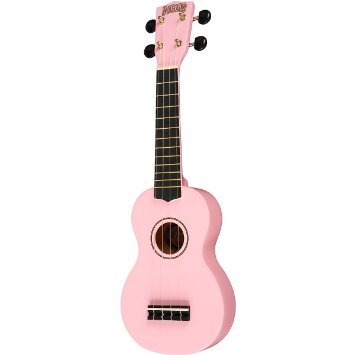
\includegraphics[width=5cm]{../img/ukulele.jpg}
\end{Slide}


% subjekt och predikat -> public static void: https://www.youtube.com/watch?v=1ZPaR_wH-R8


% \begin{Slide}{Koda i Scala}

%   {\footnotesize\it Melodi: McDonalds-låten}

% \begin{verbatim}

%           G         C             G          D
% Det finns stunder i livet som man alltid har kvar

%           G           C               D
% Det finns villkor och uttryck som man spar 

%         A           D             A           E
% Och där dörren står öppen finns gemenskap för fler 

% A      D      E       A
% Koda i Scala; det ger meeeeeeer! 
% \end{verbatim}

% \end{Slide}




\fi

%!TEX encoding = UTF-8 Unicode
%!TEX root = ../exercises.tex

\ifPreSolution

\Exercise{\ExeWeekTHIRTEEN}\label{exe:W13}
\begin{Goals}
\item Kunna skriva tentamenslika program med papper, penna och snabbreferens som enda hjälpmedel.
\item Förbereda projektredovisningen.
\item Kunna skapa dokumentation med \code{scaladoc} och \code{javadoc}.
\item Kunna skapa jar-filer.
\end{Goals}

% \begin{Preparations}
% \item \StudyTheory{13}
% \end{Preparations}

\else

\ExerciseSolution{\ExeWeekTHIRTEEN}

\fi


\subsection{Förberedelse inför examination}




\WHAT{Gör en extenta.} %%%%%%%%%%%%%%%%%%%%%%%%%%%%%%%%%%%%%%%%%%%%%%%%%%%%%%%%

\QUESTBEGIN

\Task \what~\TODO

\SOLUTION

\TaskSolved \what~\TODO

\QUESTEND




\WHAT{Förbered din projektredovisning.} %%%%%%%%%%%%%%%%%%%%%%%%%%%%%%%%%%%%%%%

\QUESTBEGIN

\Task \what~\TODO

\SOLUTION

\TaskSolved \what~\TODO

\QUESTEND



\WHAT{Skapa dokumentation.} %%%%%%%%%%%%%%%%%%%%%%%%%%%%%%%%%%%%%%%%%%%%%%%%%%%

\QUESTBEGIN

\Task  \what~

\Subtask \TODO kör nedan kommando i terminalen:

\begin{REPL}
> scaladoc paket.scala
> ls
> firefox index.html   # eller öppna index.html i valfri webbläsare
\end{REPL}

Vad händer?

\Subtask Lägg till några fler metoder i något av objekten i filen \code{paket.scala} och lägg även till några dokumentationskommentarer. Kompilera om och kör. Generera om dokumentationen.

\begin{verbatim}
//... ändra i filen paket.scala

/** min paketdokumentationskommentar p2 */
package p2 {
  /** min paketdokumentationskommentar p21 */
  package p21 {
    /** ett hälsningsobjekt */
    object hello {
      /** en hälsningsmetod i p2.p21 */
      def hello = println("Hej paket p2.p21!")

      /** en metod som skriver ut tiden */
      def date = println(new java.util.Date)
    }
  }
}

\end{verbatim}

\begin{REPL}
> gedit paket.scala
> scalac paket.scala
> jar cvf mittpaket.jar gurka
> scala -cp mittpaket.jar
scala> gurka.tomat.banan.p2.p21.hello.date
scala> :q
> scaladoc paket.scala
> firefox index.html
\end{REPL}

\SOLUTION


\TaskSolved \what

\SubtaskSolved  -

\SubtaskSolved  -

\QUESTEND



\WHAT{Repetera övningar och laborationer.} %%%%%%%%%%%%%%%%%%%%%%%%%%%%%%%%%%%%

\QUESTBEGIN

\Task \what~\TODO

\SOLUTION

\TaskSolved \what~\TODO

\QUESTEND

%!TEX encoding = UTF-8 Unicode

%!TEX root = ../compendium2.tex


\Assignment{life}

%\begin{Goals}
%    \item Kunna använda matriser som en datastruktur.
%    \item Kunna separera modell från vy med hjälp av \emph{Model-View}-uppdelning.
%    \item Känna till grundläggande cellulära automata. % \eng{cellular automata}.
%    % Följande rad är kanske inte aktuell, trådar tas upp i övningarna och hör inte riktigt hemma här då det är svårt att få in på ett smakligt sätt då Scala-kompilatorn och JVMen redan lyckas optimera koden så att den blir parallell.
%    %\item Känna till trådar, en grundläggande metod för att köra flera metoder \emph{samtidigt}.
%\end{Goals}
%
%
%\begin{Preparations}
%    \item Läs igenom laborationen.
%    \item Bekanta dig med kodskelettet.
%    \item Börja skriva konstruktorn för \code{ArrayMatrix2D} som handleds i uppgift 1a.
%    % TODO: The following are just "fun" preparations, which will give the student more insight into the field but aren't
%    %       actually required to complete the lab. They are optionals really.
%    %\item Läs om Life på Wikipedia.
%    %\item Läs om Cellulära automata på Wikipedia.
%\end{Preparations}

\subsection{Bakgrund}

% Hur mycket bakgrund, vilken typ av bakgrund är lämplig/intressant/relevant?
Spelet Life (även kallat \emph{Conway's Game of Life} efter skaparen och matematikern John Horton Conway) simulerar en koloni av encelliga organismer som lever, förökar sig och dör på ett rutnät (även kallat bräde). Varje enskild cells överlevnad beror på dess omgivning, vilket kan beskrivas med några enkla regler. Detta är gemensamt för alla cellulära automater. Spelet går ut på att simulera flera generationer av någon uppsättning celler, en såkallad cellkoloni, startkonfiguration eller frö (eng. \textit{seed}). Många sådana cellkolonier kan i Life verka bete sig `levande' och spelet har därifrån fått sitt namn.\footnote{Detta är ett exempel på s.k. `emergence' och `self-organization'} Spelet har inga medvetna spelare (ett så kallat `zero-player game') och om reglerna följs så kommer slutresultatet fullständigt bero på startkonfigurationen.

\vspace{5mm}

I denna laboration ska vi implementera en datastruktur för brädet samt reglerna för Life.

I extrauppgifterna kommer det även finnas möjlighet att utforska två andra exempel på cellulära automater.

\vspace{5mm}

För mer om Game of Life, se Wikipedia:

\begin{itemize}[noitemsep,topsep=0pt]
    	\item Engelska: \url{https://en.wikipedia.org/wiki/Conway's_Game_of_Life}
    	\item Svenska: \url{https://sv.wikipedia.org/wiki/Game_of_Life}
\end{itemize}


\subsection{Reglerna i Life}
\label{subsec:life-rules}

Varje cells tillstånd i nästa generation bestäms av följande regler:
\begin{enumerate}
    \item Om en levande cell har två eller tre grannar så lever den vidare.
    \item Om en levande cell har mindre än två eller mer än tre grannar dör den (av underpopulation respektive överpopulation).
    \item Om cellen är död och har exakt tre grannar så föds den och dess tillstånd ändras till levande, annars fortsätter den vara död.
\end{enumerate}

Med grannar menas i Life de s.k. Moore-grannarna. Dessa är helt enkelt de närmsta omgivande cellerna vertikalt, horizontalt och diagonalt.

\begin{figure}[h]
  \begin{center}
    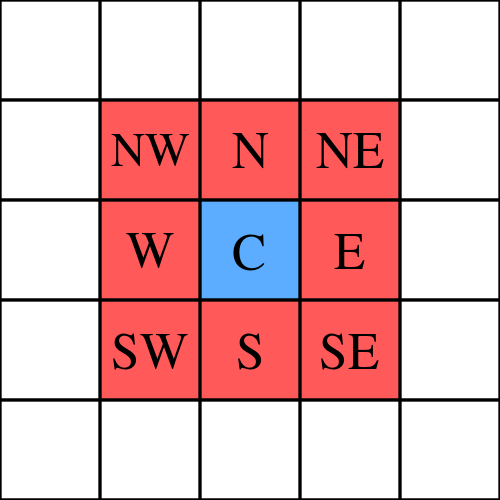
\includegraphics[width=0.5\textwidth]{../img/w12-lab/moore_neighborhood.png}
  \end{center}
  \caption{Moore-grannskapet består av nio celler: mittcellen samt de åtta omringande cellerna.\protect\footnotemark}
  \label{fig:threads:life:moore-neighborhood}
\end{figure}
\footnotetext{Källa: \url{https://commons.wikimedia.org/wiki/File:Moore_neighborhood_with_cardinal_directions.svg}}


\subsection{Beskrivning av Workspace}

I workspacet finner ni bl.a. paketen \code{models}, \code{rules} och \code{views}. I labben kommer ni främst ändra i \code{models}-paketet, men ni kommer även implementera reglerna för Life i \code{rules/LifeRule.scala}. Paketet \code{views} kommer med färdigimplementerad kod för två vyer \code{CellularConsoleView} samt \code{CellularGuiView}.

Utöver paketen finner ni i samma mapp några körbara Scala-filer som kan användas för att starta upp ett användargränssnitt som ritar upp brädet och låter användaren `spela' spelet. Den första av dessa filerna ni ska titta i och senare köra är \code{life.scala}.

Läs igenom de två filerna i \code{models}-paketet noga. Det är där ni kommer spendera den mesta av tiden.


\subsection{Obligatoriska uppgifter}
	% Förslag på hur de kan bygga upp programmet:
    % 1) skapa en main-klass som öppnar ett fönster som visar ett x gånger y stort fönster.
    % 2) [Kommer inte göras] skapa en klass Cell som har attributet levande eller död. Gör en metod där man kan ändra tillståndet på cellen.
    % 3) skapa en matris av celler som alla initieras som döda.
	% 4) koppla ihop modellen och vyn så att om man genom att klicka i vyn kan ändra cellens tillstånd. Testa att det fungerar. Gör så att vyn uppdateras efter cellerna i modellen när man klickar på "next generation".
	% 5) Studera traitet Rule i filen blahblah. Implementera reglerna (ge lite förklarande kodexempel för traitet Rule eller var det finns)
	% 6) Skriv metod(er) som räknar upp generationer.
	% 7) Testa nedanstående startfigurer (inkludera bilder på t ex en slider). Beter det sig som förväntat?


\Task Skapa en modell som kan visas i vyer som implementerar \code{CellularView2D}.

Spelbrädet består av en matris med $n$ rader och $m$ kolumner. ($n$ och $m$ brukar ibland modelleras som $\infty$, men vi kommer begränsa oss för enkelhetens skull).

Varje cell i matrisen kan vid varje tidpunkt (i varje generation) ha ett av två tillstånd: levande eller död. Dessa kommer vi för enkelhetens skull att representera som 1 eller 0, respektive. Detta för att göra det enklare att räkna ihop hur många levande grannar en cell har.

\Subtask Implementera konstruktorn i kompanjonsobjektet för \code{ArrayMatrix2D}.

För att skapa en matris ska vi använda oss av Scalas inbyggda datastruktur \code{Array}. Denna datastruktur har en användbar konstruktur \code{ofDim[T](n1: Int, n2: Int)} som vi ska använda för att skapa \emph{rows} stycken arrayer av storlek \emph{cols} inuti en annan array.

Ett exempel av resultatet från \code{Array.ofDim[Int](3, 3)} är följande ekvivalenta kod:

\begin{Code}
Array(
	Array(0,0,0),
	Array(0,0,0),
	Array(0,0,0)
)
\end{Code}

% Här nedan ser vi en sådan array utskriven i en komma-separerad lista. Detta är ett vanligt och enkelt dataformat som kallas CSV.\footnote{Förkortningen CSV står för Comma Separated Values}

%\begin{Code}
%0,0,0
%0,0,0
%0,0,0
%\end{Code}

\Subtask Implementera de övriga metoderna i \code{ArrayMatrix2D}. Läs igenom kommentarerna för de oimplementerade metoderna i traitet \code{Matrix2D} för kommentarer om vad som ska göras.


\Subtask Testa implementationen. Ta gärna hjälp av metoden \code{randomize} som finns på alla objekt som ärver traitet \code{Matrix2D}. Med den kan man enkelt slumpa fram nya tillstånd på brädet på följande vis:

\begin{Code}
// Slumpar varje cell i matrisen 'matrix' till antingen 0 eller 1
matrix.randomize(2)
\end{Code}

För att nu kontrollera att allt har blivit rätt kan vi visa upp matrisen i terminalen med hjälp av \code{CellularConsoleView}. Ett exempel på detta finns i \code{life_console.scala}.

\begin{Code}
// Skriver ut brädet i konsolen
CellularConsoleView.display(matrix)
\end{Code}

Men detta testar inte för alla möjliga fel, så för säkerhets skull kan vi även testa att placera ut en s.k. glider i brädet med hjälp av metoden \code{place} som finns implementerad i det ärvda traitet \code{Matrix2D}.

\begin{Code}
// Placerar ut en glider med sitt övre vänstra hörn i punkten
// (3, 1), d.v.s. på rad 4 och kolumn 2 (då vi noll-indexerar)
matrix.place(entities.glider, 3, 1)
\end{Code}

\begin{figure}[h]
  \begin{center}
    % Reflectbox here since glider in entities package is a reflection of the image.
    \reflectbox{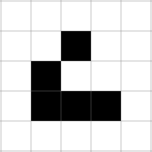
\includegraphics[width=0.3\textwidth]{../img/w12-lab/glider.png}}
  \end{center}
  \caption{En så kallad \textit{glider}. Vanligt förekommande varelse i Life.}
  \label{fig:threads:life:glider}
\end{figure}

Testa nu att rita ut brädet igen (utan \code{randomize} den här gången) för att se till att glidern hamnade rätt både med avseende på orientering och position. Den ska vara roterad precis som i figur \ref{fig:threads:life:glider}.


\Task Implementera Life-regeln med hjälp av traitet \code{Rule}.

Nu har vi vår datastruktur för brädet på plats, så det är dags att faktiskt implementera reglerna för Life. För att göra detta ska vi implementera objektet \code{LifeRule} som ärver traitet \code{Rule} vilket är ett interface som cellulära automaters regler kan implementera. Men först ska vi implementera några hjälpsamma funktioner, så att vår kod i \code{LifeRule} senare blir mer lättläst.

\Subtask Implementera \code{mooreNeighborsPositions} samt \code{mooreNeighborsStates} i \code{Matrix2D}.

Då Life-regeln förlitar sig på Moore-grannskapet som tidigare nämnts så behöver vi ett smidigt sätt att få ut grannarna för en viss cell. Detta är vad funktionerna \code{mooreNeighborsPositions} samt \code{mooreNeighborsStates} ska göra.

När \code{mooreNeighborsStates} implementeras är det viktigt att ta hänsyn till om grannarna faktiskt finns (då vårt bräde är av begränsad storlek).
För detta bör man använda \code{isWithinMatrix}-metoden som tidigare implementerades i \code{ArrayMatrix2D}.

Börja med att implementera \code{mooreNeighborsPositions} och använd sedan den för att implementera \code{mooreNeighborsStates}.

\Subtask Implementera \code{apply} i ett nytt objekt \code{LifeRule} som implementerar \code{Rule}.

Nedan finns specifikationen för traitet \code{Rule}. Den innehåller endast en metod \code{apply} vars uppgift är att ta ett bräde samt en position på brädet och returnera vad denna position ska innehålla för värde i nästa generation.

\begin{ScalaSpec}{Rule}
// apply tar en matris samt en position i matrisen (row, col)
// och applicerar regeln på den positionen
def apply(m: ArrayMatrix2D, row: Int, col: Int): Int
\end{ScalaSpec}

Reglerna för Life finner ni ovan i avsnitt \ref{subsec:life-rules}.

\Subtask Testa implementationen.

För att nu i praktiken applicera vår regel på brädet ska vi använda oss av metoden \code{applyRule} som finns i \code{ArrayMatrix2D}.

Om man har problem med att sin regel inte beter sig som förväntat kan man felsöka genom att returnera antalet grannar istället för cellens levande/död-tillstånd. Efter att ha applicerat hela s.k. \code{NeighborsRule} kan man visa upp resultatet med \code{CellularConsoleView} för att se om programmet räknar grannar korrekt.


\Task Skapa en ny modell som ''wrappar'' i kanterna.

Just nu har vi ett udda beteende i modellen, nämligen att alla celler utanför brädet i praktiken räknas som döda. För att få ett lite mer intressant beteende vill vi nu göra så att om exempelvis en glider åker in i höger vägg ska den komma ut ur vänster vägg. Detta kan göras med några små modifikationer till \code{ArrayMatrix2D}.

\Subtask Ändra metoden \code{isWithinMatrix} så att alla positioner är giltiga.

Då funktionen \code{mooreNeighborsStates} i \code{Matrix2D} använder sig av funktionen \code{isWithinMatrix} för att avgöra om celler är inom brädet måste vi se till att \code{isWithinMatrix} inte hindrar grann-funktionen från att hämta celler ''utanför'' brädet. Detta kan vi enkelt göra genom att kommentera ut hela den tidigare koden och istället alltid returnera \code{true}. Om vi nu försöker köra programmet kommer vi få \code{ArrayIndexOutOfBoundsException} eftersom vi ännu inte gjort så att hämtningar eller tilldelningar ''utanför'' brädet wrappar, vilket vi nu ska göra.

\Subtask Ändra metoderna \code{get} samt \code{set} så att hämtningar respektive tilldelningar utanför brädet wrappar.

För att åstadkomma wrappning måste vi göra så att alla hämtningar och tilldelningar utanför brädet ''går runt''. Detta kan enklast göras med hjälp av modulo-operatorn.

\begin{Code}
val wrapped_row = row % rows
\end{Code}

Men denna lösning tar inte hänsyn till negativa tal, vilket kan uppkomma när man t.ex. försöker hämta grannarna för cellen i det övre vänstra hörnet på brädet, d.v.s. position (0, 0). För att enkelt lösa detta kan man förskjuta hela \code{row} med \code{rows} så att man istället får följande:

\begin{Code}
val wrapped_row = (rows + row) % rows
\end{Code}

Vi kan använda oss av denna kunskap för att i metoderna \code{get} samt \code{set} se till att operationerna wrappar. Testa sedan din implementation genom att låta en glider glida in i en vägg.


\subsection{Frivilliga extrauppgifter}

Inom cellulära automata finns det många intressanta ting att utforska. Nedan finns några extrauppgifter som nyfikna och intresserade läsare uppmanas implementera då resultaten kan vara djupt tillfredställande. De kan göras i valfri ordning.


\Task Implementera spara och ladda.

När man leker runt med cellulära automater vill man ofta spara sina bräden så att man senare enkelt kan ladda in dem igen. För att göra detta ska vi i denna extrauppgift definiera ett dataformat som ska innehålla all data som behövs för att återskapa vår \code{ArrayMatrix2D}.

\Subtask Spara brädets tillstånd.

Tillståndet ska sparas till ett format som både är lätt att spara/exportera och ladda/importera. Det vi behöver spara är följande:

\begin{itemize}
	\item Brädets storlek, d.v.s. antalet rader och kolumner
	\item Hur många olika värden en cell på brädet kan anta
	\item Matrisen i sig, d.v.s. alla cellers värden
\end{itemize}

Det är metoden \code{ArrayMatrix2D.toFileFormat} som ska implementeras.

Vi föreslår att ni börjar filen med en rad innehållande de två värdena i punkt ett, samt värdet i punkt två. Separera dem med mellanslag, komma, eller en emoji (på egen risk). Därefter är det lämpligt att skriva ut matrisen rad för rad där varje cell skrivs ut som en etta eller nolla. Man kan göra detta utan separator för bräden där celler bara antar värden i intervallet 0-9, men det fungerar inte längre om en cell kan anta andra värden (såsom i uppgiften med cykliska cellulära automater nedan) då man inte längre kan lita på att en cell motsvaras av en enda siffra. För att lösa denna begränsning kan man separera sina värden med något tecken precis som för första raden.

Testa att spara genom att gå in i menyn i användargränssnittet och välja ''Save...''. Öppna den sparade filen med en texteditor för att verifiera att innehållet ser korrekt ut.

\Subtask Ladda in det sparade tillståndet.

Implementera metoden \code{ArrayMatrix2D.fromFileFormat} för att läsa in det sparade tillståndet.

Testa sedan att ladda genom att gå in i menyn i användargränssnittet och välja ''Load...''. Brädet ska nu se ut precis som det gjorde när det sparades.

\Task Implementera andra regler för cellulära automata.

Det finns massor med regler för cellulära automata med sina egna intressanta beteenden och tillstånd.
Gör den eller de du tycker verkar mest intressant!

Fler regler finns här: \url{https://en.wikipedia.org/wiki/Category:Cellular_automaton_rules}

Nedan följer några roliga exempel som valts ut och anses lämpliga.

\Subtask Implementera regeln för cykliska cellulära automater.

Denna typ av automata kallas cyklisk just för att det finns $N$ möjliga tillstånd och när tillståndet $N-1$ nås så är ''nästa'' tillstånd $0$.
Detta beteende kan beskrivas med modulo-operatorn: $T_{nästa} = (T_{nuvarande} + 1)\ \%\ N$

Regeln är att om en granne till den aktuella cellen har tillståndet exakt ett över cellens tillstånd så får cellen sin grannes tillstånd. Det vill säga om en granne har tillståndet $T_{nästa}$ så får även cellen i mitten det värdet.

För att få intressant beteende brukar man initialisera hela brädet så att varje cell får ett slumpvalt tillstånd.

En bra förberedelse för att implementera denna cellulära automat är att läsa Wikipedia-artikeln: \url{https://en.wikipedia.org/wiki/Cyclic_cellular_automaton}

    \Subtask{Implementera regeln för Wireworld.}

Wireworld skiljer sig från andra cellulära automata då man i Wireworld designar `kretsar' inte helt olika de som finns i moderna datorer.
På grund av detta är majoriteten av celler vanligtvis fast i ett dött tillstånd (isolatorer).

I Wireworld kan man skapa komponenter såsom dioder och transistorer. Med dessa kan man bygga logiska grindar och därmed hela datorer (som dock blir väldigt långsamma i jämförelse med datorerna de körs på).

En bra förberedelse för att implementera Wireworld är att läsa Wikipedia-artikeln: \url{https://en.wikipedia.org/wiki/Wireworld}

\begin{figure}[h]
    \begin{center}
        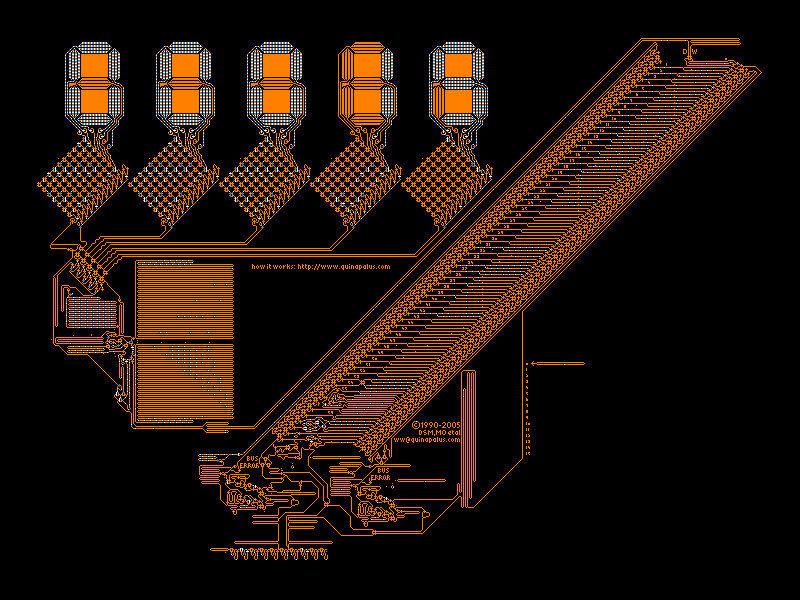
\includegraphics[width=0.8\textwidth]{../img/w12-lab/wireworld_computer.png}
    \end{center}
    \caption{En enkel dator implementerad i Wireworld.\protect\footnotemark}
    \label{fig:threads:life:wireworld-computer}
\end{figure}
\footnotetext{Källa: \url{http://www.quinapalus.com/wi-index.html}}


\subsection{Extra läsning}

\begin{itemize}

\item[] \textbf{Intressanta mönster i Life}

\begin{itemize}[noitemsep,topsep=0pt]
    \item \url{https://en.wikipedia.org/wiki/Spacefiller}
    \item \url{https://en.wikipedia.org/wiki/Spaceship_(cellular_automaton)}
\end{itemize}

\item[] \textbf{Intressanta automater}

\begin{itemize}[noitemsep,topsep=0pt]
	\item \url{https://en.wikipedia.org/wiki/Codd's_cellular_automaton}
	\item \url{https://en.wikipedia.org/wiki/Von_Neumann_universal_constructor}
\end{itemize}

\item[] \textbf{Intressanta resurser}

\begin{itemize}[noitemsep,topsep=0pt]
    \item Eric Weisstein's Treasure Trove of the Life Cellular Automaton: \\ \url{http://www.ericweisstein.com/encyclopedias/life/topics/}
\end{itemize}

\end{itemize}


% Kanske för nästa år
%\Task{Alternativ vy: Kör programmet i webbläsaren med Scala.js}


% Detta kan kräva speciell IDE (android-studio) och eventuellt en Android-emulator som inte kan köras på skolans datorer.
%\Task{Alternativ vy: Kör programmet på Android}


% Detta kommer antagligen inte ske då det lägger till signifikant komplexitet
% En bättre extrauppgift är att representera brädet som ett quadtree då det leder en in på Hashlife
%\Task{Implementera brädet som en sparse-matris}

%I den tidigare lösningen har vi allokerat en hel matris där bara en del av brädet vanligtvis är levande, en sådan matris kallas för en sparse matris (en matris där majoriteten av värdena är 0).
%    \Subtask{???}


%\Task{Implementera den supersnabba Hashlife}
%    Detta är en utmaning som kräver en viss kunskap om algoritmer och hashning som läsare av denna labben inte ännu förväntas inneha.
%    Den verkligt intresserade läsaren kan dock se denna uppgift som ett långtids-läromål och återkomma till uppgiften senare i sin utbildning när
%    hen känner sig redo.
%
%    En utförlig beskrivning om hashlife och quadtrees finnes på Wikipedia:
%    \begin{enumerate}
%        \item https://en.wikipedia.org/wiki/Hashlife
%        \item https://en.wikipedia.org/wiki/Quadtree
%    \end{enumerate}
%
%    \Subtask{Implementera QuadtreeMatrix2D}
%        Hashlife använder sig inte av en matris-representation för brädet utan använder sig istället av en datastruktur som heter Quadtrees.
%        Dessa fungerar som vanliga träd fast varje nod kan antingen ha exakt 4 brancher eller vara ett löv. Varje branchning delar upp en kvadrat
%        i 4 mindre kvadrater och varje löv representerar värdet för en kvadrat.
%
%        Quadtrees möjliggör att man kan beräkna tomma områden på brädet på konstant tid då man vet att ett helt område kommer förbli opåverkat utan
%        att behöva titta igenom varje cell.
%
%        \begin{figure}[h]
%            \begin{center}
%                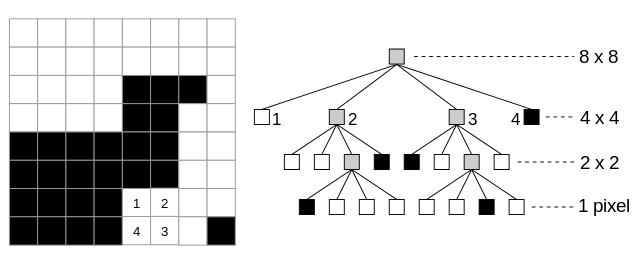
\includegraphics[width=0.7\textwidth]{../img/w12-lab/quadtree_bitmap.png}
%            \end{center}
%            \caption{Ett exempel på hur ett Quadtree använts för att representera en bitmap likt den som återfinns i Life}
%            % Källa: Wikipedia (https://commons.wikimedia.org/wiki/File:Quad_tree_bitmap.svg)
%        \end{figure}
%
%    \Subtask{Implementera hashlife}
%
%        Här kan vi inte handleda er, då det anses vara allt för långt utanför kursmålen. Men för den ambitiösa studenten refererar vi glatt till Wikipedia och önskar er lycka till!

%!TEX encoding = UTF-8 Unicode
%!TEX root = ../compendium2.tex

\Assignment{bank}

\subsection{Fokus}
\begin{itemize}[nosep,label={$\square$},leftmargin=*]
\item Kunna implementera ett helt program efter given specifikation
\item Kunna sätta samman olika delar från olika moduler
\item Förstå hur Java-klasser kan användas i Scala
\item Förstå och bedöma när immutable/mutable såväl som var/val bör användas i större sammanhang
\item Kunna använda sig av kompanjonsobjekt
\item Kunna läsa och skriva till fil
\item Kunna söka i olika datastrukturer på olika sätt
\end{itemize}

\subsection{Bakgrund}

I detta projekt ska du skriva ett program som håller reda på bankkonton och kunder i en bank. Programmet ska utöver att hålla reda på bankens nuvarande tillstånd även föra historik över alla tillståndsändringar. Historiken ska vara så pass detaljerad att det nuvarande tillståndet kan återskapas genom att återuppspela alla ändringar som finns lagrade i historiken.

Programmet ska vara helt textbaserat, man ska alltså interagera med programmet via terminalen där en meny skrivs ut och input görs via tangentbordet.

Du ska skriva större delen av programmet själv, utan någon färdig kod. Programmet ska dock följa de specifikationer som ges i uppgiften, såväl som de objektorienterade principer du lärt dig i kursen.

\subsection{Krav}

Kraven för bankapplikationen återfinns här nedan. För att bli godkänd på denna uppgift måste samtliga krav uppfyllas:

\begin{itemize}
\item Programmet ska ha följande menyval:

\begin{itemize}
\item 1. Hitta konton för en viss kontoinnehavare med angivet ID.
\item 2. Söka efter kunder på (del av) namn.
\item 3. Sätta in pengar på ett konto.
\item 4. Ta ut pengar på ett konto.
\item 5. Överföra pengar mellan två olika konton.
\item 6. Skapa ett nytt konto.
\item 7. Ta bort ett befintligt konto.
\item 8. Skriv ut bankens alla konton, sorterade i bokstavsordning efter innehavare.
\item 9. Återställa banken till tillståndet den hade vid ett givet datum. För enkelhetens skull får du permanent kassera all historik som skapades efter det datum banken återställs till.
\item 10. Avsluta.
\end{itemize}

\item När något av följande sker ska programmet notera det i historiken:
\begin{itemize}
\item Pengar sätts in på ett konto.
\item Pengar tas ut från ett konto.
\item Pengar överförs mellan två konton.
\item Ett konto skapas.
\item Ett konto tas bort.
\end{itemize}
\item Historiken ska sparas både i minnet och i en fil.
\item Då programmet startas ska det läsa in historikfilen för att återskapa tillståndet som banken hade tidigare.
\item Allt som berör användargränssnittet (såsom utskrifter till terminalen och inläsning från terminalen) ska ske i \code{BankApplication} eller hjälpklasser till \code{BankApplication}, inte i någon annan av klasserna som specificeras i uppgiften.
\item Alla metoder och attribut ska ha lämpliga åtkomsträttigheter.
\item Valen av val/var och immutable/mutable måste vara lämpliga.
\item Din indata måste ge samma resultat som i exemplen i bilagan.
\item Rimlig felhantering ska finnas. Det är alltså önskvärt att programmet inte kraschar då man matar in felaktig input, utan istället säger till användaren att input är ogiltlig.
\item Programdesignen ska följa de specifikationer som är angivna nedan.
\item Det räcker med att banken ska kunna hantera heltal, men detta ska göras med klassen \code{BigInt}.
\item Klassen \code{BankAccount} ska generera ett unikt kontonummer för varje konto. Dessa ska återställas om bankens tillstånd återställs till ett tidigare datum, d.v.s. att om en återställning av banken tar bort ett konto så ska dess kontonummer återigen bli tillgängligt.
\end{itemize}

\subsection{Design}
Nedan följer specifikationerna för de olika klasserna bankapplikationen måste innehålla:

\begin{ScalaSpec}{Customer}
/**
 * Describes a customer of a bank with provided name and id.
 */
case class Customer(name: String, id: Long) = {
	override def toString(): String = ???
}
\end{ScalaSpec}


\begin{ScalaSpec}{BankAccount}
/**
 * Creates a new bank account for the customer provided.
 * The account is given a unique account number and initially
 * has a balance of 0 kr.
 */
class BankAccount(val holder: Customer) = {

  /**
   * Deposits the provided amount in this account.
   */
  def deposit(amount: Int): Unit = ???

  /**
   * Returns the balance of this account.
   */
  def getBalance: Int = ???

  /**
   * Withdraws the provided amount from this account,
   * if there is enough money in the account. Returns true
   * if the transaction was successful, otherwise false.
   */
  def withdraw(amount: Int): Boolean = ???
}
\end{ScalaSpec}


\begin{ScalaSpec}{Bank}
/**
 * Creates a new bank with no accounts and no history.
 */
class Bank() = {

 /**
   * Returns a list of every bank account in the bank.
   * The returned list is sorted in alphabetical order based
   * on customer name.
   */
  def getAllAccounts(): Vector[BankAccount] = ???

  /**
   * Returns the account holding the provided account number.
   */
  def findByNumber(accountNbr: Int): Optional[BankAccount] = ???

  /**
   * Returns a list of every account belonging to
   * the customer with the provided id.
   */
  def findAccountsForHolder(id: Long): Vector[BankAccount] = ???

  /**
   * Returns a list of all customers whose names match
   * the provided name pattern.
   */
  def findByName(namePattern: String): Vector[Customer] = ???

 /**
   * Executes an event in the bank.
   * Returns a string describing whether the
   * event was successful or failed.
   */
  def doEvent(event: BankEvent): String = ???

  /**
   * Resets the bank to the state it had at the provided date.
   * Returns a string describing whether the event was
   * successful or failed.
   */
  def returnToState(returnDate: Date): String = ???
}
\end{ScalaSpec}


Till din hjälp innehåller kursens workspace följande färdigskrivna klasser:
\begin{itemize}
\item \code{Date}, en enkel wrapper av \code{Java.time} som du ska använda för att representera tidsstämplar.
\item \code{BankEvent} med tillhörande subtyper, som du ska använda för att representera förändringar av bankens tillstånd.
\end{itemize}


\subsection{Tips}

\begin{itemize}
\item Det enda sättet att förändra tillståndet för en \code{Bank} ska vara (förutom att anropa \code{returnToState}) att anropa \code{doEvent} med en \code{BankEvent} som beskriver tillståndsförändringen. Vid en första anblick kan detta kan verka lite väl bökigt, men när ändringshistoriken ska implementeras kommer det vara till stor hjälp att det finns en \code{BankEvent} som representerar varje ändring.

\item För att skriva till fil på ett enkelt sätt kan man t.ex. använda sig av statiska metoder i klassen \code{Files} som finns tillgänglig i \code{java.nio.file}. För att undvika portabilitetsproblem kan man då använda sig av ett bestämt \code{Charset}, t.ex. \code{UTF_8}, som finns tillgänglig i \code{java.nio.charset.StandardCharsets.UTF_8}.

\item För att läsa ifrån en fil kan man t.ex. använda sig av \code{Source} som finns tillgänglig i \code{scala.io.Source}.

\item Var noggrann med att testerna klarar alla tänkbara fall, och tänk på att fler fall än dem som givits i exempel kan förekomma vid rättning.
\end{itemize}

\subsection{Obligatoriska uppgifter}

\Task Implementera klassen \code{Customer}.

\Task Implementera klassen \code{BankAccount}.

\Task Skapa singelobjektet \code{BankApplication}, som ska innehålla \code{main}-metoden. Det kan vara bra att innan man fortsätter se till att denna skriver ut menyn korrekt och kan ta input från tangentbordet som motsvarar de menyval som finns.

\Task Implementera klassen \code{Bank}.

\Subtask Implementera menyval 6 och 8. Testa noga.

\Subtask Implementera ändringshistoriken. Varje gång \code{doEvent} anropas ska dess \code{BankEvent}-argument läggas till i historiken tillsammans med det nuvarande datumet.

\Subtask Implementera alla andra menyval, förutom menyval 9. Testa de nya menyvalen noga efterhand som du implementerar dem, i synnerhet så att ändringshistoriken fungerar korrekt. Gör de utökningar du anser behövs.

\Task Implementera säkerhetskopiering av historiken.

\Subtask När en \code{BankEvent} läggs till i historiken ska den också skrivas till en historikfil omedelbart. Banken ska ej behöva avslutas för att utskriften ska hamna på fil, om så vore fallet kan information gå förlorad om banken kraschar.

I workspace-katalogen för denna projektuppgift finns en historikfil bifogad. För bekvämlighet finns ett utdrag av denna fil infogad nedanför. Inläsning och utskrift ska ske med dess format:\\~\\
2016 3 7 10 6 N 850127 Fredrik\newline
2016 3 7 10 28 D 1000 16500\newline
2016 3 9 10 52 W 1000 3900\newline
2016 3 9 11 8 N 900318 Casper\newline
2016 3 9 16 28 D 1001 6500\newline
2016 4 1 10 11 W 1001 1900\newline
2016 4 1 11 19 W 1001 2000\newline
2016 4 2 16 33 N 651002 Björn\newline
2016 4 2 16 46 D 1002 25000\newline
2016 4 3 10 11 T 1002 1000 4000\\~\\
Formen är alltså:\\~\\
\textbf{År  Månad  Dag  Timme  Minut  BankEventTag  Parametrar}
\\~\\
De olika klasserna av \code{BankEvent} representeras med följande bokstav:

\begin{itemize}
\item D - \code{Deposit}
\item W - \code{Withdraw}
\item T - \code{Transfer}
\item N - \code{NewAccount}
\item E - \code{DeleteAccount}
\end{itemize}

\Subtask När programmet startar ska det läsa in alla händelser från historikfilen och återuppspela dem en efter en. På så sätt kan bankens tillstånd återställas, fastän vi bara har sparat ändringshistoriken och inte själva tillståndet.

\Task Implementera menyval 9 genom att först nollställa bankens tillstånd och sedan återuppspela allt i historiken som hände före det givna datumet. Resten av historiken bör tas bort permanent, både i minnet och i historikfilen.


\subsection{Frivilliga extrauppgifter}

Gör först klart projektets obligatoriska delar. Därefter kan du, om du vill, utöka ditt program enligt följande.

\Task Skriv en eller flera av klasserna \code{Customer} och \code{BankAccount} i Java istället och använd dig av dessa i din Scala-kod.

\Task	Implementera ett nytt menyalternativ som skriver ut all kontohistorik för en given person. I historiken ska finnas typ av händelse med tillhörande parametrar, dåvarande saldo vid händelsen, såväl som datumet för händelsen.

\subsection{Exempel på körning av programmet}

Nedan visas möjliga exempel på körning av programmet. Data som matas in av användaren är markerad i fetstil.
Ditt program måste inte se identiskt ut, men den övergripande strukturen såväl som resultat av körningen ska vara densamma.
När det första exemplet börjar förutsätts det att banken inte har några konton.

Listan över val, som är markerad i kursiv stil i det första exemplet, är inte utskriven i senare exempel för att spara plats på pappret. Ditt program ska alltid skriva ut listan över val före användaren ska mata in ett val.

% This environment uses minipage to prevent column breaks from occurring in the middle of an example
\newenvironment{exampleblock}
	{\begin{minipage}{\columnwidth}
	 - - - - - - - - - - - - - - - - - - - - - - - - - - -\\}
	{\end{minipage}}

\begin{multicols}{2}
\noindent
\begin{exampleblock}
\textit{
1.   Hitta ett konto för en given kund\\
2.   Sök efter kunder på (del av) namn\\
3.   Sätt in pengar\\
4.   Ta ut pengar\\
5.   Överför pengar mellan konton\\
6.   Skapa nytt konto\\
7.   Radera existerande konto\\
8.   Skriv ut alla konton i banken\\
9.   Återställ banken till ett tidigare datum\\
10.  Avsluta\\
}
Val: \textbf{6}\\
Namn: \textbf{Adam Asson}\\
Id: \textbf{6707071234}\\
Nytt konto skapat med kontonummer: 1000\\
10:03:0 CET 14 / 5 - 2016\\
\end{exampleblock}
\begin{exampleblock}
Val: \textbf{1}\\
Id: \textbf{6707071234}\\
Konto 1000 (Adam Asson, id 6707071234) 0 kr\\
10:04:0 CET 14 / 5 - 2016\\
\end{exampleblock}
\begin{exampleblock}
Val: \textbf{6}\\
Namn: \textbf{Berit Besson}\\
Id: \textbf{8505255678}\\
Nytt konto skapat med kontonummer: 1001\\
10:12:0 CET 14 / 5 - 2016\\
\end{exampleblock}
\begin{exampleblock}
Val: \textbf{2}\\
Namn: \textbf{adam}\\
Adam Asson, id 6707071234\\
10:15:0 CET 14 / 5 - 2016\\
\end{exampleblock}
\begin{exampleblock}
Val: \textbf{8}\\
Konto 1000 (Adam Asson, id 6707071234) 0 kr\\
Konto 1001 (Berit Besson, id 8505255678) 0 kr\\
10:13:0 CET 14 / 5 - 2016\\
\end{exampleblock}
\begin{exampleblock}
Val: \textbf{6}\\
Namn: \textbf{Berit Besson}\\
Id: \textbf{8505255678}\\
Nytt konto skapat med kontonummer: 1002\\
13:56:0 CET 14 / 5 - 2016\\
\end{exampleblock}
\begin{exampleblock}
Val: \textbf{2}\\
Namn: \textbf{erit}\\
Berit Besson, id 8505255678\\
14:01:0 CET 14 / 5 - 2016\\
\end{exampleblock}
\begin{exampleblock}
Val: \textbf{3}\\
Kontonummer: \textbf{1000}\\
Summa: \textbf{5000}\\
Transaktionen lyckades.\\
14:36:0 CET 14 / 5 - 2016\\
\end{exampleblock}
\begin{exampleblock}
Val: \textbf{5}\\
Kontonummer att överföra ifrån: \textbf{1000}\\
Kontonummer att överföra till: \textbf{1001}\\
Summa: \textbf{1000}\\
Transaktionen lyckades.\\
14:37:0 CET 14 / 5 - 2016\\
\end{exampleblock}
\begin{exampleblock}
Val: \textbf{8}\\
Konto 1000 (Adam Asson, id 6707071234) 4000 kr\\
Konto 1001 (Berit Besson, id 8505255678) 1000 kr\\
Konto 1002 (Berit Besson, id 8505255678) 0 kr\\
14:52:0 CET 14 / 5 - 2016\\
\end{exampleblock}
\begin{exampleblock}
Val: \textbf{7}\\
Ange konto att radera: \textbf{1002}\\
Transaktionen lyckades.\\
14:01:0 CET 14 / 5 - 2016\\
\end{exampleblock}
\begin{exampleblock}
Val: \textbf{8}\\
Konto 1000 (Adam Asson, id 6707071234) 4000 kr\\
Konto 1001 (Berit Besson, id 8505255678) 1000 kr\\
14:01:0 CET 14 / 5 - 2016\\
\end{exampleblock}
\begin{exampleblock}
Val: \textbf{9}\\
Vilket datum vill du återställa banken till?\\
År: \textbf{2016}\\
Månad: \textbf{5}\\
Datum (dag): \textbf{9}\\
Timme: \textbf{18}\\
Minut: \textbf{10}\\
Banken återställd.\\
15:00:0 CET 14 / 5 - 2016\\
\end{exampleblock}
\begin{exampleblock}
Val: \textbf{8}\\
Konto 1002 (Björn, id 651002) 25900 kr\\
Konto 1001 (Casper, id 900318) 4600 kr\\
Konto 1003 (Eva, id 950908) 6300 kr\\
Konto 1000 (Fredrik, id 850127) 11800 kr\\
Konto 1004 (Kajsa, id 810722) 17000 kr\\
15:01:0 CET 14 / 5 - 2016\\
\end{exampleblock}
\begin{exampleblock}
Val: \textbf{3}\\
Kontonummer: \textbf{1005}\\
Summa: \textbf{5000}\\
Transaktionen misslyckades. Inget sådant konto hittades.\\
15:06:0 CET 14 / 5 - 2016\\
\end{exampleblock}

\end{multicols}

%!TEX encoding = UTF-8 Unicode
%!TEX root = ../compendium.tex

\Assignment{tictactoe}

\subsection{Obligatoriska uppgifter}

\Task En uppgift.

\Subtask En underuppgift.

\Subtask En underuppgift.

\subsection{Frivilliga extrauppgifter}

\Task En uppgift.

\Subtask En underuppgift.

\Subtask En underuppgift.
%!TEX encoding = UTF-8 Unicode
%!TEX root = ../compendium.tex

\Assignment{imageprocessing}

\subsection{Bakgrund}

En digital bild består av ett rutnät (en matris) av pixlar. Varje pixel har en färg, och om man har många pixlar flyter de samman för ögat så att de tillsammans skapar en bild.

Det finns olika system för hur man färgsätter de olika pixlarna. T.ex. så används CMYK-systemet (cyan, magenta, gul, svart) vid blandning av färg som ska tryckas på papper eller annat material. På en dator däremot används vanligtvis RGB-systemet. RGB-systemet har tre grundfärger: röd, grön och blå. Mättnaden av varje grundfärg anges av ett heltal som vi i fortsättningen förutsätter ligger i intervallet [0, 255]. 0 anger ”ingen färg” och 255 anger ”maximal färg”. Man kan därmed representera 256 × 256 × 256 = 16 777 216 olika färgnyanser. Man kan också representera gråskalor; det gör man med färger som har samma värde på alla tre grundfärgerna: (0, 0, 0) är helt svart, (255, 255, 255) är helt vitt.


\subsection{Uppgiften}
Du ska skriva ett program där du implementerar olika filter som ska manipulera en given bild på ett flertal olika sätt. Filterklasserna ska ärva från en abstrakt \code{ImageFilter}-klass som är skriven i Java. \code{ImageFilter}-klassen hittar du i cslib.

Följande beskriver \code{ImageFilter}-klassen.

\begin{JavaSpec}{abstract class ImageFilter}
/**
 * Skapar ett filterobjekt med ett givet namn.
 */
protected ImageFilter(String name);

/**
 * Tar reda på filtrets namn.
 */
public String getName();

/**
 * Filtrerar bilden i matrisen inPixels och returnerar
 * resultatet i en ny matris. Utnyttjar eventuellt 
 * värdet av paramValue
 */
public abstract Color[][] apply(Color[][] inPixels,
				 double paramValue);

/**
 * Berättar huruvida ett filter behöver ett parmetervärde eller inte
 * @return true ifall parametervärde behövs, annars false
 */
public abstract boolean needsParameter();

/**
 * Beräknar intensiteten hos alla pixlarna i pixels,
 * returnerar resultatet i en ny matris.
 */
protected short[][] computeIntensity(Color[][] pixels):

/**
 * Faltar punkten p[i][j] med faltningskärnan kernel.
 * 
 * @param p 		matris med talvärden
 * @param i 		radindex får den aktuella punkten
 * @param j 		kolonnindex får den aktuella punkten
 * @param kernel	faltningskärnan, en 3x3-matris
 * @param weight	summan av elementen i kernel
 * @return 		resultatet av faltningen
 */
protected short convolve(short[][] p, int i, int j, 
			short[][] kernel, int weight);
\end{JavaSpec}

Utöver filterklasserna ska du även skapa ett program där du kan välja ett variabelt antal filter och sedan applicera dessa på en bild. För att åstadkomma detta ska du implementera klasserna \code{FilterChooser}, som hanterar val av filter, och \code{FilterList} som representerar vilka filter som ska användas. Klasserna har följande specifikationer:

\begin{ScalaSpec}{FilterList}
class FilterList = ???

/** Adds a filter to the FilterList */
def addFilter(filter: ImageFilter): Unit = ???
  
/** Applies all the filters on the given Image and draws it in SimpleWindow */
def applyFilters(image: Image, sw: SimpleWindow): Unit = ???
\end{ScalaSpec}

\begin{ScalaSpec}{FilterChooser}
/** Creates a FilterChooser with all the available filters */
class FilterChooser(filters: Array[ImageFilter]) = ???
  
/** Shows which filters are available and lets the user choose filters
*   until an escape sequence has been given and returns a FilterList which
*   contain the chosen filters
*   Example: 
*   Tryck på 1 för Blått-filter
*   Tryck på 2 för Kontrast-filter
*   Tryck på 3 för Gauss-filter
*   Tryck på 4 för Sobel-filter
*   Tryck 42 om du inte vill ha fler filter
*/
def chooseFilters(): FilterList = ???
\end{ScalaSpec}

Till din hjälp får du en \code{Image}-klass som representerar en bild samt ett \code{ImageUI} som hjälper dig att ladda in en JPEG bild.

\begin{ScalaSpec}{Image}
class Image(val image: BufferedImage);

/** Returns a matrix of Color-objects that represents an image */
def getColorMatrix: Array[Array[Color]];

/** Updates the image in accordance with the given Color-matrix */
def updateImage(pixels: Array[Array[Color]]): Unit;
\end{ScalaSpec}


\Task \textbf{Blåfilter.} Skriv en klass \code{BlueFilter} som skapar en blå version av bilden. Det vill säga skapa ett filter där varje pixel bara innehåller den blå komponenten. Testa filtret genom att skapa ett \code{ImageProcessing}-object som ska innehålla en \code{main}-metod (\code{ImageProcessing} ska användas och utökas i senare uppgifter). Använd \code{ImageUI} för att välja en bild på följande sätt:
\begin{Code}
val im = new Image(ImageUI.getImage)
\end{Code}
Använd \code{SimpleWindow} samt \code{image} attributet från \code{Image}-objektet för att visa bilden. 

\Task \textbf{inverteringsfilter.} Skriv en klass \code{InvertFilter} som inverterar en bild dvs skapar en ''negativ'' kopia av bilden. Ljusa färger ska alltså bli mörka och mörka färger ska bli ljusa.
Fundera över vad som kan menas med en inverterad eller negativ kopia: de nya RGB-värdena är inte ett dividerat med de gamla värdena (då skulle de nya värdena kunna bli flyttal) och inte de gamla värdena med ombytt tecken (då skulle de nya värdena bli negativa).

\Task \textbf{Gråskalningsfilter.} Skriv en klass \code{GrayScaleFilter} som gör om bilden till en gråskalebild. Använd \code{ImageFilter}s \code{computeIntensity} metod för att bestämma vilken intensitet varje pixel ska ha. Om intensiteten i en pixel till exempel är 105 så ska ett nytt \code{Color}-objekt med värdena (105, 105, 105) skapas.

\Task \textbf{Krypteringsfilter.} Skriv en klass \code{XORCryptFilter} som krypterar bilden med xor-operatorn ˆ. Denna operator gör binär xor mellan bitarna i ett heltal. Exempelvis ger 8 ˆ 127 värdet 119. Om man gör xor igen med 127, alltså 119 ˆ 127, får man tillbaka värdet 8. Varje pixel krypteras genom att använda xor-operatorn med ursprungsvärdena för rött, grönt och blått tillsammans med ett slumpmässigt heltalsvärde som genereras av Scalas Random klass. Använd \code{paramValue} för att ge \code{Random}-objektet ett seed. På så sätt kan du återskapa bilden genom att applicera krypteringsfiltret igen, med samma \code{paramValue}, på den numera krypterade bilden.

\Task \textbf{Gaussfiltrer.} Gaussfiltrering är ett exempel på så kallad faltningsfiltrering. Filtreringen bygger på att man modifierar varje bildpunkt genom att titta på punkten och omgivande punkter. 

För detta utnyttjar man en så kallad faltningskärna K som är en liten kvadratisk heltalsmatris. Man placerar K över varje element i intensitetsmatrisen och multiplicerar varje element i K med motsvarande element i intensitetsmatrisen. Man summerar produkterna och dividerar summan med summan av elementen i K för att få det nya värdet på intensiteten i punkten. Divisionen med summan gör man för att de nya intensiteterna ska hamna i rätt intervall.

Exempel:

\begin{minipage}{5cm}
\begin{displaymath}
\mathit{intensity} = \left(
\begin{array}{ccccc}
5 & 4 & 2 & 8 & \ldots \\
4 & 3 & 4 & 9 & \ldots \\
9 & 8 & 7 & 7 & \ldots \\
8 & 6 & 6 & 5 & \ldots \\
\vdots & \vdots & \vdots & \vdots & \ddots
\end{array}
\right)
\end{displaymath}
\end{minipage}\hspace{2cm}
\begin{minipage}{5cm}
\begin{displaymath}
K = \left(
\begin{array}{ccc}
0 & 1 & 0 \\
1 & 4 & 1 \\
0 & 1 & 0
\end{array}
\right)
\end{displaymath}
\end{minipage}

Här är summan av elementen i $K$ $1+1+4+1+1 = 8$. För att räkna ut det nya värdet på intensiteten i punkten med index \code{(1)(1)} (det nuvarande värdet är 3) beräknar man:

\begin{displaymath}
\mathit{newintensity} = \frac{0 \cdot 5 + 1 \cdot 4 + 0 \cdot 2 + 1 \cdot 4 + 4 \cdot 3 + 1 \cdot 4 + 0 \cdot 9 + 1 \cdot 8 + 0 \cdot 7}{8} = \frac{32}{8} = 4
\end{displaymath}


Man fortsätter med att flytta K ett steg åt höger och beräknar på motsvarande sätt ett nytt värde för elementet med index \code{(1)(2)} (där det nuvarande värdet är 4 och det nya värdet blir 5). Därefter gör man på samma sätt för alla element utom för ”ramen” dvs elementen i matrisens ytterkanter.

Skriv en klass \code{GaussFilter}som implementerar denna algoritm. Varje färg ska behandlas separat. Gör på följande sätt:
\begin{enumerate}
	\item Bilda tre short-matriser och lagra pixlarnas red-, green- och blue-komponenter i matriserna.
	\item Utför faltningen av de tre komponenterna för varje element och lagra ett nytt \code{Color}-objekt i \code{outPixels} för varje punkt.
	\item Elementen i ramen behandlas inte, men i \code{outPixels} måste också dessa element få värden. Enklast är att flytta över dessa element oförändrade från \code{inPixels} till \code{outPixels}. Man kan också sätta dem till \code{Color.WHITE}, men då kommer den filtrerade bilden att se något mindre ut.
\end{enumerate}

Använd \code{ImageFilter}s \code{convolve}-metod för att utföra faltningen. Metoden behöver en faltningsmatris, \code{kernel}, som input och ska anropas med red-, green- och blue-matrisen. Faltningsmatrisen kan vara ett attribut i klassen och ska ha följande utseende:

\begin{displaymath}
\begin{pmatrix}
  0 & 1 & 0 \\
  1 & 4 & 1 \\
  0 & 1 & 0 \\
\end{pmatrix}
\end{displaymath}

Det kan vara intressant att prova med andra värden än 4 i mitten av faltningsmatrisen. Med värdet 0 får man en större utjämning eftersom man då inte alls tar hänsyn till den aktuella pixelns värde. Mata in detta värde i Parameter-rutan. 

Anmärkning: det kan ibland vara svårt att se någon skillnad mellan den filtrerade bilden och originalbilden. Om man vill ha en riktigt suddig bild så måste man använda en större matris som faltningskärna.


\Task  \textbf{Sobelfiltrer.} Sobelfiltrering är, precis som Gaussfiltrering, en typ av faltningsfiltrering. Med Sobelfiltrering får man dock motsatt effekt i jämförelse med Gaussfiltrering, dvs man förstärker konturer i en bild. I princip deriverar man bilden i x- och y-led och sammanställer resultatet.

\begin{figure}[H]
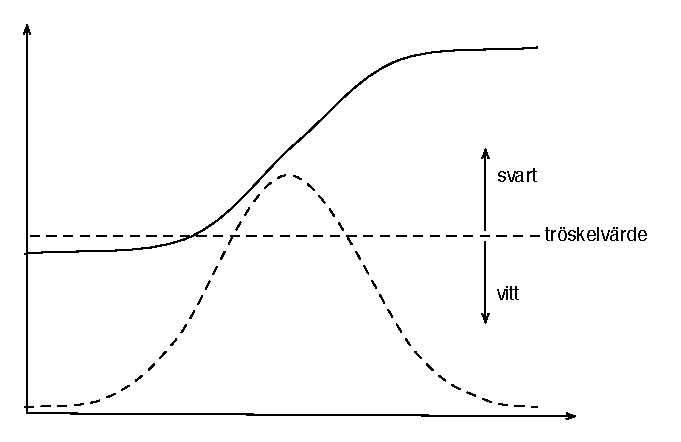
\includegraphics[width=\textwidth]{../img/w13-assignment-imageprocessing/derivatabild2.pdf}
\caption { En funktion (heldragen linje) och dess derivata (streckad linje).}
\label{fig:derivatabild}
\end{figure}

I figur~\ref{fig:derivatabild} visas en funktion $f$ (heldragen linje) och funktionens derivata $f'$ (streckad linje). Vi ser att där funktionen gör ett ''hopp'' så får derivatan ett stort värde. Om funktionen representerar intensiteten hos pixlarna längs en linje i x-led eller y-led så motsvarar ''hoppen'' en kontur i bilden. Om man sedan bestämmer sig för att pixlar där derivatans värde överstiger ett visst tröskelvärde ska vara svarta och andra pixlar vita så får man en bild med bara konturer. 

Nu är ju intensiteten hos pixlarna inte en kontinuerlig funktion som man kan derivera enligt vanliga matematiska regler. Men man kan approximera derivatan, till exempel med följande formel:

\begin{displaymath}
f'(x) \approx \frac{f(x+h) - f(x-h)}{2h}
\end{displaymath}

(Om man här låter $h$ gå mot noll så får man definitionen av derivatan.) Uttryckt i Scala och matrisen \code{intensity} så får man:

\begin{Code}
val derivative = (intensity(i)(j+1) - intensity(i)(j-1)) / 2
\end{Code}

Allt detta kan man uttrycka med hjälp av faltning. 

\begin{enumerate} 
	\item Beräkna intensitetsmatrisen med metoden \code{computeIntensity}.
	\item Falta varje punkt i intensitetsmatrisen med två kärnor:
$$
X\_SOBEL =
\begin{pmatrix}
  -1 & 0 & 1 \\
  -2 & 0 & 2 \\
  -1 & 0 & 1 \\
\end{pmatrix}
Y\_SOBEL =
\begin{pmatrix}
  -1 & -2 & -1 \\
  0 & 0 & 0 \\
  1 & 2 & 1 \\
\end{pmatrix}
$$
	Använd metoden \code{convolve} med vikten 1. Koefficienterna i matrisen $X\_SOBEL$ uttrycker derivering i x-led, i $Y\_SOBEL$ faltning i y-led. För att förklara varför koefficienterna ibland är 1 och ibland 2 måste man studera den bakomliggande teorin noggrant, men det gör vi inte här.
	\item Om resultaten av faltningen i en punkt betecknas med \code{sx} och \code{sy} så får man en indikator på närvaron av en kontur med \code{math.abs(sx) + math.abs(sy)}. Absolutbelopp behöver man eftersom man har negativa koefficienter i faltningsmatriserna. 
	\item  Sätt pixeln till svart om indikatorn är större än tröskelvärdet, till vit annars. Tröskelvärdet bestäms av \code{paramValue}. 
\end{enumerate}

Skriv en klass \code{SobelFilter} som implementerar denna algoritm.

\begin{figure}[H]
\begin{center}
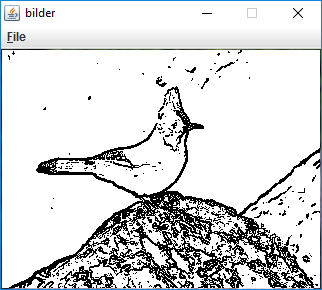
\includegraphics[scale=0.8]{../img/w13-assignment-imageprocessing/sobeljay.png}
\caption { Exempel på en bild där ett Sobelfilter applicerats med ett parametervärde på 150.}
\label{fig:sobel}
\end{center}
\end{figure}


\Task Implementera \code{FilterList} enligt specifikationerna ovan.

\Task Implementera \code{FilterChooser} enligt specifikationerna ovan.

\Task Knyt ihop allt i \code{ImageProcessing}-objektet som du skapade innan. Utskrifterna ska se ut på följande sätt:

{\setlength{\parindent}{0cm}

 Välj en av följande bilder genom att mata in en siffra\newline

0. boy.jpg\newline
1. car.jpg\newline
2. duck.jpg\newline
3. facade.jpg\newline
4. jay.jpg\newline
5. moon.jpg\newline
6. obidos.jpg\newline
7. sgrada.jpg\newline
8. shuttle.jpg\newline
Ditt val: 1\newline
Bild car.jpg laddad\newline
Tryck på 0 för Vanligt-filter\newline
Tryck på 1 för Blått-filter\newline
Tryck på 2 för Krypterat-filter\newline
Tryck på 3 för Inverterat-filter\newline
Tryck på 4 för Grått-filter\newline
Tryck på 5 för Kontrast-filter\newline
Tryck på 6 för Gauss-filter\newline
Tryck på 7 för Sobel-filter\newline
Tryck 42 om du inte vill använda fler filter\newline
Välj ett filter 1\newline
Välj ett filter 42\newline
Välja ny bild? (y/n) n\newline
}

Tänk på att användaren kan mata in otillåtna värden. Detta ska hanteras på lämpligt sätt.

\subsection{Frivilliga extrauppgifter}

\Task \textbf{Kontrastfilter.} Om man applicerar kontrastfiltrering på en färgbild så kommer bilden att konverteras till en gråskalebild. (Man kan naturligtvis förbättra kontrasten i en färgbild och få en färgbild som resultat. Då behandlar man de tre färgkanalerna var för sig.) Många bilder lider av alltför låg kontrast. Det beror på att bilden inte utnyttjar hela det tillgängliga området 0–255 för intensiteten. Man får en bild med bättre kontrast om man ''töjer ut'' intervallet enligt följande formel (lineär interpolation):

\begin{Code}
val newIntensity = 255 * (intensity - 45) / (225 - 45)
\end{Code}

Som synes kommer en punkt med intensiteten 45 att få den nya intensiteten 0 och en punkt med intensiteten 225 att få den nya intensiteten 255. Mellanliggande punkter sprids ut jämnt över intervallet \code{[0, 255]}. För punkter med en intensitet mindre än 45 sätter man den nya intensiteten till 0, för punkter med en intensitet större än 225 sätter man den nya intensiteten till 255. Vi kallar intervallet där de flesta pixlarna finns för \code{[lowCut, highCut]}. De punkter som har intensitet mindre än \code{lowCut} sätter man till 0, de som har intensitet större än \code{highCut} sätter man till 255. För de övriga punkterna interpolerar man med formeln ovan (45 ersätts med \code{lowCut}, 225 med \code{highCut}).

Det återstår nu att hitta lämpliga värden på \code{lowCut} och \code{highCut}. Detta är inte något som kan göras helt automatiskt, eftersom värdena beror på intensitetsfördelningen hos bildpunkterna. Man börjar med att beräkna bildens intensitetshistogram, dvs hur många punkter i bilden som har intensiteten 0, hur många som har intensiteten 1, . . . , till och med 255.

I de flesta bildbehandlingsprogram kan man sedan titta på histogrammet och interaktivt bestämma värdena på \code{lowCut} och \code{highCut}. Så ska vi dock inte göra här. I stället bestämmer vi oss för ett procenttal \code{cutOff} (som bestäms av \code{paramValue}) och beräknar \code{lowCut} så att \code{cutOff} procent av punkterna i bilden har en intensitet som är mindre än \code{lowCut} och \code{highCut} så att \code{cutOff} procent av punkterna har en intensitet som är större än \code{highCut}.

Exempel: antag att en bild innehåller 100 000 pixlar och att \code{cutOff} är 1.5. Beräkna bildens intensitetshistogram i en vektor
\begin{Code} 
val histogram = Array[Int](256)
\end{Code}

Beräkna \code{lowCut} så att \code{histogram(0)} + ... + \code{histogram(lowCut)} = 0.015 * 100000 (så nära det går att komma, det blir troligen inte exakt likhet). Beräkna \code{highCut} på liknande sätt.

Sammanfattning av algoritmen:
\begin{enumerate}
	\item Beräkna intensiteten hos alla punkterna i bilden, lagra dem i en \code{short}-matris. Använd den färdigskrivna metoden \code{computeIntensity}.
	\item Beräkna bildens intensitetshistogram.
	\item Parametervärdet \code{paramValue} är det värde som ska användas som \code{cutOff}.
	\item Beräkna \code{lowCut} och \code{highCut} enligt ovan.
	\item Beräkna den nya intensiteten för varje pixel enligt interpolationsformeln och lagra de nya pixlarna i \code{outPixels}.
\end{enumerate}
Skriv en klass \code{ContrastFilter} som implementerar algoritmen. I katalogen \emph{images} kan bilden \emph{moon.jpg} vara lämpliga att testa, eftersom den har låg kontrast. Anmärkning: om \code{cutOff} sätts = 0 så får man samma resultat av denna filtrering som man får av \code{GrayScaleFilter}. Detta kan man se genom att studera interpolationsformeln.


%!TEX encoding = UTF-8 Unicode

%!TEX root = ../compendium1.tex

%!TEX encoding = UTF-8 Unicode
\chapter{Muntlig examen}\label{chapter:W14}


%!TEX encoding = UTF-8 Unicode
%!TEX root = ../exercises.tex

\ifPreSolution

\Exercise{\ExeWeekFOURTEEN}\label{exe:W14}

\begin{Goals}
\item Känna till vad en tråd är och kunna förklara begreppet jämlöpande exekvering.
\item Känna till vad metoderna \code{run} och \code{start} gör i klassen \code{Thread}.
\item Kunna skapa och starta en tråd med överskuggad \code{run}-metod.
\item Kunna skapa ett enkelt program som från två trådar tävlar om att uppdatera en variabel och förklara varför beteendet kan bli oförutsägbart.
\item Kunna använda en \code{Future} för att köra igång flera parallella beräkningar.
\item Kunna registrera en callback på en \code{Future} med metoden \code{onComplete}.
%\item Känna till att webbsidor beskrivs av HTML-kod och kunna skapa en minimal webbsida.
%\item Kunna ladda ner en webbsida med \code{scala.io.Source.fromURL}.
\end{Goals}

% \begin{Preparations}
% \item \StudyTheory{14}
% \end{Preparations}

\else

\ExerciseSolution{\ExeWeekFOURTEEN}

\fi


\subsection{Frivilliga extrauppgifter}



\WHAT{Trådar.}

\QUESTBEGIN

\Task  \what~   Klassen \code{java.lang.Thread} används för att skapa  \textbf{trådar} med jämlöpande exekvering \Eng{concurrent execution}. På så sätt kan man få olika koddelar att köra samtidigt.

Klassen \code{Thread} definierar en tom \code{run}-metod. Vill man att tråden ska göra något vettigt får man överskugga \code{run} med det man vill ska göras.

En tråd körs igång med metoden \code{start} och då anropas automatiskt \code{run}-metoden och tråden exekverar koden i \code{run} jämlöpande med övriga trådar. Om man anropar \code{run} direkt blir det \emph{inte} jämlöpande exekvering.

\Subtask Skapa en tråd som gör något som tar lite tid och kör med \code{run} resp. \code{start}.
\begin{REPL}
def zzz = { print("zzzzzz"); Thread.sleep(5000); println(" VAKEN!")}
zzz
val t2 = new Thread{ override def run = zzz }
t2.run
t2.run; println("Gomorron!")
t2.start; println("Gomorron!")
t2.start
\end{REPL}

\Subtask Vad händer om man anropar \code{start} mer än en gång på samma tråd?

\Subtask Skapa två trådar med överskuggade \code{run}-metoder och kör igång dem samtidigt enligt nedan. Vilken ordning skrivs hälsningarna ut efter rad 3 resp. rad 4 nedan? Förklara vad som händer.
\begin{REPL}
val g = new Thread{ override def run = for (i <- 1 to 100) print("Gurka ") }
val t = new Thread{ override def run = for (i <- 1 to 100) print("Tomat ") }
g.run; t.run
g.start; t.start
\end{REPL}

\Subtask Använd \code{Thread.sleep} enligt nedan. Är beteendet helt förutsägbart (deterministiskt)? Förklara vad som händer. Du kan (om du kör Linux) avbryta REPL med Ctrl+C%
\footnote{\href{http://stackoverflow.com/questions/6248884/can-i-stop-the-execution-of-an-infinite-loop-in-scala-repl}{stackoverflow.com/questions/6248884/can-i-stop-the-execution-of-an-infinite-loop-in-scala-repl}}.
\begin{REPL}
def ibland(block: => Unit) = new Thread {
  override def run = while(true) { block; Thread.sleep(600) }
}.start
ibland(print("zzz ")); ibland(print("snark ")); ibland(println("hej!"))
\end{REPL}


\SOLUTION


\TaskSolved \what
     %%%TODO number  1 %%%starts with: \emph{Trådar.}  %%%

\SubtaskSolved   -

\SubtaskSolved  \code {java.lang.IllegalThreadStateException}. Det går inte att starta en tråd mer än en gång. Tråden kan därför inte startas om när den redan har exekverats.

\SubtaskSolved   När \code {start} anropas exekveras koden i \code{run} parallellt. Därför skrivs \code{Gurka} och \code{Tomat} ut omlöpande. Om istället \code{run} anropas direkt blir det inte jämnlöpande exekvering och \code{Gurka} skrivs ut 100 gånger, sedan skrivs \code{Tomat} ut 100 gånger.

\SubtaskSolved   \code{Thread.sleep} pausar inte tråden i exakt den tiden som angets. Alltså kommer det skrivas ut \code{zzz snark hej!} i de flesta fall, men det är inte garanterat.



\QUESTEND






\WHAT{Jämlöpande variabeluppdatering.}

\QUESTBEGIN

\Task \label{task:racecondition} \what~   Skriv klasserna \code{Bank} och \code{Kund} i en editor och klistra sedan in koden i REPL.

\begin{Code}
class Bank {
  private var saldo = 0;
  def visaSaldo: Unit = println("saldo: " + saldo)
  def sättIn: Unit = { saldo += 1 }
  def taUt: Unit   = { saldo -= 1 }
}

class Kund(bank: Bank) {
  def slösaSpara = {bank.taUt; Thread.sleep(1); bank.sättIn}
}
\end{Code}

\Subtask Använd funktionen \code{ibland} från föregående uppgift och kör nedan rader i REPL. Resultatet av jämlöpande variabeluppdatering blir här heltokigt och leder till mycket upprörda bankkunder och -ägare. Förklara vad som händer.

\begin{REPL}
val bank = new Bank
bank.visaSaldo
bank.sättIn
bank.visaSaldo
bank.taUt
bank.visaSaldo

val bamse = new Kund(bank)
val skutt = new Kund(bank)

bamse.slösaSpara
skutt.slösaSpara
bank.visaSaldo

def ofta(block: => Unit) = new Thread {
  override def run = while(true) { block; Thread.sleep(1) }
}.start

ofta(bamse.slösaSpara); ofta(skutt.slösaSpara)

ibland(bank.visaSaldo)
\end{REPL}


\SOLUTION


\TaskSolved \what
     %%%TODO number  2 %%%starts with: \emph{Jämlöpande variabeluppdat%%%

\SubtaskSolved  I \code{slösaSpara} hämtas saldot, ändras och placeras tillbaka i minnet -  fördröjs -  upprepas. Om \code{bamse} blir klar med att ladda, ändra och lagra innan skutt gör detsamma med den muterbara variablen hade det inte varit perfekt. Problemet ligger i  när en tråd laddar och innan den kan lagra det förändrade värdet laddar den andra tråden samma värde. Bara en av dessa trådar vinner racet och får lagra sitt ändrade tal. \code{skutt} och \code{bamse} blir alltså upprörda för att inte alla dess uttag och insättningar registreras.


\QUESTEND






\WHAT{Trådsäkra \code{AtomicInteger}.}

\QUESTBEGIN

\Task  \what~  Det finns stöd i JVM för att åstadkomma uppdateringar som inte kan avbrytas av andra trådar under pågånde minnesskrivning. En operation som inte kan avbrytas kallas \textbf{atomär} \Eng{atomic}. Studera dokumentationen för \code{AtomicInteger}\footnote{\href{https://docs.oracle.com/javase/8/docs/api/java/util/concurrent/atomic/AtomicInteger.html}{docs.oracle.com/javase/8/docs/api/java/util/concurrent/atomic/AtomicInteger.html}} och prova nedan kod. Förklara vad som händer.

Använd funktionerna \code{ofta} och \code{ibland} från tidigare uppgifter.
\begin{Code}
class SäkerBank {
  import java.util.concurrent.atomic.AtomicInteger
  private var saldo = new AtomicInteger
  def visaSaldo: Unit = println(s"saldo: ${saldo.get}")
  def sättIn: Unit = { saldo.incrementAndGet }
  def taUt: Unit   = { saldo.decrementAndGet }
}

class SäkerKund(bank: SäkerBank) {
  def slösaSpara = {bank.taUt; Thread.sleep(1); bank.sättIn}
}
\end{Code}
\begin{REPL}
val säkerBank = new SäkerBank
val farmor = new SäkerKund(säkerBank)
val vargen = new SäkerKund(säkerBank)

ofta(farmor.slösaSpara); ofta(vargen.slösaSpara)

ibland(säkerBank.visaSaldo)
\end{REPL}





\SOLUTION


\TaskSolved \what
     %%%TODO number  3 %%%starts with: \emph{Jämlöpande exekvering med%%%

Nu är \code{farmor} garanterad att kunna ladda saldot, ta ut pengar/ändra och lagra innan \code{vargen} kan överskriva resultatet. I \code{slösaSpara} pausas tråden i en millisekund så \code{vargen} kan fortfarande ta ut pengar innan \code{farmor} hinner sätta in pengar igen. Dock kommer alla uttag och insättningar registreras eftersom operationerna är atomära.


\QUESTEND






\WHAT{Jämlöpande exekvering med \code{scala.concurrent.Future}.}

\QUESTBEGIN

\Task \label{task:future} \what~   Att skapa och hålla reda på trådar kan bli ganska omständligt och knepigt att få rätt på.
Med hjälp av \code{scala.concurrent.Future} kan man på ett enklare sätta skapa jämlöpande exekvering.

\begin{Background}
Med en \code{Future} skapas jämlöpande exekvering som ''under huven'' använder ett ramverk som heter Akka\footnote{\url{http://akka.io/}}, skrivet i Scala och Java. Akka erbjuder automatisk  multitrådning med s.k. trådpooler och möjliggör avancerad parallellprogrammering på en hög  abstraktionsnivå, där man själv slipper skapa instanser av klassen \code{Thread}. I stället kan man helt enkelt placera sin kod inramad med \code|Future{ "körs parallellt" }| efter att man importerat det som behövs.
\end{Background}

\Subtask För att skapa jämlöpande exekvering med \code{Future} behöver man först göra import enligt nedan; då skapas ett exekveringssammanhang med trådpooler redo för användning. Starta om REPL och studera felmeddelandet efter rad 1 nedan. Importera därefter enligt nedan. Vad har \code{f} för typ?
\begin{REPL}
scala> concurrent.Future { Thread.sleep(1000); println("En sekund senare!") }
scala> import scala.concurrent._
scala> import ExecutionContext.Implicits.global
scala> val f = Future { Thread.sleep(1000); println("En sekund senare!") }
\end{REPL}

\Subtask Skapa en procedur \code{printLater} enligt nedan som skriver ut argumentet efter slumpmässig tid. Förklara vad som händer nedan.
\begin{REPL}
scala> def printLater(a: Any): Unit =
         Future { Thread.sleep((math.random * 10000).toInt); print(a + " ") }
scala> (1 to 42).foreach(i => printLater(i)); println("alla är igång!")
\end{REPL}

\Subtask Skapa enligt nedan en \code{Future} som räknar ut hur många siffror det är i ett väldigt stort tal. Med \code{onComplete} kan man ange vad som ska göras när den tunga beräkningen är färdig; detta kallas att ''registrera en callback''. Vilken returtyp har \code{big}? Hur många siffror har det stora talet? Vad har \code{r} för typ? Justera argumentet till \code{big} om du inte orkar vänta på resultatet...

\begin{REPL}
scala> BigInt(10).pow(100)
scala> BigInt(10).pow(100).toString.size
scala> def big(n: Int) = Future { BigInt(n).pow(n).toString.size }
scala> big(1234567).onComplete{r => println(r + " siffror") }
\end{REPL}

\Subtask Den stora vinsten med \code{Future} är att man kan köra vidare under tiden, varför anropet av \code{Future} kallas \textbf{icke-blockerande} \Eng{non-blocking}. Det händer ibland att man ändå vill blockera exekveringen i väntan på ett resultat. Man kan då använda objektet \code{scala.concurrent.Await} och dess metod \code{result} enligt nedan. Använd \code{big} från föregående uppgift och gör en blockerande väntan på resultatet enligt nedan. Vad händer? Vad händer om du väntar för kort tid?

\begin{REPL}
scala> import scala.concurrent.duration._
scala> Await.result(big(1234567), 20.seconds)
\end{REPL}



\SOLUTION


\TaskSolved \what
     %%%TODO number  4 %%%starts with: TODO  %%%%%%%%%%%%%%%%%%%\Advan%%%

\SubtaskSolved  error: Cannot find an implicit ExecutionContext. Future behöver en ExecutionContext för att kunna köras. \code{f} är av typen Future[Unit].

\SubtaskSolved  Funktionen \code{printLater} har en Future, vilket innebär att när både \code{printLater} och \code{println} anropas i foreach-loopen exekveras dom jämnlöpande. Eftersom det tar längre tid att starta upp en Future för datorn är \code{println} snabbare och skriver ut att alla är igång först. Sedan skrivs siffrorna från 1 - 42 ut med oregelbundna mellanrum eftersom tråden pausas olika länge.

\SubtaskSolved  \code{big} är en Future[Int]. Det stora talet har 7 520 383 siffror. \code{r} är av typen Try[Int] (se dokumentationen för Future om du är osäker)

\SubtaskSolved  Eftersom exekveringen blockas tills den har fått ett resultat går det inte att fortsätta skriva i REPL medan uträkningen pågår. Väntar man för kort tid får man ett TimeOutException och uträkningen avbryts.


\QUESTEND






\WHAT{Använda \code{Future} för att göra flera saker samtidigt.}

\QUESTBEGIN

\Task  \what~
I denna uppgift ska du ladda ner webbsidor parallellt med hjälp av \code{Future}, så att en nedladdning kan avslutas under tiden en annan dröjer.

\Subtask Koden för en minimal webbsida ser ut som nedan. Du kan beskåda sidan här: \url{http://fileadmin.cs.lth.se/pgk/mini.html} eller skriva in nedan kod i en fil som heter något som slutar på \texttt{.html} och öppna filen i din webbläsare.

\begin{verbatim}
<!DOCTYPE html>
<html>
<body>
HELLO WORLD!
</body>
</html>
\end{verbatim}

\Subtask För att simulera slöa webbservrar kan man ladda ner en sida via sajten \texttt{http://deelay.me/}. Ladda ner ovan sida med 2 sekunders fördröjning:\\
\url{http://deelay.me/2000/http://fileadmin.cs.lth.se/pgk/mini.html}

\Subtask Man kan ladda ner webbsidor med \code{scala.io.Source}. Vad händer nedan? Försök, med ledning av hur \code{delay} beräknas, uppskatta hur lång tid du måste vänta i medeltal, i bästa fall, respektive värsta fall, innan du kan se första webbsidan i vektorn \code{laddningar} nedan?

\begin{REPL}
scala> def ladda(url: String) = scala.io.Source.fromURL(url).getLines.toVector
scala> def slöladda(url: String) = {
         val delay = (math.random * 1000 + 2000).toInt
         val delaySite = s"http://deelay.me/$delay/"
         ladda(delaySite+url)
      }
scala> ladda("http://fileadmin.cs.lth.se/pgk/mini.html")
scala> def seg = slöladda("http://fileadmin.cs.lth.se/pgk/mini.html")
scala> val laddningar = Vector.fill(10)(seg)
scala> laddningar(0)
\end{REPL}

\Subtask Innan vi kan köra igång en \code{Future} så måste vi, som visats i uppgift \ref{task:future} importera den underliggande exekveringsmiljön som är redo att parallelisera ditt program i trådar utan att du själv måste skapa dem. Vad händer nedan?
\begin{REPL}
scala> import scala.concurrent._
scala> import ExecutionContext.Implicits.global
scala> val f = Future{ seg }
scala> f   // kolla om den är klar annars prova igen senare
scala> f
\end{REPL}

\Subtask Ladda indata utan att blockera \Eng{non-blocking input}. Förklara vad som händer nedan.
\begin{REPL}
scala> val nonblock = Future{ Vector.fill(10)(seg) }
scala> nonblock   // kolla igen senare om ej klar
scala> nonblock
\end{REPL}

\Subtask Ladda indata separat i olika parallella trådar. Förklara vad som händer nedan. Kör uttrycket på rad 3 nedan upprepade gånger i snabb följd efter varandra med pil-upp+Enter i REPL.
\begin{REPL}
scala> val para = Vector.fill(10)(Future{ seg })
scala> para
scala> para.map(_.isCompleted)
scala> para.map(_.isCompleted) // studera hur de blir färdiga en efter en
scala> para(0)
\end{REPL}

\Subtask Registrera en callback med metoden \code{onComplete}. Förklara vad som händer nedan.

\begin{REPL}
scala> val action = Vector.fill(10)(Future{ seg })
scala> action(0).onComplete(xs => println(s"ready:$xs"))
scala> // vänta tills laddning på plats 0 är klar
\end{REPL}

\Subtask Registrera en callback för felhantering i händelse av undantag med metoden \code{onFailure}. Förklara vad som händer nedan.
\begin{REPL}
scala> def lycka  = { Thread.sleep(3000); println(":)") }
scala> def olycka = { Thread.sleep(3000); 42 / 0; lycka }
scala> Future{ lycka  }.onFailure{ case e => println(s":( $e") }
scala> Future{ olycka }.onFailure{ case e => println(s":( $e") }
\end{REPL}



\SOLUTION


\TaskSolved \what
     %%%TODO number  5 %%%starts with: Sök upp och studera dokumentati%%%

\SubtaskSolved  -

\SubtaskSolved  -

\SubtaskSolved  Varje sida fördröjs med mellan 2 upp till 3 sekunder (2000-3000 millisekunder). Så i medeltal tar det 2.5 sekunder för varje sida att laddas. Vektorn måste fyllas innan exekveringen kan fortsätta. Därför laddas alla 10 stycken sidor in innan man kan se första websidan. Det tar därför i medeltal 2.5 x 10 = 25 sekunder.

\SubtaskSolved  \code{f} ger en Vektor fylld med strängar där varje element ges av en rad på hemsidan. Då \code{f} körs i bakgrunden kan programmet fortlöpa medan innehållet räknas ut. Du kan därför skriva \code{f} i REPL:n men det är inte säkert att proccessen är klar och det slutgilltiga resultatet visas.

\SubtaskSolved  Samma som ovan, förutom att det blir en vektor där varje element är i sig en vektor med strängar.

\SubtaskSolved  Laddar in datan parallelt så nedladdingen sker samtidigt, men det går olika snabbt pga metoden seg.

\SubtaskSolved  Eftersom datan laddas i parallella trådar utan blockering blir dom inte klara i ordning, utan i den ordningen tråden körs klart. Till slut blir alla klara och resultatet visar en vektor med \code{true} värden.

\SubtaskSolved  Metoden \code{lycka} är väldefinerad och kastar därför inga undantag. Den skriver alltid ut \code{:)}. Metoden \code{olycka} är inte väldefinerad då division med 0 ger \code{java.lang.ArithmeticException}. Detta fångas upp vid callbacken och det skrivs ut \code{:(} samt det specifierade undantaget.

\ExtraTasks %%%%%%%%%%%%


\QUESTEND






\WHAT{}

\QUESTBEGIN

\Task  \what~ Räkna ut stora primtal parallellt genom att använda nedan funktioner. Implementera \code{isPrime} enligt pseudokod från den engelska wikipediasidan om primtalstest\footnote{\href{https://en.wikipedia.org/wiki/Primality_test}{en.wikipedia.org/wiki/Primality\_test}} med den s.k. ''naiva algoritmen''.  Räkna ut 10 st slumpvisa primtal med 16 siffror vardera. Gör beräkningarna parallellt med hjälp av \code{Future}.

\begin{Code}
def isPrime(n: BigInt): Boolean = ???

def nextPrime(start: BigInt): BigInt = {
  var i = start
  while (!isPrime(i)) { i += 1 }
  i
}

def randomBigInt(nDigits: Int): BigInt = {
   def rndChar = ('0' + (math.random * 10).toInt).toChar
   val str = Array.fill(nDigits)(rndChar).mkString
   BigInt(str)
}
\end{Code}

\SOLUTION


\TaskSolved \what
  %%%TODO number  6 %%%

\begin{Code}
def isPrime(n: BigInt): Boolean = n match {
  case _ if (n <= 1) => false
  case _ if (n <= 3) => true
  case _ if n % 2 == 0 || n % 3 == 0 => false
  case _ =>
    var i = BigInt(5)
    while (i * i < n) {
      if (n % i == 0 || n % (i + 2) == 0) false
      i += 6
    }
    true
}

import scala.concurrent._
import ExecutionContext.Implicits.global

val primes = Vector.fill(10)(Future{nextPrime(randomBigInt(16))})
primes.foreach(_.onSuccess{case i => println(i)})
\end{Code}


\QUESTEND






\WHAT{Svara på teorifrågor.}

\QUESTBEGIN

\Task  \what~\Pen

\Subtask Vad är en tråd?

\Subtask Hur skapar man en tråd med klassen \code{Thread}?

\Subtask Hur startar man en tråd?

\Subtask Vilka problem kan man råka ut för om man uppdaterar samma resurs i flera olika trådar?

\Subtask Vad innbär det att kod är \emph{trådsäker}?

\Subtask Nämn några fördelar med att använda Future jämfört med att använda trådar direkt.


\SOLUTION


\TaskSolved \what
 %%%TODO number  7 %%%

\SubtaskSolved  Stackoverflow ger följande förklaring:

A thread is an independent set of values for the processor registers (for a single core). Since this includes the Instruction Pointer (aka Program Counter), it controls what executes in what order. It also includes the Stack Pointer, which had better point to a unique area of memory for each thread or else they will interfere with each other.

\SubtaskSolved

\begin{Code}
val thread = new Thread(new Runnable{
	def run(){println(''Det här är en tråd'')}
})
\end{Code}

\SubtaskSolved  \code{thread.start}

\SubtaskSolved  Det kan bli kapplöpning(race conditions) om vilken tråds resurser blir sparade. Vilket leder till att de andra trådarnas ändringar blir ignorerade.

\SubtaskSolved  Trådsäkerhet innebär att flera trådar kan köras parallellt utan felaktigheter i resultatet. Exempelvis får man vara väldigt försiktig om man vill ha en muterbar variabel som alla trådar ska ändra samtidigt.

\SubtaskSolved  Till exempel slipper man skapa instanser av klassen Thread eftersom man kan placera koden i en Future istället. Den löser även mycket under huven för kodaren.


\QUESTEND






\WHAT{Klasser med atomär uppdatering.}

\QUESTBEGIN

\Task  \what~ Läs om och testa klasserna AtomicBoolean, AtomicDouble och AtomicReference för atomär uppdatering i paketet \code{java.util.concurrent.atomic}. Använd några av dessa tillsammans med \code{scala.concurrent.Future}.


\SOLUTION

\TaskSolved --

\QUESTEND





\WHAT{Skapa din egen multitrådade webbserver.}

\QUESTBEGIN

\Task  \what~

\Subtask Skriv in\footnote{Eller ladda ner här: \href{https://github.com/lunduniversity/introprog/blob/master/compendium/examples/simple-web-server/webserver.scala}{github.com/lunduniversity/introprog/blob/master/compendium/examples/simple-web-server/webserver.scala}} nedan kod i en editor och spara i en fil med namn \texttt{webserver.scala} och kompilera och kör med \texttt{scala webserver.start} och beskriv vad som händer när du med din webbläsare surfar till adressen: \\ \url{http://localhost:8089/abbasillen}

\scalainputlisting[numbers=left,basicstyle=\ttfamily\fontsize{11}{12}\selectfont]{examples/simple-web-server/webserver.scala}

\Subtask Du ska nu skapa en webbserver som gör något lite mer intressant. Den ska svara med det 13:e Fibonacci-talet\footnote{\href{https://sv.wikipedia.org/wiki/Fibonaccital}{https://sv.wikipedia.org/wiki/Fibonaccital}} om du surfar till \url{http://localhost:8089/fib/13}.
Spara din webbserver från föregående deluppgift under det nya namnet \texttt{fibserver.scala} och använd koden nedan och lägg till och ändra så att din server kan svara med Fibonaccital. Vi börjar med att räkna ut Fibonaccital i funktionen \code{compute.fib} nedan på ett onödigt processorkrävande sätt med exponentiell tidskomplexitet så att webbservern verkligen får jobba, för att i senare deluppgifter implementera \code{compute.fib} med linjär tidskomplexitet och därmed undvika onödig planetuppvärmning.
\begin{CodeSmall}
  object compute {
    def fib(n: BigInt): BigInt = {
      if (n < 0) 0 else
      if (n == 1 || n == 2) 1
      else fib(n - 1) + fib(n -2)
    }
  }

  def fibResponse(num: String) = Try { num.toInt } match {
    case Success(n) => html.page(s"fib($n) == " + compute.fib(n))
    case Failure(e) => html.page(s"FEL $e: skriv heltal, inte $num")
  }

  def errorResponse(uri:String) = html.page("FATTAR NOLL: " + uri)

  def handleRequest(cmd: String, uri: String, socket: Socket): Unit = {
    val os = socket.getOutputStream
    val parts = uri.split('/').drop(1) // skip initial slash
    val response: String = (parts.head, parts.tail) match {
      case (head, Array(num)) => fibResponse(num)
      case _                  => errorResponse(uri)
    }
    os.write(html.header(response.size).getBytes("UTF-8"))
    os.write(response.getBytes("UTF-8"))
    os.close
    socket.close
  }
\end{CodeSmall}
Kör i terminalen med \texttt{scala fibserver.start} och beskriv vad som händer i din webbläsare när du surfar till servern.


%%%\textbf{KOD TILL FACIT:}
%%%\scalainputlisting[numbers=left,basicstyle=\ttfamily\fontsize{11}{12}\selectfont]{examples/simple-web-server/fibserver.scala}


\Subtask Surfa efter flera stora Fibonacci-tal samtidigt i olika flikar i din browser. Hur märks det att servern bara kör i en enda tråd?

\Subtask Gör din server multitrådad med hjälp av den nya server-loopen nedan.

\begin{CodeSmall}
import scala.concurrent._
import ExecutionContext.Implicits.global

  def serverLoop(server: ServerSocket): Unit = {
    println(s"http://localhost:${server.getLocalPort}/hej")
		while (true) {
  		Try {
  		  var socket = server.accept  // blocks thread until connect
	  	  val scan = new Scanner(socket.getInputStream, "UTF-8")
		    val (cmd, uri) = (scan.next, scan.next)
			  println(s"Request: $cmd $uri")
		    Future { handleRequest(cmd, uri, socket) }.onFailure {
		      case e => println(s"Reqest failed: $e")
		    }
		  }.recover{ case e: Throwable => s"Connection failed: $e" }
		}
  }
\end{CodeSmall}

\Subtask Surfa efter flera stora Fibonacci-tal samtidigt i olika flikar i din browser. Hur märks det att servern är multitrådad?


\Subtask Det är onödigt att räkna ut samma Fibonacci-tal flera gånger. Med hjälp av en cache i form av en föränderlig \code{Map} kan du spara undan redan uträknade värden. Det funkar dock inte med en vanlig \code{scala.collection.mutable.Map} i vår multitrådade webbserver, eftersom den inte är \textbf{trådsäker} \Eng{thread-safe}. Med trådosäkra föränderliga datastrukturer blir det samma besvärliga beteende som i uppgift \ref{task:racecondition}.

Du ska i stället använda \code{java.util.concurrent.ConcurrentHashMap}. Sök upp  dokumentationen för \code{ConcurrentHashMap} och försök förstå koden nedan. Hur fungerar metoderna \code{containsKey}, \code{put} och \code{get}?
\begin{Code}
object compute {
  import java.util.concurrent.ConcurrentHashMap
  val memcache = new ConcurrentHashMap[BigInt, BigInt]

  def fib(n: BigInt): BigInt =
    if (memcache.containsKey(n)) {
      println("CACHE HIT!!! no need to compute: " + n)
      memcache.get(n)
    } else {
      println("cache miss :( must compute fib:  " + n)
      val f = fastFib(n)
      memcache.put(n, f)
      f
    }

  private def fastFib(n: BigInt): BigInt = {
    if (n < 0) 0 else
    if (n == 1 || n == 2) 1
    else fib(n - 1) + fib(n -2)
  }
}
\end{Code}

\Subtask Använd ovan \code{fib}-objekt i en ny version av din webserver. Spara den i en ny kodfil med namnet \texttt{fibserver-memcached.scala}. Undersök hur snabbt det går med stora Fibonaccital med den nya varianten. Hur stora tal kan du räkna ut? Kan servern fortsätta efter överflödad stack? Förklara varför.

\Subtask Nu när vi kan få väldigt stora Fibonacci-tal kan det vara användbart att stoppa in radbrytningar på webbsidan. Html-taggen \texttt{</br>} ger en radbrytning.
\begin{Code}
  def insertBreak(s: String, n: Int = 80): String = {
    if (s.size < n) s
    else s.take(n) + "</br>" + insertBreak(s.drop(n),n)
  }
\end{Code}
Använd den rekursiva funktionen ovan för att pilla in radbrytningstaggar på var $n$:te position i långa strängar. Testa hur det ser ut på webbsidan med ovan funktion när din server svarar med väldigt stora tal.

\Subtask Vi ska nu använda det större heap-minnet i stället för stack-minnet och därmed inte begränsas av stackens max-storlek. Skriv om \code{fastFib} så att den använder en \code{while}-sats i stället för ett rekursivt anrop. Denna uppgift är ganska klurig, men om du kör fast kan du snegla i lösningarna i Appendix för inspiration.

Hur stora tal klarar din server nu? Vad händer med servern när minnet tar slut? Hur kan du skydda servern så att den inte kan hänga sig?

\SOLUTION


\TaskSolved \what
 %%%TODO number  9 %%%

\SubtaskSolved  \code{abbasillen} skrivs ut baklänges till \code{nellisabba}.

\SubtaskSolved

\SubtaskSolved

\SubtaskSolved

\SubtaskSolved

\SubtaskSolved

\SubtaskSolved

\SubtaskSolved

\SubtaskSolved

Lösningsförslag:
\scalainputlisting[numbers=left,basicstyle=\ttfamily\fontsize{11}{12}\selectfont]{examples/simple-web-server/fibserver-threaded-memcached-while.scala}


\QUESTEND






\WHAT{}

\QUESTBEGIN

\Task  \what~ Utöka din server med fler beräkningsintensiva funktioner. Exempelvis primtalsberäkningar eller beräkningar av valfritt antal decimaler av $\pi$ eller $e$. Utnyttja gärna det du lärt dig i  matematiken om summor och serieutvecklingar.

\SOLUTION


\TaskSolved \what
 %%%TODO number  10 %%%

---


\QUESTEND






\WHAT{}

\QUESTBEGIN

\Task  \what~ Läs mer om \code{Future} och jämlöpande exekvering i Scala här:\\
\href{http://alvinalexander.com/scala/future-example-scala-cookbook-oncomplete-callback}{alvinalexander.com/scala/future-example-scala-cookbook-oncomplete-callback}

\SOLUTION


\TaskSolved \what
 %%%TODO number  11 %%%

---


\QUESTEND






\WHAT{}

\QUESTBEGIN

\Task  \what~ Läs mer om jämlöpande exekvering och multitrådade program i Java här: \href{http://www.tutorialspoint.com/java/java_multithreading.htm}{www.tutorialspoint.com/java/java\_multithreading.htm}  \\
\noindent När man skriver program med jämlöpande exekvering finns det många fallgropar; det kan bli kapplöpning \Eng{race conditions} om gemensamma resurser och dödläge \Eng{deadlock} där inget händer för att trådar väntar på varandra. Mer om detta i senare kurser.


\SOLUTION


\TaskSolved \what
 %%%TODO number  12 %%%

---


\QUESTEND






\WHAT{Studera dokumentationen i \code{scala.concurrent}.}

\QUESTBEGIN

\Task  \what~\Pen

\Subtask Studera dokumentationen för \code{scala.concurrent.Future}\footnote{\href{http://www.scala-lang.org/files/archive/api/current/\#scala.concurrent.Future}{http://www.scala-lang.org/files/archive/api/current/\#scala.concurrent.Future}}. Hur samverkar \code{Future} med \code{Try} och \code{Option}? Vilka vanliga samlingsmetoder känner du igen?

\Subtask Studera dokumentationen för \code{scala.concurrent.duration.Duration}\footnote{\href{http://www.scala-lang.org/api/current/\#scala.concurrent.duration.Duration}{www.scala-lang.org/api/current/\#scala.concurrent.duration.Duration}}. Vilka tidsenheter kan användas?

\Subtask Vid import av \code{scala.concurrent.duration._ } dekoreras de numeriska klasserna med metoder för att skapa instanser av klassen \code{Duration}. Detta möjligörs med hjälp av klassen \code{scala.concurrent.duration.DurationConversions}. Studera dess dokumentation och testa att i REPL skapa några tidsperioder med metoderna på \code{Int}.



\SOLUTION


\TaskSolved \what
 %%%TODO number  13 %%%

\SubtaskSolved

\SubtaskSolved

\SubtaskSolved


\QUESTEND






\WHAT{}

\QUESTBEGIN

\Task  \what~ Fördjupa dig inom webbteknologi.

\Subtask Lär dig om HTML, CSS och JavaScript här: \url{https://developer.mozilla.org/en-US/docs/Learn}

\Subtask Lär dig om Scala.JS här: \url{http://www.scala-js.org/}\SOLUTION


\TaskSolved \what
 %%%TODO number  14 %%%

\SubtaskSolved  ---

\SubtaskSolved  ---

\SubtaskSolved  ---

\SubtaskSolved  ---
\QUESTEND

%!TEX encoding = UTF-8 Unicode
%%% EMPTY


\part{Appendix}
\appendix

\setcounter{chapter}{8} %next is I in \Alph

%!TEX encoding = UTF-8 Unicode
%!TEX root = ../compendium.tex

\chapter{Integrerad utvecklingsmiljö}\label{appendix:ide}

\section{Vad är en integrerad utvecklingsmiljö?}

En integrerad utvecklingsmiljö \Eng{integrated development environment, IDE} samlar ett flertal verktyg, inklusive en avancerad \textbf{editor} (se appendix \ref{appendix:edit}), för att skapa, köra och testa program. Det finns flera utvecklingsmiljöer att välja mellan, som kan användas för både Scala och Java.

En IDE ger stöd för \textbf{kodkomplettering} \Eng{code completion} där tillgängliga metoder visas i en lista och resten av ett namn kan fyllas efter att du skrivit de första bokstäverna i namnet. En IDE kan hjälpa dig med formattering och även skapa skelettkod utifrån \textbf{kodmallar} \Eng{code templates}. Med \textbf{felindikering} \Eng{error highlighting} får du understrykning av vissa fel direkt i koden och ibland kan du även få hjälp med förslag på åtgärder för att rätta till enkla fel. Funktioner för \textbf{avlusning} \Eng{debugging} hjälper dig att felsöka medan du kör din kod. Med funktioner för \textbf{omstrukturering} \Eng{refactoring} av kod får du hjälp av editorn i samarbete med kompilatorn att göra omfattande strukturförändringar i många kodfiler samtidigt, t.ex. namnbyten med hänsyn taget till språkets synlighetsregler.  

Alla dessa avancerade funktioner kan öka produktiviteten avsevärt, men samtidigt tar de tid att lära sig och en IDE kan kräva mycket datorkraft och viss väntetid jämfört med en vanlig, fristående editor. I början kan all funktionalitet upplevas som överväldigande och det kan vara svårt att hitta i alla menyer och inställningar. Ska man bara skriva ett litet, enkelt program, eller göra några mindre ändringar, är det många som föredrar en fristående, snabbstartad kodeditor före en fullfjädrad, tungrodd IDE. Å andra sidan kan en IDE med kodkomplettering vara till stor hjälp när man ska lära sig ett nytt api och experimentera med en okänd kodmassa.

I kursen använder vi flera utvecklingsmiljöer. På första labben använder vi Kojo (avsnitt \ref{appendix:ide:kojo}) som är en IDE speciellt anpassad på nybörjare. I laborationerna senare i kursen kan du välja att använda någon av de professionella utvecklingsmiljöerna Eclipse (avsnitt \ref{appendix:ide:eclipse}) eller IntelliJ (avsnitt \ref{appendix:ide:intellij}). Om du inte vet vilken du ska välja, börja med att prova Eclipse.


\newpage

\section{Kojo}\label{appendix:ide:kojo}

Kojo%
\footnote{\href{https://en.wikipedia.org/wiki/Kojo_(programming_language)}{en.wikipedia.org/wiki/Kojo\_(programming\_language)}}
 är en integrerad utvecklingsmiljö för Scala som är speciellt anpassad för nybörjare i programmering. Kojo används i LTH:s Science Center Vattenhallen för utbildning av grundskolelärare i programmering och vid skolbesök och annan besöksverksamhet, i vilken lärare och studenter vid LTH arbetar som handledare. Kojo är fri öppenkällkod och utvecklingen leds av Lalit Pant.

Kursens första laboration genomförs med hjälp av Kojo, men Kojo kan med fördel användas som komplement till Scala REPL och annan IDE under hela kursens gång. Medan Scala REPL lämpar sig för korta kodsnuttar, och en fullfjädrad, professionell IDE har funktioner för att hantera riktigt stora programmeringsprojekt, passar Kojo bra för mellanstora program. I Kojo finns även lätttillgängliga bibliotek som gör tröskeln lägre att programmera rörlig grafik och enkla spel.   


\begin{figure}[H]
\centering
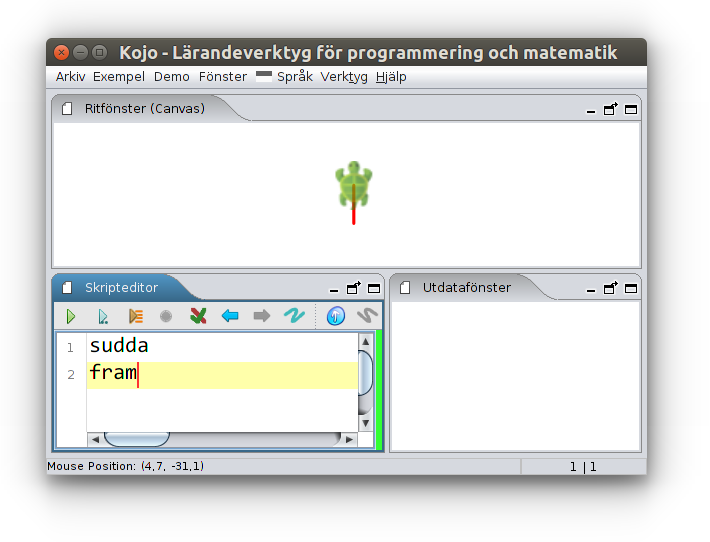
\includegraphics[width=0.8\textwidth]{../img/kojo/kojo.png}
\caption{Den nybörjarvänliga utvecklingsmiljön Kojo för Scala på svenska.}
\label{fig:appendix:ide:kojo}
\end{figure} 

\subsection{Installera Kojo}

Kojo är förinstallerat på LTH:s datorer och körs igång med kommandot \texttt{kojo}. För instruktioner om hur du installerar Kojo på din egen dator se här:\\
\href{http://www.lth.se/programmera/installera/}{lth.se/programmera/installera}

Kojo kräver att \texttt{java} finns på din dator. Eftersom du behöver tillgång till JDK i kursen, är det lika bra att installera hela JDK direkt (och inte bara JRE, så som beskrivs å länken ovan); se vidare hur du gör detta i avsnitt \ref{appendix:compile:install-jdk}. 
%\href{http://www.kogics.net/kojo-download}{www.kogics.net/kojo-download}


\subsection{Använda Kojo}

När du startar Kojo första gången, välj ''Svenska'' i språkmenyn och starta om Kojo. Därefter fungerar grafikfunktionerna på svenska enligt tabell \ref{table:kojo:functions}. När du startat om Kojo inställt på Svenska ser programmet ut ungeför som i figur \ref{fig:appendix:ide:kojo} på sidan \pageref{fig:appendix:ide:kojo}.


Det finns ett antal användbara kortkommando som du hittar i menyerna i Kojo. Undersök speciellt Ctrl+Alt+Mellanslag som ger autokomplettering baserat på det du börjat skriva.


{\small\renewcommand{\arraystretch}{1.45}
\begin{longtable}{@{}p{0.42\textwidth} p{0.55\textwidth}}

\caption{Några av sköldpaddans funktioner. Se även \href{http://lth.se/programmera}{lth.se/programmera}}\label{table:kojo:functions}\\

\emph{Svenska/Engelska} & \emph{Vad händer?}  \\ \hline
%!TEX encoding = UTF-8 Unicode
%!TEX root = ../compendium2.tex

\chapter{Kojo}\label{appendix:kojo}

\section{Vad är Kojo?}

Kojo%
\footnote{\href{https://en.wikipedia.org/wiki/Kojo_(programming_language)}{en.wikipedia.org/wiki/Kojo\_(programming\_language)}}
 är en integrerad utvecklingsmiljö för Scala som är speciellt anpassad för programmeringsundervisning i grundskolan. Kojo används i LTH:s Science Center Vattenhallen för utbildning av grundskolelärare i programmering och vid skolbesök och annan besöksverksamhet, i vilken lärare och studenter vid LTH arbetar som handledare. 
 
 Kojo är öppen källkod och utvecklingsgemenskapen leds av Lalit Pant från Indien. I Kojo finns även lättillgängliga bibliotek som gör tröskeln lägre att programmera rörlig grafik och enkla spel.

Under kursens första laboration använder vi grafikbiblioteket i Kojo för att illustrera grundläggande begrepp, så som sekvens, alternativ, repetition och abstraktion.  


\begin{figure}[H]
\centering
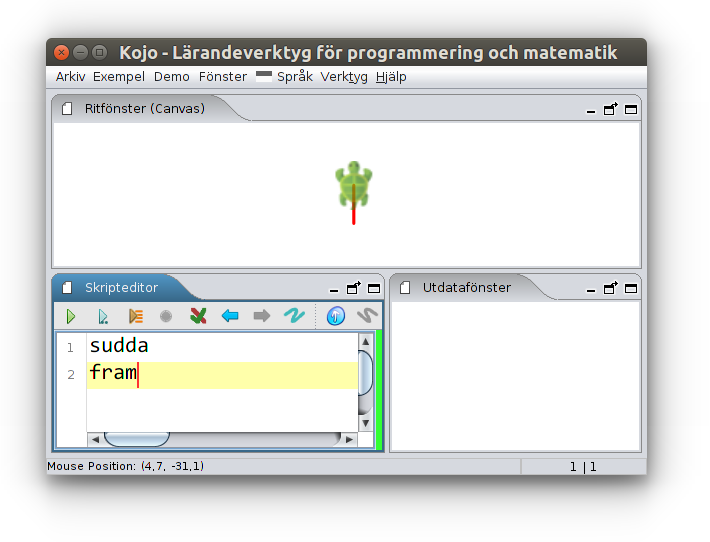
\includegraphics[width=0.8\textwidth]{../img/kojo/kojo.png}
\caption{Den nybörjarvänliga utvecklingsmiljön Kojo för Scala på svenska.}
\label{fig:appendix:ide:kojo}
\end{figure}

\section{Använda grafikbiblioteket i Kojo}\label{appendix:ide:kojo:install}

Kojo bygger på den beprövade pedagogiska idén med sköldpaddsgrafik \Eng{turtle graphics}\footnote{\url{https://en.wikipedia.org/wiki/Turtle_graphics}}, där du skriver program som styr en sköldpadda med en penna under magen. När sköldpaddan rör sig bildas ett streck av valfri färg på skärmen. Beroende på hur du bestämmer att sköldpaddan ska röra sig och vilken färg du bestämmer att pennan ska ha, kan du skapa olika intressanta bilder och samtidigt lära dig om programmeringens grunder.

Under kursens första laboration ska du använda grafikbiblioteket i Kojo tillsammans med editorn VS \code{code} och \code{scala-cli} i terminalen (se appendix \ref{appendix:terminal} och \ref{appendix:compile}). Ladda ner filen \texttt{kojo.scala} från \url{https://cs.lth.se/pgk/kojolib} och spara i en ny katalog med hjälp av din webbläsare, eller via dessa kommandon:

\begin{REPLnonum}
> mkdir w01-kojo
> cd w01-kojo
> curl -o kojolib.scala -sL https://cs.lth.se/pgk/kojolib
\end{REPLnonum}

Nu kan du starta Scala REPL och rita med Kojo så här:

\begin{REPLnonum}
> scala-cli repl .
Welcome to Scala 3.1.2 (17.0.2, Java OpenJDK 64-Bit Server VM).
Type in expressions for evaluation. Or try :help.
                                                                                                                               
scala> fram; höger; fram; vänster

\end{REPLnonum}

Du kan starta VS \code{code} i aktuellt bibliotek så här:
\begin{REPLnonum}
> code .
\end{REPLnonum}

Skriv nedan progam i VS \code{code} och spara det i samma katalog som den tidigare nedladdade filen, under ett nytt valfritt filnamn, t.ex. \code{rita.scala}:

\begin{Code}
@main def rita =
  fram; höger
  fram; vänster
\end{Code}

Kör ditt fristående program med:
\begin{REPLnonum}
> scala-cli run .
\end{REPLnonum}

Du ska nu få upp ett fönster som heter Kojo Canvas med en sköldpadda som ritat två streck. När du stänger fönstret så avslutas programmet. Prova fler sköldpaddsfunktioner enligt tabell \ref{table:kojo:functions}.

I stället för att ladda ned filen \code{kojolib.scala} så kan du placera dess innehåll på lämpligt ställe i ditt program enligt nedan. Observera att raden som börjar med \code{//> using lib} ska vara en enda lång rad utan radbrytningar. Raden med \code{export} gör Kojos kommandon tillgängliga utan prefix:
\begin{CodeSmall}[breaklines=true]
//> using scala "3"
//> using lib "net.kogics:kojo-lib:0.1.1,url=https://github.com/lunduniversity/introprog/releases/download/kojo-lib-0.1.1/kojo-lib-0.1.1.jar"

export net.kogics.kojo.Swedish.*, padda.*, CanvasAPI.*, TurtleAPI.*
\end{CodeSmall}


\noindent Scala-koden för den svenska paddans api finns här: \\
%\href{https://github.com/litan/kojo/blob/master/src/main/scala/net/kogics/kojo/lite/i18n/svInit.scala}{github.com/litan/kojo/blob/master/src/main/scala/net/kogics/kojo/lite/i18n/svInit.scala} \\
\href{https://github.com/litan/kojo-lib/blob/main/src/main/scala/net/kogics/kojo/i18n/Swedish.scala}{github.com/litan/kojo-lib/blob/main/src/main/scala/net/kogics/kojo/i18n/Swedish.scala}


%Kojo kräver (numera) \emph{inte} att \texttt{java} finns på din dator utan kommer med en egen JVM. 
%Eftersom du behöver tillgång till JDK i kursen, är det lika bra att installera hela JDK direkt (och inte bara JRE, så som beskrivs å länken ovan); se vidare hur du gör detta i avsnitt \ref{appendix:compile:install-jdk}.
%\href{http://www.kogics.net/kojo-download}{www.kogics.net/kojo-download}


{\small\renewcommand{\arraystretch}{1.4}
\begin{longtable}{@{}p{0.42\textwidth} p{0.55\textwidth}}

\caption{Ett urval av funktioner i Kojo. Se även \href{http://lth.se/programmera}{lth.se/programmera}}\label{table:kojo:functions}\\

\emph{Svenska/Engelska} & \emph{Vad händer?}  \\ \hline
\code|sudda| \newline \code|clear| & Ritfönstret suddas \\
\code|fram| \newline \code|forward()| & Paddan går framåt 25 steg. \\
\code|fram(100)| \newline \code|forward(100)| & Paddan går framåt 100 steg. \\
\code|höger| \newline \code|right(90)| & Paddan vrider sig 90 grader åt höger. \\
\code|höger(45)| \newline \code|right(45)| & Paddan vrider sig 45 grader åt höger. \\
\code|vänster| \newline \code|left(90)| & Paddan vrider sig 90 grader åt vänster. \\
\code|vänster(45)| \newline \code|left(45)| & Paddan vrider sig 45 grader åt vänster. \\
\code|hoppa| \newline \code|hop| & Paddan hoppar 25 steg utan att rita. \\
\code|hoppa(100)| \newline \code|hop(100)| & Paddan hoppar 100 steg utan att rita. \\
\code|hoppaTill(100, 200)| \newline \code|jumpTo(100, 200)| & Paddan hoppar till läget (100, 200) utan att rita. \\
\code|gåTill(100, 200)| \newline \code|moveTo(100, 200)| & Paddan vrider sig och går till läget (100, 200). \\
\code|hem| \newline \code|home| & Paddan går tillbaka till utgångsläget (0, 0). \\
\code|öster| \newline \code|setHeading(0)| & Paddan vrider sig så att nosen pekar åt höger. \\
\code|väster| \newline \code|setHeading(180)| & Paddan vrider sig så att nosen pekar åt vänster. \\
\code|norr| \newline \code|setHeading(90)| & Paddan vrider sig så att nosen pekar uppåt. \\
\code|söder| \newline \code|setHeading(-90)  | & Paddan vrider sig så att nosen pekar neråt. \\
\code|mot(100,200)| \newline \code|towards(100, 200)| & Paddan vrider sig så att nosen pekar mot läget (100, 200) \\
\code|sättVinkel(90)| \newline \code|setHeading(90)| & Paddan vrider nosen till vinkeln 90 grader. \\
\code|vinkel| \newline \code|heading| & Ger vinkelvärdet dit paddans nos pekar. \\
\code|sakta(5000)| \newline \code|setAnimationDelay(5000) | & Gör så att paddan ritar jättesakta. \\
\code|suddaUtdata| \newline \code|clearOutput| & Utdatafönstret suddas. \\
\code|utdata("hej")| \newline \code|println("hej")| & Skriver texten \texttt{hej} i utdatafönstret. \\
\code|val t = indata("Skriv")| \newline \code|val t = readln("Skriv:")| & Väntar på inmatning efter ledtexten \texttt{Skriv} och sparar den inmatade texten i t.  \\
\code|textstorlek(100)| \newline \code|setPenFontSize(100)| & Paddan skriver med jättestor text nästa gång du gör skriv. \\
\code|båge(100, 90)| \newline \code|arc(100, 90)| & Paddan ritar en båge med radie 100 och vinkel 90. \\
\code|cirkel(100)| \newline \code|circle(radie)| & Paddan ritar en cirkel med radie 100. \\
\code|synlig| \newline \code|visible| & Paddan blir synlig. \\
\code|osynlig| \newline \code|invisible| & Paddan blir osynlig. \\
\code|läge.x| \newline \code|position.x| & Ger paddans x-läge \\
\code|läge.y| \newline \code|position.y| & Ger paddans y-läge \\
\code|pennaNer| \newline \code|penDown| & Sätter ner paddans penna så att den ritar när den går. \\
\code|pennaUpp| \newline \code|penUp| & Lyfter upp paddans penna så att den INTE ritar när den går. \\
\code|pennanÄrNere| \newline \code|penIsDown| & Kollar om pennan är nere eller inte. \\
\code|färg(rosa)| \newline \code|setPenColor(pink)| & Sätter pennans färg till rosa. \\
\code|fyll(lila)| \newline \code|setFillColor(purple)| & Sätter ifyllnadsfärgen till lila. \\
\code|fyll(genomskinlig)| \newline \code|setFillColor(noColor)| & Gör så att paddan inte fyller i något när den ritar. \\
\code|bredd(20)| \newline \code|setPenThickness(20)| & Gör så att pennan får bredden 20. \\
\code|sparaStil| \newline \code|saveStyle| & Sparar pennans färg, bredd och fyllfärg. \\
\code|laddaStil| \newline \code|restoreStyle| & Laddar tidigare sparad färg, bredd och fyllfärg. \\
\code|sparaLägeRiktning| \newline \code|savePosHe| & Sparar pennans läge och riktning \\
\code|laddaLägeRiktning| \newline \code|restorePosHe| & Laddar tidigare sparad riktning och läge \\
\code|siktePå| \newline \code|beamsOn| & Sätter på siktet. \\
\code|sikteAv| \newline \code|beamsOff| & Stänger av siktet. \\
\code|bakgrund(svart)| \newline \code|setBackground(black)| & Bakgrundsfärgen blir svart. \\
\code|bakgrund2(grön,gul)| \newline \code|setBackgroundV(green, yellow)| & Bakgrund med övergång från grönt till gult. \\
\code|upprepa(4){fram; höger}| \newline \code|repeat(4){forward; right}| & Paddan går fram och svänger höger 4 gånger. \\
\code|avrunda(3.99)| & Avrundar 3.99 till 4.0 \\
\code|slumptal(100)| & Ger ett slumptal mellan 0 och 99. \\
\code|slumptalMedDecimaler(100)| & Ger ett slumptal mellan 0 och 99.99999999 \\
\code|systemtid| & Ger nuvarande systemklocka i sekunder. \\
\code|räknaTill(5000)| & Kollar hur lång tid det tar för din dator att räkna till 5000. \\


\end{longtable}
}%end small


\section{Kojo Desktop}

Kojo finns som fristående skrivbordsapplikation, kallad Kojo Desktop. Kojo Desktop innehåller en egen editor med syntaxfärgning för Scala, men fungerar ännu så länge bara för Scala 2. En av de synligaste skillnaderna mellan Scala 2 och Scala 3 är att klammerparenteser vid flerradiga funktioner är nödvändiga i Scala 2, medan Scala 3 har valfria klammerparenteser. Så om du använder Kojo Desktop behöver du komma ihåg att omgärda sekvenser av rader som hör ihop med \code|{| och \code|}|. 

Kojo Desktop är förinstallerat på LTH:s datorer och körs igång med terminalkommandot \texttt{kojo} eller via applikationsmenyn.  För instruktioner om hur du installerar Kojo Desktop på din egen dator se här: \href{http://www.lth.se/programmera/installera/}{lth.se/programmera/installera}

När du startar Kojo första gången, välj ''Svenska'' i språkmenyn och starta om Kojo. Därefter fungerar grafikfunktionerna på svenska enligt tabell \ref{table:kojo:functions}. När du startat om Kojo inställt på svenska ser programmet ut ungefär som i figur \ref{fig:appendix:ide:kojo} på sidan \pageref{fig:appendix:ide:kojo}.

Det finns ett antal användbara kortkommando som du hittar i menyerna i Kojo Desktop. Undersök speciellt Ctrl+Alt+Mellanslag som ger autokomplettering baserat på det du börjat skriva.

\section{Kojo i Webbläsaren}

En begränsad variant av Kojo finns tillgänglig för programmering direkt i din webbläsare här: \url{http://kojo.lu.se/}

När du trycker på play-knappen så kompileras din kod på en server till Javascript via ScalaJS och därefter körs Javascript-koden i din webbläsare. 
Kojo på webben är också ännu så länge begränsad till Scala 2 och kräver att du omgärdar sekvenser av rader som hör ihop med \code|{| och \code|}|.


\section{Mer om Kojo}

I detta dokument finns en enkel introduktion till Kojo: \\ ''Introduction to Kojo'' \url{http://www.kogics.net/kojo-ebooks#intro}


\hline
\end{longtable}
}%end small

\noindent Scala-koden för den svenska paddans api finns här: \\
\href{https://bitbucket.org/lalit_pant/kojo/src/tip/src/main/scala/net/kogics/kojo/lite/i18n/svInit.scala}{bitbucket.org/lalit\_pant/kojo/src/tip/src/main/scala/net/kogics/\\kojo/lite/i18n/svInit.scala}




\newpage

\section{Eclipse och ScalaIDE}\label{appendix:ide:eclipse}

Eclipse%
\footnote{\href{https://en.wikipedia.org/wiki/Eclipse_(software)}{en.wikipedia.org/wiki/Eclipse\_(software)}}
är en professionell IDE som stödjer många olika programmeringsspråk. Eclipse är skriven i Java och bygger vidare på ett utvecklingsprojekt som initierades av IBM. Eclipse är ett fritt och öppet projekt som numera kontrolleras av en oberoende stiftelse.

Till Eclipse finns en insticksmodul \Eng{plug-in} som kallas ScalaIDE och erbjuder stöd för Scala med tillhörande standardbibliotek.

Eclipse är en omfattande och avancerad programmeringsmiljö med många funktioner och inställningar. Det finns även en omfattande uppsättning insticksmoduler och tilläggsprogram som underlättar utveckling av t.ex. webbprogram, databaser och mycket annat. 

I detta avsnitt ges länkar till installation samt tips om hur du kommer igång med att använda Eclipse och ScalaIDE. Det går ganska snabbt att lära sig grunderna, men det kräven en viss ansträngning att lära sig de mer avancerade funktionerna. Det finns omfattande resurser på nätet som hjälper dig vidare. 


\subsection{Installera Eclipse Mars och ScalaIDE}\label{appendix:ide:eclipse:install}

Eclipse med ScalaIDE är förinstallerat på LTH:s datorer och startas med kommandot \texttt{scalaide} i ett terminalfönster.

ScalaIDE fungerar med Eclipse-versionerna \textit{Luna} och \textit{Mars} (men i skrivande stund fungerar ScalaIDE ännu \textit{inte} med den allra senaste versionen kallad \textit{Neon}). 

För att installera ScalaIDE på din egen dator, följ nedan instruktioner: 

\begin{enumerate}
\item Kontrollera enligt avsnitt \ref{appendix:compile:check-jdk} att du har \texttt{java} installerat och installera vid behov JDK enligt avsnitt \ref{appendix:compile:install-jdk}.

\item Installera Eclipse version \textbf{Mars}, varianten för \textbf{Java Developers} som återfinns på denna sida: \\ \url{https://www.eclipse.org/downloads/packages/release/Mars/2} \\ som är den \textit{andra} varianten i listan (alltså inte Java EE). Följ dessa steg:
\begin{enumerate}
\item Klicka på den \textbf{64-bit}-variant som passar ditt operativsystem.
\item Filen som laddas ner heter något som liknar (beroende på OS): \\ \texttt{eclipse-java-mars-2-win32-x86\_64.zip} 
\\ Det kan ta lång tid att ladda ner filen som är på ca 170MB. Om du klickar på \textit{''select a mirror''} kan du välja en svensk sajt för att ladda ner snabbare. 

\item Dubbelklicka på filen för att packa upp den, vilket kan ta många minuter. Du får, när upppackningen är klar, ett bibliotek med en fungerande Eclipse-installation som du kan placera var du vill. Kör du Windows, lägg den förslagsvis här:\\ 
\code|C:\eclipse\eclipse-java-mars-2-win32-x86_64|

\item för Ubuntu Linux finns kompletterande installationsanvisningar här, som ger dig en ikon i app-menyn m.m.: 
\\ \url{http://askubuntu.com/questions/26632/how-to-install-eclipse}
\end{enumerate}

\item Installera Scala IDE inifrån%
\footnote{Det finns på ScalaIDE-hemsidan möjlighet att ladda ner en Eclipse-variant med färdiginstallerad ScalaIDE-plugin, men då får du i skrivande stund den gamla versionen Eclipse \textit{Luna}, varför du rekommenderas att, enligt instruktionerna här, själv installera ScalaIDE inifrån Eclipse \textit{Mars}, som är den senaste Eclipse-versionen för vilken ScalaIDE fungerar.}
 Eclipse enligt nedan steg:
\begin{enumerate}
\item Starta Eclipse, t.ex. genom att köra igång den exekverbara filen som ligger i underbiblioteket \texttt{eclipse}, i Windows heter den \texttt{eclipse.exe} medan den exekverbara filen i Linux heter \texttt{eclipse} utan filändelse.

\item Välj i frågerutan som dyker upp, någon plats för \textit{workspace} (kvittar vilken just nu, kan ändras senare).

\item Klicka på menyn \textit{Help} $\rightarrow$ \textit{Install new software}.

\item Klicka på \textit{Add}-knappen till höger och skriv: \\ \textit{''ScalaIDE for Scala 2.11''} i \textit{Name}-fältet och ange denna adress i \textit{Location}-fältet: \\
  {\small\mbox{\url{http://download.scala-ide.org/sdk/lithium/e44/scala211/stable/site}}} \\
  och klicka \textit{OK}.
  
\item Du får nu upp en lista med alternativ. Kryssa för alternativet
\\ {\frame{\checkmark}}~~\textit{Scala IDE for Eclipse} \\ och klicka \textit{Next} och sedan \textit{Next} igen och acceptera licensvillkoren och klicka \textit{Finish}.

\item Låt installationen ta sin tid och starta sedan om Eclipse när installationen är färdig. 

\item När Eclipse är igång igen visas en dialog som föreslår att du ska köra \textit{Setup Diagnostics}. Gör detta och välj \textit{Use recommended default settings}. Ändra även i filen \textbf{eclipse.ini} för höja den övre minnesgränsen. Det gör du genom att ändra på den rad i filen som börjar med \texttt{-Xmx}. Hur mycket du ska tillåta som max beror på hur mycket minne du har, men ge minst 1 gigabyte för smidig körning, genom att skriva så här på relevant rad i filen \textbf{eclipse.ini}: \\
\texttt{-Xmx1G } \\


\item Kompletterande information finns här, inklusive en video som visar installationsproceduren och hur man kommer igång med ett ''hello world''-program: \\ \url{http://scala-ide.org/download/current.html}


\end{enumerate}


\end{enumerate}

\noindent I nästa avsnitt beskrivs några rekommenderade anpassningar som du kan göra bland de omfattande inställningsmöjligheterna för Eclipse.

\newpage

\subsection{Anpassa Eclipse och ScalaIDE}\label{subsection:appendix:ide:eclipse:tweaks}

\newcommand\Menu[1]{\textit{#1}}
\newcommand\MenuArrow[1]{\Menu{#1}~$\rightarrow$~}
\newcommand\FramedCheckmark[1]{~\frame{\checkmark}~~\textbf{#1}}
\newcommand\FramedUnchecked[1]{$\Box$~\textbf{#1}}
\newcommand\Button[1]{\fbox{\textbf{#1}}}
\newcommand\EclipsePrefs{\MenuArrow{Window}\MenuArrow{Preferences}}
\newcommand\EclipsePrefsGeneral{\EclipsePrefs\MenuArrow{General}}


Förutom maxminneshöjningen i filen \texttt{eclipse.ini}, som finns i installationskatalogen för Eclipse, till minst \texttt{-Xmx1G } (se föregående avsnitt), är det bra att göra några ytterligare anpassningar av Eclipse och ScalaIDE för att få en snabbare och smidigare utvecklingsmiljö. Du hittar inställningarna i menyn \EclipsePrefs ... uppe till höger i Eclipse-fönstret.



\begin{enumerate}
\item \EclipsePrefsGeneral 
\\ Markera \FramedCheckmark{Show Heap Status} så får du se minnesanvändningen i en liten ruta i nederdelen av fönstret, vilket hjälper dig att upptäcka om minnesbegränsningen i filen \texttt{eclipse.ini} är en flaskhals vid stora projekt och många öppna fönster. Klicka sedan \Button{Apply} längst ner.

\item \label{item:scala-perspective} \EclipsePrefsGeneral\MenuArrow{Editors}\MenuArrow{Perspective}  
\\ Markera \textit{Scala} i listan med perspektiv och klicka på knappen 
 \\ \Button{Make default} till höger och sedan på knappen \Button{Apply} längst ner.

\item \EclipsePrefsGeneral\MenuArrow{Editors}\MenuArrow{TextEditors}
\\ Markera \FramedCheckmark{Insert spaces for tabs} så att du slipper specialtecken som kan tolkas olika av olika editorer. Klicka sedan \Button{Apply} längst ner.

\item \EclipsePrefsGeneral\MenuArrow{Editors}\MenuArrow{TextEditors}
\\ \MenuArrow{Spelling} Avmarkera \FramedUnchecked{Enable spell checking} för att slippa att svenska namn och svenska kommentarer markeras som felstavade. Om du senare jobbar med ett projekt helt på engelska, kan du med fördel markera denna kryssruta igen. Klicka sedan \Button{Apply} längst ner.

\item \EclipsePrefsGeneral\MenuArrow{Editors}\MenuArrow{Webbrowser}
\\ Markera \FramedCheckmark{Use external web browser} för att köra din vanliga webbläsare när du klickar på länkar. Klicka sedan \Button{Apply} längst ner.
  
\item  \EclipsePrefs\MenuArrow{Scala}\MenuArrow{Compile}
\\ I fliken \textbf{Standard} markera dessa kryssrutor för att få extra varningar: \\
\begin{tabular}{l @{}l @{}l}
\textit{deprecation} & \FramedCheckmark{} & varnar vid användning av föråldrad kod som snart utgår \\
\textit{feature}     & \FramedCheckmark{} & påminner om import vid användning av avancerad kod  \\
\textit{unchecked}   & \FramedCheckmark{} & ger tips vid speciella problem med generiska typer \\
\end{tabular}\\
och klicka sedan på knappen \Button{Apply} längst ner.

\item \EclipsePrefs\MenuArrow{Java}\MenuArrow{Compiler}\MenuArrow{Errors/Warnings}
\\ Veckla ut listan \textbf{Potential programming problems} och sätt \textbf{Resource leak} till alternativet \textbf{Ignore}, så slipper du varningar vid användning \jcode{Scanner} i Java. Klicka sedan \Button{Apply} längst ner.

\end{enumerate}

\noindent Ovan anpassningar är rekommenderade men inte nödvändiga och du kan gärna välja att göra andra anpassningar som passar just dig. Skriv då gärna ner vilken inställning du ändrat, så att du hittar tillbaka om du ångrar dig. 

Du hittar tips om fler inställningar för att anpassa ScalaIDE här: \\
\url{http://scala-ide.org/docs/current-user-doc/advancedsetup}



\subsection{Använda Eclipse och ScalaIDE}\label{appendix:ide:eclipse:use}

Ett grundläggande koncept i Eclipse är \textbf{workspace}. Ett workspace utgör ett arbetsområde kopplat till en katalog i ditt filsystem där du kan arbeta med ett eller flera \textbf{projekt}. Ett projekt innehåller i sin tur dina källkodsfiler och klassfiler etc. i en specifik katalogstruktur som Eclipse skapar när du editerar, kompilerar och kör dina projekt. 

\subsubsection{Starta och välja workspace}\label{subsubsection:start:eclipse}

När du startar Eclipse måste du välja vilket workspace du vill använda innan du kommer vidare. När du kör igång Eclipse första gången, klicka OK enligt det förslag som ges. Du kan senare växla workspace genom menyn \MenuArrow{File}\Menu{Switch Workspace}. Om katalogen du anger inte redan finns, kommer den att skapas och initieras med de filer Eclipse behöver.

I figur \ref{fig:appendix:eclipse:welcome} visas välkomstfliken i Eclipse med sina länkar till funktionsöversikt och olika handledningar. Stäng välkomstfliken genom att klicka på flikens kryss eller på ikonen \textit{Workbench}. Då kommer du vidare till den normala arbetsytan i Eclipse. Du kan få tillbaka välkomstfliken igen via menyn \MenuArrow{Help}\Menu{Welcome}. 

\begin{figure}[H]
\centering
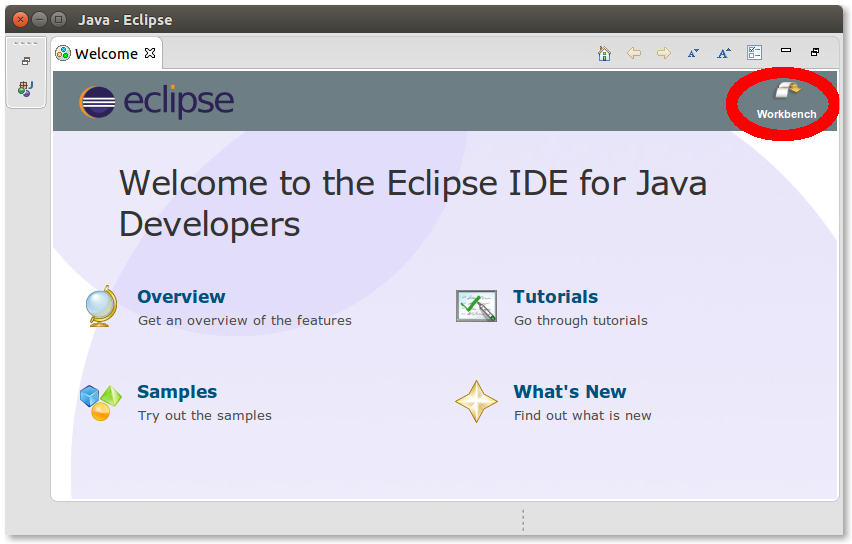
\includegraphics[width=1.0\textwidth]{../img/eclipse/eclipse-welcome.png}
\caption{Välkomstfliken för Eclipse, som nås via menyn \MenuArrow{Help}\Menu{Welcome}. Gå vidare genom att klicka på \textit{Workbench}.}
\label{fig:appendix:eclipse:welcome}
\end{figure}

\subsubsection{Välja perspektiv och visa olika vyer}

Eclipse-fönstret kan innehålla många underfönster i olika flikar, så kallade \textbf{views} eller vyer, som kan arrangeras på olika vis efter hur du vill ha dem. Vilka vyer som syns och hur de placeras beror på vilket s.k. \textbf{perspective} som är aktivt.  Figur \ref{fig:appendix:eclipse:open-perspective} visar arbetsytan med olika vyer i Java-perspektivet. 

Du kan byta till Scala-perspektivet genom att trycka på 
\includegraphics[scale=0.75]{../img/eclipse/eclipse-perspective-button.png} eller genom menyn \MenuArrow{Window}\MenuArrow{Perspective}\MenuArrow{Open Perspective}\MenuArrow{Other...}\Menu{Scala}.
Du kan anpassa inställningarna så att Scala blir \textit{default perspective}, se steg \ref{item:scala-perspective} i avsnitt \ref{subsection:appendix:ide:eclipse:tweaks} på sidan \pageref{subsection:appendix:ide:eclipse:tweaks}.

Stäng vyerna \textit{Task List} och \textit{Outline} om du vill ha mer plats till de övriga vyerna för paketnavigering, editering och utdata. Du kan öppna stängda vyer igen genom menyn \MenuArrow{Window}\Menu{Show View}. 

\begin{figure}
\centering
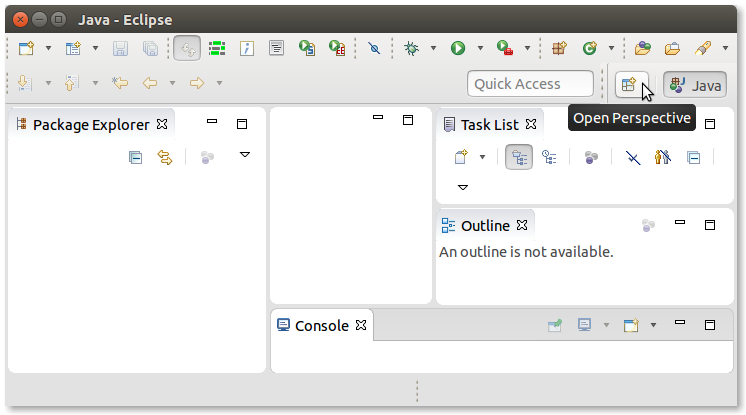
\includegraphics[width=1.0\textwidth]{../img/eclipse/eclipse-open-perspective.png}
\caption{Arbetsytan i Eclipse. Du kan växla mellan Scala- och Java-perspektivet genom att klicka på perspektivvalsknappen.}
\label{fig:appendix:eclipse:open-perspective}
\end{figure}

\subsubsection{Hello World}\label{subsubsection:eclipse:hello-world}

Efter att du öppnat Eclipse med ScalaIDE i ett tomt workspace och valt Scala-perspektivet enligt föregående avsnitt, kan du skapa ditt första projekt med ett \textit{''Hello World''}-program enligt stegen nedan.

\begin{enumerate}
\item Högerklicka i \Menu{Package Explorer} och välj \MenuArrow{New}\Menu{Scala Project}, varefter en dialogruta visas. 

\item Fyll i namnet \texttt{hello} i fältet \Menu{Project Name} och klicka \Button{Finish}.

\item Högerklicka igen i \Menu{Package Explorer} och välj \MenuArrow{New}\Menu{Scala Object}, varefter en ny dialogruta visas. 

\item Fyll i namnet \texttt{hi} i fältet \Menu{Project Name} och klicka \Button{Finish}.

\item Du får nu i editorvyn ett kodskellet med \code{object hi}.

\item Börja skriv \code{main} som visas i figur \ref{fig:appendix:eclipse:complete-main} och tryck Ctrl+Mellanslag för att aktivera kodkomplettering \Eng{code completion}. Då får du upp en lista med alternativ. Välj det översta alternativet \texttt{main} varefter ett kodskellet med en main-metod klistras in automatiskt i din kod.

\begin{figure}
\centering
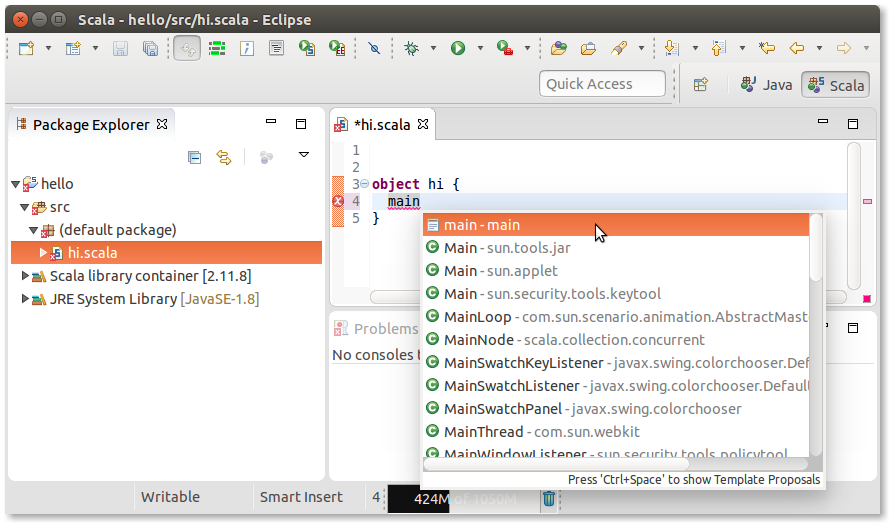
\includegraphics[width=1.0\textwidth]{../img/eclipse/eclipse-complete-main.png}
\caption{Aktivera kodkomplettering med Ctrl+Mellanslag efter ordet \code{main}.}
\label{fig:appendix:eclipse:complete-main}
\end{figure}

\item Fyll i lämplig utskriftstext i ett \code{println}-anrop så att din \code{main}-metod blir så som visas i editorfliken i figur \ref{fig:appendix:eclipse:hello-world}.

\begin{figure}[H]
\centering
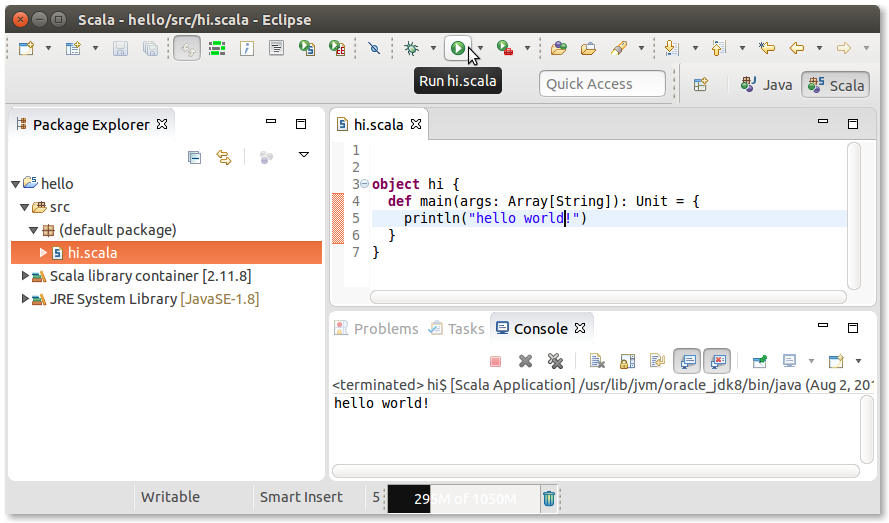
\includegraphics[width=1.0\textwidth]{../img/eclipse/eclipse-hello-world.png}
\caption{Skriv klart \code{main}-metoden och kör ditt program med play-knappen.}
\label{fig:appendix:eclipse:hello-world}
\end{figure}

\item Kör ditt program genom att trycka på den gröna play-knappen, som muspekaren i figur \ref{fig:appendix:eclipse:hello-world} pekar på. Du kan också trycka F11 för att köra igång din app, efter att du vid första körningen i dialogen \textit{Select Preferred Launcher} markerat  \FramedCheckmark{Use configuration specific settings} och valt alternativet \textit{Scala Application (new debugger) Launcher}. 

\end{enumerate}




\subsubsection{Ladda ner kursens workspace och importera projekt till labbarna}

Det finns en zip-fil med ett workspace med projekt för flera av kursens laborationer som du kan ladda ner och importera i Eclipse. Följ stegen nedan.

\begin{enumerate}
\item Ladda ner kursens workspace här: \url{http://cs.lth.se/pgk/ws}

\item Packa upp filen på lämpligt ställe.

\item Starta Eclipse med ScalaIDE-plugin (se startinstruktioner på sidan \pageref{subsubsection:start:eclipse}). 

\item Växla workspace till biblioteket du nyss packade upp, ungefär som i figur \ref{fig:eclipse:ide:open} och klicka \Button{OK}.
\begin{figure}[H]
\centering
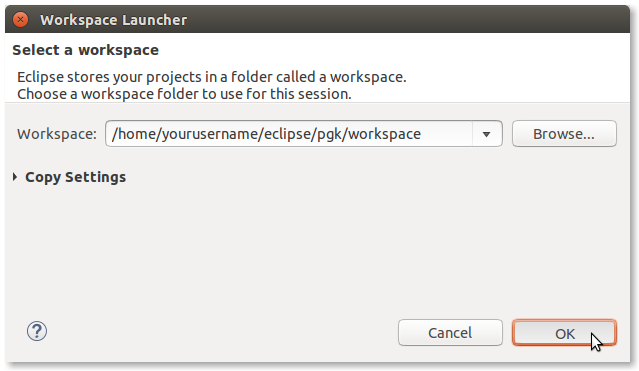
\includegraphics[width=1.0\textwidth]{../img/eclipse/eclipse-select-workspace.png}
\caption {Öppna kursens workspace genom att bläddra till biblioteket där du packade upp filen som du laddat ned från: \url{http://cs.lth.se/pgk/ws} }
\label{fig:eclipse:ide:open}
\end{figure}

\item Stäng välkomstfliken för att komma vidare till workbench (se figur \ref{fig:appendix:eclipse:welcome} på sidan \pageref{fig:appendix:eclipse:welcome}). Det ser då ut ungefär som i figur~\ref{fig:appendix:eclipse:open-perspective} på sidan \pageref{fig:appendix:eclipse:open-perspective}. Det syns ännu inget i \textit{Package Explorer} då vi ännu inte importerat något projekt. 

\item Innan du går vidare, säkerställ att du har Scala-perspektivet aktiverast. Du kan växla till Scala-perspektivet genom att trycka på 
\includegraphics[scale=0.75]{../img/eclipse/eclipse-perspective-button.png} eller genom menyn \MenuArrow{Window}\MenuArrow{Perspective}\MenuArrow{Open Perspective}\MenuArrow{Other...}\Menu{Scala}.
Du kan anpassa inställningarna så att Scala blir \textit{default perspective}, se steg \ref{item:scala-perspective} i avsnitt \ref{subsection:appendix:ide:eclipse:tweaks} på sidan \pageref{subsection:appendix:ide:eclipse:tweaks}.


\item Högerklicka i \textit{Package Explorer} och välj \Menu{Import...}, se Fig.~\ref{fig:eclipse:import}, eller välj menyn \MenuArrow{File}\Menu{Import...}. 

\begin{figure}[H]
\centering
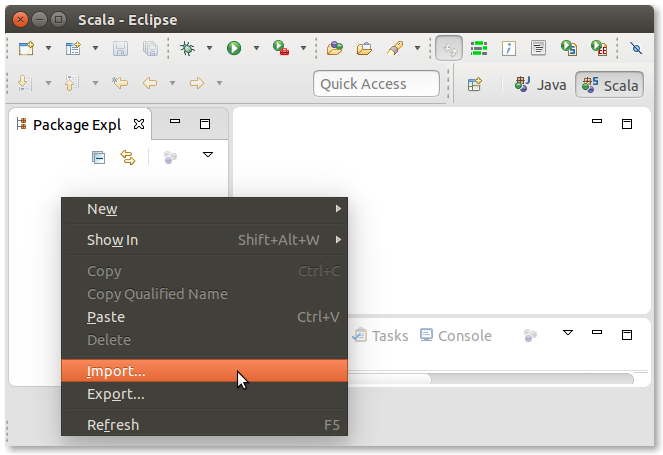
\includegraphics[width=1.0\textwidth]{../img/eclipse/eclipse-import.png} 

\caption {Välj \Menu{Import}-menyn för att importera existerande projekt.}
\label{fig:eclipse:import}
\end{figure}

\item Nu öppnas \Menu{Import}-dialogen som visas i figur \ref{fig:eclipse:import-existing}. Öppna mappen \Menu{General}, markera \textbf{Existing Projects into Workspace} och klicka \Button{Next}.



\begin{figure}[H]
\centering
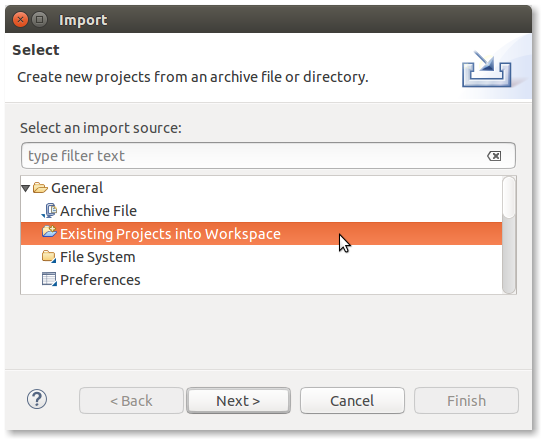
\includegraphics[width=0.75\textwidth]{../img/eclipse/eclipse-import-existing.png} 

\caption {Välj att importera existerande projekt under \Menu{General}.}
\label{fig:eclipse:import-existing}
\end{figure}


\begin{figure}[H]
\centering
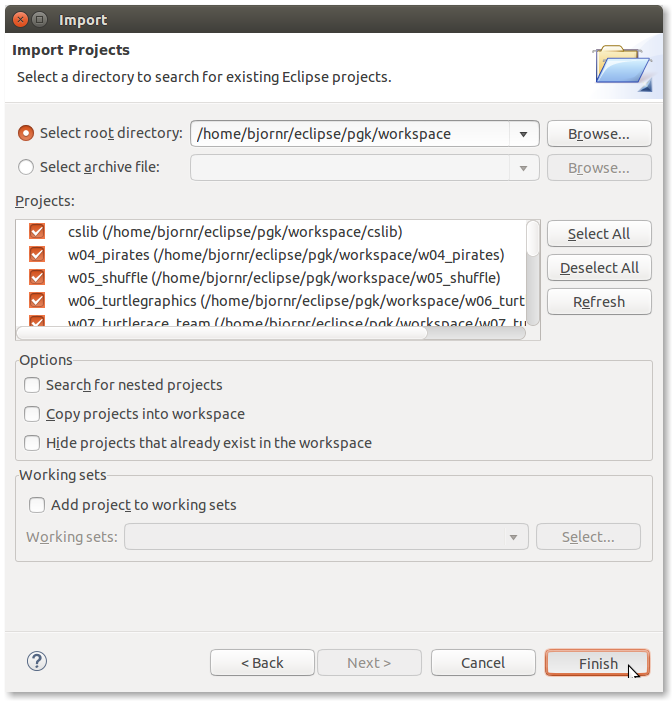
\includegraphics[width=1.0\textwidth]{../img/eclipse/eclipse-import-projects.png} 

\caption {Välj \FramedCheckmark{Select Root Directory} och klicka \Button{Browse}.}
\label{fig:eclipse:import-projects}
\end{figure}


\item Nu kommer ytterligare ett dialogfönster som visas i figure \ref{fig:eclipse:import-projects}. Med \FramedCheckmark{Select Root Directory} markerad kan du klicka \Button{Browse} för att ange workspace-mappen i ännu en dialog där du bara ska trycka \Button{Ok} utan att välja underbibliotek till workspace. När det är klart ska det se ut som i figur \ref{fig:eclipse:import-projects} där alla Eclipse-projekt \FramedCheckmark{cslib}, \FramedCheckmark{w04\_pirates}, etc. är markerade. Klicka sedan \Button{Finish}.

\item Följ ''Hello World''-instruktionerna på sidan \pageref{subsubsection:eclipse:hello-world} och skapa programmet som visas i figure \ref{fig:eclipse:pirates-hi}, genom att veckla ut projektet \textbf{w04\_pirates}, markera och högerklicka på paketet \textbf{priates}, och välja \MenuArrow{New}\Menu{Scala Object}.

\begin{figure}[H]
\centering
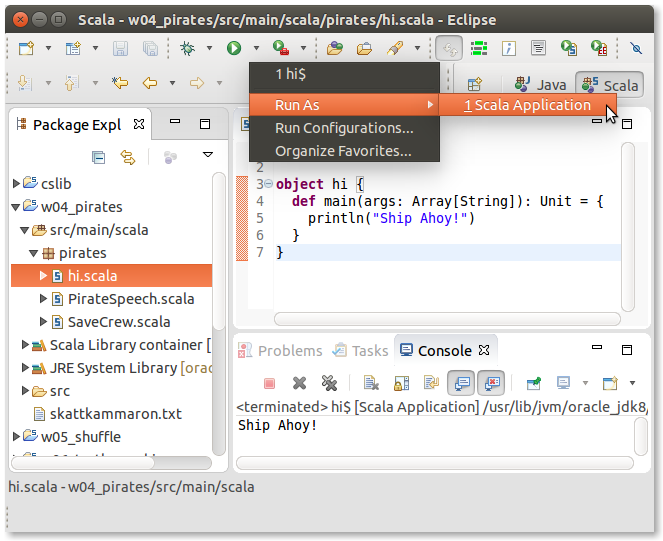
\includegraphics[width=1.0\textwidth]{../img/eclipse/eclipse-pirates-hi.png} 

\caption {Skapa ett \MenuArrow{New}\Menu{Scala Object} med kod enligt bilden.}
\label{fig:eclipse:pirates-hi}
\end{figure}


\end{enumerate}



\newpage

\section{IntelliJ IDEA}\label{appendix:ide:intellij}

IntelliJ IDEA%
\footnote{\href{https://en.wikipedia.org/wiki/IntelliJ_IDEA}{en.wikipedia.org/wiki/IntelliJ\_IDEA}}
 är en professionell IDE som stödjer många olika programmeringsspråk. IntelliJ är skriven i Java och utvecklas av det tjeckiska företaget JetBrains. 

IntelliJ IDEA finns i två varianter: en gratis gemenskapsvariant med öppenkällkodslicens \Eng{Community edition}, samt en betalvariant med stängd källkod och support-tjänster.


Till IntelliJ IDEA finns en insticksmodul \Eng{plug-in} som erbjuder stöd för Scala med tillhörande standardbibliotek..

IntelliJ IDEA är en omfattande och avancerad programmeringsmiljö med många funktioner och inställningar. Det finns även en omfattande uppsättning insticksmoduler och tilläggsprogram som underlättar utveckling av t.ex. webbprogram, databaser och mycket annat. 

I detta avsnitt ges länkar till installation samt tips om hur du kommer igång med att använda IntelliJ IDEA med Scala. Det går ganska snabbt att lära sig grunderna, men det kräven en viss ansträngning att lära sig de mer avancerade funktionerna. Det finns omfattande resurser på nätet som hjälper dig vidare. 

Google tillkännagav 2013 att företaget övergår från Eclipse till IntelliJ som den officiellt understödda utvecklingsmiljön för Android och 2014 lanserades utvecklingsmiljön AndroidStudio%
\footnote {\href{https://en.wikipedia.org/wiki/Android_Studio}{en.wikipedia.org/wiki/Android\_Studio}}
 som bygger vidare på IntelliJ. 

\subsection{Installera IntelliJ med Scala}\label{appendix:ide:intellij:install}

IntelliJ med Scala-plug-in är förinstallerat på LTH:s datorer och startas med kommandot \texttt{intellij} i ett terminalfönster.

\TODO Beskriv hur man installerar IntelliJ med Scala

\subsection{Använda IntelliJ}\label{appendix:ide:intellij:use}

\TODO 

%!TEX encoding = UTF-8 Unicode
%!TEX root = ../compendium2.tex

\chapter{Skapa webb-appar med ScalaJS}\label{appendix:scalajs}

\begin{itemize}
\item Lär mer här: \url{http://scala-js.org/}
\item Exempel: \url{https://github.com/bjornregnell/kapten-alloc-web}
\item Exempel på konfiguration av bygge:
\begin{itemize}
\item Lägg in plugin för ScalaJS i \texttt{project/plugins.sbt}: \\\url{https://github.com/bjornregnell/kapten-alloc-web/blob/master/project/plugins.sbt}
\item Lägg till ScalaJS-biblioteket i \texttt{build.sbt}: \\\url{https://github.com/bjornregnell/kapten-alloc-web/blob/master/build.sbt} 
\item Lägg till \texttt{<script>}-tag i \code{index.html}: \\\url{https://github.com/bjornregnell/kapten-alloc-web/blob/master/index.html} 
\item Skapa webbappen med \code{sbt fastLinkJS} vid utveckling och när klar så skapa optimerad app med \code{sbt fullLinkJS}
\end{itemize}
\end{itemize}
%!TEX encoding = UTF-8 Unicode
%!TEX root = ../compendium2.tex

\chapter{Skapa Android-appar i Scala}\label{appendix:scala-android}

\TODO

\noindent Läs först appendix \ref{appendix:build}

\begin{itemize}
\item \url{http://scala-android.org/}
\end{itemize}

\part{Lösningar}

\setcounter{chapter}{11} %next is L in \Alph
\chapter{Lösningar till övningarna}\label{chapter:solutions}
\setcounter{section}{7}

\PreSolutionfalse
%!TEX encoding = UTF-8 Unicode

%!TEX root = ../solutions.tex

\ExerciseSolution{\ExeWeekEIGHT}

\BasicTasks %%%%%%%%%%%

%Uppgift 1
\Task

%1.a)
\Subtask  
\includegraphics{../img/w09-solutions/1a} \\
Typ: \code{Vector[Vector[Int]]}\\
Värde: \code{Vector(Vector(1, 2, 3, 4, 5), Vector(3, 4, 5, 6, 7))} \\
Dimensioner: $2 \times 5$\\
Inom matematiken sker indexering enligt konvention med 1 som lägsta index. I scala är lägsta index 0, man använder s.k. 0-indexering. \footnote{Detta är inte fallet i alla programmeringsspråk, vilket du kan läsa mer om på \url{https://en.wikipedia.org/wiki/Array\_data\_type\#Index\_origin}}

%1. b)
\Subtask \\
2: \code{Int}\\
3: \code{Vector[Int]}\\
4: \code{Int}

%1.c)
\Subtask \\
m2: \code{Vector[Vector[Int]]}\\
m3: \code{Vector[Vector[AnyVal]]}\\
m4: \code{Vector[Vector[Any]]}\\
m5: \code{Vector[Vector[Int]]}

%1.d)
\Subtask TODO

%1.e)
\Subtask m5, $42 \times 2$

%Uppgift 2
\Task

%2.a)
\Subtask \begin{Code}
def throwDie: Int = (math.random * 6).toInt + 1
\end{Code}

%2.b)
\Subtask $1000 \times 5$

%2.c)
\Subtask -- %Inget svar

%2.d)
\Subtask \begin{Code}
def roll(n: Int) = Vector.fill(n)(throwDie).sorted
\end{Code}

%2.e)
\Subtask \begin{Code}
def isYatzy(xs: Vector[Int]): Boolean = xs.forall(_ == xs(0))
\end{Code}

%2.f)
\Subtask \begin{Code}
def isYatzy(xs: Vector[Int]): Boolean = {
	var foundDiff = false
	var i = 0
	while (i < xs.size && !foundDiff) {
		foundDiff = xs(i) != xs(0)
		i += 1
	}
	!foundDiff
}
\end{Code}

%2.g)
\Subtask \begin{Code}
def diceMatrix(m: Int, n: Int): Vector[Vector[Int]] =
  Vector.fill(m)(roll(n))
\end{Code}

%2.h)
\Subtask \begin{Code}
def diceMatrixToString(xss: Vector[Vector[Int]]): String =
  xss.map(_.mkString(" ")).mkString("\n")
\end{Code}

%2.i)
\Subtask Funktionen går igenom varje matrisrad, där den i sin tur går igenom
varje element på raden och lägger till i \code{StringBuilder}-objektet. Om det inte är
det sista elementet på raden läggs även ett blanktecken till, annars läggs ett
nyradstecken till. Undantaget är sista raden, där inget nyradstecken läggs till.
Slutligen konverteras \code{StringBuilder}-objektet till en \code{String} som
returneras.\\
Är \code{xss} tom utvärderas \code{0 until xss.size} till en tom \code{Range}
eftersom \code{xss.size} blir \code{0} och \code{until} är exkluderande.
Innehållet i den yttre \code{for}-loopen hoppas över och en tom sträng returneras.
Är alla rader tomma hoppas i stället de inre \code{for}-looparna över, med samma resultat.\\
Med \code{StringBuilder} behöver inte hela innehållet kopieras vid varje tillägg,
vilket spar prestanda vid många tillägg,
men eftersom det är ett föränderligt objekt kan innehållet ändras av någon annan
del av programmet som också har tillgång till referensen; objektet kan helt plötsligt
 innehålla någonting annat, trots att referensen är densamma.

%2.j)
\Subtask \begin{Code}
def filterYatzy(xss: Vector[Vector[Int]]): Vector[Vector[Int]] =
  xss.filter(isYatzy)
\end{Code}

%2.k)
\Subtask \begin{CodeSmall}
def filterYatzy(xss: Vector[Vector[Int]]): Vector[Vector[Int]] = {
	var result: Vector[Vector[Int]] = Vector()
	for (i <- 0 until xss.size) {
		if (isYatzy(xss(i))) result = result :+ xss(i)
	}
	result
}
\end{CodeSmall}

%2.l)
\Subtask --

%2.m)
\Subtask \begin{Code}
def yatzyPips(xss: Vector[Vector[Int]]): Vector[Int] =
  xss.filter(isYatzy).map(_.head)
\end{Code}


%Uppgift 3
\Task     %starts with: \emph{Strängtabell med rubrikra%%%

%3.a)
\Subtask \begin{CodeSmall}
case class Table(
	data: Vector[Vector[String]],
	headings: Vector[String],
	sep: String){

	val dim: (Int, Int) = (data.size, headings.size)

	def apply(r: Int, c: Int): String = data(r)(c)

	def row(r: Int): Vector[String]= data(r)

	def col(c: Int): Vector[String] = data.map(r => r(c))

	lazy val indexOfHeading: Map[String, Int] = headings.zipWithIndex.toMap

	def col(h: String): Vector[String] = col(indexOfHeading(h))

	def values(h: String): Vector[String] = col(h).distinct.sorted

	override lazy val toString: String =
		headings.mkString(sep) + "\n" +data.map(_.mkString(sep)).mkString("\n")
}
object Table {
	def fromFile(fileName: String, separator: Char = ';'): Table = {
		val lines = scala.io.Source.fromFile(fileName).getLines.toVector
		val matrix= lines.map(_.split(separator).toVector)
		new Table(matrix.tail, matrix.head, separator.toString)
	}
}
\end{CodeSmall}

%3.b)
\Subtask \begin{CodeSmall}
object RegTable {
 	def main( args:Array[String]): Unit = {
		val t = Table.fromFile(args(0), args(1)(1))
		val counts: Vector[Vector[String]] =
 			(0 until t.dim._2)
				.map(i => t.values(t.headings(i))
				.map(x => x + ": " + t.col(i).count(_ == x)))
				.toVector

    for (i <- 0 until t.dim._2) {
      println(s"\nColumn: ${i + 1}, ${t.headings(i)}:")
      for (j <- 0 until counts(i).length) {
        println(counts(i)(j))
      }
    }
  }
}
\end{CodeSmall}

%Uppgift 4
\Task     %starts with: \emph{Generiska funkioner.} En %%%

%4.a)
\Subtask  \begin{enumerate}
\item --
\item Strängrepresentationen av \code{42} spegelvänds
\item \code{"hej"} spegelvänds - \code{toString} av en sträng ger en likadan sträng
\item --
\item Gurk-objektets strängrepresentation spegelvänds
\item Funktionens typparameter matchar inte parameterns typ: \code{42} är ingen sträng
\item Implicit typkonvertering till \code{Double} sker för att stämma överens med typparametern, vilket ger en strängrepresentation med decimal
\end{enumerate}

%4.b)
\Subtask  \begin{enumerate}
\item En funktion definieras så att den tar emot två andra funktioner som argument, sätter ihop dem, och matar in ett tredje argument till den den sammansatta funktionen
\item En funktion som inkrementerar ett heltal med 1 definieras
\item En funktion som halverar ett flyttal definieras
\item \code{42} matas in i \code{inc()} och resultatet (\code{43}) matas vidare till \code{half()}. Inuti \code{half()} sker implicit typkonvertering till \code{Double} då talet divideras med ett flyttal (\code{2.0}) och resultatet blir \code{43.0 / 2.0}, alltså \code{21.5}.
\item Resultatet från \code{half()} är av typ \code{Double}, medan \code{inc()} tar emot ett argument av typ \code{Int}. Då flyttal generellt inte kan konverteras till heltal utan informationsförlust sker ingen implicit konvertering, istället sker ett kompileringsfel.
\end{enumerate}

%4.c)
\Subtask \begin{Code}
def inc(x: Double): Double = x + 1.0
\end{Code}
Nu ges kompileringsfel på rad 4 istället, vilket kan lösas med följande ändring:
\begin{Code}
def half(x: Double): Double = x / 2.0
\end{Code}


%Uppgift 4
\Task     %starts with: \emph{Generiska klasser.} Även %%%

%5.a)
\Subtask --

%5.b)
\Subtask \begin{Code}
class Cell[T](var value: T){
	override def toString = "Cell(" + value + ")"
	def concat[U](that: Cell[U]): Cell[String] =
		new Cell(value.toString + that.value.toString)
}
\end{Code}

%5.c)
\Subtask  Endast celler med samma typparameter kan nu konkateneras. Eftersom \code{concat()} returnerar ett objekt av typ \code{Cell[String]} kan ett ojämnt antal celler med någon annan typparameter än \code{String} alltså inte längre konkateneras. Är antalet jämnt går det att konkatenera dem parvis och sedan konkatenera de returnerade \code{Cell[String]}-objekten, men det är något omständigt.

%5.d)
\Subtask  --


%Uppgift 6
\Task     %starts with: \label{task:arraymatrix-java} \%%%

%6.a)
\Subtask Vid initialisering fylls alla element i \code{xss} med standardvärdet för typen, \code{0} i fallet med \code{int}. Den yttre \code{for}-loopen i \code{showMatrix()} itererar över raderna i \code{xss}. Den inre \code{for}-loopen itererar i sin tur längs med elementen på den auktuella raden och skriver ut rad, kolumn och innehåll. Efter varje rad sker en radbrytning, så att en rad i utskriften även motsvarar en rad i matrisen.\\
Exempel på skillnader mellan användning av matriser i scala och java:
\begin{itemize}
\item åtkomst: \code{minArray(rad)(kolumn)} respektive \code{minArray[rad][kolumn]}
\item typnamn: \code{Array[Array[elementTyp]]} respektive  \code{elementTyp[][]}
\item allokering: \code{Array.ofDim[typ](xDim,yDim)} respektive \code{new typ[xDim][yDim]}
\end{itemize}

%6.b)
\Subtask \begin{Code}
public class ArrayMatrix {

	public static void showMatrix(int[][] m){
		System.out.println("\n--- showMatrix ---");
		for (int row = 0; row < m.length; row++){
			for (int col = 0; col < m[row].length; col++) {
				System.out.print("[" + row + "]");
				System.out.print("[" + col + "] = ");
				System.out.print(m[row][col] + ";");
			} System.out.println();
		}
	}

	public static void fillRnd(int[][] m, int n){
		for (int row = 0; row < m.length; row++){
			for (int col = 0; col < m[row].length; col++) {
				m[row][col] = (int) (Math.random() * n + 1);
			}
		}
	}

	public static void main(String[] args) {
		System.out.println("ArrayMatrix test");
		int[][] xss = new int[10][5];
		showMatrix(xss);
		fillRnd(xss, 6);
		showMatrix(xss);
	}
}
\end{Code}

\ExtraTasks %%%%%%%%%%%%

%Uppgift 7
\Task     %starts with: \emph{Skapa ett yatzy-spel för %%%

%7.a)
\Subtask  \begin{CodeSmall}
/** En skiss på en klass som kan användas till ett förenklat yatzy-spel */
case class YatzyRows(val rows: Vector[Vector[Int]]) {

	private def throwDie: Int = (math.random * 6).toInt + 1

	/** A new YatzyRows with a new row of 5 dice rolls appended to rows */
	def roll: YatzyRows = new YatzyRows(rows :+ Vector.fill(5)(throwDie))

	/** A new YatzyRow with some indices of the last row re-rolled */
	def reroll(indices: Vector[Int]): YatzyRows =
		new YatzyRows(rows :+ rows(rows.length - 1).zipWithIndex.map {
			case (x, i) => if (indices.contains(i)) throwDie else x
		})
}
object YatzyRows {

	def isYatzy(xs: Vector[Int]): Boolean = xs.forall(_ == xs(0))

	def isThreeOfAKind(xs: Vector[Int]): Boolean =
		xs.exists(x => xs.count(_ == x) >= 3)

	def isFourOfAKind(xs: Vector[Int]): Boolean =
		xs.exists(x => xs.count(_ == x) >= 4)

	def isFullHouse(xs: Vector[Int]): Boolean =
		xs.exists(x => xs.count(_ == x) == 3) &&
		xs.exists(x => xs.count(_ == x) == 2)

	def isSmallStraight(xs: Vector[Int]): Boolean =
		xs.forall(x => xs.count(_ == x) == 1) && !xs.exists(_ == 6)

	def isLargeStraight(xs: Vector[Int]): Boolean =
		xs.forall(x => xs.count(_ == x) == 1) && !xs.exists(_ == 1)
}

\end{CodeSmall}
Observera att fem stycken 2:or uppfyller kraven för Yatzy, men även för triss och fyrtal.

\Subtask  Slumpen gör att utfallet inte kommer stämma exakt överens med teorin, men för ett stort antal kast bör resultaten hamna ganska nära. De teoretiska sannolikheterna (utan omkast) finns i \ref{yatzyProb}.
\begin{table}[h]
\centering
\caption{Sannolikhet för olika Yatzy-resultat}
\label{yatzyProb}
\begin{tabular}{ll}
Yatzy&  $0,077\%$  \\
$\geq3$ av samma& $21\%$\\
$\geq4$ av samma& $2,0\%$\\
Kåk& $3,9\%$\\
Liten stege& $1,5\%$\\
Stor stege& $1,5\%$
\end{tabular}
\end{table}

Kodexempel:
\begin{CodeSmall}
import YatzyRows._

object YatzyStats extends App {
  val n = 1000000.0
  var yr = YatzyRows(Vector(Vector[Int]()))
  for (i <- 1 to n.toInt) yr = yr.roll
  println(s"Yatzy: ${yr.rows.count(isYatzy(_)) / n * 100}%")
  println(s"Three of a kind: ${yr.rows.count(isThreeOfAKind(_)) / n * 100}%")
  println(s"Four of a kind: ${yr.rows.count(isFourOfAKind(_)) / n * 100}%")
  println(s"Full house: ${yr.rows.count(isFullHouse(_)) / n * 100}%")
  println(s"Small straight: ${yr.rows.count(isSmallStraight(_)) / n * 100}%")
  println(s"Large straight: ${yr.rows.count(isLargeStraight(_)) / n * 100}%")
}
\end{CodeSmall}

\Subtask --

\AdvancedTasks %%%%%%%%%

\Task     %%%TODO number  8 %%%starts with: \label{task:generic-matrix} \em%%%

\Subtask -- %%%TODO in task 8 %%%


\Task     %%%TODO number  9 %%%starts with: \TODO \emph{Klasser för täta oc%%%

\Subtask -- %%%TODO in task 9 %%%

\Subtask -- %%%TODO in task 9 %%%

\Subtask -- %%%TODO in task 9 %%%

\Subtask -- %%%TODO in task 9 %%%

\Subtask -- %%%TODO in task 9 %%%

\Subtask -- %%%TODO in task 9 %%%


\Task     %%%TODO number  10 %%%starts with: \emph{Matriser med \jcode{Array%%%

\Subtask -- %%%TODO in task 10 %%%

%!TEX encoding = UTF-8 Unicode

%!TEX root = ../solutions.tex

\ExerciseSolution{\ExeWeekNINE}

\BasicTasks %%%%%%%%%%%

\Task

\Subtask \code{Vector[Object]}.

\Subtask Det beror på att vektorns element är av typen \code{Object}. \code{vikt} är inte definierat för denna typ.

\Subtask -.

\Subtask \code{Vector[Grönsak]}.

\Subtask Ja.

\Subtask -.

\Subtask \code{Grönsak}. \$anon\$1@88dfbe.

\Task

\Subtask
\begin{Code}
def skapaDjur: Djur =
   {if(math.random > 0.5) new Ko else new Gris}
\end{Code}

\Subtask
\begin{Code}
class Häst extends Djur{ def väsnas = println("Gnääääägg") }
def skapaDjur: Djur = {val r = math.random;
   if(r < 0.33) new Ko else if(r < 0.67) new Gris else new Häst}
\end{Code}

\Task

\Subtask
\begin{Code}
val c1 = Circle(Point(1, 1), 42)
val r1 = Rectangle(Point(3, 3), 20, 30)
c1.move(2, 3)
r1.move(3, 2)
\end{Code}

\Subtask För \code{Point}: \code{def moveTo(dx: Double, dy: Double): Point = Point(dx, dy)}. \\
För \code{Shape}: \code{def moveTo(dx: Double, dy: Double): Shape}. \\
För \code{Rectangle}: \code{override def moveTo(dx: Double, dy: Double): Rectangle = } \\
\code{Rectangle(pos.moveTo(dx, dy), this.dx, this.dy)}. \\
För \code{Circle}: \code{override def moveTo(dx: Double, dy: Double): Circle =} \\
\code{Circle(pos.moveTo(dx, dy), radius)}.

\Subtask \code{def distanceTo(that: Point): Double = math.hypot(that.x - x, that.y - y)}.

\Subtask \code{def distanceTo(that: Shape): Double = pos.distanceTo(that.pos)}.

\Task

\Subtask
\begin{Code}
fyle.filter(f => f.isInstanceOf[Ånka] && f.ärFlygkunnig).size
\end{Code}

\Subtask
\begin{Code}
val antalKrax: Int = fyle.filter(f => !f.ärSimkunnig).size * 2
val antalKvack: Int = fyle.filter(f => f.ärSimkunnig).size * 4
\end{Code}

\Task

\Subtask Sätt \code{final} framför \code{class} i klasserna.

\Subtask error: illegal inheritance from final class Kråga.

\Task

\Subtask error: not found: value minHemlis.

\Subtask error: value vårHemlis in class Super\$class cannot be accessed in Sub.

\Subtask Ja.

\Task

\Subtask I Fyle:
\begin{Code}
protected var räknaLäte: Int = 0
def väsnas: Unit = { print(läte * 2); räknaLäte += 2 }
\end{Code}

I Ånka: \code| override def väsnas = { print(läte * 4); räknaLäte += 4 }|

\Subtask \code{ def antalLäten: Int = räknaLäte }

\Subtask Om en klass som representerar en fågel som skulle ge ifrån sig fler/färre läten än en vanlig \code{Fyle}, behöver \code{väsnas} ändras. Denna metod behöver tillgång till \code{räknaLäte}, vilken inte får vara \code{private}.

\Subtask Räknar-variabeln ska inte kunna påverkas i någon annan del av programmet.

\Task

\Subtask B ärver A. C och D ärver B.

\Subtask 1. True eftersom c är av typen C. \\
2. False eftersom c inte är av typen D. \\
3. True eftersom d är av typen D som är en subtyp av B. \\
4. True eftersom c är av typen C som är en subtyp av B, som i sin tur är en subtyp av A. \\
5. True eftersom b är av typen D, som är en subtyp av B, som i sin tur är en subtyp av A. \\
6. True eftersom b är av typen D. \\
7. True eftersom a är av typen C som är en subtyp av B. \\
8. True eftersom c är av typen C som är en subtyp av AnyRef. \\
9. True eftersom c är av typen C som är en subtyp av Any. \\
10. Error eftersom \code{isInstanceOf} inte kan använda sig av \code{AnyVal}.  \\
11. True eftersom c är av typen C som är en subtyp av Object (Object är java-representationen av AnyRef). \\
12. Error eftersom \code{isInstanceOf} inte kan testa om värdetyper (i detta fallet \code{42}) är referenstyper. \\
13. True eftersom \code{42} är av typen \code{Int} som är en subtyp av Any. \\

\Subtask 3. Går inte eftersom c inte är av typen D, utan typen C. \\
6. Går inte eftersom a inte är av typen D, utan typen C. \\
7. Går inte eftersom typen E inte finns. \\

\Task

\Subtask 2. Måste ha \code{override} framför \code{b} för att kunna ändra på metoden. \\
4. \code{c} är \code{private}, vilket betyder att den är gömd för subklasserna. Därför kan den inte överskuggas. Genom att ta bort \code{override} fungerar klassen. \\
5. En \code{final}-medlem måste ha ett bestämt värde. Kan lösas genom att tilldela \code{final a} ett värde eller ta bort \code{final}. \\
6. En \code{final}-medlem kan inte överskuggas, varken med eller utan \code{override}. Här får konflikterna tas bort.  \\
7. Se 6. \\
8. Eftersom \code{c} inte finns i \code{Super5} kan den inte överskuggas. Genom att ta bort \code{override} fungerar klassen. \\
10. Överskuggningen av \code{val} måste vara oföränderlig (immutable); detta är inte nödvändigtvis \code{def}. Löses genom att byta ut \code{def a} mot \code{val a} hos \code{Sub10}.  \\
11. Samma problem som i 10.; \code{lazy val} kan vara föränderlig. Löses genom att ta bort \code{lazy}. \\
12. Samma problem igen! \code{var} är föränderlig, vilket bryter mot typsäkerheten när man försöker överskugga en \code{val}. Löses genom att ändra \code{var} till \code{val}. \\
15.\code{def a = 43} och \code{val c = "?"} täcker inte allt som \code{var} kräver. Det behövs en setter för att kunna uppfylla kraven för överskuggning för en \code{var}. Dessutom finns det ingen anledning för en \code{val} att överskuggas; man kan ju ändra på den lite hur man vill!

\Subtask Sub3: a = 43, b = 43 eftersom medlemmen är överskuggad. c hittas inte eftersom den är \code{private}.

Sub13: a = 43, b = 42, c = "still lazy" eftersom medlemmen överskuggas.

SubSub: a = 44 eftersom medlemmen överskuggas, b = 42, c = "still lazy".

\Subtask -.

\Task

\Subtask
\begin{Code}
val person = new Person("Person1")
val akademiker = new Akademiker("Person2", "LTH")
val student = new Student("Person3", "LTH", "D")
val forskare = new Forskare("Person4", "LTH", "Doktorand")
\end{Code}

\Subtask
\begin{Code}
val vec = Vector(person, akademiker, student, forskare)
for(i <- vec){ print(i.toString + i.namn) }
\end{Code}

\Subtask error: class Person is abstract; cannot be instantiated.

\Subtask error: overriding value namn in class Person of type String; value namn needs `override' modifier.\\
toString för Student: Student(Person3,LTH,D). \\
toString för Forskare: Student(Person4,LTH,Doktorand).

\Subtask
\begin{Code}
trait Person {val namn: String; val nbr: Int}
trait Akademiker extends Person {val universitet: String}
case class Student(
  namn: String,
  nbr: Int,
  universitet: String,
  program: String) extends Akademiker
case class Forskare(
  namn: String,
  nbr: Int,
  universitet: String,
  titel: String) extends Akademiker
case class IckeAkademiker(
    namn: String,
    nbr: Int) extends Person
\end{Code}

\Subtask Man måste använda en klass om man behöver klassparametrar. Man måste använda en trait om man vill göra in-mixning med \code{with}. \\
 Se \href{http://www.artima.com/pins1ed/traits.html\#12.7}{http://www.artima.com/pins1ed/traits.html\#12.7}.

\Task

\Subtask Sättet är säkrare då man inte kan tilldela korten en färg som inte finns. Med heltalskonstanterna kan man till exempel ge ett kort färgen 5, vilken inte korresponderar till någon riktig färg.

\Subtask \code{for (f <- Färg.values; v <- 1 to 13) yield Kort(f,v)}

\Subtask
\begin{Code}
def blandadKortlek: Vector[Kort] = {
  val kortlek =
    for (f <- Färg.values; v <- 1 to 13) yield Kort(f,v)
  scala.util.Random.shuffle(kortlek)
}
\end{Code}

\Subtask \code{def färgPoäng(xs: Vector[Kort]): Int = xs.map(_.färg.toInt).sum}

\ExtraTasks %%%%%%%%%%%%

\Task

\begin{Code}
trait Fyle {
  val läte: String
  def väsnas: Unit = { print(läte * 2); räknaLäte += 2 }
  protected var räknaLäte: Int = 0
  val ärSimkunnig: Boolean
  val ärFlygkunnig: Boolean
  val ärStor : Boolean
  def antalLäten: Int = räknaLäte
}
trait KanSimma { val ärSimkunnig = true }
trait KanInteSimma { val ärSimkunnig = false }
trait KanFlyga { val ärFlygkunnig = true }
trait KanKanskeFlyga { val ärFlygkunnig = math.random < 0.8 }
trait KanKanskeSimma { val ärSimkunnig = math.random < 0.2 }
trait ÄrStor { val ärStor = true }
trait ÄrLiten { val ärStor = false }

final class Kråga
  extends Fyle
  with KanFlyga
  with KanInteSimma
  with ÄrStor{
  val läte = "krax"
}

final class Ånka
  extends Fyle
  with KanSimma
  with KanKanskeFlyga
  with ÄrStor{
  val läte = "kvack"
  override def väsnas = { print(läte * 4); räknaLäte += 4 }
}

final class Pjodd
  extends Fyle
  with KanFlyga
  with KanKanskeSimma
  with ÄrLiten{
  val läte = "kvitter"
  override def väsnas = { print(läte * 8); räknaLäte += 8 }
}
\end{Code}

I REPL:
\begin{REPL}
val fyle = Vector.fill(42)(
  if(math.random < 0.33) new Kråga else
  if (math.random < 0.5) new Ånka else
  new Pjodd)
fyle.filter(f => f.isInstanceOf[Kråga]).size*2
fyle.filter(f => f.isInstanceOf[Ånka]).size*4
fyle.filter(f => f.isInstanceOf[Pjodd]).size*8
\end{REPL}

\AdvancedTasks %%%%%%%%%

%!TEX encoding = UTF-8 Unicode

%!TEX root = ../solutions.tex

\ExerciseSolution{\ExeWeekTEN}

\BasicTasks %%%%%%%%%%%

\Task

\Subtask Beroende på första bokstaven i din favoritgrönsak får du olika svar såsom \textit{gurka är gott!} vid första bokstaven $g$.\\
Javas \jcode{switch}-sats testar den första bokstaven på favoritgrönsaken genom att stegvis jämföra den med \jcode{case}-uttrycken. Om första bokstaven \jcode{firstChar} matchar bokstaven efter ett \jcode{case} körs koden efter kolonet till \jcode{switch}-satsens slut eller tills ett \jcode{break} avbryter \jcode{switch}-satsen.\\
Matchar inte \jcode{firstChar} något \jcode{case} så finns även \jcode{default}, som körs oavsett vilken första bokstaven är, ett generellt fall.

\Subtask Om \jcode{case 't'} körs kommer både  \textit{tomat är gott!} och \textit{broccoli är gott!} skrivas ut, man säger att koden $"$faller igenom$"$. Utan \jcode{break}-satsen i Java körs koden i efterkommande \jcode{case} tills ett \jcode{break} avbryter exekveringen eller \jcode{switch}-satsen tar slut.


\Task

\Subtask Svaret blir identiskt mot föregående uppgiften i Java.\\
Scalas \code{match}-uttryck fungerar väldigt likt Javas \jcode{switch}. Den jämför stegvis värdet med varje \code{case} för att sedan returnera ett värde tillhörande motsvarande \code{case}.

\Subtask \begin{REPL}
scala.MatchError (of class java.lang.Character)
\end{REPL}
Exekveringsfel, uppstår av en viss input under körningen.

\Subtask Scalas \code{match} ersätter kolonet (:) i \jcode{switch} med Scalas högerpil (=>).\\
\code{match} returnerar ett värde till skillnad från \jcode{switch} som inte returnerar något.\\
\code{match} kan inte $"$falla igenom$"$ så ett \jcode{break} efter varje \jcode{case} är inte nödvändigt.\\
Till skillnad från \jcode{switch}-satsen kastar \code{match} ett \code{MatchError} om ingen matchning skulle ske.


\Task
\\
Garden som införts vid \code{case 'g'} slumpar fram ett tal mellan 0 och 1 och om talet inte är större än $0.5$ så blir det ingen matchning med \code{case 'g'} och programmet testar vidare tills default-caset.\\
Gardens krav måste uppfyllas för att det ska matcha som vanligt.


\Task

\Subtask G100true. Vid byte av plats: Gtrue100.\\
\code{match} testar om kompanjonsobjektet \code{Gurka} är av typen \code{Gurka} med två parametervärden. De angivna parametrarna tilldelas namn, \code{vikt} får namnet \code{v} och \code{ärRutten} namnet \code{rutten} och skrivs sedan ut. Byts namnen dessa ges skrivs de ut i den omvända ordningen.

\Subtask \code{Option[(Int, Boolean)]}

\Subtask \code{Some((100, true))}, en \code{Option} med en tupel av parametrarna från g.

\Subtask \code{ärÄtvärd} testar om \code{Grönsak g} är av typen \code{Gurka(v, rutten)} eller \code{Tomat}. Dessa har sedan garder.\\ \code{Gurka} måste ha \code{vikt} över 100 och \code{ärRutten} vara \code{false} för att \code{case Gurka} ska returnera \code{true}.\\
\code{Tomat} måste ha \code{vikt} över 50 och \code{ärRutten} vara \code{false} för att \code{case Tomat} ska returnera \code{true}.\\
Matchas inte \code{Grönsak g} med någon av dessa returneras default-värdet \code{false}.


\Task

\Subtask
\begin{Code}
package vegopoly

trait Grönsak {
	def vikt: Int
	def ärRutten: Boolean
	def ärÄtbar: Boolean
}

case class Gurka(vikt: Int, ärRutten: Boolean) extends
	Grönsak { val ärÄtbar: Boolean = (!ärRutten && vikt > 100)}
case class Tomat(vikt: Int, ärRutten: Boolean) extends
	Grönsak { val ärÄtbar: Boolean = (!ärRutten && vikt > 50)}

object Main{
	def slumpvikt: Int = (math.random*500 + 100).toInt
	def slumprutten: Boolean = math.random > 0.8
	def slumpgurka: Gurka = Gurka(slumpvikt, slumprutten)
	def slumptomat: Tomat = Tomat(slumpvikt, slumprutten)
	def slumpgrönsak: Grönsak = if (math.random > 0.2) slumpgurka
		else slumptomat

	def main(args: Array[String]): Unit = {
		val skörd = Vector.fill(args(0).toInt)(slumpgrönsak)
		val ätvärda = skörd.filter(_.ärÄtbar)
		println("Antal skördade grönsaker: " + skörd.size)
		println("Antal ätvärda grönsaker: " + ätvärda.size)
	}
}
\end{Code}

\Subtask
Följande \code{case class} läggs till:
\begin{Code}
case class Broccoli(vikt: Int, ärRutten: Boolean)
    extends Grönsak {
  val ärÄtbar: Boolean = (!ärRutten && vikt > 80)
}
\end{Code}
~\\
Därefter läggs följande till i \code{object Main} innan \code{def slumpgrönsak}:

\begin{Code}
def slumpbroccoli: Broccoli = Broccoli(slumpvikt, slumprutten)
\end{Code}
~\\
Slutligen ändras \code{def slumpgrönsak} till följande:

\begin{Code}
def slumpgrönsak: Grönsak = {    // välj t.ex. denna fördelning:
  val rnd = math.random
  if (rnd > 0.5) slumpgurka      // 50% sannolikhet för gurka
  else if (rnd > 0.2) slumptomat // 30% sannolikhet för tomat
  else slumpbroccoli             // 20% sannolikhet för broccoli
}
\end{Code}

\Subtask Fördelarna med \code{match}-versionen, och mönstermatchning i sig, är att det är väldigt lätt att göra ändringar på hur matchningen sker. Detta innebär att det skulle vara väldigt lätt att ändra definitionen för ätbarheten. Skulle dock dessa inte ändras ofta utan snarare grönsaksutbudet så kan det polyformistiska alternativet vara att föredra. Detta eftersom det skulle implementeras och ändras lättare än mönstermatchningen vid byte av grönsaker.


\Task

\Subtask
\begin{Code}
def parafärg(f: Färg): Färg = f match {
  case Spader  => Klöver
  case Hjärter => Ruter
  case Ruter   => Hjärter
  case Klöver  => Spader
}
\end{Code}

\Subtask
\begin{REPL}
<console>:17: warning: match may not be exhaustive.
It would fail on the following input: Ruter
\end{REPL}
Varningen kommer redan vid kompilering.

\Subtask
\begin{REPL}
scala.MatchError: Ruter (of class Ruter$)
  at .parafärg(<console>:17)
\end{REPL}
Detta är ett körtidsfel.

\Subtask Om en klass är \code{sealed} innebär det att om ett element ska matchas och är en subtyp av denna klass så ger Scala varning redan vid kompilering om det finns en risk för ett \code{MatchError}, alltså om \code{match}-uttrycket inte är uttömmande och det finns fall som inte täcks av ett \code{case}.\\
En förseglad supertyp innebär att programmeraren redan vid kompileringstid får en varning om ett fall inte täcks och i sånt fall vilket av undertyperna, liksom annan hjälp av kompilatorn. Detta kräver dock att alla subtyperna delar samma fil som den förseglade klassen.


\Task

\Subtask Både \code{str} och \code{vadsomhelst} matchar med inputen, oavsett vad denna är på grund av att de har en liten begynnelsebokstav.\\
 \code{str} har dock en gard att strängen måste börja med $g$ vilket gör så endast \code{val g = "gurka"} matchar med denna. \code{val x = "urka"} plockas dock upp av \code{vadsomhelst} som är utan gard.

\Subtask
\begin{REPL}
<console>:16: warning: patterns after a variable pattern cannot match (SLS 8.1
.1)
\end{REPL}
och
\begin{REPL}
<console>:17: warning: unreachable code due to variable patter 'tomat' on line
16
\end{REPL}
Trots att en klass \code{tomat} existerar så tolkar Scalas \code{match} den som en \code{case}-gren som fångar allt på grund av en liten begynnelsebokstav. Detta gör så alla objekt som inte är av typen \code{Gurka} kommer ge utskriften \textit{tomat} och att sista caset inte kan nås.

\Subtask
\begin{Code}
case `tomat` => println("tomat")
\end{Code}


\Task

\Subtask \begin{enumerate}
\item \code{var kanske} blir en \code{Option} som håller \code{Int} men är utan något värde, kallas då \code{None}.
\item Eftersom \code{var kanske} är utan värde är storleken av den 0.
\item \code{var kanske} tilldelas värdet 42 som förvaras i en \code{Some} som visar att värde finns.
\item Eftersom \code{var kanske} nu innehåller ett värde är storleken 1.
\item Eftersom \code{var kanske} innehåller ett värde är den inte tom.
\item Eftersom \code{var kanske} innehåller ett värde är den definierad.
\item \code{def ökaOmFinns} matchar en \code{Option[Int]} med dess olika fall.\\
Finns ett värde, alltså \code{opt: Option[Int]} är en \code{Some}, så returneras en \code{Some} med ursprungliga värdet plus 1.\\
Finns inget värde, alltså \code{opt: Option[Int]} är en \code{None}, så returneras en \code{None}.
\item -
\item -
\item -
\item \code{def ökaOmFinns} appliceras på \code{kanske} och returnerar en \code{Some} med värdet hos \code{kanske} plus 1, alltså 43.
\item \code{def öka} tar emot värdet av en \code{Int} och returnerar värdet av denna plus 1.
\item \code{map} applicerar \code{def öka} till det enda elementen i \code{kanske}, 42. Denna funktion returnerar en \code{Some} med värdet 43 som tilldelas \code{merKanske}.
\end{enumerate}

\Subtask \begin{enumerate}
\item \code{val meningen} blir en \code{Some} med värdet 42.
\item \code{val ejMeningen} blir en \code{Option[Int]} utan något värde, en \code{None}.
\item \code{map(_ + 1)} appliceras på \code{meningen} och ökar det existerande värdet med 1 till 43.
\item \code{map(_ + 1)} appliceras på \code{ejMening} men eftersom inget värde existerar fortsätter denna vara \code{None}.
\item \code{map(_ + 1)} appliceras ännu en gång på \code{ejMening} men denna gång inkluderas metoden \code{orElse}. Om ett värde inte existerar hos en \code{Option}, alltså är av typen \code{None}, så utförs koden i \code{orElse}-metoden som i detta fall skriver ut \textit{saknas} för värdet som saknas.
\item Samma anrop från föregående rad utförs denna gång på \code{meningen} och eftersom ett värde finns utförs endast första biten som ökar detta värde med 1.
\end{enumerate}
Denna metod kan användas i stället för \code{match}-versionen i föregående exempel i och med dennas simplare form. En \code{Option} innehåller ju antingen ett värde eller inte så ett längre \code{match}-uttryck är inte nödvändigt.

\Subtask\begin{enumerate}
\item En vektor \code{xs} skapas med var femte tal från 42 till 82.
\item En tom \code{Int}-vektor \code{e} skapas.
\item \code{headOption} tar ut första värdet av vektorn \code{xs} och returnerar den sparad i en \code{Option}, \code{Some(42)}.
\item Första värdet i vektorn \code{xs} sparas i en \code{Option} och hämtas sedan av \code{get}-metoden, 42.
\item Som i föregående rad men denna gång används \code{getOrElse} som om den \code{Option} som returneras saknar ett värde, alltså är av typen \code{None}, returnerar 0 istället.\\
 Eftersom \code{xs} har minst ett värde så är den \code{Option} som returneras inte \code{None} och ger samma värde som i föregående, 42.
\item Som föregående rad fast istället för att returnera 0 om värde saknas så returneras en \code{Option[Int]} med 0 som värde.
\item \code{headOption} försöker ta ut första värdet av vektorn \code{e} men eftersom denna saknar värden returneras en \code{None}.
\item \begin{REPL}
java.util.NoSuchElementException: None.get
\end{REPL}
Liksom föregående rad returnerar \code{headOption} på den tomma vektorn \code{e} en \code{None}. När  \code{get}-metoden försöker hämta ett värde från en \code{None} som saknar värde ger detta upphov till ett körtidsfel.
\item Liksom i föregående returneras \code{None}  av \code{headOption} men eftersom \code{getOrElse}-metoden används på denna \code{None} returneras 0 istället.
\item Liksom föregående används \code{getOrElse}-metoden på den \code{None} som returneras. Denna gång returneras dock en \code{Option[Int]} som håller värdet 0.
\item En vektor innehållandes elementen \code{xs}-vektorn och 3 \code{e}-vektorer skapas.
\item \code{map} använder metoden \code{lastOption} på varje delvektor från vektorn på föregående rad. Detta sammanställer de sista elementen från varje delvektor i en ny vektor. Eftersom vektor \code{e} är tom returneras \code{None} som element från denna.
\item Samma sker som i föregående rad men \code{flatten}-metoden appliceras på slutgiltiga vektorn som rensar vektorn på \code{None} och lämnar endast faktiska värden.
\item \code{lift}-metoden hämtar det eventuella värdet på plats 0  i \code{xs} och returnerar den i en \code{Option} som blir \code{Some(42)}.
\item \code{lift}-metoden försöker hämta elementet på plats 1000 i \code{xs}, eftersom detta inte existerar returneras \code{None}.
\item  Samma sker som i föregående fast applicerat på vektorn \code{e}. Sedan appliceras \code{getOrElse(0)} som, eftersom \code{lift}-metoden returnerar \code{None}, i sin tur returnerar 0.
\item \code{find}-metoden anropas på \code{xs}-vektorn. Den letar upp första talet över 50 och returnerar detta värde i en \code{Option[Int]}, alltså \code{Some(52)}.
\item \code{find}-metoden anropas på \code{xs}-vektorn. Den letar upp första värdet under 42 men eftersom inget värde existerar under 42 i \code{xs} returneras \code{None} istället.
\item \code{find}-metoden anropas på \code{e}-vektorn och skriver ut \textit{HITTAT!} om ett element under 42 hittas. Eftersom \code{e}-vektorn är tom returneras \code{None} vilket \code{foreach} inte räknar som element och därav inte utförs på.
\end{enumerate}

\Subtask Användning av -1 som returvärde vid fel eller avsaknad på värde kan ge upphov till körtidsfel som är svåra att upptäcka. \jcode{null} kan i sin tur orsaka kraschar om det skulle bli fel under körningen. \code{Option} har inte samma problem som dessa, används ett \code{getOrElse}-uttryck eller dylikt så kraschar inte heller programmet.\\
Dessutom behöver inte en funktion som returnerar en \code{Option} samma dokumentation av returvärdena. Istället för att skriva kommentarer till koden på vilka värden som kan returneras och vad dessa betyder så syns det direkt i koden.\\
Slutgiltligen är \code{Option} mer typsäkert än \code{null}. När du returnerar en \code{Option} så specificeras typen av det värde som den kommer innehålla, om den innehåller något, vilket underlättar att förstå och begränsar vad den kan returnera.


\Task

\Subtask \begin{enumerate}
\item Ett \code{Exception} kastas med felmeddelandet \textit{PANG!}.
\item Flera olika typer av \code{Exception} visas.
\item En typ av \code{Exception}, \code{IllegalArgumentException}, kastas med felmeddelandet \textit{fel fel fel}.
\item Ett stycke kod testas med \code{try}. Ett \code{Exception} med felmeddelandet \textit{stormvind!} kastas som fångas av \code{catch}-uttrycket. Den matchar felmeddelandet såsom ett \code{match}-uttryck och det godtyckliga fallet \code{e} skriver ut det \code{Exception} som fångats och returnerar -1.
\end{enumerate}

\Subtask Exempelvis: \\
\code{OutOfMemoryError}, om programmet får slut på minne.\\
\code{IndexOutOfBoundsException}, om en vektorposition som är större än vad som finns hos vektorn försöker nås.\\
\code{NullPointerException}, om en metod eller dylikt försöker användas hos ett objekt som inte finns och därav är en nullreferens.

\Subtask Eftersom värdet som skulle vara av typen \code{Int} känner \code{try}-funktionen igen returtypen hos \code{case e} och \code{carola} blir av typen \code{Int}. Skulle \code{catch}-grenen returnera en sträng istället vet programmet inte vilken typ denna är av och \code{carola} blir av typen \code{Any}.


\Task

\Subtask \begin{enumerate}
\item Eftersom första argumentet inte är strängen \textit{safe} görs en oskyddad division av 42 med 42 där slutsvaret 1 visas.
\item Eftersom första argumentet inte är strängen \textit{safe} görs en oskyddad division av 42 med 0 som ger \code{ArithmeticException} eftersom ett tal inte kan delas med noll.
\item Eftersom första argumentet är strängen \textit{safe} görs en skyddad division av 42 med 42 där slutsvaret 1 visas.
\item Eftersom första argumentet är strängen \textit{safe} görs en skyddad division av 42 med 0. Denna gång fångas \code{ArithmeticException} av \code{try-catch}-satsen vilket ersätter den gamla division med en säker division med 1 där slutsvaret 42 visas.
\item Eftersom inga argument givits kastas ett \code{ArrayIndexOutOfBoundsException} när programmet försöker anropa \code{equals} metoden hos en sträng som inte finns. Detta kunde också kontrollerats av en \code{try-catch}-sats.
\end{enumerate}

\Subtask \begin{REPL}
TryCatch.java:16: error: variable input might not have been initialized
\end{REPL}
Ett kompileringsfel uppstår på grund av risken att \code{input} inte blivit definierad vid division.

\Subtask Den mest markanta skillnaden mellan språken är att Scala varken kräver att ett undantag fångas av en \code{catch} eller att ett undantag behöver deklareras innan det kastas med en \code{@throws}. Dessutom saknar \code{catch}-metoden hos Java de \code{match}-egenskaper Scala har. Inte heller returnerar \code{catch} hos Java något värde vilket gör det nödvändigt att definiera variabler för detta innan. I övrigt är semantiken och syntaxen väldigt lika mellan båda språken. De använder samma struktur och samma ord, dessutom har de en hel del \code{Exception} gemensamt.


\Task

\Subtask \begin{enumerate}
\item \code{def pang} skapas som kastar ett \code{Exception} med felmeddelandet \textit{PANG!}.
\item Scalas verktyg \code{Try}, \code{Success} och \code{Failure} importeras.
\item \code{def pang} anropas i \code{Try} som fångar undantaget och kapslar in den i en \code{Failure}.
\item Metoden \code{recover} matchar undantaget i \code{Failure} från föregående rad med ett \code{case} och gör om föredetta \code{Failure} till \code{Success} vid matchning, liknande \code{catch}.
\item Strängen \textit{tyst} körs i föregående test men eftersom inget undantag kastas blir den inkapslad i en \code{Success} och \code{recover} behöver inte göra något. Den tar endast hand om undantag.
\item \code{def kanskePang} skapas som har lika stor chans att returnera strängen \textit{tyst} såsom anropa \code{def pang}.
\item \code{def kanskeOk} skapas som testar \code{def kanskePang} med \code{Try}.
\item En vektor \code{xs} fylls med resultaten, \code{Success} och \code{Failure}, från 100 körningar av \code{kanskeOk}.
\item Elementet på plats 13 i vektor \code{xs} matchas med något av 2 \code{case}. Om det är en \code{Success} skrivs \textit{:)} ut, om en \code{Failure} skrivs \textit{:(} plus felmeddelandet ut.
\item -
\item -
\item -
\item Metoden \code{isSuccess} testar om elementet på plats 13 i \code{xs} är en \code{Success} och returnerar \code{true} om så är fallet.
\item Metoden \code{isFailure} testar om elementet på plats 13 i \code{xs} är en \code{Failure} och returnerar \code{true} om så är fallet.
\item Metoden \code{count} räknar med hjälp av \code{isFailure} hur många av elementen i \code{xs} som är \code{Failure} och returnerar detta tal.
\item Metoden \code{find} letar upp med hjälp av \code{isFailure} ett element i \code{xs} som är \code{Failure} och returnerar denna i en \code{Option}.
\item \code{badOpt} tilldelas den första \code{Failure} som hittas i \code{xs}.
\item \code{goodOpt} tilldelas den första \code{Success} som hittas i \code{xs}.
\item Resultatet badOpt skrivs ut, \code{Option[scala.util.Try[String]] =}\\
\code{Some(Failure(java.lang.Exception: PANG!))}
\item Metoden \code{get} hämtar från \code{badOpt} den \code{Failure} som förvaras i en \code{Option}.
\item Metoden \code{get} anropas ännu en gång på resultatet från föregående rad, alltså en \code{Failure}, som hämtar undantaget från denna och som då i sin tur kastas.
\item Metoden \code{getOrElse} anropas på den \code{Failure} som finns i \code{badOpt}. Eftersom detta är en \code{Exception} utförs \code{orElse}-biten istället för att undantaget försöker hämtas. Då returneras strängen \textit{bomben desarmerad!}.
\item Metoden \code{getOrElse} anropas på den \code{Success} som finns i \code{goodOpt}. Eftersom detta är en \code{Success} med en normal sträng sparad i sig returneras denna sträng, \textit{tyst}.
\item Metoden från föregående används denna gång på alla element i \code{xs} där resultatet skrivs ut för varje.
\item Metoden \code{toOption} appliceras på alla \code{Success} och \code{Failure} i \code{xs}. De med ett exception, alltså \code{Failure}, blir en \code{None} medan de med värden i \code{Success} ger en \code{Some} med strängen \textit{tyst} i sig.
\item Metoden \code{flatten} appliceras på vektorn fylld med \code{Option} från föregående rad för att ta bort alla \code{None}-element.
\item Metoden \code{size} används på slutgiltiga listan från föregående rad för att räkna ut hur många \code{Some} som resultatet innehåller. Den har alltså beräknat antalet element i \code{xs} som var av typen \code{Success} med hjälp av \code{Option}-typen.
\end{enumerate}

\Subtask \code{pang} har returtypen \code{Nothing}, en specialtyp inom Scala som inte är kopplad till \code{Any}, och som inte går att returnera.

\Subtask Typen \code{Nothing} är en subtyp av varenda typ i Scalas hierarki. Detta innebär att den även är en subtyp av \code{String} vilket implicerar att \code{String} inkluderar både strängar och \code{Nothing} och därav blir returtypen.


\Task

\Subtask \begin{enumerate}
\item En klass \code{Gurka} skapas med parametrarna \code{vikt} av typen \code{Int} och ärÄtbar av typen \code{Boolean}.
\item \code{g1} tilldelas en instans av \code{Gurka}-klassen med \code{vikt = 42} och \code{ärÄtbar = true}.
\item \code{g2} tilldelas samma \code{Gurka}-objekt som g1.
\item \code{g3} tilldelas en ny instans av \code{Gurka}-klassen med motsvarande parametrar som g1.
\item \code{==}(\code{equals})-metoden jämför g1 med g2 och returnerar \code{true}.
\item \code{==}(\code{equals})-metoden jämför g1 med g3 och returnerar \code{false}.
\item \code{def equals(x\$1: Any): Boolean}
\end{enumerate}
Som kan ses ovan är elementet som jämförs i \code{equals} av typen \code{Any}. Eftersom programmet inte känner till klassen så används \code{Any.equals} vid jämförelsen. Till skillnad från de primitiva datatyperna som vid jämförelse med \code{equals} jämför innehållslikhet, så jämförs referenslikheten hos klasser om inget annat är specificerat. \code{g1} och \code{g2} refererar till samma objekt medan \code{g3} pekar på ett eget sådant vilket innebär att \code{g1} och \code{g3} inte har referenslikhet.

\Subtask \\
\vspace{1em}
\tikzstyle{mybox} = [draw=red, fill=blue!20, very thick,
    rectangle, rounded corners, inner sep=10pt, inner ysep=20pt]
\begin{tikzpicture}[
	font=\large\sffamily,
	varname/.style={node distance=0.2cm},
	varbox/.style={draw, node distance=0.2cm},
	objcloud/.style={cloud, cloud puffs=15.7, cloud ignores aspect, align=center, draw},
]

\node [varname] (g1var) {\texttt{g1}};
\node [varbox, right = of g1var] (g1ref) {\phantom{abc}};
\filldraw[black] (g1ref) circle (3pt) node[] (g1dot) {};
\node [objcloud, right = of g1ref, yshift=1.3cm, scale =0.8] (g1obj) {
	\texttt{\textbf{Gurka}} \\~\\ \texttt{vikt} \framebox{42} ~ \texttt{ärÄtvärd} \framebox{true}
};
\draw [arrow] (g1dot) -- (g1obj);

\node [varname, below = of g1var] (g2var) {\texttt{g2}};
\node [varbox, right = of g2var] (g2ref) {\phantom{abc}};
\filldraw[black] (g2ref) circle (3pt) node[] (g2dot) {};
\node [objcloud, right = of g2ref, yshift=-1.3cm, scale =0.8] (g2obj) {
	\texttt{\textbf{Gurka}} \\~\\ \texttt{vikt} \framebox{42} ~ \texttt{ärÄtvärd} \framebox{true}
};
\draw [arrow] (g2dot) -- (g1obj);
\node [varname, below = of g2var] (g3var) {\texttt{g3}};
\node [varbox, right = of g3var] (g3ref) {\phantom{abc}};
\filldraw[black] (g3ref) circle (3pt) node[] (g3dot) {};
\draw [arrow] (g3dot) -- (g2obj);

\end{tikzpicture}

\Subtask -

\Subtask I de första 3 raderna sker samma som i deluppgift \textit{a}. När nu dessa jämförelser görs mellan \code{Gurka}-objekten så överskuggas \code{Any.equals} av den \code{equals} som är specificerad för just \code{Gurka}. Eftersom båda objekten \code{g1} jämförs med också är av typen \code{Gurka} så matchar den med \code{case that: Gurka}. Denna i sin tur jämför vikterna hos de båda gurkorna och returnerar en \code{Boolean} huruvida de är lika eller inte, vilket de i båda fallen är.

\Subtask I deluppgift a gav \code{g1 == g3 false} trots innehållslikhet. Efter skuggningen ger dock detta uttryck \code{true} vilket påvisar jämförelse av innehållslikhet.



\ExtraTasks %%%%%%%%%%%%

\Task

\Subtask

\Subtask


\Task


\Task



\AdvancedTasks %%%%%%%%%

\Task

\Task

\Task

\Task

\Task

\Task

\Task

\Task

\Task

%!TEX encoding = UTF-8 Unicode

%!TEX root = ../solutions.tex

\ExerciseSolution{\ExeWeekELEVEN}

\BasicTasks %%%%%%%%%%%

\Task     %%%TODO number  1 %%%starts with: \emph{Översätta algoritmer och %%%

\Subtask \scalainputlisting[numbers=left,basicstyle=\ttfamily\fontsize{10.3}{12}\selectfont]{examples/scalajava/hangman1.scala}

\Subtask \scalainputlisting[numbers=left,basicstyle=\ttfamily\fontsize{11.2}{13}\selectfont]{examples/scalajava/hangman2.scala}


\Task     %%%TODO number  2 %%%starts with: \emph{Översätta mellan klasser %%%

\Subtask  \javainputlisting[numbers=left]{examples/scalajava/JPoint.java}

\Subtask  -

\Subtask  \begin{Code}
case class Person(name: String, age: Int = 0)
\end{Code}

\Subtask p.*TAB* - copy, producArity, ProductIterator, productElement, productPrefix

Person.*TAB* - apply, curried, tupled, unapply

\begin{REPLnonum}
scala> p.copy
   def copy(name: String,age: Int): Person

scala> p.copy()
res0: Person = Person(Björn,49)

scala> p.copy(age = p.age + 1)
res1: Person = Person(Björn,50)

scala> Person.unapply(p)
res2: Option[(String, Int)] = Some((Björn,49))
\end{REPLnonum}


\Task     %%%TODO number  3 %%%starts with: \emph{Auto(un)boxing.} I JVM må%%%

\Subtask  -

\Subtask  Cell har typen java.lang.Integer. När man hämtar ut värdet med \code{c.value} hämtas den primitiva typ \code{int} ut.

\Subtask  Med hjälp av autoboxing förvandlas 42 till typen \code{Integer} och kan därför jämföras med en annan \code{Integer}.

\Subtask  i.compareTo(42) fungerar på grund av autoboxing. Då JVM packar in den primitiva typ int i en Integer-objekt automatiskt.

\Subtask
\begin{REPLnonum}
0 10 20 30 40 50 60 ... 390 400 410

[0]: 0
[42]: 0
NOT EQUAL
\end{REPLnonum}

\Subtask  \javainputlisting[numbers=left]{examples/scalajava/Autoboxing2.java}

\Subtask  42 kommer läggas längst fram i listan istället för längst bak, då autounboxing kommer göra Integer(0) till 0 och tvärtom med variablen \code{pos}.

\Subtask  Om man ska undersöka om två int-variabler är lika ska man använda ==, men om variablerna är av typen Integer måste man använda \code{equals}.

JVM kommer inte varna om man vänder på \code{Integer} och \code{int}, som i \code{xs.add(0, pos)}.


\Task     %%%TODO number  4 %%%starts with: \emph{JavaConverters.} Med \cod%%%

\Subtask  Vector[Int] - java.util.List[Int]
Set[Char] - java.util.Set[Char]
Map[String, Int] - java.util.Map[String, Int]

\Subtask  ArrayList[Int] - scala.collection.mutable.Buffer[Int]
HashSet[Char] - scala.collection.mutable.Set[Char]

Båda blir föränderliga motsvarigheter. Det visas genom att de till hör \code{scaka.collection.mutable} och både \code{ArrayList} och \code{HashSet} är förändrliga i Java.

\Subtask  \code{scala.collection.immutable.Set}

\Subtask  \code{sm.asJava.asScala} ger typen \code{scala.collection.mutable.Map[String,Int]}

\code{sm.asJava.asScala.toMap} ger typen \code{scala.collection.immutable.Map[String,Int]}

\Subtask  -

\ExtraTasks %%%%%%%%%%%%

\Task

\begin{Code}[numbers=left]
object showInt {
  def show(obj: Any, msg: String = ""): Unit = println(msg + obj)

  def repeatChar(ch: Char, n: Int): String = ch.toString * n

  def showInt(i: Int): Unit = {
    val leading = Integer.numberOfLeadingZeros(i)
    val binaryString = repeatChar('0', leading) + i.toBinaryString
    show(i,               "Heltal : ")
    show(i.asInstanceOf[Char],         "Tecken : ")
    show(binaryString,    "Binärt : ")
    show(i.toHexString,   "Hex    : ")
    show(i.toOctalString, "Oktal  : ")
  }


  import scala.io.StdIn.readLine
  import scala.util.{Try,Success,Failure}

  def loop: Unit =
    Try { readLine("Heltal annars pang: ").toInt } match {
      case Failure(e) => show(e); show("PANG!")
      case Success(i) => showInt(i); loop
    }

  def main(args: Array[String]): Unit =
    if(args.length > 0) args.foreach(i => showInt(i.toInt))
    else loop
}
\end{Code}


\Task     %%%TODO number  6 %%%starts with: \TODO Fallgrop med Point som in%%%

\AdvancedTasks %%%%%%%%%

\Task     %%%TODO number  7 %%%starts with: \TODO \emph{Gränssnitt i Scala %%%


\Task     %%%TODO number  8 %%%starts with: \Pen Studera fallgropar för hur%%%


\Task     %%%TODO number  9 %%%starts with: \Pen Studera det fullständiga r%%%

%!TEX encoding = UTF-8 Unicode

%!TEX root = ../solutions.tex

\ExerciseSolution{\ExeWeekTWELVE}

% Grunduppgifter
\BasicTasks

\Task %Uppgift 1

\Subtask
\begin{REPL}
true
true
true
true
true
false
\end{REPL}

\Subtask
\emph{s1} kommer först.

\Task %Uppgift 2
\Subtask
\begin{REPL}
String = java.lang.String
Boolean = true
Int = 0
\end{REPL}

\Subtask
Exempel på 3 olika uttryck för att testa \code{compareTo}:

\begin{enumerate}
\item
Hej kommer först då \code{H < h}.
\begin{REPLnonum}
	"hej".compareTo("Hej)
	res: Int = 32
\end{REPLnonum}

\item
Dessa är ekvivalenta, så \code{compareTo} returnerar 0.
\begin{REPLnonum}
	"hej".compareTo("hej")
	res: Int = 0
\end{REPLnonum}

\item
\emph{h} kommer före \emph{ö}.
\begin{REPLnonum}
	"hej".compareTo("ö")
	res: Int = -142
\end{REPLnonum}
\end{enumerate}

\Subtask
Exempel på 3 olika uttryck för att testa \code{compareToIgnoreCase}:

\begin{enumerate}

\item
\begin{REPLnonum}
	"hej".compareToIgnoreCase("HEj")
	res: Int = 0
\end{REPLnonum}

\item
\begin{REPLnonum}
	"hej".compareToIgnoreCase("Ö")
	res: Int = -142
\end{REPLnonum}

\item
Samma som ovan, då Ö omvandlas till ö innan jämförelse.
 \begin{REPLnonum}
	"hej".compareToIgnoreCase("ö") \\ res: Int = -142
\end{REPLnonum}
\end{enumerate}

\Subtask
\begin{REPL}
false
true
0
\end{REPL}


\Task %Uppgift 3

\Subtask
\begin{enumerate}
\item Returnerar en sorterad \code{Vector} av \code{double}-värden
\item Skapar en variabel xs och sparar en \code{Array} med \code{Int}-värden mellan 100000 till 1.
\item Sorterar \code{xs = 1,2,3...}
\item Konverterar xs till en \code{Array} av \code{String}-värden och sorterar dem lexikografiskt: \code{xs = "1", "10", "100"} etc.
\item Konverterar xs till en \code{Array} av \code{Byte}-värden (max 127, min -128) och sorterar dem, samt tar bort dubletter: \code{xs = -128, -127, -1...}
\item Skapar en ny klass \code{Person} som tar 2 \code{String}-argument i konstruktorn
\item Sparar en Vector med två \code{Person}-objekt i en variabel ps
\item Försöker kalla på \code{sorted}-metoden för klassen \code{Person}. Eftersom vi skrivit denna klass själva och inte berättat för Scala hur \code{Person}-objekt ska sorteras, resulterar detta i ett felmeddelande.
\end{enumerate}

\Subtask

\begin{enumerate}
\item ---
\item ---
\item Sorterar \code{Person}-objekten i ps med avseende på värdet i \code{firstName}
\item Sorterar \code{Person}-objekten i ps med avseende på värdet i \code{familyName}
\item \code{sortBy} tar en funktion f som argument. f ska ta ett argument av typen \code{Person} och returnera en generisk typ B.
\item Sortera \code{Person}-objekten i ps med avseende på \code{firstName} i sjunkande ordning (omvänt från tidigare alltså)
\item \code{sortWith} tar en funktion lt som argument. lt ska i sin tur ta två argument av typen \code{Person} och returnera ett boolskt värde.
\item Sorterar en vektor så att värdena som är minst delbara med 2 hamnar först, och de mest delbara med 2 hamnar sist. Detta delar alltså upp udda och jämna tal.
\end{enumerate}

\Subtask
Klassens signatur blir då:
\begin{REPLnonum}
case class Person(firstName: String, lastName: String, age: Int)
\end{REPLnonum}

Lägg in dem i en vektor:
\begin{REPLnonum}
val ps2 = Vector(Person("a", "asson", 34), Person("asson", "assonson", 1234),
Person("anna", "Book", 2))
\end{REPLnonum}

Sortera dem på olika sätt:
\begin{enumerate}
\item
Vektorn blir sorterad med avseende på personernas ålder i stigande ordning
\begin{REPLnonum}
scala> ps2.sortWith((p1, p2) => p1.age < p2.age)
res40: scala.collection.immutable.Vector[Person] = Vector(Person(anna,Book,2),
Person(a,asson,34), Person(asson,assonson,1234))
\end{REPLnonum}

\item
Sorterar vektorn med avseende på namn, men också med avseende på ålder (i sjunkande ordning). För att komma före någon i ordningen måste alltså både namnet komma före, och åldern vara högre.
\begin{REPLnonum}
scala> ps2.sortWith((p1, p2) => (p1.firstName < p2.firstName) &&
(p1.age > p2.age))
res42: scala.collection.immutable.Vector[Person] = Vector(Person(a,asson,34),
Person(asson,assonson,1234), Person(anna,Book,2))
\end{REPLnonum}
\end{enumerate}


\Task %Uppgift 4

\Subtask
Exekvera koden och du bör finna att det tar längre tid att hitta värdet 1 i vårt Set s än i vektorn v.

\Subtask

En vektor har en sekventiell ordning som find kan använda, medan \code{Set} är internt ordnad  på ett annat sätt för att innehållskontroll ska gå extra snabbt. Anledningen att det tar tid för \code{find} på \code{Set} är att det först måste skapas en iterator innan vår mängd kan gås igenom från början till slut. Metoden \code{contains} på \code{Set} däremot är rasande snabb beroende på den interna strukturen hos objekt av typen \code{Set} (som är smart designad med s.k. hash-koder, där det går lika snabbt att hitta ett element oavsett vart det befinner sig).


\Task %Uppgift 5

\Subtask
Förslag på test av \code{indexOfSlice}:
\begin{REPLnonum}
scala> List(1,2,3,35,1,23).indexOfSlice(List(35,1,23))
res73: Int = 3
scala> List(1,2,3,35,1,23).indexOfSlice(List(35,1,3))
res74: Int = -1
\end{REPLnonum}

\Subtask
Förslag på test av \code{lastIndexOfSlice}:
\begin{REPLnonum}
Vector(1,2,3,4,1,2).lastIndexOfSlice(Vector(1,2))
res2: Int = 4
Vector("apa", "banan", "majs", "banan").lastIndexOfSlice(Vector("banan"))
res3: Int = 3
Vector("apa", "banan", "majs", "banan").lastIndexOfSlice(Vector("banand"))
res4: Int = -1
\end{REPLnonum}

\Subtask
Observera att metoden \code{search} antar att samlingen är sorterad i stigande ordning. När vi inverterar ordningen kan \code{search} oftast inte hitta det vi letar efter, eftersom den kommer leta i fel halva av samlingen.

\begin{REPLnonum}
scala> val udda = (1 to 1000000 by 2).toVector
scala> import scala.collection.Searching._
scala> udda.search(udda.last)
res18: collection.Searching.SearchResult = Found(499999)
//Search hittar det sista elementet på plats 499999 i samlingen.

scala> udda.search(udda.last + 1)
res19: collection.Searching.SearchResult = InsertionPoint(500000)
//Search kan inte hitta udda.last + 1 eftersom det inte existerar i samlingen
//och returnerar således ett objekt av typen InsertionPoint med värdet 500000.
//Vårt element udda.last + 1 hade alltså legat på plats 500000 om det funnits.

scala> udda.reverse.search(udda(0))
res20: collection.Searching.SearchResult = InsertionPoint(0)
//Som förklarat innan så förutsätter search att listan är sorterad i stigande
//ordning, så den kan inte hitta elementet udda(0) = 1 när listan är inverterad.

scala> def lin(x: Int, xs: Seq[Int]) = xs.indexOf(x)
scala> def bin(x: Int, xs: Seq[Int]) = xs.search(x) match {
	case Found(i) => i
	case InsertionPoint(i) => -i
}
//Definierar en metod bin som använder sig av metoden search på en sekvens.
//Den ser sedan till med hjälp av "pattern matching" att bara returnera positionen
//i, och inte ett objekt av typen Found eller InsertionPoint.

scala> timed{ lin(udda.last, udda) }
time: 42.294821 ms
res22: (Int, Long) = (499999,42294821)
//För att hitta udda.last = 499999 med linjärsökning tog det ca 42ms.

scala> timed{ bin(udda.last, udda) }
time: 0.147314 ms
res23: (Int, Long) = (499999,147314)
//Binärsökning för att hitta värdet 499999 tog extremt mycket kortare tid.
//Detta för att vid varje steg i binärsökningen halveras mängden tal som
//sökningen måste kolla i. Detta är dock ett extremfall eftersom vi söker
//talet längst bak i listan. Om vi istället gjort en linjärsökning efter
//det första talet 1, hade detta gått minst lika snabbt som binärsökning.
\end{REPLnonum}

\Subtask
Det behövs $log_2(n)$ jämförelser. Detta eftersom att vi hela tiden halverar antalet element i listan vi behöver söka igenom. Så efter första jämförelsen har vi $\frac{n}{2}$ element kvar. Efter andra jämförelsen har vi $\frac{n}{2*2}$ element kvar etc. När vi bara har ett element kvar har vi hittat det vi söker efter, och har då gjort $b$ antal jämförelser. Ekvationen ser då ut på följande vis:
\begin{equation*}
\frac{n}{2^b} = 1
\end{equation*}
Enligt lagarna för logaritmer kan vi nu komma fram till vad b är:
\begin{equation*}
log_2(n) = b
\end{equation*}


\Task %Uppgift 6

\Subtask
Den finns som värde för en \emph{td} tagg, på följande vis: \code{<td class="mitt">2</td>}.

\Subtask
Koden laddar ner html-koden för sidan \\ \mbox{\small\url{http://kurser.lth.se/lot/?lasar=16_17&soek_text=&sort=kod&val=kurs&soek=t}} och sparar den i en vektor. Sedan filtreras ut endast de rader som innehåller strängen ”kurskod” så att all onödig HTML-kod försvinner. Sedan konverteras detta, för varje rad, till \code{Course}-objekt med hjälp av metoden \code{fromHtml}. Eftersom variabeln \code{lth2016} är deklarerad som \code{lazy} kommer inte \code{download()} bli anropad förrän vi vill komma åt variabeln. Vi startar alltså processen genom att referera variabeln \code{lth2016} i objektet \code{courses}:

\begin{REPLnonum}
courses.lth2016
\end{REPLnonum}
Detta generarar en lång lista med \code{Course}-objekt. Antalet kurser är således lika med storleken på vektorn \code{lth2016}.

\begin{REPLnonum}
courses.lth2016.size
res38: Int = 1097
\end{REPLnonum}

\Subtask
\begin{REPL}
scala> def isCS(s: String) = s.startsWith("EDA") || s.startsWith("ETS")
scala> val x = courses.lth2016.find(c => isCS(c.code) && c.level == "G2").get
x: courses.Course = Course(EDA031,C++ - programmering,C++ Programming,7.5,G2)
\end{REPL}
Obs: metoden \code{find} returnerar ett objekt av typen \code{Option}. För att få värdet som är lagrat i detta objekt krävs det att man kallar på \code{get}.

\Subtask
\begin{Code}
def linearSearch[T](xs: Seq[T])(p: T => Boolean): Int = {
   var i = 0
   while(i < xs.size && !p(xs(i))) i += 1
   if (i < xs.size) i else -1
}
\end{Code}

\Subtask

\begin{Code}[language=Scala]
def rndCode: String = {
   //randomizes from 0 to n (inclusive)
   def rnd(n: Int) = (math.random * (n + 1)).toInt

   def letter = (rnd('Z' - 'A') + 'A').toChar
   def dig = ('0' + rnd(9)).toChar
   val special = "ACFGLMNP0123456789"
   def digLetter = special(rnd(special.size - 1))
   Seq(letter, letter, letter, digLetter, dig, dig).mkString
}
\end{Code}

\Subtask

\begin{Code}
val lthCourses = courses.lth2016 //avoid including download time
val xs = Vector.fill(500000)(rndCode)
val(ixs, elapsedLin) = timed{
xs.map(x => linearSearch(lthCourses)(_.code == x))}
val found = ixs.filterNot(_== -1).size
\end{Code}

\Subtask

\begin{Code}
def linearSearch[T](xs: Seq[T])(p: T => Boolean): Int =
  xs.indexWhere(p)
\end{Code}


\Task %Uppgift 7

\Subtask
---

\Subtask
\begin{Code}
def binarySearch(xs: Seq[String], key: String): Int = {

  var (low, high) = (0, xs.size - 1)
  var found = false
  var mid = -1

  while (low <= high && !found) {
    mid = (low + high) / 2
    if (xs(mid) == key) found = true
    else if (xs(mid) < key) low = mid + 1
    else high = mid - 1
  }
  if (found)
    mid
  else
    -(low + 1)
}
\end{Code}

\Subtask
Med en i7-3770K @ 3.50Hz tog sökningarna följande tid:

\begin{itemize}
\item Binärsökning: \code{time: 142.6 ms}
\item Linjärsökning: \code{time: 3316.5 ms}
\end{itemize}

\Subtask
Binärsökningen var ca 23 gånger snabbare.


\Task %Uppgift 8

\Subtask
\begin{Code}
public static boolean isYatzy(int[] dice){
    int col = 1;
    boolean allSimilar = true;
    while(col < dice.length && allSimilar){
        allSimilar = (dice[0] == dice[col]);
        col++; //denna raden saknades
    }
    return allSimilar;
}
\end{Code}

\Subtask

\begin{Code}[language=Java]
public static int findFirstYatzyRow(int[][] m){
    int row = 0;
    int result = -1;
    while(row < m.length){
        if(isYatzy(m[row])){
           result = row;
           break;
        }
        row++;
    }
    return result;
}
\end{Code}


\Task %Uppgift 9

\Subtask
---

\Subtask

\begin{Code}
def insertionSort(xs: Seq[Int]): Seq[Int] = {
  val result = scala.collection.mutable.ArrayBuffer.empty[Int]
  for (e <- xs) {
    var pos = 0
    while (pos < result.size && result(pos) < e) pos += 1
    result.insert(pos,e)
  }
  result.toVector
}
\end{Code}


\Task %Uppgift 10

\begin{Code}
def selectionSortInPlace(xs: Array[String]): Unit = {

  def indexOfMin(startFrom: Int): Int = {
    var minPos = startFrom
    var i = startFrom + 1
    while (i < xs.size) {
      if (xs(i) < xs(minPos)) minPos = i
      i += 1
    }
    minPos
  }

  def swapIndex(i1: Int, i2: Int): Unit = {
    val temp = xs(i1)
    xs(i1) = xs(i2)
    xs(i2) = temp
  }

  for (i <- 0 to xs.size - 1) swapIndex(i, indexOfMin(i))
}
\end{Code}


%%%%%%%%%%%%%%%%%%%%%%%%%%%%%%%
%   EXTRAUPPGIFTER
%%%%%%%%%%%%%%%%%%%%%%%%%%%%%%%

\ExtraTasks
\Task %Uppgift 11


\Subtask

Det tar i värsta fall $O(n*log(n))$ för timsort att sortera listan med $n$ element. Sedan krävs $n$ stycken jämförelser mellan den sorterade och osorterade listan. Det totala antalet jämförelser i värstafallet uppgår därför till $n + n*log(n)$.

\Subtask

En mer effektiv version av \code{isSorted} som stoppar direkt när den upptäcker att ett element inte är sorterat.

\begin{Code}
def isSorted(xs: Vector[Int]): Boolean = {

  if(xs.length > 1){
    for(i <- 0 until xs.length-1 if xs(i) > xs(i+1)){
      return false
    }
  }
  true
}
\end{Code}

\Subtask

2-tupeln är av typen \code{(Int, Int)}.

\begin{Code}
def isSorted(xs: Vector[Int]): Boolean =
  xs.zip(xs.tail).forall(x => x._1 <= x._2)
\end{Code}


\Task %Uppgift 12

\Subtask

\begin{Code}
def insertionSort(xs: Array[Int]): Unit = {

  for(elem <- 1 until xs.length if xs.length > 0){
    var pos = elem
    while(pos > 0 && xs(pos) < xs(pos - 1)){
      val temp = xs(pos -1)
      xs(pos -1) = xs(pos)
      xs(pos) = temp
      pos -= 1
    }
  }
}
\end{Code}

\Subtask

\begin{Code}[language=Java]
public static void insertionSort(int[] xs) {

    if (xs.length < 1)
        return;

    for (int i = 1; i < xs.length; i++) {
        int pos = i;

        for (; pos > 0 && xs[pos] < xs[pos - 1]; pos--) {
            int temp = xs[pos - 1];
            xs[pos - 1] = xs[pos];
            xs[pos] = temp;
        }
    }
}
\end{Code}


\Task %Uppgift 13

\begin{Code}
def selectionSort(xs: Seq[String]): Seq[String] = {
  def indexOfMin(xs: Seq[String]): Int = xs.indexOf(xs.min)
  val unsorted = xs.toBuffer
  val result = scala.collection.mutable.ArrayBuffer.empty[String]

  while (!unsorted.isEmpty) {
    val minPos = indexOfMin(unsorted)
    val elem = unsorted.remove(minPos)
    result.append(elem)
  }

  result.toVector
}
\end{Code}


%%%%%%%%%%%%%%%%%%%%%%%%%%%%%%%
%   FÖRDJUPNINGSUPPGIFTER
%%%%%%%%%%%%%%%%%%%%%%%%%%%%%%%

\AdvancedTasks

\Task %Uppgift 14


\Subtask
---


\Subtask
---


\Subtask
Tänk på att det fortfarande måste returneras en Int.


\Subtask
Undersök i Javas API hur metoden \code{compareTo} är implementerad för strängar.


\Task %Uppgift 15

---


\Task %Uppgift 16

---


\Task %Uppgift 17

Tänk på att för att sortering i omvänd ordning (alltså högst rank först) ska fungera så måste jämförelsen returnera \code{false}.

\begin{CodeSmall}
case class  Team(name: String, rank: Int) extends Ordered[Team]{
  override def compare(that: Team): Int = -rank.compare(that.rank)
}
\end{CodeSmall}


\Task %Uppgift 18

\Subtask

\Subtask %% b
\begin{Code}
val teamComparator = new Comparator[Team]{
  def compare(o1: Team, o2: Team) = o2.rank - o1.rank
}
\end{Code}


\Subtask

\Subtask

\Subtask

\begin{Code}
case class Point(x: Int, y: Int) extends Comparable[Point] {
  def distanceFromOrigin: Double = math.hypot(x, y)
  def compareTo(that: Point): Int =
    (distanceFromOrigin - that.distanceFromOrigin).round.toInt
}
\end{Code}

\Task

\Task

\Task

%!TEX encoding = UTF-8 Unicode
%%% EMPTY

%!TEX encoding = UTF-8 Unicode

%!TEX root = ../solutions.tex

\ExerciseSolution{\ExeWeekFOURTEEN}

\BasicTasks %%%%%%%%%%%

\Task     %%%TODO number  1 %%%starts with: \emph{Trådar.}  %%%

\Subtask  -

\Subtask \code {java.lang.IllegalThreadStateException}. Det går inte att starta en tråd mer än en gång. Tråden kan därför inte startas om när den redan har exekverats.

\Subtask  När \code {start} anropas exekveras koden i \code{run} parallellt. Därför skrivs \code{Gurka} och \code{Tomat} ut omlöpande. Om istället \code{run} anropas direkt blir det inte jämnlöpande exekvering och \code{Gurka} skrivs ut 100 gånger, sedan skrivs \code{Tomat} ut 100 gånger.

\Subtask  \code{Thread.sleep} pausar inte tråden i exakt den tiden som angets. Alltså kommer det skrivas ut \code{zzz snark hej!} i de flesta fall, men det är inte garanterat.


\Task     %%%TODO number  2 %%%starts with: \emph{Jämlöpande variabeluppdat%%%

\Subtask I \code{slösaSpara} hämtas saldot, ändras och placeras tillbaka i minnet -  fördröjs -  upprepas. Om \code{bamse} blir klar med att ladda, ändra och lagra innan skutt gör detsamma med den muterbara variablen hade det inte varit perfekt. Problemet ligger i  när en tråd laddar och innan den kan lagra det förändrade värdet laddar den andra tråden samma värde. Bara en av dessa trådar vinner racet och får lagra sitt ändrade tal. \code{skutt} och \code{bamse} blir alltså upprörda för att inte alla dess uttag och insättningar registreras.

\Task     %%%TODO number  3 %%%starts with: \emph{Jämlöpande exekvering med%%%

Nu är \code{farmor} garanterad att kunna ladda saldot, ta ut pengar/ändra och lagra innan \code{vargen} kan överskriva resultatet. I \code{slösaSpara} pausas tråden i en millisekund så \code{vargen} kan fortfarande ta ut pengar innan \code{farmor} hinner sätta in pengar igen. Dock kommer alla uttag och insättningar registreras eftersom operationerna är atomära.

\Task     %%%TODO number  4 %%%starts with: TODO  %%%%%%%%%%%%%%%%%%%\Advan%%%

\Subtask error: Cannot find an implicit ExecutionContext. Future behöver en ExecutionContext för att kunna köras. \code{f} är av typen Future[Unit].

\Subtask Funktionen \code{printLater} har en Future, vilket innebär att när både \code{printLater} och \code{println} anropas i foreach-loopen exekveras dom jämnlöpande. Eftersom det tar längre tid att starta upp en Future för datorn är \code{println} snabbare och skriver ut att alla är igång först. Sedan skrivs siffrorna från 1 - 42 ut med oregelbundna mellanrum eftersom tråden pausas olika länge.

\Subtask \code{big} är en Future[Int]. Det stora talet har 7 520 383 siffror. \code{r} är av typen Try[Int] (se dokumentationen för Future om du är osäker)

\Subtask Eftersom exekveringen blockas tills den har fått ett resultat går det inte att fortsätta skriva i REPL medan uträkningen pågår. Väntar man för kort tid får man ett TimeOutException och uträkningen avbryts.

\Task     %%%TODO number  5 %%%starts with: Sök upp och studera dokumentati%%%

\Subtask -

\Subtask -

\Subtask Varje sida fördröjs med mellan 2 upp till 3 sekunder (2000-3000 millisekunder). Så i medeltal tar det 2.5 sekunder för varje sida att laddas. Vektorn måste fyllas innan exekveringen kan fortsätta. Därför laddas alla 10 stycken sidor in innan man kan se första websidan. Det tar därför i medeltal 2.5 x 10 = 25 sekunder.

\Subtask \code{f} ger en Vektor fylld med strängar där varje element ges av en rad på hemsidan. Då \code{f} körs i bakgrunden kan programmet fortlöpa medan innehållet räknas ut. Du kan därför skriva \code{f} i REPL:n men det är inte säkert att proccessen är klar och det slutgilltiga resultatet visas.

\Subtask Samma som ovan, förutom att det blir en vektor där varje element är i sig en vektor med strängar.

\Subtask Laddar in datan parallelt så nedladdingen sker samtidigt, men det går olika snabbt pga metoden seg.

\Subtask Eftersom datan laddas i parallella trådar utan blockering blir dom inte klara i ordning, utan i den ordningen tråden körs klart. Till slut blir alla klara och resultatet visar en vektor med \code{true} värden.

\Subtask Metoden \code{lycka} är väldefinerad och kastar därför inga undantag. Den skriver alltid ut \code{:)}. Metoden \code{olycka} är inte väldefinerad då division med 0 ger \code{java.lang.ArithmeticException}. Detta fångas upp vid callbacken och det skrivs ut \code{:(} samt det specifierade undantaget.

\ExtraTasks %%%%%%%%%%%%

\Task  %%%TODO number  6 %%%

\begin{Code}
def isPrime(n: BigInt): Boolean = n match {
  case _ if (n <= 1) => false
  case _ if (n <= 3) => true
  case _ if n % 2 == 0 || n % 3 == 0 => false
  case _ =>
    var i = BigInt(5)
    while (i * i < n) {
      if (n % i == 0 || n % (i + 2) == 0) false
      i += 6
    }
    true
}

import scala.concurrent._
import ExecutionContext.Implicits.global

val primes = Vector.fill(10)(Future{nextPrime(randomBigInt(16))})
primes.foreach(_.onSuccess{case i => println(i)})
\end{Code}

\Task %%%TODO number  7 %%%

\Subtask Stackoverflow ger följande förklaring:

A thread is an independent set of values for the processor registers (for a single core). Since this includes the Instruction Pointer (aka Program Counter), it controls what executes in what order. It also includes the Stack Pointer, which had better point to a unique area of memory for each thread or else they will interfere with each other.

\Subtask

\begin{Code}
val thread = new Thread(new Runnable{
	def run(){println(''Det här är en tråd'')}
})
\end{Code}

\Subtask \code{thread.start}

\Subtask Det kan bli kapplöpning(race conditions) om vilken tråds resurser blir sparade. Vilket leder till att de andra trådarnas ändringar blir ignorerade.

\Subtask Trådsäkerhet innebär att flera trådar kan köras parallellt utan felaktigheter i resultatet. Exempelvis får man vara väldigt försiktig om man vill ha en muterbar variabel som alla trådar ska ändra samtidigt.

\Subtask Till exempel slipper man skapa instanser av klassen Thread eftersom man kan placera koden i en Future istället. Den löser även mycket under huven för kodaren.

\Task %%%TODO number  8 %%%

-

\AdvancedTasks %%%%%%%%%

\Task %%%TODO number  9 %%%

\Subtask \code{abbasillen} skrivs ut baklänges till \code{nellisabba}.

\Subtask

\Subtask

\Subtask

\Subtask

\Subtask

\Subtask

\Subtask

\Subtask

Lösningsförslag:
\scalainputlisting[numbers=left,basicstyle=\ttfamily\fontsize{11}{12}\selectfont]{examples/simple-web-server/fibserver-threaded-memcached-while.scala}

\Task %%%TODO number  10 %%%

---

\Task %%%TODO number  11 %%%

---

\Task %%%TODO number  12 %%%

---

\Task %%%TODO number  13 %%%

\Subtask

\Subtask

\Subtask

\Task %%%TODO number  14 %%%

\Subtask ---

\Subtask ---

\Subtask ---

\Subtask ---



%\chapter{Snabbreferens}\label{chapter:quickref}
%
%Detta appendix innehåller en snabbreferens för Scala och Java. Snabbreferensen är enda tillåtna hjälpmedel under kursens skriftliga tentamen.
%
%Lär dig vad som finns i snabbreferensen så att du snabbt hittar det du behöver och träna på hur du  effektivt kan dra nytta av den när du skriver program med papper och penna utan datorhjälpmedel.
%
%\clearpage
%~
%\clearpage
%
%\includepdf[pages={1-12}, scale=0.77, frame]{../quickref/quickref.pdf}


\end{document}
